%% Before beginning to type your dissertation, read the formatting guide, 
%% which can be found at http://grad.msu.edu/etd
%% and clicking Formatting Guide in the left hand column.
%% Also get the latest version of  msuphddissertation.cls and the template file
%% at http://www.math.msu.edu/~weil/MSU_Ph.D._Dissertation.zip
%% Send questions to weil@math.msu.edu

%%%%%%%%%%%%%%%%%%%%%%%%%%%%
%%%%%%%%  NOTE   %%%%%%%%%%%%%%
%% PREPARING A DISSERTATION WITH THIS CLASS FILE DOES NOT %%%
%% GUARANTEE THAT THE GRADUATE SCHOOL WILL APPROVE IT %%%
%%%%%%%%%%%%%%%%%%%%%%%%%%%%%%%
\RequirePackage{snapshot}
\documentclass{msuphddissertation}
\usepackage{bm}% bold math
\usepackage{graphics}
\usepackage{amsmath}
\usepackage{graphicx}
\usepackage{epsfig}
\usepackage{longtable}
\usepackage{rotating}
\usepackage{listings}
\usepackage{color}
\pagecolor{white}
\usepackage[final]{pdfpages}
\newcommand{\be}{\begin{eqnarray}}
\newcommand{\ee}{\end{eqnarray}}
\newcommand{\Eref}[1]{Equation (\ref{#1})}
\newcommand{\Fref}[1]{Figure~\ref{#1}}
\newcommand{\Tref}[1]{Table~\ref{#1}}
\usepackage{multirow}
\usepackage{supertabular}
\newcommand{\plotlen}{4.4cm}
%% Insert packages you wish to use except setspace and subfig. 
%% Those packages are loaded automatically.
%% IMPORTANT: Load only those packages you know you will use.
%% Some packages can cause conflicts resulting in improper formatting.
\author{Jacob Clifford} %% Put your name in full as it is officially recognized by Michigan State University here.
\title{Analysis of Cooperative Transcription Factor Binding at the Sequence Level} %% Put the title of your dissertation here.
\unit{Physics} %% Copy and paste the name of your 
%% GRADUATE DEGREE GRANTING UNIT/PROGRAM
%% and the DEGREE  from the complete list of these at
%% http://grad.msu.edu/etd/docs/DegreeGrantingUnits.pdf
%% separated by a dash, created by typing ---.

%% Put additional preamble items here.

\begin{document}

\maketitlepage %%This command will produce the title page of your thesis.
\begin{abstract}

Transcription Factor binding to DNA binding sites is one of the primary causes of gene regulation.  A common representation of transcription factor binding sites is at the DNA sequence level, partly due to reoccurring patterns at the sequence level that occur throughout the genome for a given factor.  The first chapter of this dissertation introduces gene regulation from the perspective of development.  In addition the mathematical-physics foundation for performing calculations and for representations of the transcription factor binding sites at the sequence level is discussed in Chapter 1.  In Chapter 2 I explore the possibility that two distinct sub-types of binding sites may co-exist within a population of functional sites.  This leads to a model that can be used for prediction of transcription factor binding sites.  In Chapter 3 I explore modeling of Dorsal Ventral early development Gene Regulatory Network, using the tools built up in Chapter 1 and 2, namely 'Position Weight Matrices' that allow for prediction of binding energies for genomic segments of DNA.   
%% Type your abstract here. An abstract is REQUIRED and limited to two pages.
%% The abstract must not include any figures.
%This dissertation is a description transcription factor binding that allows for prediction of the behavior of the Dorsal Ventral patterning gene regulatory network of Drosophila early development.  Although Drosophila, the fruit fly, is much simpler than human, its molecular biology contains many similar to almost identical mechanisms for controlling genes, and hence is in the premiere league of modeling systems for understanding how human genes are molecularly controlled.  
%
%Genes, in a broad sense, are the particles that are passed on from parents to progeny that contain the information about the characteristics of the parent.  The characteristics of the parents are their 'traits', like eye color, susceptibility to diabetes II, or fecundity (a proxy for 'fitness')).  Hence knowledge of one's genes, or a population of people's genes, a gene pool, allows one to make predictions about what traits will exist in future generations.
%
%The 'traits' of interest in this dissertation are not at the level of the adult, or even at the level of a recognizable animal.  They are at the cellular level, where 'development' builds an adult by 'developing' different cell types that are arranged together to form an adult body plan.  The initial steps of turning a totipotent cell (the zygote) into a ball of thousands of cells, the embryo, where each cell has its very own genome that becomes fated to be the brain, the leg, etc.. of the fly through gene regulation.
%
%The aspect of gene regulation that I focus on is at the level of transcription.  The first step in the 'central dogma', where DNA is copied to an RNA sequence.  It is the control of this that we will consider 'regulation', where control is in the sense of how many RNA 'transcripts' should be produced.
%  
%%The reason we focus on the dogma and on development is because 'development' produces in tandem with production of RNA a set of controlled experiments, which are currently at the cutting edge of experimental set ups in the lab.   For example, a cutting edge experiment is in vitro reconstitution experiments which allow for the production of RNA by putting the 50 to 100 different particles necessary together in an in vitro environment to replicate the complicated mesoscale process of regulation of transcription.  This is not simply throwing bacterial polymerase in with DNA, such as performed with polymerase chain reaction (PCR), it's placing the nucleosomes (mesoscale) and all the basal transcription factors (fat nanoparticles) and the many mediator particles and the the distal enhancers and transcription factors and adaptors all together to see what minimally gets the process of transcription to work.  The fly embryo produces a set of cells that are all under the same conditions, just as a technician would set up a pitri dish full of cells under similar conditions.  Each of these cells is reliably producing transcripts at a particular point in time in development, where the time reproducibility is a function of the temperature.  The dogma allows for us to observe the emitted particles from a cell or from the genome, the transcripts or the proteins they eventually produce.  It is these particles that allow for deciphering the mechanism of control of genes.   
%The reason we focus on the dogma and on development is because 'development' produces in tandem with production of RNA a set of controlled experiments that surpass the cutting edge of experimental set ups in the lab.   
%  
%Maternally controlled molecules, controlled in the sense of being positioned at different locations of the embryonic shell, diffuse or are actively transported to the individual cells of the embryo to control specific genes in the genome that reside in each of the cells.  In early fly development the cells of the embryo, each with their own genome, form a monolayer around a spherical yoke, like corn on the cob, and hence the maternal chamber has access to all the cells of the embryo in early development.  By observing both the input maternally laid particles and the behavior of the emitted particles, the mRNA and the proteins they produce, we can decipher what is occurring at the gene regulatory level.  The obvious inference is that the input maternal molecules must somehow pass a message to the gene that is being controlled.  The mechanism that I study for gene regulation is where the input molecule 'binds' to a location specific segment of DNA, such as the sequence GGAAAATCC, and thereby passing a message to the flanking sequence of the DNA 'binding site'.  The easiest message to observe is 'turn on' or 'turn off', which is seen through the dogma, through transcription, because we can easily observe proteins and RNA through common lab techniques. But broadly, regulation of genes by the 'binding' process means controlling the inheritable flanking sequences of the docking site (where the controlled flanking sequence may not be a dogmatic 'gene' that encodes for a protein, it could be anything that is useful for the organism fitness, and is therefore selected by evolution).
%




\end{abstract}

%% If you wish to have a copyright page, remove the "%" in front of \begin{copyrt}
%% and remove the "%" in front of \end{copyrt}.
%% An acceptable form of a Copyright will be generated automatically
%% using the information you've already provided above. 
%% A copyright statement is optional, but you're strongly advised to include it.

%\begin{copyrt}
%\end{copyrt}

%% If you wish to have a dedication, remove the "%" in front of
%% \begin{dedication}
%% and remove the "%" in front of 
%% \end{dedication}
%% A dedication must be single-spaced and 
%% centered on the page.  Both will be done automatically. 

%\begin{dedication} 
%% Type your dedication here. A dedication is optional.
%\end{dedication}

%% If you wish to have an acknowledgment, remove the "%" in front of  \begin{acknowledgment}
%% and remove the "%" in front of  \end{acknowledgment}  
%\begin{acknowledgment}
%% Type your acknowledgment here. An acknowledgment is optional.
%\end{acknowledgment}

%% If you wish to have a preface, remove the "%" in front of \begin{preface}
%% and remove the "%" in front of \end{preface}. The formatting of
%% a preface isn't specified.
%\begin{preface}
%% Type your preface here. A preface is optional.
%\end{preface}

\TOC %% This command produces the Table of Contents. DO NOT REMOVE!

%% If your document contains tables, remove the "%" in front of 
%%  the following line.
\LOT

%% If your document contains figures, remove the "%" in front of
%% the following line.
\LOF

%%%% LIST OF SYMBOLS AND ABBREVIATIONS %%%%
%% If you wish to have a list of symbols, it should be here.
%% To create the list, remove the "%" in front of \begin{abbreviationskey}
%% and remove the "%" in front of \end{abbreviationskey}
%\begin{abbreviationskey}
%% Type your list as a list environment, a tabular environment or in any
%% fashion you wish here.
%\end{abbreviationskey}
%% The list will be included in the TOC as
%% KEY TO SYMBOLS AND ABBREVIATIONS
%% To change the name to something else, remove the "%" 
%% from the next line and change "DESIRED NAME" 
%% to your choice IN UPPER CASE.
%\renewcommand{\keyname}{DESIRED NAME}
%%%%%%%%%%

\newpage
\pagenumbering{arabic}
\begin{doublespace}


% not in use \input{Introduction}


\chapter{}
\section{Mathematical Physics Introduction}
This dissertation is a description of transcription factor binding that allows for prediction of the behavior of the Dorsal Ventral patterning gene regulatory network of Drosophila early development.  Although Drosophila, the fruit fly, is much simpler than human, its molecular biology contains many similar to almost identical mechanisms for controlling genes, and hence is in the premiere league of modeling systems for understanding how human genes are molecularly controlled.  

Genes, in a broad sense, are the particles that are passed on from parents to progeny that contain the information about the characteristics of the parent.  The characteristics of the parents are their 'traits', like eye color, susceptibility to diabetes II, or fecundity (a proxy for 'fitness').  Hence knowledge of one's genes, or a population of people's genes, a gene pool, allows one to make predictions about what traits will exist in future generations.

The 'traits' of interest in this dissertation are not at the level of the adult, or even at the level of a recognizable animal.  They are at the cellular level, where 'development' builds an adult by 'developing' different cell types that are arranged together to form an adult body plan.  The initial steps of turning a totipotent cell (the zygote) into a ball of thousands of cells, the embryo, where each cell has its very own genome that becomes fated to be the brain, the heart, etc.. of the fly through gene regulation.

The aspect of gene regulation that I focus on is at the level of transcription.  The first step in the 'central dogma', where DNA is copied to an RNA sequence.  It is the control of this that we will consider 'regulation', where control is in the sense of how many RNA 'transcipts' should be produced.
  
The reason we focus on transcription and on development is because 'development' produces in tandem with the production of RNA a set of controlled experiments.  For example, the fly embryo produces sets of cells at gross anatomical positions, 'regions', where at each region the cells are all under the same conditions.  Gross positions are like a binary north and south, top and back, or dorsal and ventral.  Each of these regions provides a controlled experiment, allowing us to take advantage of the trusted reproducibility of animal development\cite{pmid17632062}.  Hence each region in the embryo is under a strict set of controls, namely the physiological environment unique to that region (e.g. high or low doses of proteins and other factors); just as a scientist would set up a pitri dish full of cells under similar conditions in order to reliably cause gene expression.  In a sense a colony of bacteria in a petri dish behave similar to the embryonic regions that fate certain tissue types.  The effect of transcription allows for us to observe the emitted particles from a cell or from the genome, the transcripts or the proteins.  It is these particles that allow for deciphering the mechanism of control of genes.   

  
Maternally controlled molecules, controlled in the sense of being positioned at different locations of the embryonic shell, diffuse or are actively transported to the different regions of the embryo to eventually control specific genes in the genomes (in the cells) that will or does reside in that region.  In early fly development the cells of the embryo, each with their own genome, form a monolayer around a spherical yoke, like corn on the cob.  By observing both the 'morphogens' (transcription factors) and the emitted particles from the transcription factor's target genes, the mRNA and their translated proteins, we can decipher what is occurring at the gene regulatory level.  The obvious inference is that the input molecules must somehow pass a message to the gene that is being controlled.  The mechanism that I study for gene regulation is where the input molecule 'binds' to a location specific segment of DNA, such as the DNA sequence 5'-GGAAAATCC, and thereby passing a message to the flanking sequence of the DNA 'binding site'.

Chemically, the message may begin by the bound protein adding a chemical motif to a protein that already was bound or wrapped up in the DNA like a 'histone'.  This additional chemical motif may set a motion a cascade of further steps that ultimately lead to a clear modification of transcription levels.
  
  The easiest message to observe is 'turn on' or 'turn off', which is seen through transcription, because we can easily observe proteins and RNA through common lab techniques. But broadly, regulation of genes by the 'binding' process means controlling the inheritable flanking sequences of the docking site \footnote{The controlled flanking sequence may not be a dogmatic 'gene' that encodes for a protein, it could be anything that is useful for the organism fitness, and is therefore selected by evolution.  In this sense, the binding site itself is like a gene if it is under selection.  Hence the molecular phenotype 'to bind' is expressed by the binding site sequence, the genotype.  }.
  
  How the morphogen binds to a location specific position of the genome, i.e. it finds the gene of interest, seems to be a complicated process.  For example, random binding or sampling sites in the genome, in the time allocated during development, would not allow the morphogen sufficient time to find the target, even with the mass action of multiple morphogens.  
  
  To help understand how the binding process works, a central problem is understanding how the protein recognizes a specific location in the genome.  By better understanding of how proteins or the morphogens recognize specific binding sites within the genome, problems such as the diffusion of maternal molecules or the active transport of the morphogens to a specific location in the genome may be better understood.  In a broader sense, any cellular message that requires the modulation of transcription levels, will be better elucidated by a well formulated understanding of the protein-DNA interactions, the recognition problem.
   
   A central assumption in this work is that the recognition is encoded in the DNA.  Hence the binding sites are more than just a surface upon which the protein deposits.  Just as vapor deposition can be controlled by placing specific types of high affinity surfaces mixed with low affinity surfaces, so too, one could imagine the protein binding to regions of the genome solely due to high affinity surfaces that consist of material that is not DNA, such as binding to a histone or histone tails (histones are proteins always present that occupy a large fraction of the genome), or binding to other proteins that are already bound to the genome.  I am solely interested in protein-DNA binding, and hence the differential affinity of the surface is only of interest for regions of the genome that have the DNA exposed and specifically protein-DNA binding that are under selection (i.e. it is functional DNA).  
   
   The natural mathematical physic's framework to discuss this problem, is through deposition of particles to a one dimensional lattice, a representation of the genome (see T.Hill's chapter on lattices for a general introduction to lattice statistics \cite{hill1986introduction}).  Hence, I will introduce the mathematical physics necessary for performing calculations of binding energies and occupation numbers of lattice sites.  This machinery is very general, and is not specific to the recognition problem.  

Once I have presented how 'binding' is represented I will introduce k-mers and the recognition problem, where we will account for the specific binding to ordered arrays of bases, sequences of DNA.  This leads to applications in bioinformatic sequence alignment, where known binding energies to specific sequence of DNA can be used as a computational search for potential discovery of unannotated binding sites (i.e. not in a database) within a sequenced genome, and the inverse problem where known sequences of binding sites can be used to infer the binding energy.  In particular, the first chapter of this dissertation will introduce a 'mixture model', where a mix of binding sites for the same factor, Dorsal, are used for prediction of unknown sites.  This is also used to explore the possibility of epistasis and physical cooperativity between Dorsal and cooccurring Twist binding sites.  This interaction is encoded in Dorsal binding sites, where the cooperatively encoded binding sites form one component of the 'mixture model'.  Given the foundation of protein-DNA recognition.

Chapter 2 considers further the prediction of unknown sites for the trio Dorsal, Twist, Snail; three of the dominant 'morphogens' or transcription factors in Dorsal Ventral patterning in early development of Drosophila.  Here I explore the possibility that recognition is a function not only of the preferred k-mer sequence for a given factor, but also depend on different locations of the embryo (such as the neuroectoderm, or mesoderm) which contain different concentrations of these factors and therefore their recognition to specific sequences of DNA in those regions of the embryo is modulated, which is manifested by the differential expression of their target genes.  Here I also explore the prediction of unknown sites as a function of the spacer between co-occurring k-mer sites.  This is important in Drosophila, where it has been extensively documented as the primary mechanism of 'repression' utilized by Snail, a so-called short range repressor factor that turns genes off that would otherwise be activated by the activator transcription factor Dorsal that is in high concentrations in the ventral location of the embryo.  Furthermore, this function that predicts binding sites as a function of the spacer also is explored in terms of the cooperativity between Dorsal and Twist factors, both known activators, that are known to act synergistically when their k-mer binding sites co-occur with a specific 'window' of spacer values (e.g. the sites must be about 2 to 30 base-pairs from each other).   

The DV network of enhancer's occupancy for these factors is calculated as a subproblem in the optimization of a gene expression model for the DV network of genes that is location specific within the embryo (thereby accounting for location specific concentrations).  The input to the model is a two-dimensional profile of the concentration of the transcription factors along the Dorsal-Ventral position axis of the fly embryo, along with the corresponding profiles for the target genes whose mRNA expression is modulated due to regulation by the factor binding.  The binding is accounted for by additionally inputting the cis-Regulatory Modules, or flanking sequence of DNA near the target genes where the factors are known to bind.  The model contains unknown constants that are fit using root mean square error for the objective function F, where  $F=\sum_i \sum_j (M_{ij}-O_{ij})^2$ , here M is the model output for a given evaluation of the objective function (i.e. for a given values of the parameters) and the observed data O, where i runs over the positions of the Dorsal Ventral axis, and each j is a particular gene in the network.   In addition, the objective function has an option of running a multi-objective that will add an additional objective to fit the occupancies of the factors to Chip-Seq or Chip-Chip data for the trans-factors, hence in the multiobjective case one has $F=\sum_i \sum_j(M_{ij}-O_{ij})^2 + \sum_k \sum_l (<N_{kl}>-I_{kl} )^2$, where the new term calculates the model occupancy $<N_{kl}>$ for the genomic segment k for transcription factor l, which was observed with intensity $I_{kl}$.  

\subsection{Phase space, a real vector space }
Classically one can calculate the statistical properties of many body systems, such as a gas with Avogodro's number of particles, by transforming Newton's second order differential equation for each particle to two first order differential equations for each particle, and then, upon solving the equations of motion, one can calculate time averages of quantities of interest.  Another approach is through Hamilton's principle, which is a principle of parsimony, dictating that motion follows a path of 'least action' (the shortest path, where 'shortest' has a special formulation).  This approach also consists of two first order differential equations for each positional degree of freedom, and consist of constructing the 'Hamiltonian' of the system, which is effectively the total energy of the system (at least for systems that we are interested in).  For example, for an isolated one dimensional system (such as a stretched out genome) of M particles (or M genomic units) one has:
  \begin{equation}\label{hamiltonian}
    H= \sum_i^M \frac{P_i^2}{2*m_i} + U(X_1, X_2,\dotsc ,X_M)
  \end{equation}
  H is the Hamiltonian, i indicates the particle label, and P is the momentum\footnote{We use capital letters for the momenta and coordinates, since we will think of those as random variables, where we can translate Hamilton's deterministic equations to the Kolmogorov Chapman equations leading to a deterministic equation of motion for the joint distribution, a master equation, for example see page 10 of Van Kampen\cite{vankampen}. }, and U is the potential energy of the system due to the interactions of the particles, which is a function of each particle's location X.  
  
  The 2M random variable joint distribution for the isolated system describes the occupancy of one point in phase space at any particular instant ($X_1=x_1,X_2=x_2\dotsc X_M=x_M, P_1=p_1,P_2=p2\dotsc P_M= p_M,t=0$).  Given some time t has elapsed, the distribution will be found to occupy some other point, ($X_1=x_1(t),X_2=x_2(t)\dotsc X_M=x_M(t), P_1=p_1(t),P_2=p2(t)\dotsc P_M=p_M(t)$), this is a delta distribution for each particle's position and momentum\cite{vankampen}.  Hence this is a real vector space in $R^{2M}$.
     This construction is an example of the microcanonical ensemble.  By loosening the isolation constraint (i.e. allowing energy of the system to vary), we have the canonical ensemble which has nonzero variance for many of the random variables.

 If we label our phase space points with an index i, then the occupation of point i in phase space, $n_i$. could be normalized by the occupation of all states (points in phase space), we would find:
    \begin{equation}\label{}
   \frac{ n_i}{n} =\frac{ \exp\frac{-H_i}{kT} }{ Q }
  \end{equation}
  Here $H_i$, is the Hamiltonian evaluated at the phase space point i (just plug in the corresponding positions and momentum of each particle for that state into the Hamiltonian).  The number of phase space points is determined by how well we can resolve our subspaces for each particle.  For example, the configuration space, the vector space over the position coordinates X, would be meshed no finer than our ability to resolve different distances.  Here, Q is the partition function, which can be shown by the maximum entropy principle to equal:
  \begin{equation}\label{canon}
     Q= \sum_i \exp{-\frac{H_i}{kT}} = \sum_i \exp{-\frac{ \sum_j^{2M} \frac{P_j(i)^2}{2*m_j} + U(X_1(i), X_2(i)\dotsc X_M(i))}{kT} }
  \end{equation}

By using the size of a unit of the genomic biopolymer as the unit of our length scale for each particle's position subspace, we can mesh out phase space's 'configuration space' such that each base at each position along the polymer chain occupies a given location (mesh point) in 'configuration space'.  The method to mesh out momentum space is irrelevant, since we are about to 'project out' or 'marginalize out' that portion of phase space.  

By asserting that the biopolymer is stretched out, and its length and hence number of 'unit's is fixed, we can reduce configuration space to contain M mesh points (one for each unit of the polymer).  This is a 'one dimensional' lattice, where the dimensionality is now in reference to the fact that each unit of the polymer lies along a linear array, like a thin spaghetti noodle that was still solid and was notched for each unit of the polymer.

We are interested in 'binding', where a distinct specie like a type of transcription factor 'binds' to the lattice.  This requires more complexity, as we now must introduce more particles than the original M units of the polymer.  Before we introduce more particles, we will first get rid of the momenta.  We define a reference system with no interactions (U=0), which has a corresponding partition function $Q_o$, then we would expect that for small interactions (U is small) the velocity distribution (Maxwell Boltzmann distribution), would effectively remain invariant.  Hence we have an effective partition function, q, defined as:
\begin{equation}\label{idealgasq}
  q \equiv \frac{Q}{Q_o} \approx \sum_i \exp{-\frac{U(X_1(i), X_2(i)\dotsc X_n(i))}{kT} }
  \end{equation}
classically this is called the configuration integral.  This is effectively a 'projection' or marginalization over the momentum coordinates.

\section*{Thermodyanmics}
Our interest is not in isolated physical systems, as the M particle system above, rather we are interested in closed and open systems.  The Victorian founders of the field of open and closed systems, of thermodynamics, were contemporaries with Charles Darwin, which is very fitting seeing that their insights into heat and particle exchange (a form of work) supplies the essential mechanics to describe biological systems.

Conservation of energy for isolated systems is a consequence of Newton's second law. A more interesting statement is that the internal energy of a closed system can not spontaneously change, this is the statement of the first law of thermodynamics.  Hence we must do work or heat the system to change its internal energy. 

\begin{eqnarray}
% \nonumber to remove numbering (before each equation)
  dU &=& dq + dw \label{eq:xdef} \\  \nonumber
  dU &=& TdS + PdV
\end{eqnarray}
 Here U is the internal energy (not the potential energy), the internal energy of the system is the Hamiltonian, H, hence H=U.  In \eqref{eq:xdef} dq is the heat (dq has nothing to do with q the partition function), and dw is the work (the work also accounts for particle exchange processes).    
      
 The system above only has one type of particle, for systems that allow transcription factor to bind to DNA segments it is necessary to introduce multiple particle species (the protein and DNA).  By Gibbs phase rule, we know that for a binary system we will need four independent variables, one of which is intensive.  Hence we have many options available for constructing binary particle ensembles.  For the species that can vary particle number the natural variable is the chemical potential, while for systems that are closed the natural variable is just the particle number.  Hence, for a binary system, composed of M components of S' (sequences) and N components of P' (protein ), we could define the open open system with the following coordinates $( \mu_{S'}, \mu_{P'},V,T)$; while the closed-closed system has the following form:
   \begin{eqnarray}
  dU &=& TdS + \mu_{S'} dM + \mu_{P'} dN + PdV
\end{eqnarray}\label{closedclosed} 
%
%  These transformations are critical for solvent-solute -solute systems.  For example the nucleoplasm-genome-protein systems, where the 'nucleoplasm' is the biomaterial and water that surrounds the genome, and the 'genome-protein' or binding site - protein can be seen as a solute-solute interaction.  
  
  We will think of binding sites interacting with proteins as solute solute interactions that are occurring in a solvent.  The nucleoplasm represents a very complicated solvent, a mixture in the liquid phase of all sorts of complicated biopolymers and water molecules and the many other inorganic substances in a biological nucleus.  Of course, the protein that must find a specific binding site within the genome, must compete with all the other molecules in the nucleus for occupying any point in the spatial grid of the nucleus.  However, again, my aim is to represent and describe the recognition of a particular binding site by a protein, hence I would like to make progress specifically on the recognition problem, without being hampered by the possibility that the solvent is dominating the recognition process.  Hence, I will introduce an argument in T.Hill's text\cite{hill}, and also discussed by Landua\cite{landaumech}, the so-called 'dilute limit' that will allow us to proceed to the relevant problem of the solute-solute or protein-binding site interaction.
 
  
  \emph{Solvent Solute, dilute limit}
  The solvent solute system is just a binary system, hence we can think of the sequences as a solvent and the protein as solute.  The main new complexity is the interaction between the solute and solvent, which would modify our Hamiltonian's potential. Here we will follow Hill's approach, which is to start off by organizing the solution with the grand canonical open open system\footnote{The grand canonical ensemble is related to the thermodynamic grand potential, by the legendre transform of Eq.\ref{closedclosed}, the transform leads to: $dU = TdS + <M> d\mu_{S'}  +<N> d\mu_{P'}  + PdV$}
  \begin{equation}\label{}
    \exp^{-\frac{PV}{kT} } = \Xi(\mu_S, \mu_P,V,T) = \sum_{N_1} \sum_{N_2} Q(N_1, N_2,V,T) \exp{\frac{(N_1 \mu_{1} + N_2 \mu_{2})}{kT}}
  \end{equation}
Here we have relabelled S as 1 and P as 2.  Now we know the average solute particle number:
\begin{equation}\label{}
  < N_2 > = \sum_{n_2}  n_2 P(n_2) = \lambda_{2}  \frac{\partial\log \Xi}{\partial \lambda_{2}}
\end{equation}
By taking the derivative with respect to the absolute activity of the solute, $\lambda_{2}=\exp{\frac{N_2\mu_{2}}{kT}}$, we can calculate the average number of solute particles.  To take this derivative, first notice that in the dilute limit of solute, the summation over the solute may as well be neglected, since the solute activity approaches zero.  If we define the pure solvent grand partition function as $\Psi_o=\sum_{N_1} Q(N_1,0,V,T)\lambda_1^{N_1}$, and the solvent grand partition function $\Psi_1==\sum_{N_1} Q(N_1,1,V,T)\lambda_1^{N_1}$ as the grand for the solvent with one solute embedded in it (note that $\Psi_1$ will posses solute solvent interaction).  Then the derivative will appear as:
\begin{equation}\label{}
  \lambda_{2}  \frac{\partial\log \Xi}{\partial \lambda_{2}} = \lambda_{2} \frac{\Psi_1 + 2* \Psi_2 \lambda_{2} +3*\Psi_3 \lambda_{2}^2 \dots  }{\Psi_0 + \Psi_1 \lambda_{2} +  \Psi_2 \lambda_{2}^2 +\Psi_3 \lambda_{2}^3 \dots }
\end{equation}
As $\lim_{\lambda_{2} \to +0}$, we find that:
\begin{equation}\label{}
  < N_2 > = \frac{ \Psi_1}{\Psi_0} \lambda_2
\end{equation}
Hence, just as we defined the effective partition function, q, the configuration integral, for an isolated system by simply dividing the true Q, by the partition function of an ideal gas, $Q_o$ (a system with potential turned off).  Here again we have the identical result for a solution system.  Hence, for a solute immersed in a solvent we will define the effective partition function for the solute as:
\begin{equation}\label{}
  q(N,V,T) = \frac{ \Psi_1(\mu_M,N_2=1,V,T) }{\Psi_0(\mu_M,N_2=0,V,T)}
\end{equation}
For solvents that interact with the solute, the interaction energy, $\Delta E$, is simply related to q:
\begin{equation}\label{solvent}
  q= \frac{ \Psi_1(\mu_M,N_2=1,V,T) }{\Psi_0(\mu_M,N_2=0,V,T)} \approx \frac{Q_m(N_1,1,V,T)}{Q_m(N_1,1,V,T)}\exp^{\frac{\Delta E}{kT}}
\end{equation}
here, $Q_m(N_1,1,V,T)$ is the canonical partition function for one solute in a box of size V of solvent particles, where the subscript m indicates we have taken the largest term of the grand canonical ensemble.  Hence, we find by taking ratios of partition functions we can isolate the solvent-solute interaction energy\footnote{The $\Delta E$ is like the mechanical work done by inserting a solute into a solvent, namely:$\Delta E =W= P \Delta V$, for example see figure 1.1 of Hill \cite{hill}.  More precisely, the grand canonical over the solvent can be approximated by using the maximum term of the ensemble (where each term is a canonical ensemble, Q).  Furthermore, noting that the Helmoholtz is the free energy of the canonical $Q=\exp{-A/kT}$, we see that $q=\exp{\Delta A +\Delta E } = \exp(\Delta G)$ }.  If this interaction energy is much much larger than the interaction or recognition energy of the protein-DNA binding we would be hampered by the solvent properties, and hence we will assume this is not the case.  However, possibly more important, is the form of the above partition function gives us a way to proceed with the recognition problem while accounting for the solvent.  Hence the possibility that the solvent would completely invalidate any formulas or equations for the binding process is not possible, as criticisms for solvent effects on the recognition process can always be accounted for \emph{after} we have analyzed the solute-solute interactions, simply by analyzing the solvent-solute interaction $\Delta E$ from Eq.\ref{solvent} relative to the interactions that we will now derive of the solute-solute (protein -DNA).

% now introduce the solute-solute interaction, this thermo stuff needs to be place above or deleted... start with line 244, again delete everything else, or place it above..
  

\section*{Nucleoplasm genome ligand binding problem}

The binding site is the main component of our physical system, we will let the number of binding sites be fixed in the genome (i.e. the system is closed with respect to number of binding sites).  Let M be the number of binding sites in the genome, each site being of the same energy.  Let the system be open with respect to factor binding. Hence, each particular locus (each site) is not just either bound or not bound, rather it will have an occupancy.  In equilibrium, we can define the equilibrium binding constant as a function of the concentrations of the components of the system.

The change in free energy per particle, $\Delta \mu$, of the binding process is zero in equilibrium, recall each species in each phase has its own chemical potential:
\begin{equation}\label{chemc}
 \mu = \mu^o + \ln{c},
 \end{equation}
  here $\mu^o$ is the reference energy (standard state), and c is the concentration or density of the chemical specie relative to standard concentration of '1' in the units of interest, hence we also have:
\begin{equation}
% \nonumber to remove numbering (before each equation)
 \mu_{SP} - \mu_S - \mu_P   = 0
\end{equation}
now if we group common standard states and concentrations, and rearrange:
\begin{equation}\label{}
  \mu_{SP}^o - \mu_S^o - \mu_P^o = \ln( \frac{ [SP]_e }{[S]_e [P]_e} )
\end{equation}


Here the subscript e on the concentrations is to remind us that the concentrations are no longer a variable, but fixed by the equilibrium constraint.  Our chemical potentials are linked to the molecular energies through the logarithm of the dilute limit partition function of Eq.\ref{solvent} (if the system is in equilibrium\footnote{ For example $G = \mu = kT \log Z$, where Z is the single particle isobaric, isothermal ensemble partition function.  Because most biochemical processes occur under these ensemble conditions, this is a natural biochemical choice.}), hence we also have:
\begin{equation}\label{}
  \mu_{SP}^o - \mu_S^o - \mu_P^o = \ln( \frac{ q_{SP} } { q_S q_P })
\end{equation}

Now we see that the binding energy emerges from the ratio of partition functions, hence, we define a new partition function as:
\begin{equation}\label{}
  q = \frac{ q_{SP} } { q_S } = q_{P} \exp{-\frac{E_b}{kT} }.
\end{equation}

Here, the binding energy, $E_b$ is equal to the work done to separate the bound complex protein and DNA (denoted as the SP particle). It is the solute-solute interaction.  It can also be thought of as the energy to lift an adsorbate out of the potential well of depth $E_b$ that describes the influence of the sequence on the adsorbate, or it could be thought of as the parameter $\sigma$ in the pairwise potential of a Lennard Jones (the depth of the LJ potential).  It determines the potential energy term $U(X_S,X_P)$ that we would have added to our Hamiltonian in equation \eqref{hamiltonian}.  The emergence of $E_b$ by taking the ratio of the effective partition functions is a consequence of the assumption that the molecular degrees of freedom, such as rotation and vibration are unperturbed by the binding process.  For example, for the molecule S, we have $q_S \approx q_r^S q_v^S$, similarly for the molecule P.  The complex SP contains all of these molecular states too, however the complex also contains an additional factor due to the interaction (such as an LJ potential).  Assuming the complex is stable, then we can assume we are at the minima of the pair-wise potential, which we call the binding energy\footnote{ An example of the cancellations of the partition functions: Let $q_r^S$ be the rotational partition function over the eigenvalues of the Hamiltonian for the rotational degrees of freedom, e.g. $q_r^S=\sum_i \exp( H_i^S )$, where i runs over the eigenvalues of the Hamiltonian for the S molecule, similarly for the other degrees of freedom (all the variables are assumed classical, hence we can work in a real vector space, as opposed to a complex vector space).  Then $\frac{q_{PS}}{q_P q_S}= \frac{q_r^P \prod_d q_d^P q_r^S \prod_f q_f^S \exp(-U)}{q_r^P \prod_d q_d^P q_r^S \prod_f q_f^S }$, where d and f run over all remaining 'degrees of freedom' for the molecules S and P, where the form of each degree of freedom's Hamiltonian will determine the eigenvalues and hence the partition functions (the 'momenta' and 'position' random variables of the Eq.\ref{hamiltonian} are seen as 'degrees of freedom'\cite{hobson} in this context, hence the variables of Eq.\ref{hamiltonian} can be seen as generalized coordinates in phase space, where the random variable X, for example, may represent a rotation).  Whatever the form of these Hamiltonians, all of these partition functions cancel if they are unperturbed when P and S form a complex or 'bind', and all that remains is the interaction between S and P denoted as U, which at equilibrium has a value $E_b$.  } 

Linking the statistical mechanic's partition functions to the thermodynamic binding constant we have:

\begin{equation}\label{k}
 K = \exp{-\frac{E_b}{kT} }.
\end{equation}
   Experimentally this can be determined by binding titration curves, which allow one to transform the binding constant as a function of the fractional occupancy.  As a consistency check, we see that if the binding energy is zero (no interaction between sequence and protein, then the concentration of the bound complex is just as likely as the unbound complex, while complete binding requires the binding energy to be negative infinity, and for particles that repel such that the bound complex never forms the binding energy must be plus infinity), then we have:
\begin{equation}\label{}
  q_{SP} = q_S q_P.
\end{equation}
Hence, we find that partition functions behave almost identically as joint distributions.  The beauty of partition functions, is that we maintain the molecular link to the Hamiltonian, and a link to thermodynamics.
%The partition function Q is the sum of the weights of each possible outcome (sample) in the sample space (the ensemble.  Each Molecular partition function simply sums over all the possible molecular states of the system.  Of particular interest to us is the binding energy, $\epsilon$, from equation \eqref{1}, which would be a factor inside the molecular partition function $q_{SP}$.

The above analysis lays the foundation for understanding the behavior of a transcription factor (protein) that binds in a solution with identical sequences (DNA oligos for example).  One can imagine the solvent as the oligos, and use standard partition functions, or one can work in a frame where the oligos themselves are another solute particle (like the protein), where both solutes are bathed in a solvent like water or milk.  I now extend the analysis to the case of a protein binding to a single site within the genome.  First, we will make the observation that for a genome that contains an array of identical binding sites, the problem then effectively reduces to a protein binding to a solution of oligos.

For now we will assume that the n sites are independent of one another, hence, we can work with a system of just one site, and realize that to extend the system to all n sites, simply requires scaling the free energy by n, and raising the partition function to the power of n.  Hence, although each individual site will have fluctuations between being bound and unbound, we can use the n sites as effective data to increase the power of our statistics for learning about the binding energy.
\subsection{One binding site}
For the case that the genome can be modeled as n identical binding sites, we can construct a system with n fixed sites where the binding protein number is allowed to vary, (open closed system):
\begin{equation}\label{}
  \Xi = \frac{\xi_o^n}{n!}
\end{equation}
 Here, $\Xi$ is the grand canonical partition function for the n sites.  The independence of the sites means we can simply work with just the grand canonical partition function for a single binding site $\xi_o$, where the factorial is due to the indistinguishably of the n sites.  Hence, we can work with a single site system, and simply note that extensive quantities (such as the binding energy) will simply be multiplies of the single site system (e.g. the binding energy of 10 bound proteins is simply ten times larger than the binding energy of single protein, and the one dimensional volume (i.e. length) of one site simply increases by a factor of 10 for ten sites).


The single binding site is fixed (closed) while the adsorbate is open, hence single site partition function is:
\begin{equation}\label{}
  \xi_o = q_P + q_{SP} \lambda
\end{equation}
here the q's are effective partition functions for solutes in solvent (the dilute limit).  We can renormalize the partition function:
\begin{equation}\label{}
  \xi = 1 + q \lambda
\end{equation}

Here q is the effective partition function of the bound complex, $q= q_{SP}/q_P$, and c is the concentration of free adsorbate.  Clearly $\xi_o$ and $\xi$ are different numerically.  However, for relative probabilities the forms are irrelevant.  Hence the occupancy (relative probability between bound to unbound) is:
\begin{equation}\label{gc}
P_b = \frac{q\lambda}{1+q\lambda}.
\end{equation}
The absolute activity ($\lambda=\exp( \mu /kT)$) contains the chemical potential that is equal to the potential of both the free protein (the protein floating around in the nucleoplasm) and the the protein that is bound on the site (i.e. that is in our system).   This is because in equilibrium, the chemical potential of the reservoir of particles (free protein) must equal the chemical potential of the bound protein.  This is simply the definition of equilibrium.  If the potentials are unequal, which certainly occurs in development, then there will be a net flux into or out of our system (the binding site), until the potentials equilibrate.  Utilizing the fact that the potentials of the reservoir and system are equal gives us two potential equations, one in the form of the a controllable parameter (the free protein with concentration $c_P$ that is related to the potential of Eq.$\ref{chemc}$) and another in the form of partition function of the grand canonical ensemble (i.e. solve for the potential in Eq.$\ref{gc}$), relating these allows for us to rewrite the occupancy as:
\begin{equation}
P_b = \frac{c_pK}{1+c_pK} = \frac{c_{PS}}{c_P + c_{PS}},
\end{equation}
which is utilized in chapter 2 of my dissertation for calculations of the occupancy of factors on DNA binding sites.  For further details on this topic see also chapter 2 of Hill\cite{hill}. 

\subsection{Two dependent binding sites}
 For a system with two identical independent binding sites we have:
\begin{equation}\label{}
  \xi = 1 + 2qc + q^2 c^2
\end{equation}

% cooperativity needs to be emphasized or started as a subsection so it goes in the index.. 2015..
We will be interested in cooperativity between the two bound adsorbates, a dependency, which will modify the above function to:
\begin{equation}\label{}
  \xi = 1 + 2qc + y q^2 c^2
\end{equation}
Here y is the exponential of the work required to perform the following reaction 10 + 01 = 11 + 00, where 00 is the unbound unbound configuration etc..  This process requires no energy unless there is an interaction between the adsorbates.  Using Hill's formalism we have in general:
\begin{equation}\label{y11}
   \xi = y_{11} + qc(y_{10} + y_{01}) + y_{22}q^2 c^2
\end{equation}
For example, $y_{22}=y$, and contains cooperativity for bound protein-protein interactions, while $y_{11}$ refers to an interaction that occurs between the two binding sites (an interaction that occurs in the configuration 00).

\subsection{ A genome of n dependent binding sites}
For n binding sites, where the the bound proteins interact, there are a total of $2^n$ different types of possible interactions that may be accounted for.  For the case that only nearest neighbors interact, we have $\frac{\xi^n}{n!}$, where $\xi=1+yqc$ such that y contains the interaction energy.  For the case that all n sites are different, yet there are still nearest neighbor interactions of bound factors we have: $\prod_i^n \xi_i$, where $\xi_i=1+y_i q_i c$.

\subsection{ Highly correlated systems, the k-mer and recognition problem}


We've been treating sequences S, as if they were simply particles. DNA sequences consist of units of bases: A,C,G,T.  Proteins, like transcription factors, may prefer one base over another, and in general may prefer a specific ordering of specific bases, for example AAAT may not be equivalent to TAAA  Notice these are not genetic complements (e.g. AAAT complements ATTT, where I will always write DNA sequences in the 5' to 3' direction). 

Rather they are mathematical permutations of one another.  For the case that one considers a k-mer, a binding site that contains k consecutive component sites that are all bound or all unbound, the k component sites can be aggregated into just one binding site (since they're completely correlated).  This is the form I use for the representation of transcription factor binding sites, where each component of the k sites represents a DNA base\footnote{This is a form widely accepted possibly due to natural selection acting at the units of the bases (which are roughly the chemical functional groups)}.  For example, a specific 3-mer of DNA, is AAA.  And rather than constructing a closed open system for the DNA and adsorbate for each component of the sequence, we rather construct a closed open system for the aggregate.  Hence the configurations for the closed open system would simply be bound or unbound; identical to the problem of a single binding site with variable number of adsorbate.  Another example is two dimers.  For example, AA and AA, which consist of the sequence AAAA.  This is simply considered as two binding sites, and hence has four configurations 00,10,01,11, where the 01 configuration indicates the first two bases of AA are unbound, while the last dimer is bound by the adsorbate.  Hence this can be treated identically to how two binding sites were treated above.

An additional complexity will be to not only introduce each base as having a specific binding energy (so 4 distinct binding energies), but each base \textit{within} the k-mer as having a specific binding energy.  Hence the binding energy will be based on a function of 4*k possible energies.  This means that for a lattice of k sites, we treat each site independently in terms of their binding energies, yet in terms of the binding to the k-sites, the sites are completely correlated.  Hence the binding energy of a k-mer S to a specific adsorbate is:
\begin{equation}
E_b= E(S)=\sum_i^k E(S_i),
\end{equation}
and the binding constant for the k-mer to the adsorbate is:
\begin{equation}
K(S)=\prod_i^k K(S_i).
\end{equation}

  This complexity can be increased by considering a hierarchy of possible internal interactions, or cooperativity within the binding site, such that the top of the hierarchy has $4^k$ possible energies.  This hierarchy is explored commonly in the interdisciplinary literature through different probabilistic models of sequences. 

In 1987, Berg and von-Hippel (BvH) introduce their evolutionary selection model of protein DNA regulatory sequences, which effectively unites the idea of the highly correlated binding problem to Multiple Sequence Alignment.  Staden, three years earlier, had introduced the idea of making a table to organize the count data from a MSA.  At the time, Multiple Sequence Alignment was an emerging field (Simth Waterman's local pairwise alignment was only invented 3 years earlier), Blast doesn't appear until 1990, and the first named Hidden Markov Model applied to sequences, according to Sean Eddy, is 1994.  The k-mer binding sites in the 1987 BvH paper, were modeled by what are called a Position Weight Matrices, PWMs, which would eventually be recognized as a trivial HMM in Eddy's text, see chapter 5, where the PWMs are called Position Specific Scoring Matrices, PSSMs.



\subsection{K-mers and PWM binding constants}
We know that we can treat the binding of a protein to a k-mer using standard thermodynamics, for example we have:
\begin{equation}\label{}
  K_o = \frac{[PS_o]}{[P][S_o]} = \exp{-E_b/kt},
\end{equation}
where the $o$ symbol indicates a 'reference'.  We can use the binding to highest affinity binding sequence (the 'concensus' sequence) as a reference point.  From the perspective of Hill's perturbation theory (see page 15 of T.Hill\cite{hill}), we see that we could imagine perturbing this system by mutating the underlying sequence of the reference:
\begin{equation}\label{}
  K(S) =K_o\exp{-E(S)/kt}
\end{equation}
Here we have treated the sequence mutations (or differences between S and $S_o$) as a perturbation from the reference.  Physically this is hard to imagine experimentally in real time for a bound protein-DNA system, as we're talking about changing just part of the genetic material bound to the protein while keeping in tack the bulk of the binding site.  However, since the end result of the process is 'path independent', it is irrelevant the method used to cause the perturbation, hence the perturbation may even be an evolutionary mutation of a binding site.

Assuming that each position within the binding site is independent, we can then construct a table of all the single mutation perturbations away from the concensus, thereby allowing us to estimate binding energy for all possible k-mers.  This table contains the matrix elements of the so-called energy Position Weight Matrix, discussed more in Chapter 1, which is used in computational algorithms that 'search' for binding sites for transcription factors.
\subsection{Single binding site protein systems in distinct environments c and u}
We can further imagine perturbations to the binding energy due to the environment of the binding site.  For example, if we have two distinct environments, c and u, we could construct two distinct binding constant tables, where the binding constant for any given sequence in environment c would be:
\begin{equation}\label{}
  K(S)^c =K_o^c\exp{-E(S)^c/kT},
\end{equation}
and similarly in envirnoment u:
\begin{equation}\label{}
  K(S)^u=K_o^u \exp{-E(S)^u/kT}
\end{equation}
In environment c, we imagine all $4^k$ sequences S (all DNA k-mers) binding constants being measure to be $ K(S)^c$.  Similarly, in environment u, we imagine all $4^k$ sequences S binding constants being measured to be $ K(S)^u$.  Statistically we are  assuming $P(S|c)\neq P(S)$, and similarly for environment u, where P(S) is the probability that sequence S is bound by the adsorbate when all possible $4^k$ k-mer sequences compete for binding with the adsorbate.  Hence P(S) is the occupancy of sequence S and the adsorbate normalized by the sum over all possible occupancies of the $4^k$ k-mer sequences, where the occupancy is calculated for all k-mer sequences under the same concentration of the adsorbate.

These environments could be considered at the cis-level, that is at the level of the genome.  Hence, the environments c and u, could be determined by whether or not a cooccurring binding site is near the sequence S or not near.  For example, one could imagine the environment c is due to cooperative interactions that have evolved between the cooccurring binding sites, while environment u is due to uncooperative or just plain independent binding to the cooccurring binding sites.  We explore this problem in detail in chapter 1, where we consider the possibility that Dorsal binding sites have evolved as a mixture of distinct motifs due to a 'c' and 'u' cis-environment acting as a selective force to maintain to the component motifs.  This is an example of 'epistasis' where multiple genes (i.e. the cooccurring binding sites) are selected for jointly (i.e. the sites are not evolutionarily independent.)

\subsection*{An example of two k-mer binding sites system using a mixture}
Now we can imagine two k-mer binding sites adjacent on a lattice (there may be intervening nonspecific lattice sites between the two k-mer sites that act as 'spacers'), the important point is that we label two disinct locations (each of length k) on the lattice to be sites.  For example two dimers separated by a spacer: $S'= AANNNNCC$, where AA is the first dimer, and CC is the second dimer, and NNNN is a spacer of DNA that the adsorbate does not recognize as a binding site.  The two k-mer sites each bind distinct adsorbates, for example the adsorbate Dorsal binds AA and the adsorbate Twist binds CC.  We can \textit{explicitly} account for lateral interactions between the sites using the 'y' factors previously introduced.  The lateral interaction can be adsorbate-adsorbate or sequence-sequence.

For example, there may be a sequence-sequence interaction between the particles AA and TT.  This can be accounted for by:
\begin{equation}\label{}
  y_{11} =\exp( w(S') ) = \exp( E(S)^c - E(S)^u )= E(AA)^c-E(AA)^u,
\end{equation}
\\
where we have introduced the energy terms from above that were from the environments, c and u. Here $y_{11}$ is an exponential factor that contains the cooperative energy w(
S') that is function of the underlying sequence S', and is defined by our equation \eqref{y11}, and is further defined on page 100 of Hill\cite{hill} for generalized binding site systems.  If there is a sequence-sequence interaction, then the binding energies $E(S)^c, E(S)^u$ may be different, although it is not a necessary condition for a sequence-sequence interaction to manifest itself in this form.

An \textit{implicit} form of cooperativity at the sequence-sequence level is to just use $E(S)^c$ for the case that Dorsal binding site k-mer cooccurs with a Twist binding site k-mer.  This form contains the binding energy to the sequence along with a shift in the binding site energy due to the interaction with its cis-environment.  The shift being modeled as a Kullback Leibler divergence between the cis-specific environment relative to the case that the case that the binding site is independent of its environment.


\section{Biological Introduction}

\subsection{Tree of Life and the Theory of Life}
The tree of life is both the organizing structure of life sciences (like it's predecessor- Linnean classification) and is a representation of the theory of life - evolution.  On a short time-scale it is a picture of biological reproduction - or unfaithful cloning - a pedigree.  On long time-scales, the tree is a representation of the process of species evolution, which in many ways can be thought of as a pedigree of species, where each node represents a population of a particular specie, and descent down the branches represents time, and division of a node into two nodes (reproduction in a standard pedigree - parents having children..) represents speciation events from a common ancestor (reproduction at a population level on geological time-scales).
\subsubsection{Comparative Anatomy and Physiology}
Previously,in the eighteenth century, Linnean by brute force clustering techniques organized life according to anatomical simililarites, leading to a classification system for life. This organization was not just a Victorian database that organized collections of living objects by comparative anatomy; the organization explained why the objects were different or why they were similar because comparative anatomy begs the question of 'function' of physiology, and physiology is a theory of life.   In this sense, Linnean systematic organization of life was a simple theory of life, in that it did explain life, as does all physiology, because it explained the purpose (function) of each anatomical feature\footnote{In biology the 'function' of a trait or anatomical structure is what the trait does or accomplishes, hence the word 'purpose' seems to be a synonym to function.  However, this may be confusing seeing that evolution has no 'purpose', hence 'purpose' should not be interpreted as if the population or lineage that evolved the trait had foresight and intended its creation.}.  For example, the purpose of a leg is locomotion, of a jaw is to bite, of a root is to stabilize a standing plant (among other functions), of a circulatory system (heart) is to circulate nutrients throughout the organism, of a stamen is for sexual reproduction etc.; and Linneaus knew these trivial relationships between structure and function, which undoubtedly helped in his grouping of organisms.  Interpreting the organization of life through a theory of structure and function is very powerful, as a theory intentional simplifies complex patterns so that they can be understood and comprehended.  Hence the theory of 'structure and function' has one of the most important aspects of biological theory, and that is to simplify life in a way that we can comprehend its rich diversity.  It also has an obvious predictive power, for example if an animal loses its legs you can predict that it will lose locomotion.  Although many of Linnean groups are based on reproductive anatomical features, a 'structure and function' theory is very short-sighted in terms of how life reproduces, as it can only explain how to maintain existing population of species (by having the reproductive structures do what they do).  What's clearly missing is the origin of life, how to make life from scratch; and the origin of all the different kinds or species (i.e. specie meaning a group that can form viable offspring).

The theory of evolution by Charles Darwin, which I'll summarize in two pieces 'descent' and 'modification' added  more structure to the theory of life.  Darwin recognized (hypothesized) that common anatomical structures were due to common 'descent', indicating common features need not be derived from scratch using different ingredients, the entire structure was passed on during reproduction.  He also recognized that different structures between two groups of animals was due to 'modification' from a common ancestor between the two groups of animals.

\subsubsection{Classical evolution}

Darwin's theory united life through one common lineage.  However the biological mechanisms of how to produce life from molecules (e.g. how are completely novel and complex features derived in the first place), or to show that one specie of organism could be related to another (through the common ancestor) were not sufficiently convincing to some people such that it be considered \textit{the} theory of life.  That would require the elucidation of two parts of molecular biology.  

Before the advent of molecular biology, from a reductionist point of view, the proof (evidence) of the evolutionary tree of multicellular organisms can be thought of as a hiearchy of conservation of features or modules.  The importance of conservation can not be stated enough, as Darwin's central tenant is 'descent', meaning common features between our ancestors and ourselves are due to conservation from descent.  At the highest level of modularity (and by far the most useful for a big picture resolution of the tree of life for multicellular orgaisms) is the anatomical structures (e.g. leg, eye, heart, nervous system).  Comparative embryology has elucidated that all these anatomical structures from organs to gross features like a leg (containing multiple organs, like skin) are derived from possibly just three tissue types (germ layers).  For example, the heart is derived from the mesoderm tissue, and all multicellular organisms without a mesoderm in their embryoinic stage do not develop a heart.  These three tissue types are composed of largely undifferentiated cells and during development they work together and sometimes work independently to fate the array of different cell types that make up the anatomical features that make up multicellular organisms (such as epidermal cells, hemapoatic cells, blood cells).  Hence, before molecular biology (before the 'gene' picture), there was at least three basic conserved traits that could be used for evidence on resolving tree branching in multicellular organisms (anatomical features, germ layers, cell types).
    
\subsubsection{Modern Synthesis of evolution}

\textbf{Molecular genetics}, the first contribution from molecular biology, would show animals posses genes that are contained in chromatin and that those genes were passed on from parents to children during reproduction, this culminated in the 'modern synthesis' of evolutionary biology in the early 1900s.  This would gain further support by R. Franklin's crystallization of a chunk of chromatin, DNA.  DNA was found to be a polymer strand that would complement with another self assembling strand, which Francis and Crick saw could serve as a 'copy' for a replicating cell's progeny cell.  The 'modern synthesis' is largely about the molecular dynamics of populations, 'population genetics', a population of organism's genomes (the frequency of genotypes) and how those change in time (in units of generations), and how they can be influenced by natural selection, mutation, gene flow, migration and isolation (E. Mayer type speciation).  Most significantly, the gene centered picture that had arisen in evolution now had given a fourth feature or module that was conserved, the gene that encodes for a protein. 

\subsubsection{The generalization of the theory of evolution}

The second part of molecular biology that supports macroevolution, and possibly an extension of the 'modern synthesis', is \textbf{developmental genetics}. Developmental genetics would show that master genes ( transcription factors) when their regulatory targets or binding sites evolved, then whole developmental networks (i.e. the genes necessary to build an anatomical structure) could be redeployed to a different position of a developing body (e.g. the position that expressed the activator master gene), or lead to modifications of current body parts\footnote{As suggested by the phrase, 'developmental genetics', this would seem to be a subdiscipline of 'molecular genetics' and hence not an extension of the modern sythesis, but rather a refining.  However, as I will discuss, the modern synthesis, was a gene centered theory.  It was about gene's that encode for proteins.  Developmental genetics is a gene 'regulatory' theory, it's all about the parts of the genome that turn traditional genes and and off; and gene regulatory elements are not really apart of the modern idea of a gene.  A gene encodes for a protein.  A genetic regulatory element encodes for something altogether different, and not a part of the modern synthesis.}.  

Developmental genetics, many believe, is \textit{the} field of study that shows at a molecular level how whole anatomical features evolve, and how the diversity of anatomical features and their arrangenment (body plans) has evolved.  This is because the detailed mechanisms that are needed to make Darwinian theory convincing at an anatomical scale (sometimes crudely called 'macroevolution') are observed in the field of developmental genetics through powerful experiments such as transplantation experiments, and gain and loss of functions experiments, along with the powerful tools of genetics and microscopy techniques.  In a sense developmental genetics, elucidates the 'Gene Reulatory Networks' that form the causal coarse grained molecular basis of self assembling anatomical features. 
\subsection{Development}

\subsubsection{The origin of multicellularity; the evolution \textit{of} development}
About a billion or two years ago, single celled algae started to cooperate by developing cell cell interactions, forming the first eukaryotic multicellular  organisms, like algal mats.  Such constructs eventually lead to the important innovation of multicellular organisms that is found in animals (and other kingdoms): sexual reproduction through meiosis and fertilization.  Like endosymbiosis, which is possibly the origin of eukaryoutes from bacteria, where two cells would merge and partner to share their particular genes and hence traits (which may be different traits), in sexual reproduction cells not only merge, or fertilize (merging of two gametes into a zygote), but they first go through a phase which is known as meiosis, which is significantly different from the results of endosymbiosis (which replicate through mitosis of each fused component) significantly different due to the 'recombination' of traits, or crossing over, leading to great diversity in progeny, thereby leading to faster evolution (by Fisher's Fundamental Theorem) and preventing Muller's ratchet (by creating gamete's free of detrimental mutations).  Furthermore, the fusion of two genomes (e.g. the two gamete genomes) is a form of 'gene duplication', which is a source in 'gene families', where the copied gene leads to diversity in function of family of genes\footnote{Two bacterial cells could fuse leading to a n -> 2n genotype, similar to diploidy, and allowing for greater genomic diversity as one of the duplicate copies of the gene are now possibly free to serve a new function.  However, this genome duplication event is distinct from sexual reproduction (and hence is not diploidy, in my opinion), as the new bacteria with 2n genes, can be said to now have simply n' genes (a haploid with n' genes), when the n' genes are replicated (through mitosis), the progeny are clones (if mutation rate is slow enough), which distinguishes it from sex, in sexual reproduction the progeny are not clones due to recombination (assuming the mutation rate is high enough that there exists some genetic polymorphisms in the population, such that the cross over pieces are not identical).}.  

These early sexual reproducing algea are the origin of 'eukaryotic early development' (which I define as eukaryotic cellular interactions that lead to a multicellular stucture, such as an algal mat (a plain of cells), or a 'blastula' (a ball of cells)\cite{pmid7579526}).  They are modern representatives, living fossils, of the evolution of multicellularity.  

In the diverse domain of eukaryote the most famous groups are multicellular organisms, due to their gross anatomical features, in these multicellular organisms there is a remarkable common or conserved early development, yet there is also marked differences suggesting that multicellularity has independently evolved in plants and animals and fungus.  

Examples of multicellularity precursors to multicellularity can be even seen in bacteria in (quorom sensing) and the primitive fungus yeast through their form of sex using 'mating types' (analogs of males and females)\cite{wolpert}. An array of protists (eukaryotes that are not animals, plants, or fungus) show multicellularity, notably volvox and slime molds.  All these 'primitive' organisms are good starting points for the study of multicellularity.  However 'development' in academia, to a large degree, focuses on multi-cell types (a skin cell 'functions' differently than a germ cell and functions different than a stomach cell (digestive cell that can 'eat' absorbed surroundings ).  That is the division of labor through specialized cells, which is not seen in many primitive organisms, rather these simple organisms are displaying 'colonies', which are the aggregates of cells due to mitosis resulting in progeny cells being proximal to one another (which is physical important in development, but it doesn't display the division of the aggregate into different cell types).

The starting point of 'development' is the innovation of meiosis, invented by the protists, and passed on to its progeny lineages of plants, animals, and fungus.  Hence, plants and animals don't derive sex for themselves from scratch, they were the benefactors of it from a protistan ancestor.  By the union of meiosis with fertilization (the opposite of meiosis, in a sense) the ability to always have an extra copy of a gene, and therefore the ability of a gene to evolve a new function becomes a stable component of life forms (regardless of whether some life forms display a 'haploid dominant' life form, like ferns, where the plant one normally sees is the haploid, this is because most of the ferns \textit{life cycle} exist in the haploid stage (even when it's an 'adult')).


The great lineages of animals, fungus and plants all develop from the fertilized 'egg' (the fusion of the two gametes).  'Egg' means oocyte here, one of the gametes, while in development literature, egg may also mean the structure that encases a baby, like a chicken egg.  Initially in evolution, possibly, there was no distinction between gametes, egg and sperm, both gametes were equal, just haploid cells, like in yeasts (which don't go through meiosis, just fertilization).  Regardless of the origin of meiosis, we see here a clear case of different cell types and an abstract case of the division of labor at the cell level, the emergence of multi-cell types (which, again, is different than simply cell aggregation).  The division of cell types for the first multi-cell type organisms is speculative, but it seems the haploid cell's role in the life cycle of the first meiotic cells was to provide a means to generate unique progeny that were not clones of the parents (through recombination).   

Cell aggregation in the form of colonies or even in the form of complex structures (the rudiments of a body plan) such as seen in the protist volvox or the 'transitional form' between fungus and animals in the organism choanoflagellates is possibly evolved independently of meiosis (which i consider the origin of different cell types).  Cell aggregation is caused by gene products that connect cells to together such as cadherins, actin, hence one would suspect these genes would be conserved among the multicellular lineages, however a rather recent startling finding is that the great multicellular lineages of plants animals and fungus do not conserve these genes, and hence they have each evolved 'by scratch' (by convergence), and hence, in a sense, suggest that the origin of development can not simply be tied in to the origin and evolution of body plans (plants have body plans in the form of features like roots shoots and leaves, which can be laid out in many ways, are these related to the layout of animal body plans (like head thorax and tail?  Convergences or completely novel genes found in plants would suggest not. Parallel evolution of body plans between plants and animals and fungus does not mean we should not bother comparing their different life cycles and body plans or compare their anatomies and physiology.  For an excellant developmental comparative anatomy between plants and animals see Alberts.  The potential fact that these great lineages are all independent simply means that the powerful inferences (predictions) that can be made based on common ancestry are not valid (since their common ancestry is irrelevant if each one independently evolved their anatomical structures independently, hence the only thing constraining their diversity would (difference between plants and animals) would be basic physics).  However, their potential multicellular independence is not as independent as some may suggest, there is still the deep homolgy in that they all still use meiosis.  Albeit, this may be of limited help in understanding their origins seeing that plants have a 'cell wall' that is rigid, suggesting that the production of gametes, and the form of the gametes themselves is vastly different between plants and animals (and indeed pollen and how it 'grows' into the female stamen leading to the ovoum is very different than sperm fertilizing an egg in animals). 
/////////////////////////////
\subsubsection{Fly Development}

The coarse-grained in space and time molecular dynamics of how a fly is self assembled from a maternally laid egg, a single cell, is coarsely understood at the molecular level thanks to developmental genetics.  This does not explain or prove anatomical evolution, however if gain or lose or modification of a master genes (which encode transcription factors acting in early development) or of gene regulatory binding sites that interact with the master genes did result in modification or gain of loss of anatomical features, then this would convincingly explain the evolutionary mechanism of anatomical features\footnote{This type of huge leaps in modification (leaps) of an organism was observed in the fossil record by Jon Conway (among others), a palaeontologist, which he called the Cambrian Explosion, and is in contrast (contrast does not mean conflict or contradictory) to the ubiquitously accepted 'gradual accumulation' of beneficial mutations that results in adaptations within a particular genera of organisms (this was even known by plant and animal breeders before Darwin's theory).  The idea of saltation was called 'punctuated equilibrium' by Steven Jay Gould, where periods of gradual accumulation are punctuated by bursts of major anatomical features.}  

In the 1950s J. Monod working with bacteria discovered that transcription factors can influence gene expression by activating or repressing a gene, where the transcription factor itself was activated by environmental cues (such as sugar).  This would mark the start of the field of gene regulation, which would be the central theme in developmental genetics.  


In \textit{Drosophila} development it is known that after fertilization of the egg and after cleavage (mitosis without a G phase (cells don't grow)) within the blastocyst maternally laid transcription factors (such as Bicoid) zygotically regulate other transcription factors (such as gap genes (which are transcription factors) which in turn regulate pair-rule genes (which are transcription factors) which in turn regulate effector genes (like HOX genes some of which are transcription factors)) that ultimately feed in to signalling networks and paracrine factors that lead to the construction of anatomical features.  

The initial maternally laid transcription factors are not ubiquitously expressed throughout the egg chamber, rather, like a Fourier series, the first maternal transcription factor protein form a coarse pattern across the embryo, where the protein concentration is like a square wave of concentration as a function of space that forms a term in a Fourier series (i mean discrete summation of a few signals).  This transcription factor protein may act alone to activate a gap gene (like \textit{hunchback}) or may act with another maternally laid transcription factor whose pattern is also like a square wave (with a phase shift), thereby \textit{adding} another term to the series.  The addition of the two input signals results after a bit of time in an additional new pattern across the embryo in the form a gap gene's protein concentration.  Hence as time progresses more complex patterns appear as the gap gene's interact (primarily like \texit{addition} of waves in a Fourier series) resulting in patterns like a sine wave (where, again, the amplitude is the amount of protein at a particular time and the horizontal axis is a spatial axis of the embryo (the wave is in space not time), where the embryo's axis length is fixed in time).  Hence, after cleavage in development, the totipotent cells of the blastocyst are in a sense transforming into more specialized cell types, where the cell is defined by the amount of each specific gene product's protein concentration at a particular \textbf{position} of the embryo, where position is emphasized to stress that the concentration patterns are over space (the location of the embryo).  These differentiated cells will divide further and differentiate further as the embryo starts to take the form of an adult segmented fly.  The chain reaction of gene interactions that begins with the maternal transcription factors that activate other transcription factors, which in turn activate other factors, gives a molecular dynamics description of early development, and hence answers the question of how to build 'from scratch' a body plan (the arrangement of anatomical features).  

'From scratch' is misleading and ambiguous when discussing body plans of animals.  There are two issues the phrase needs to invoke, ontogeny (development) and phylogeny (evolution).  Disentangling the ambiguity we see first, how an adult arises from a single fertilized egg using the model system Drosophila.  Second, how did single celled organisms evolve as the diversity of all multicellular organisms.  It is in phylogeny and evolution that the question of how to evolve from scratch an animal is misleading.  Evolution does not build from scratch (i.e. independent evolution such as convergence or parallelisms), body plans are thought to derive through the reconstructions of a set of modules (devolopmental networks of genes) that each encode for anatomical features (hence all eyes, for example, are homologies at a developmental level through the master gene (transcription factor) \textit{pax} that binds to a set of genes that set a 'totipotent' or partially programmed cell to start to 'develop' the eye imaginal disc (the set of cells that form the basic outline of an eye, which when induced, will form an eye (at any part of a body that 'induction' occurs (even in the tail region if so induced).  

The idea of a totipotent cell, and cell specification, are necessary to explain development, and hence necessary component of an extension to the modern synthesis.  Cell differentiation and cell lineages I will briefly discuss below in the origin of multicellularity.  Of course, the initial body with many of the modules (urbiliteria, the ancestor of all animals) or its fungal and then algal ancestor, still needs to be explained as how one builds it from scratch (people are doing this with choanoflagellites and brine shrimp), but must people are satisfied with a hypothetical urbiliteria that can explain the diversity of animals by the evolution of gene regulatory networks.  Furthermore, the statement that anatomical features are modular at the genetic level is not obvious, as many believe complex features (anatomical structures) contain highly correlated genetic networks, such that any genetic mutation would be deleterious and probably lethal.  The discovery of the extent of modularity (or the extent of nonmodularity through 'induction' by signaling and paracrine factors) I will discuss briefly in the section below on 'modularity'.}.        
%\subsubsection{Comparative Embryology}

\subsubsection{Evolution of body plans in animals}

The diversity of the animal kingdom can not be explained by standard gene molecular evolution (evolution of gene's encoding proteins); the differences between proteins in animals is not sufficient to explain the diversity in animal phenotypes\cite{pmid1090005}.  It is thought there is about 20,000 proteins, and these proteins (for example, hemoglobin) are largely conserved across the entire kingdom.  The diversity is now thought, to a large extent, to be due to the way these proteins are used in different amounts and in different combinations in different cells and body parts of different multicellular organism\cite{King}.  To change the amount or create combinations of various proteins in a particular cell in an organism is accomplished by gene regulation, along with expansion of genome sizes (from the early bacterial and protist) through gene duplication allowing the roughly \textit{same} protein to adapt to a new niche in the organism.  Hence, in short, the diversity is due to the evolution of the elements of gene regulatory networks, where the transcription factor binding site is THE fundamental unit.
\subsection{The crowning jewel of evo-devo}
The work of Ed Lewis (a PhD student of Alfred Studevant) on body-transformative genes that were 'saltationary'\footnote{Saltation is the idea that within just one generation major evolutionary transformations could occur, possibly even speciation, taking the idea to its fictional extreme would be like an ape having a baby human, a 'hopeful monster', hence in one generation a speciation event occurred.} helped provide evidence and a theoretical framework (extending evolution theory) for the statement that diversity in the animal kingdom (in particular the \textit{segmented} insects) is due to evolution of gene reguatory networks.  The "Hox" genes were a group of genes that caused 'Homeotic transformations', which means a transformation in a body part of an animal, transformations that were known to some biologist such as Bateson as early as the late nineteenth century, who had catalogued these in various animal groups such as crabs and flys etc..  \textit{The} exemplary gene in the HOX group is 'bithorax', which was discovered in Thomas Hunt Morgan's fly lab in 1915, and a lineage of these mutants has been preserved since then. The gene is named after its mutation that lead to a mutant fly with two (bi) thoraxes (like an abdomen), which consequently doubles the number of wings of the fly (since the thorax is where the wing's developmental source (or pool of cells that each have the right genes turned on and off- a form of programming - leads to the developmental source of cells of the wing, these 'programmed' cells during early development are the so-called 'imaginal disc', and in this case, the wing imaginal disk\footnote{place a 'wing imaginal disc' in the location of the head, and you get wings growing out of the head, or place a 'leg imaginal disc' - the cells 'programmed' to build a leg where a wing is supposed to occur and you'll see leg's 'grow' or further develop where the wing's were supposed to be.} occurs, and hence is a homeotic transformation.  The Morgan lab didn't know the molecular genetic basis behind bithorax (what DNA sequence had changed (or possibly networks of DNA sequences) from the wild type fly to the mutant), but they did know the mutation was inheritable, and hence was genetic.  They also were able to 'map' the location of these genes (before they even knew genes were made of DNA) to locations on the chromosome due to a technique developed by Morgan's undergrad student (Alfred Stutevant).  

Armed with the knowledge of the location of the 10 genes that contributed to the so-called bithorax complex (due to Sturtevant's mapping technology), Lewis around 1960 created a model of how the 10 bithorax HOX genes evolved from an ancestral gene through tandem gene duplications (which is largely thought correct) which culminated in his theoretical paper in the late 1970s.  Lewis knew through his own genetic gain and loss of function assays (due to classical genetics Lewis could create hybrid flies due to recombiantion during meiosis to create crosses of known mutant HOX lineages of flies, such as Thomas's line).  From these experiments he constructed a Wolpert-like gradient model of how the HOX genes would interact like a Fourier series, one HOX gene would be coarsly expressed, thereby turning on another HOX gene in the complex, then the two of these would work in tandem to turn on a third HOX gene, then the three would all work in unison to turn on the fourth HOX gene.  Central to his hypothesis was not just the consecutive combinations of the HOX gene products activate new HOX genes in the complex, but also that each new actively generated HOX gene would repress the most recent in time activated gene, thereby creating fine patterns of gene expressions within the cells of the embryo.  These unique gene products across the embryo were isolated in segments in space (he could literally see the segments, as these were gross anatomical features each containing 1000's of cells in early development).  

Hence, Lewis had proposed a developmental mechanism for how each segment contained different sets of gene products, and thereby explained how each segment would set in motion the signalling and paracrine factors that would eventually cause the segment to form an anatomical feature like a leg, wing, head, or tail.  The HOX genes are transcription factors (master genes) that target the genes necessary in signalling pathways and paracrine induction.   In short, Lewis had a hypothesis for how anatomical features were built from the segmented larva, but more importantly, he saw an evolutionary mechanism for saltation or macroevolution by his model of the HOX genes; as the basis of HOX genes is that if you mutate them, then the segments of the fly would change in such a way to suggest that the anatomical features that decorate the segments (antennea, wings, legs, eye, abdomen etc..) were all just one ancestral anatomical feature like a leg for locomotion, that could be adapted or modified for further purposes, like an antennae for sensing the environment, or a mandible or claw for killing prey.

The question of how the segmented larva developed from the fertilized egg was being elucidated in parallel with Lewis' work, through experiments on oogenesis and early devolopment.  Partly through the extensive genetic mutation experiments of Nullsein Volhard and Eric Wieschous it became clearer that there were maternal laid and zygotic genes (transcription factors) that caused segmentation in the larva from the humble beginning of the fertilized egg, these genes are known as the gap genes and the pair-rule genes due to the mutant patterns that the would cause in the early embryo and larva.  

Although a genetic description was emerging of how the fly develops, it was not possible to isolate the gene products at that time due to the gene's protein being inside of a multicellular environment.  Lewis knew the locations on the chromosome of what gene's caused homeotic mutations, and what segments of a larva were effected by the mutation; but Lewis simply didn't know to what extent that gene's product caused the mutation (it obviously could have been through some convoluted web of interactions).  Work by McGinnis and Levine in Gerhart's lab, in the early 1980s, possibly motivated by Lewis's hypothesis that \textbf{all} the HOX genes are paralogs, lead to the development of a molecular optical microscopic staining technique that allowed one to visually confirm and isolate the region of expression of each HOX gene in specific segments of the fly.  As Lewis had hypothesized, every HOX gene was identical (they were paraloges), all of which contained a DNA binding domain called the homeobox, a stretch of about 100 amino acids that encodes the binding domain.

A combination of the new microscopic technique, along with pattern recognition techniques has now allowed for developmental biology to quickly advance by elucidating each gene expressed in each cell, and if that gene's product is a transcription factor, where that gene binds within the genome to determine the targets of the factor.  


\subsection{Multiple Sequence Alignment}
Conservation of genetic elements (conserved DNA sequences) is the basis of similarities in Linnean groups, in species.  Mutation of genetic elements is the basis of difference in species.  Conservation of genetic elements is as simple as comparing to words (sequences) by checking if they 'match' at each position.


 



  
\subsection{Conserved Gene Regulatory Networks}
% not in use\input{Chapter1controlledNot}  % maybe breeder's equation, and relative energy work


%\input{Chapter2Orgate}

\newpage
\chapter{}

\section{Introduction}
%\subsection*{Binding Sites and cis-regulatory modules}

The 'particle' abstraction of classical mechanics reduces the many degrees of freedom of an extended material into a single point in space and time~\cite{landaumech}.  A similar abstraction is useful for treating the process of regulation by transcription factor proteins of gene regulatory networks.  In such a model, the entire genome is seen as a one-dimensional lattice where each lattice 'site' is like a type of static particle with a coordinate along the genome, and where the site is a short sequence of DNA, ranging from a single base-pair to a coarse-grained extended sequence of DNA.  Each such site can be defined by its specific logic given by the interactions that are relevant for regulating transcription~\cite{pmid19104053,pmid9169833,pmid17903288}. This logic, encoded in the type of site, is an inheritable trait.  Furthermore, evolution of regulatory sites changes the logic, which is known to cause major transformations on animal body plans~\cite{pmid10892643,pmid12777501}.  Understanding this logic, at a sequence level, has produced state of the art phylogenetic models for classification at the phylum level that allows us to better understand our deepest homologies with the rest of the kingdom.

\subsection{Position Weight Matrices}
Commonly, estimating the nucleotide frequencies of functional transcription factor binding sites is achieved by aligning experimentally confirmed functional sites of length $s$, and counting the frequency of each nucleotide at each position.  These counts can then be used to infer the distribution of functional binding site sequences. The inferred distribution of functional sequences is called a Position Weight Matrix~\cite{pmid9581503}.  For example, for a length $s$ binding site, the probability that the binding site has the sequence \textit{S} is:
\begin{equation}\label{pwm1}
P(S) = \prod_{ij}^{s,3} P_{ij}^{S_{ij}},
\end{equation}
where the sequence \textit{S} is represented by the matrix of indicator variables $S_{ij} \in \{0,1\}$ (Boolean variables), and $P_{ij}$ is the probability (maximum likelihood estimate from the frequencies) to find base $j$ at position $i$, with $i \in \{1,2,\dots, s\}$ and $j\in \{0,1,2,3\}$, such that each integer represents a letter from the alphabet A,C,G,T.

Information theoretic and classification methods can then be used to relate these probabilities to linear (additive) logarithmic models or a discrimination function.  For example, the energy PWM gives a bioinformatic score \textit{E(S)}, for any sequence \textit{S}.  The energy of the sequence can be decomposed into a sum over each internal position of the sequence:
\begin{equation}\label{epwm}
E(S) =\sum_i^s \sum_j^3 E_{ij} S_{ij},
\end{equation}
where the binding site sequence \textit{S} is again represented by the indicator variable $S_{ij}$ for each position \textit{i} in the sequence and base-pair \textit{j}, which selects the appropriate transcription factor-DNA interaction energies $E_{ij}$.  We define the interaction energies $E_{ij}$ mathematically in \Eref{epwm2} below.



\subsection{In-vitro Biophysical PWMs}
The energy weight matrix elements used in \Eref{epwm} can be determined for each of the 4$s$ matrix elements using an affinity assay.  This assay is purely based on physical principles, completely blind to notions of ``functional" (meaning adapted) binding sequences.  The key measurement is the relative change in affinity to the transcription factor for all possible single mutation sequences from the highest affinity sequence~\cite{pmid9581503,pmid8080080,hill,pmid20877328,pmid9268651}.  Such an assay assumes that the highest affinity sequence (which we denote as $\rm{S_0}$), is known.   By choosing the highest affinity sequence as the reference DNA-transcription factor interaction, one can then construct the full set of relative affinities for full sequences (all $4^{\rm s}$ affinities).  Just as a key assumption of the PWM model was linearity in sequence, so too in this experiment we must assume that the binding energy is a linear function of the sequence.  This assumption enables each of the three possible DNA mutations from the reference sequence at a particular position within the DNA binding site to be tested independent of the genetic background of the remaining positions within the binding site.


The theoretical justification that the binding energy is a linear function of the sequence is that the binding affinity constant $K(S)$ is equal to the exponential of the binding energy in units of k\textit{T}, where k is Boltzmann's constant and $T$ is temperature.  The free energy, being a state function (i.e., exact differential), then would result in the following displacement reaction: $\log{K(S)} = \log{K(\rm{S_0})} -\Delta G$, where the transcription factor was originally bound to sequence $\rm{S_0}$ (the reference sequence) and then (by any physical process) is displaced and binds to sequence $S$.  If we set the energy scale such that the highest affinity sequence bound to the protein has zero energy, then all other bound complexes have higher energies $G(S)$, hence $\Delta G = G(S)-G(\rm{S_0}) = G(S)$.

Using the physical approach above, one can treat each mutation of a base from the reference sequence (highest affinity sequence) as a perturbation of the reference sequence $\rm{S_0}$.

By expanding the free energy in sequence space, we have
% \begin{align}
 \be \label{Gapprox}
    G(S) &=  \sum_{ik}^{s,3} \Delta G_{ik} S_{ik} +  \sum_{i,j=1}^s\sum_{k,l}^3 w_{ijkl} S_{ik}S_{jl} + \dots \\
    & \approx \sum_{ik}^{s,3} G_{ik} S_{ik}.
  \ee 
 % \end{align}
The pairwise interaction term, $w_{ijkl}$, is a function of four indices, where indices $i$ and $j$ run over the positions of the sequence $S$, and the indices $k$ and $l$ run over the nucleotide bases.  The indicator variables $S_{ik}$ and $S_{jl}$ select the appropriate pairwise interaction term $w$.  The expansion in sequence space has a total of $2^{\rm s}$ interactions, the final approximation assumes all these are negligible except the first order terms.

\subsection{Evolutionary PWMs}

Just as a phylogenetic analysis of genes can reveal subsequences that are important for the function or enzymatic activity of the protein, so too can phylogenetic analysis of binding sites reveal subsequences that are important for the binding function (affinity) of the sequence.  Unlike cladistics, where a binding site alignment would only include a monophyletic group (sequences evolved from a common ancestor), and hence be hampered by patterns of conservation that are due to inheritance as opposed to adaptations, here we use a phenetic approach to alignment, based on Berg and von Hippel's phenetic approach~\cite{pmid3612791}, where both convergent sites, paralogs, and orthologs are used in the alignment to reveal conserved patterns in the DNA binding sites that are a consequence of the molecular properties that provide the binding phenotype.

A basic molecular evolution principle initially formulated by Zukerlandyl and Pauli and latter utilized by Dayhoff and refined by Kimura is that neutral DNA accumulates substitutions with a reliable rate, such that \textit{neutral} DNA can be used as a molecular clock.  However, \textit{functional} DNA's mutation rate (what Berg and von Hippel called the ``base-pair choices") are correlated with the functionality of a site~\cite{pmid3612791}.  Hence, functional DNA under purifying selection evolves slower (if at all) than neutral DNA, enabling a comparative analysis of regulatory sequences by screening conserved blocks of sequences, or ``phylogenetic footprints"~\cite{pmid15511292}.

Berg and von Hippel used these assumptions in 1987 to relate the empirical nucleotide counts from an alignment to theoretical binding site sequences under mutation-selection balance~\cite{pmid3612791}.  Theoretically, they assumed a binding site was constrained by the binding affinity necessary for binding (\textit{i.e.}, binding that influences gene expression)~\cite{Berg15081992}.  This constraint allowed them to use Jaynes's principle to derive a theoretical distribution known in physics as the Boltzmann distribution, which they then could equate to the empirical normalized counts from~\Eref{pwm1}.  In this context, Jaynes principle states that the information content of the set of binding site sequences (\textit{i.e.}, binding site sequence data in the form of \Eref{pwm1} and knowledge of the genome-wide frequencies--the prior, or GC content of the genome--should be minimized subject to the binding energy constraint~\cite{hobson}.

For a simple example, consider a binding site of just one base-pair\footnote{Binding sites are frequently about 10 base-pairs long.  A binding site of length one base-pair is not realistic for transcription factors, as most proteins would cover more space than one base-pair (about 1 nanometer).  For an evolutionary argument for why binding sites are about 10bp in length see~\cite{pmid22887818}, and for a diffusion argument see~\cite{pmid21723826}}. The ``Lagrangian" for the constrained minimization problem can be written as (the sum is over the nucleotides that base $B$ can take on)
\begin{equation}\label{lagrangian}
\sum_B{P(B)\log{\frac{P(B)}{P_0(B)}}} -\lambda_0(\sum_B P(B) -1) - \lambda_1(\sum_B P(B)G(B)-\langle G\rangle).
\end{equation}
The first term is the information content of the steady state probabilities $P(B)$ relative to the genome-wide frequencies $P_0(B)$, the prior.  The second term represents the normalization constraint over the probabilities (where the prior is assumed fixed) and the last term is the constraint that the average binding energy be fixed.  Minimizing the Lagrangian leads to the theoretical estimate of the steady state distribution, $P(B)$, which takes the form of a Boltzmann distribution (e.g., see \Eref{bz} for a definition of the Boltzmann distribution).

The equilibrium frequencies, $P_0(B)$, are those expected of neutral DNA (\textit{e g.}, the frequencies estimated from the Jukes Cantor substitution model.  Sites under selection are forced away from equilibrium, and form a steady state distribution $P(B)$.  For a physical example, the relative frequency of a particular base $B$ is like a concentration, which when in thermodynamic equilibrium will be equal to the concentration of this molecule in the background.  Assuming the background can be modeled as chemically random bases (A,C,G,T)~\cite{345660479}, then in thermodynamic equilibrium the base $B$s concentration will equal the background concentration of the respective base.  In a steady state, however, the base frequency is forced to to concentration unequal to the background.  Similarly, in an evolutionary steady state, there is a flux of mutations driving the population of binding sites to the random frequencies, but this flux is balanced predominantly by the flux from the selective pressure.  In the population genetics sense, the steady state frequencies are the result of mutation selection balance. 

 \subsection{Relation between biophysical PWMs and evolutionary PWMs  }
As a consequence of Berg and von Hippel's hypothesis that the normalized frequencies from an alignment of binding sites could be equated to the theoretical distribution of sequences under mutation-selection balance (the Boltzmann-like distribution)~\cite{pmid3612791}; Berg and von Hippel were able to derive a simple relation between their information theoretic logarithmic score E(S) from~\Eref{epwm}, and the known binding energies $G(S)$ of the binding sites to the transcription factor from \Eref{Gapprox}. Using the standard statistical mechanics relation: $\log{\frac{K(S)}{K(S_0)}}=\log{\frac{P(S)}{P(S_0)}}$, where $K(S)$ is the binding constant, and $P(S)$ is the Boltzmann-like distribution (see \Eref{bz} for details), and observing that $\log{\frac{P(S)}{P(S_0)}}$ can be replaced by the normalized frequencies from the alignment, and defining the information theoretic score from \Eref{epwm} as $E(S)=\log{\frac{P(S)}{P(S_0)}}$\footnote{Here we our conflating our notation for $P(S)$, which in one case is the empirical normalized frequencies from the alignment (which Berg and von Hippel denoted as $f(S)$), while in the other case of statistical mechanics $P(S)$ is a theoretical distribution parameterized by the Lagrange Multipliers (which can be shown to be the thermodyanmic temperature for systems like an ideal gas\cite{Atkins}).  Here we do keep the derived variables $E(S)$ and $G(S)$ separate, in order to clearly see the relation between the bioninformatic score $E(S)$ and the free energy $\Delta G$.}; one then obtains:   

	\begin{equation}\label{bvhke}
	\log{K(S)} = \log{K(S_0)} -\frac{\Delta(E(S))}{\lambda_1},
	  \end{equation}
where $E(S)$ is  estimated from an alignment. (\textit{E(S)} is fully explained in our Methods section, where $\Delta E(S) = E(S)$, and similarly $\Delta G(S) = G(S)$  by choosing $S_0$ to be a reference.) %What? None of this makes sense [CA] [jc] ok, i've put the full derivation in; 
The linear relation above is of the same form as the first-order thermodynamic perturbation\Eref{Gapprox}:
	\begin{equation}
	  \log{K(S)} \approx \log{K(S_0)} -   \Delta G.
	   \end{equation}
	   This gives us a linear relation between the evolutionary substitution pattern (data from an alignment), $E$, and the free energy, $G$ (in units of k$T$).

\subsection{Shortcomings of PWMs}

Analyzing typical functional binding site sequences for a particular transcription factor reveals  signs of a conserved pattern of nucleotides at specific positions within the binding site.  However, because the sequences are short, false-positive matches to the pattern are expected to occur frequently in large genomes, too frequently than time available for the protein to find all the sites.  This kinetic search problem was also analyzed by Berg and von Hippel using one- and three-dimensional diffusion models~\cite{pmid7317363}, which has since been reinterpreted several times.  In particular, Sela \textit{et al.} showed that symmetries in DNA sequences flanking functional binding site loci can dramatically affect binding~\cite{pmid21723826}, later verified experimentally~\cite{pmid25313048}.  In the same manner, bioinformatic searches for binding sites using only the conserved patterns in order to discover new binding sites often results in poor predictions on a genomic scale~\cite{pmid14983022}.  

Another limitation of the model is that in development, heterotypic clusters of binding sites (rather than isolated sites) govern gene expression.  Hence, binding site sequence matches to a motif, if occurring in an isolated locus within a genome (i.e., not occurring within a cluster of other binding sites) are incapable of recruiting the complexes necessary for transcription, and hence these isolated loci are unlikely functional.  Hence the functional sequence distribution simply does not contain enough information to make a one-to-one map to the functional loci~\cite{Schneider.Stephens1990}.  Furthermore, in eukaryotes, binding is modulated by the chromatin state of a locus and the cellular state that the genome resides in.  These epigenetic cues and other external variables that influence binding are not usually encoded into the binding site sequences, and gives rise to departures from the linear assumption inherent the PWM model.  

Evolution in development has repeatedly evolved new combinations of binding sites producing new types of logic regulating gene expression~\cite{Gehring1998,Davidson2001,Davidson2006}.  Traditional bioinformatic sequence tools to discover binding sites in developmental systems 
can discover the low resolution segments (500 bp) of regulatory DNA that contain clusters of coevolving binding sites, CRMs, by simply using clusters of motifs~\cite{Brown2008}.  However, determining what sequences within the CRM are functional is difficult. For example: is the spacing between sites functional, is the ordering of sites functional, what about 'half sites' or sites with mismatches, what is the number of mismatches allowable before a sequence is not functional?  Tedious genetic experiments must be conducted in order to discover what sites significantly contribute to gene expression~\cite{Davidson2006}.  

For example, the \textit{in vivo} binding site contribution to gene expression can be understood by comparing the expression of a target gene driven by a wild-type CRM with a knock out of a putative binding site. However, this is complicated for a number of reasons: first, binding site turnover within CRMs leaves remnants of functional sites such as ``half sites" that have partial matches to motifs~\cite{pmid20981027}, second the multiple half sites (that are easier to evolve) may be able to compensate for a strong full site. Therefore, even with a confirmed functional CRM, functional binding site discovery is a daunting task, due to vestigial sites that have fuzzy or poor matches to bioinformatic motifs.
	
\subsection{Physical Shortcomings of PWMs}
	
  \subsection{Dependencies within transcription factor bindings sites }
The linear relation in~\Eref{bvhke} becomes nonlinear if there are cooperative interactions between positions within a binding site (or if there are context dependent base-pair dependencies).  For example, cooperativity at the biochemical level tends to cause the linear relationship between the first order Gibbs free energy and the binding constants to become nonlinear as a function of sequence, thereby decreasing the ability of linear models (or first order thermodynamic perturbations) to capture the relationship~\cite{hill,bialek}.  Furthermore, some DNA-protein interactions require specific nucleotides at various positions to jointly occur, such that the additive sum of the interactions of each nucleotide to the protein is not what would be expected under the linear model.  In such cases it becomes important to consider higher-order interactions, such as via dinucleotides or other various joint occurring nucleotides~\cite{pmid20339533,pmid18725950}.

 \subsection{Dependencies between transcription factor binding sites}
 If the base-pair preferences for a particular transcription factor are contingent on a cooperating factor, then evolution will have filtered the co-occurring sites jointly.  For example, the transcription factor Nf$\kappa$B is known to have a specificity that is dependent on co-occurring binding sites~\cite{pmid15315758}, and similarly the binding sites of the Glucocorticoid Receptor are specific to their context~\cite{pmid19372434}.  The Nf$\kappa$B homolog Dorsal's binding sites have also been shown to encode differences when active in different innate immunity pathways~\cite{busse}, or to signal Dorsal's role as an activator or a repressor~\cite{pmid21890896}.  

\subsection{Conditional PWMs based on co-occurring factor binding sites}
Here we present a model that incorporates locus-specific information into PWMs that we call ``conditional" PWMs, that improve binding site discovery within CRMs by incorporating flanking information of each binding site locus into the functional binding site sequence distribution.  This is useful for transcription factors that display specialized behavior based on their \textit{cis}-environment.  Our PWM approach accounts for DNA-DNA epistasis (hard-wired cooperativity) that is a function of the DNA spacer between target binding site and a putative cooperating transcription factor's site.  The hypothesis is that base-pair preferences between known cooperating proteins will be a function of the spacer between the known sites (assuming that sites that are separated by large spacers are effectively non-interacting).  If the base-pair preferences change as the spacer changes, then evolution will have filtered the co-occurring sites jointly rather than independently.  As a consequence,  we expect different PWMs for binding sites separated from a putative interacting site as a function of spacer size.  This model is similar to the cooperative nucleotide model in Ref.~\cite{pmid3612791}, but now we effectively have a spacer model between binding sites.  

Furthermore, Berg and von Hippel in Ref.~\cite{pmid3612791} introduce a spacer dependent interaction energy, which similarly addresses that spacing between co-occurring transcription factor binding sites affects the total binding energy between the two separated sites.  However, in their spacer dependent interaction energy, these authors kept the PWM for each binding site a constant, regardless of its interaction with co-occurring binding sites, and only focused on the spacing between the co-occurring binding site.  Our model, in a sense, encodes the spacer dependent interaction energy into the different conditional PWMs constructed for different spacer windows. 
 
\section{Materials}

\subsection{Data for known Dorsal binding sites in \textit{D. melanogaster} Dorsal-Ventral network}
The initial development of the fruit fly is partly based on maternally laid morphogens that form a gradient across the blastoderm thereby causing differential target gene expression~\cite{lawr,Hong23122008,pmid15788537}.  The Dorsal-Ventral (DV) network of genes active in the \textit{Drosophila} embryo is largely conserved across the Drosophila genus, furthermore their coarse-grained expression patterns in terms of percent egg length along the DV axis are also largely conserved~\cite{pmid19843594}.  The transcription factor Dorsal regulates the genes responsible for patterning the DV axis of embryogenesis leading to gastrulation~\cite{pmid16271864,pmid16198288,pmid17322397}.  Hence Dorsal transcription factor binding sites within and across {\it Drosophila} species represent a large set of binding sites that are amenable to constructing a PWM.

We collected Dorsal binding sites active in the \textit{Drosophila melanogaster} neuroectoderm region of the DV axis that cooperate with a bHLH (basic helix-loop-helix) dimer with Twist.  These sites are the $\textit{D}_{\beta}$ sites of Table S2 of Crocker et.al.~\cite{pmid20981027}, the Dorsal sites from figure 2 of Crocker \textit{et al.}~\cite{pmid18986212}, as well as the ``specialized" NEE (Neurogenic Ectoderm Enhancers) and NEE-like Dorsal binding sites of Erives \textit{et al.} and Crocker \textit{et al.}~\cite{pmid15026577,pmid18986212}). Those sites are specialized in the sense that they have been shown to evolve slower than flanking Dorsal binding sites in homotypic clusters of Dorsal binding sites in the NEE~\cite{pmid20981027}, and possibly specialized to the cooperative interaction with Twist (which we aim to characterize through information techniques).  

There is ample evidence and a long-standing history in the literature for Dorsal sites cooperating with a bHLH dimer, see~\cite{pmid15128669,pmid1925551,pmid16750631,pmid7774581,pmid8453668,pmid1325394} and references therein. In those cases, the bHLH dimer is likely a Twist:Daughterless heterodimer.  Daughterless is a ubiquitously expressed and obligate partner in tissue-specific bHLH dimers, such as Twist.  The 'specialized' Dorsal data set is labelled as $\mathcal D_{\textbf{DC}\rm{mel}}$, where $\mathcal D$ represents a data set, and the subscript $\textbf{DC}$ means 'Dorsal Cooperative' and mel stands for the species \textit{melanogaster}.

We also collected Dorsal binding sites from the REDFLY footprinting database~\cite{Gallo21102010} for target sites active in embryogenesis.  This data set is labeled as $\mathcal D_{\textbf{DU}\rm{mel}}$, where $DU$ means 'Dorsal Uncooperative'. We did not find Dorsal footprinted sites from REDFLY for the Dorsal target gene \textit{snail} in the CRM of \textit{snail}, hence these Dorsal binding sites were omitted from our data set (our CRM data are described below).   The $\mathcal D_{\textbf{DU}\rm{mel}}$ is a subset of the full REDFLY Dorsal binding sites, where we filtered out any sites that had already been collected in our $\mathcal D_{\textbf{DC}\rm{mel}}$ data set, or sites that were not active in the DV network, or binding site loci that overlapped.

\subsection{DNA sequence context of binding sites}
Our aim is to characterize the Dorsal sites based on patterns in the loci's flanking sequence.  The regulatory regions (the cis-regulatory modules) of DNA that contain the $D_{\textbf{DC}\rm{mel}}$ and $D_{\textbf{DU}\rm{mel}}$ binding sites consisted of the following \textit{melanogaster} CRMs: \textit{rho, brk, sog, sogS, vn, vnd, twi, zen, dpp, tld}. In that list the CRM is labeled by the gene it targets, and the \textit{sog} gene had its Dorsal binding sites in two distinct CRMs labeled \textit{sog} and \textit{sogS} (where \textit{sogS} is a `Shadow' enhancer).

These CRMs have been collected in a centralized file by Papatsenko et al.~\cite{pmid19651877}.  Additionally, these authors collected known \textit{melanogaster} modules from the literature and using a BLAST approach predicted the remaining 11 Drosophila orthologs of the known \textit{melanogaster} regulatory regions (at that time there we 12 sequenced genomes for \textit{Drosophila}).  The orthologs were not `known' with same certainty as the \textit{melanogaster} data, however we will still classify these as known for our purposes, as conservation of synteny (order of sites) along with each module containing multiple conserved blocks where sequence matches to binding sites reside renders these predictions accurate.  These modules are usually minimal modules that are on average about 300 base pairs in length.

We aligned the 12 orthologs of each CRM, and only extracted the aligned blocks that contained our $D_{\textbf{DC}\rm{mel}}$ and $D_{\textbf{DU}\rm{mel}}$ binding sites, see Supplement section \ref{muscle} for details.  The enlarged set of combined data we call $D_{\textbf{CB}}=D_{\textbf{DC}} \cup D_{\textbf{DU}}$, where the removed subscript mel on DC and DU, denotes that all 12 orthologs of a given binding site sequence are in the data set, and CB stands for combined.  
	
%We collected the \textit{melanogaster} CRMs that contained the Dorsal binding sites in our $\mathcal D_{\textbf{DU}\rm{mel}}$ and $\mathcal D_{\textbf{DC}\rm{mel}}$ data sets along with their corresponding 11 ortholog CRMs.  These CRMs consisted of the following \textit{melanogaster} CRMs: \textit{rho, brk, sog, sogS, vn, vnd, twi, zen, dpp, tld}. In that list the CRM is labeled by the gene it targets, and the \textit{sog} gene had its Dorsal binding sites in two distinct CRMs labeled \textit{sog} and \textit{sogS} (where \textit{sogS} is a `Shadow' enhancer).


%\input{Model9.tex}
\section{Methods}
%\subsection{Aggregate Feature}

\subsection{Clustering Dorsal target loci based on co-occurring binding sites}
Given the locations of the Dorsal binding sites within a given CRM (see Supplement section \ref{knownloc} for details) and the \textit{predicted} sites of another factor (a putative cooperating factor), we are able to construct a distance matrix where each row `\textit{i}' is a known Dorsal locus (base-pair coordinate), and each column represents a predicted co-occurring factor's locus `\textit{j}' within the CRM.  The matrix elements of the distance matrix are the spacer length (denoted as $d(i,j)$ ) in base-pairs between any row \textit{i} (Dorsal binding site locus) and column \textit{j} (co-occurring binding site locus), a difference of the coordinates $z$ of the loci:
\begin{equation}\label{cluster}
d(i,j) = z^i - z^j -w^i,
\end{equation}
where we assume that the \textit{i}th Dorsal site appears upstream from the \textit{j}th co-occurring site, and that both sites are annotated as on the positive strand of the CRM, where $w^i$ is the width (length) of the \textit{i}th site, and $z^i$ and $z^j$ are the CRM coordinates of site $i$ and $j$ respectively.  Here we define the spacer as the base-pair distance of neutral DNA between two binding sites (hence the internal positions within either site are not counted as part of the spacer).  For cases where the Twist and Dorsal site overlap, the spacer is valued at 0 bp regardless of the amount of overlap.  For cases that a CRM did not contain a predicted co-occurring site, we set the spacer to a maximum value such that the corresponding Dorsal site for the spacer was guaranteed to be classified as "Uncooperative".

\subsection{Classifying binding sites based on spacer window}

We define a partitioning of the flanking sequence of any given Dorsal locus, hence we use the reference frame of the Dorsal locus with both upstream and downstream sequence.  We partition the upstream flanking sequence by the minimum distance $d_{\rm min}$ and a maximum distance $d_{\rm max}$ away from the locus using \Eref{cluster}.  Similarly, we define a symmetric partition of the downstream flanking sequence by the minimum distance -$d_{\rm min}$ and a maximum distance -$d_{\rm max}$ away from the locus.  We then define a coarse-grained binning of all the flanking sequence into just two bins, where a `spacer window' represents the bin that contains the interval $[d_{\rm min}, d_{\rm max}] \cup [-d_{\rm min}, -d_{\rm max}]$, and the other bin contains all the rest of the flanking sequence.  Once the bin borders have been defined by the spacer window, we then define a Boolean class variable $C$, which classifies each Dorsal locus as $C=1$ if the co-occurring binding site of interest is present \textit{in} the spacer window, and $C=0$ if the co-occurring binding site sequence of interest is absent \textit{in} the spacer window.  Hence, the class variable is entirely based on the patterns that occur within the spacer window, as the class value of each class is determined solely on co-occurring sites in the spacer window.  Using \Eref{cluster} we classify the Dorsal loci that fall within a defined window.  Once each Dorsal binding site's locus is assigned a class, we then can align the loci of a class and estimate the conditional PWM. 

\subsection{Energy estimation of a base}
The theoretical steady-state Boltzmann-like distribution is the solution to minimizing the Lagrangian with respect to $P(B)$ in \Eref{lagrangian}.  The Boltzmann-like distribution in units of the second Lagrange multiplier is:
\begin{equation}\label{bz}
P(B)=\frac{P_0(B)\exp{-E(B)}}{Z},
\end{equation}
where the normalization $Z$ is related to the Lagrange multiplier $\lambda_0$, and we have assumed calibration of the energy $E(B)$ by estimating the shift and scaling factors from \Eref{bvhke}.  
Assuming our frequencies from \Eref{pwm1} is governed by the Boltzmann-like distribution, 
we then can construct an energy PWM by inverting the distribution, arbitrarily choosing the consensus base $\rm{B_0}$ to be the zero of the interaction energy between transcription factor and bases.  The consensus base is the base at a position with the most counts from the alignment, hence this choice of reference leads to all other bases contributing a higher energy (or zero for degenerate cases).  We then can calculate the interaction energy of the remaining bases \textit{B} as:
\begin{equation}\label{epwm2}
E(B) \approx -\log{\frac{P(B_0)}{P(B)}} =- \log{ \frac{n_{B_0}+\beta}{n_B+\beta} }.
\end{equation}
Here we have made the approximation that the degeneracy factors $P_0(B) = g(B)/L$ are negligible (this is the prior or background DNA frequency), where $g(B)$ is the multiplicity or number of times that base $B$ occurs in a genome of length $L$~\cite{pmid2082934}, $n_{B_0}$ are the counts of the reference base $B_0$ and similarly $n_B$ are the counts of base $B$ from the contingency table estimated from the alignment of $n$ known sites, and $\beta$ is a pseudocount $\beta>0$.  The joint energy of a given base $B$ with co-occurring flanking sequence \textit{S'} (that may or may not contain a co-occurring binding site of another factor) is defined as $E(B,S') = E(B) +E(S') + w(B,S')$.  By setting a spacer threshold (spacer window) and an energy threshold on the potential cooperating factor we effectively create a Bernoulli variable for the flanking sequence, such that \textit{S'} is aggregated into the class variable \textit{C}.  Hence, we have $E(B,C) = E(B) +E(C) + w(B,C)$, where \textit{w(B,C)} is an interaction energy that is shared between the systems \textit{B} and \textit{C}.  Once we have determined what class a Dorsal locus belongs to, we are then uninterested in the energy of the co-occurring site in sequence \textit{S}'.  Hence we define a conditional energy that is the standard PWM energy from \Eref{epwm} for a particular position and base plus the interaction term:
\begin{equation}
E(B|C) =E(B)+ w(B,C).
\end{equation}
The interaction term shifts the standard energy of a sequence if $P(B|C) \neq P(B)$.  We define our context \textit{C} for Dorsal sites \textit{B} based on proximity to Twist (the spacer window),  thereby placing a class tag \textit{C}, on each of Dorsal binding site bases \textit{B}.   We calculate the shift \textit{w} as:
\begin{equation}
w(B,C) =- \log{ \frac{P(B,C)}{P(B)P(C)}}=-\log{\frac{P(B|C)}{P(B)}}.
\end{equation}
The shift \textit{w} is simply the Kullback-Leibler divergence of the conditional distribution $P(B|C)$ and the marginal distribution $P(B)$.  

\subsection{Energy estimation of a sequence of bases}
We now extend the model from a single site to a binding site sequence.  The total shift for a particular binding site sequence $S$ and its flanking sequence is: $w(S,S') = E(S,S') -E(S) -E(S')$, where the shift is calculated as:
\begin{equation}
w(S,S')=  -\log{ \frac{P(S,S')}{P(S)P(S')}}\;.
\end{equation}
The sequence \textit{S} is the Dorsal binding site at a particular locus, and is a sequence of bases \textit{B}, while the sequence \textit{S'} is effectively a Bernoulli variable \textit{C}, which means the flanking sequence \textit{S}' of the Dorsal site either has a Twist site (in which case \textit{C}=proximal) or not, in which case \textit{C}=distal.  Hence, \textit{w(S,S')}= \textit{w(S,C)}, which we define as:
\begin{equation}\label{mibase}
w(S,C)= \sum_i^s w(B_i,C)
\end{equation}
where we have defined \textit{S} as the sequence $\{B_i\}$, where $ i \in \{1,2,3\dots s \}$, and $s$ is the length of the binding site sequence \textit{S}.  \Eref{mibase} uses a standard PWM to calculate \textit{P(S)} (as opposed to using the marginal of \textit{S} over \textit{C}), because the marginal distribution is a ``mixture model" that cannot be factorized into a product of base specific probability factors~\cite{barasch}.
  Computationally, for energy PWMs there is a matrix \textit{w} for each class value of \textit{C}.  By adding the \textit{w} matrix to the energy matrix \textbf{E} (matrix elements defined by \Eref{epwm2}) we obtain a {\em conditional} energy.  We define a {\em conditional detector}, or a {\em conditional energy PWM}, which we use for bioinformatic predictions and annotations of binding site sequences.  The detector trained from sequences of class $C$ then will score each sequence $S$ as:
\begin{equation}\label{cepwm}
  E(S|C) = E(S) + w(S,C)\;.
  \end{equation}
  Here \textit{E(S)} is from \Eref{epwm}, where the matrix elements $E_{ij}$ are equal to $E(B(j)_i)$ from \Eref{epwm2}.  The function \textit{B(j)} is a map between base \textit{B}'s alphabet A,C,G,T and the values of the matrix index \textit{j}: 0,1,2,3; where we define the 0 index to be the consensus base and therefore reference energy level (the ground state).  The matrix index \textit{i} denotes the position of the base, which we previously denoted as $B_i$ in \Eref{mibase}, where it was clear which particular base \textit{B} resided at position \textit{i} of sequence \textit{S}.  Hence the conditional energy is $E(B|C)=-\log{\frac{P(B_0)}{P(B|C)}}$, where $B_0$ is the consensus base of the position independent PWM from \Eref{bz}.

\section{Model detectors}
  %\subsection{ Dorsal binding site detectors}

 We define two types of Dorsal binding site sequence models (``detectors") that we use for detection and classification.  The first detector is conditioned on flanking sequence motifs, and hence potentially can better resolve functional loci.  The second detector is simply a standard (unconditional) PWM model, which we use as a baseline for model comparison.  
  
First we define the detector that incorporates flanking sequence information.  As we will see,the detector acts like a logic-like gate that we call the ``OR gate", due to its similarity with a standard digital OR gate used in electronics.  The input to the gate is a k-mer, and the output is a decision on whether the k-mer is a Dorsal binding site or just random background DNA.  The detector's decision is based on the conditional energy PWM scores from \Eref{cepwm} described above, that is, its output depends on the output of two distinct ``subdetectors", which we call DC (``Dorsal Cooperative") and DU (``Dorsal Uncooperative").  The DC component of the OR gate scores all incoming k-mers based on the conditional energy for a sequence with class type `proximal', while the DU component scores all incoming k-mers based on the conditional energy for the class type `distal'. The ``OR gate" detector fires (that is, predicts a Dorsal site), if either the DC or the DU detector (or both) fire. 
%I don't know (and neither does the reader) what the following paragraph is supposed to achieve. [CA][jc] it places our detector in the context of classification theory, and recognizes the appropriate notation,i.e. S is a vector, and using S as an unbolded variable is just confusing, but unfortunately the literature seems to have a tradition doing so.  however, Bialek's text uses the bolded variable notation for S and so does Bishop, i think it's important for the reader to make the connection between an unbolded S and a bolded S, it may change the way they think about sequence analysis, as it gives a geometric picture that i don't think people who read texts like Sean Eddy's Sequence Analysis currently have.  The vector notation is much clearer in my opinion, much of the derivation above is based on historically trying to explain what others were doint,.. notation is important, and i think the equation below is an important part of the paper.  Yes it can be written, but some people like equations, they remember equations,.. they don't like having to read a sentence when it can be explained elegantly by a simple equation.  Sure, a linear equation is a simple sentence, but the equations sticks out.  If i was reading this paper i would immediately recognize that equation and not have to read all the supporting text,.. I would only go to the text to verify, for example, that E_c is the cutoff energy..  This entire section i would be able to figure out with just realizing the inputs are based on the equation below, and the statement that we're making an analog of an electronic OR gate.  All the wordiness here, is for those who are less experencied and need more help (through my writing) trying to understand what we're doing.
 In general, any energy PWM model (and hence our conditional energy PWMs) can be used as a linear classifier for binding site sequences.  This classification is based on the following linear equation for any given k-mer:
  \begin{equation}
   y(\textbf{S})=E_c - \textbf{E} \bullet \textbf{S},
   \end{equation}
  Here \textbf{E} and \textbf{S} are vectors from a $4k$ dimensional real vector space, where we elevated the matrix of indicator variables from \Eref{epwm2} to be a bona fide vector. $E_c$ acts as bias that shifts the hyperplane that separates putative functional sites from non-functional sites.  The Euclidean dot product between the two vectors, $\textbf{E} \bullet \textbf{S}$, is defined as the sum over element-wise multiplications, where the energy \textbf{E} is now another vector in the space that projects each k-mer \textbf{S} onto a line of length \textit{E(S)} (i.e., \Eref{epwm}).  The so-called bias or energy threshold is a positive real number ($E_c$), and represents a partitioning of the line defined by \textit{y} into positive and negative real numbers.  Here all k-mers with a positive value of \textit{y} have energy less than $E_c$, and are classified as a binding site.  All k-mers with a negative value of \textit{y} have energy greater than $E_c$, and are classified as random DNA sequence.

The OR Gate detector is partially defined once the flanking sequence feature (the co-occurring binding site motif) and the spacer window have been set (or optimized), as described in the Methods section above.  These settings allow us to estimate the conditional probabilities.  
Hence, using only Dorsal binding site sequences from the data set $D_{\textbf{CB}}$ we are able to train and define an OR Gate that is not mixed with binding sites based on purely bioinformatic matches. 
The second model is the standard PWM, which we call the \textit{CB} detector, where $CB$ stands for the ``combined" set (meaning the conditional and unconditional data sets combined), which we denote by $\mathcal D_{\textbf{CB}}$ ).  The CB model assigns an energy score $E(S)$ to each sequence $S$ as in \Eref{epwm}, which has a corresponding probability $P(S)$ as in \Eref{pwm1}.  



\section{Results}
	  \subsection{Optimal spacer window for the OR Gate detector}
In order to calibrate our conditional detectors we must define an optimal interval of the spacer window by calculating the mutual information between the known Dorsal binding sites and the potential cooperator's binding site (\textit{eg.}, co-occurring Twist sites).  The spacer window that leads to the maximum mutual information determines an optimal clustering of the Dorsal loci into two classes, which we then can use to build the OR gate.

We predict 5'-CAYATG loci (putative Twist sites) within the CRMs by scoring the CRMs with an energy PWM and threshold that corresponds to exact matches of the Twist motif 5'-CAYATG, which we found to have the highest mutual information with Dorsal binding site sequences.  In the Supplemental section \ref{rsup} we show a similar analysis with the alternative Twist motif 5'-CACATG, and some results for the motif's restricted form 5'-CACATGT.

Upon construction of the spacer distance matrix we are able to classify all annotated Dorsal sites as `Cooperative' or `Uncooperative', based on whether any of the spacers for a given Dorsal locus was within the bin border defined by $d_{\rm min}$ and $d_{\rm max}$.  For example, a CRM annotated with one Dorsal site and three Twist sites will have three spacers.  If any of those spacers are within the spacer window, then the Dorsal site is classified as `Cooperative'.  We define the spacer window as a 30 base-pair closed interval, which starts at [0,30]bp relative to each Dorsal coordinate within the CRM (not counting the body of the binding site as a part of the spacer).

All known Dorsal loci of a given class are then aligned (see Supplement section \ref{emalg} for details) to construct the conditional Dorsal binding site sequence distribution (conditional PWM).  Given the class labels on the Dorsal sites, we are able to estimate the probability of a given class as simply the fraction of Dorsal sites that belong to each class \textit{C}.  With these distributions we are then able to calculate the mutual information, \textit{I(S;C)} between the Dorsal site sequence variable \textit{S} and the class \textit{C} as
\begin{equation}\label{mi}
I(S;C)= \sum_S \sum_C P(S|C) P(C) \log{\frac{P(S|C)}{P(S)} }
\end{equation}
where $P(S|C)$ is the conditional PWM, and $P(S)=\sum_C\prod_i P(C)P(S_i|C)$ is the marginalized distribution of sequence over class labels \textit{C} (note this is not the same as the CB detector's probability).  As stated above, the initial $d_{\rm min}$ was set at zero and $d_{\rm max}$ at 30bp, and then both parameters are incremented by 30bp to shift the window to a new position.  For each shift of the spacer window we classify all Dorsal loci, align each class to a length 9 motif, and then calculate the mutual information. The result is shown in \Tref{tabless} and implies that the information between sequence and class label is highest if the spacer is between 0 and 30 bps, as expected for binding sites that interact via molecular interactions.  Furthermore we appended one nucleotide of flanking sequence on each binding site sequence to see if we were missing flanking parts of the conditional binding sites.

\begin{table}[htbp]
\centering
  \begin{tabular}{|c|c|c|c|}
\hline
spacer   &  [0,30]bp & (31,60]bp &(61,90]bp  \\ \hline
 Mutual Information, \Eref{mi} &  0.49 & 0.29 & 0.04  \\
\hline
\end{tabular}
\caption{Mutual Information between functional Dorsal binding site sequences and putative Twist sites that match 5'-CAYATG using a sliding spacer window scheme.}\label{tabless}
\end{table}
We show the conditional Dorsal binding site sequence logos for functional binding sites generated for this first spacer window in \Fref{logofig}. The information content of each position of the binding site corresponds to the height of the logo, where we used a symmetric hyperparameter value of $\beta=0.1$ as discussed in the Supplement section  \ref{cdhyper} and section \ref{entro}. 
%Fig. 1
\begin{figure}
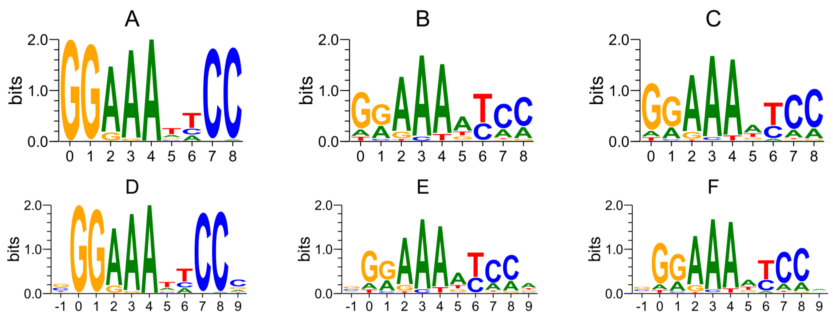
\includegraphics[width=6in]{plotcayatg.pdf}  %logos0_30bp.eps}
\caption{Logos generated for known Dorsal sites (the $D_{CB}$ data) tested for adjacency to 5'-CAYATG used as the cooperative class if in the [0,30]bp distance.  Logo A corresponds to the cooperative class, and displays the known 5'-AAATT core, with total information content 13.5 bits. 
 Logo D is the exact same logo as A but with a single base-pair of flanking sequence at the start and end of the site (hence, this logo starts at position -1).  Position 9 of this logo shows about two decibits of information relative to the background sequence in the nucleotide base `C' (2 out of 10 functional DC sites have a `C' at this position).  Logo B is the `uncooperative' class for the [0,30]bp window, which we calculated to have 9.1 bits information relative to the background (uniform distribution of bases), and logo E has the added flanking sites to the `uncooperative' class.  Logo C is the CB motif with 9.6 bits of information relative to the background, which looks similar to the 'uncooperative' class at position 6 due to there being many more sites that prefer A to a T at this position amongst all the Dorsal sites in the network.  Logo F is the CB motif with the flanking sequence appended.}
\label{logofig}
\end{figure}

\subsection{The conditional and unconditional PWMs are significantly different}
 
Here we test the optimal DC and DU detector's training data energy scores to see if the median energy of DC is significantly different than the median energy of DU.  The optimal detectors were based on the 5'-CAYAGT Twist motif and the [0,30]bp window.  The rank sum test rejected the null hypothesis that the median energies are equal with  $p=10^{-26}$.  The median energy of the DC PWM was 0.27, while the median energy of the DU PWM was 2.7.

It is possible that any random partitioning of a set of binding sites that are used to build detectors using our technique would produce p-values consistent with significance.  We used our original data set of Dorsal sites $\mathcal D_{\textbf{CB}}$ to construct a sampling distribution of p-values for the rank sum test 
 To calibrate the p-value we created a sampling distribution of the p-value from 1000 repetitions, where at each repetition the combined data $\mathcal D_{\textbf{CB}}$ were randomly partitioned into two data sets.  PWMs were constructed for each partition.  The energy of each sequence within a partition was calculated as $E(S)+w(S,P)$, where $P$ is the partition, $S$ is a sequence in the partition, and $E(S)$ is the CB energy.  We then determined the corresponding rank sum p-value between the random sets. We found that the p-value of the rank sum test between the DC and DU model fell  well beyond the right tail of the random sampling distribution (shown in \Fref{b}), indicating that the median energies of DC data set and the DU data set are significantly different from {\em any} random partitioning of the combined data set. More details are in the Supplement section \ref{ranks}. %section number [CA]
%Fig. 2
\begin{figure}
  \includegraphics[]{rsCAYATG30.eps}\\
  \caption {Histogram of p-values of a rank sum test of random partitions of the combined data set $\mathcal D_{\textbf{CB}}$.  The binning is in units  $-10\times \log_{10} $ of the p-value, rounded to the nearest integer. The p-value of the rank sum test between DC and DU energy data sets based on their energy PWMs was 260 in log base ten units (scaled by 10), which is indicated by the red bar of arbitrary height.   
   }\label{b}
\end{figure}


\section{Performance of optimal classifiers (detectors) }

All detectors were built from length 9 alignments (see Supplement section \ref{emalg}for details of the alignment procedure).
The OR gate is based on the DC detector built from the data set $\mathcal D_{DC}$, which contains Dorsal loci from  $\mathcal D_{\textbf{CB}}$ that were tagged with class labels from the optimal spacer window of [0,30]bp with the 5'-CAYATG motif, and similarly, the DU detector is built from the data set $\mathcal D_{DU}$, which contains the remaining Dorsal loci from  $\mathcal D_{\textbf{CB}}$ that did not have the Twist sites in the spacer window.  .  
The unbolded subscripts DC and DU on the data sets denote that these sets of Dorsal sites were based on our clustering scheme (not based on literature annotation). 

We now present three experiments that tests the performance of our OR gate detector and the conditional detectors using the CB PWM as a benchmark.

\subsection{The DC detector predicts sites proximal to 5'-CAYATG with better odds than the DU detector.}
We expect that DC should predict Dorsal binding site sequences that are adjacent to Twist more precisely than DU (since we showed earlier that the Dorsal site sequences contain information about adjacency to Twist).  In \Tref{tabless2} we collected all the hits (all the positives) of the detectors.  We test whether the DC conditional energy PWM is actually \textit{predicting} Dorsal sites within the CRMs that have the correct flanking sequence feature (presence or absence of Twist motif) with better odds than the DU detector.
The odds of DC for predicting binding site sequences that belong to the proximal class was $\frac{61}{39}=1.6$.  The odds of DU for predicting sequences of the proximal class is $\frac{280}{345}=0.81$, hence the odds ratio is 2.0.  The one-sided p-value for this table's log odds ratio test is $p=0.001$ for the chances of seeing a DC detector with better odds relative to DU at predicting correct flanking sequence features.  Increasing the energy cutoff $E_c$ increases the total counts of the table, and we obtain similarly significant tables up until about $E_c=5$.

\begin{table}[h!]
\centering
  \begin{tabular}{ r|c|c| }
\multicolumn{1}{r}{}
 &  \multicolumn{1}{c}{proximal}
 & \multicolumn{1}{c}{distal} \\
\cline{2-3}
$DC$ & 61 & 39 \\
\cline{2-3}
$DU$ &  280 & 345 \\
\cline{2-3}
\end{tabular}
\caption{Contingency table with the conditional detectors DC and DU represented along the rows and the class type distal and proximal represented along the columns. Each table element represents the number of sites predicted from each detector of each class type based on Twist sites (5'-CAYATG) and a CB energy cutoff $E(S)=E_c=2.1$.  %End of caption.
 }\label{tabless2}
\end{table}



\subsection{Both OR gate and CB detectors show high sensitivity with known sites as positives and CRM sequences as negatives }
In order to test the sensitivity and the specificity of the detectors we used the Receiver Operator Characteristics (ROC), which displays the tradeoff between optimizing predictive performance for `positives', while also optimizing for not detecting known `negatives'.  The True Positive Rate ($TPR$) is defined as $TPR=\frac{TP}{(TP+FN)}$, where the denominator is the total counts of True Positives ($TP$)and False Negatives ($FN$)).  The False Positive Rate ($FPR$) is defined as $FPR=\frac{FP}{(FP+TN)}$, where the denominator is the total counts of True Negatives ($TN$) and False Positives ($FP$).

We use the data set $\mathcal D_{\textbf{CB}}$ as our training set of `positives' ($TP+FN$) for both the CB detector and the OR gate.  The `negative' data set ($TN+FP$) is the set of all CRMs that contained a known binding site (i.e., the CRMs associated with $\mathcal D_{\textbf{CB}}$), where the bona fide sites (the functionally confirmed sites) are masked out.  Furthermore, within the CRMs we also mask out overlapping predicted binding sites based on the algorithm in the Supplement section \ref{overlap}, hence the negative data (the CRMs with known sites masked and overlapping hits masked) is at least nine fold smaller than the concatenated length of the CRMs due the binding sites being nine base pairs in length. 

For a given energy threshold, $E_c=E(S)$, set by the CB energy PWM for both the OR gate and the CB detector, each detector `scans' the CRM using a sliding window approach, where each `hit' of the detector is classified as a $TP$ if the hit overlaps a known binding site locus in $D_{\textbf{CB}}$, and as a $FP$ if the detector `misfired' in the background of the CRM.  Similarly, known sites (loci) from $D_{\textbf{CB}}$ that were not called hits by the detector are classified as $FN$, while $TN$ are the k-mers from the CRM background sequence that the detector did not call a hit.

The ROC of the OR gate (shown in \Fref{rocfig}A) tends to perform better than the CB detector at low energies up until the energy reaches about $E(S) < 8$ (the last point ($FPR,TPR$) displayed in the figure), after which the CB detector tends to do better.  The OR gate in the region of ROC space displayed shows better performance than the traditional CB detector (This is clearer quantitatively, where we found the OR gate had a higher area under the curve (AUC) integrated from the minimum energy to CB's energy cutoff of $E(S) < 8$ (which is the last point displayed in ROC space)).  The OR gate and CB detector both perform well for strong sites (low energy sites), which is indicated by their good $TPR$ (almost 80\% before a noticeable fraction of negatives start to be detected as positive.
%Fig. 3
\begin{figure}
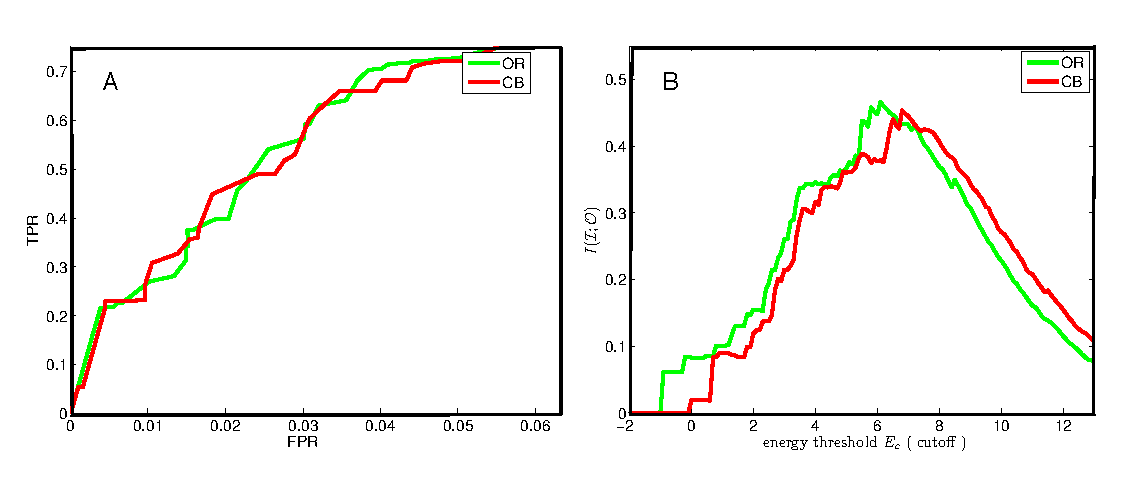
\includegraphics[width=6in]{infopair.pdf}
\caption{ROC and Information. (A) False positive rate ($FPR$) vs. True Positive Rate ($TPR$) when varying the energy cutoff $E_c$.  (B) shows the mutual information $I(\mathcal I;\mathcal O)$ Eq.~(\ref{inout}) between the input and output of the detectors as a function of the cutoff energy. }\label{rocfig}
\end{figure}


\subsection{The OR gate performs better than CB at predicting known sites at lower energies}
 Another metric of performance of the classifiers is the mutual information between the type of k-mer (Dorsal or not Dorsal) and the classification by the detector. For example, if the input is not a Dorsal binding site, the detector should stay silent, while it should fire if it is a Dorsal site (either adjacent to Twist or not). We can write this mutual information as
  \begin{equation}\label{miio}
  I(\mathcal I;\mathcal O)=H(\mathcal I)-H(\mathcal I| \mathcal O),
  \end{equation}
 where $\mathcal I$ is the binary random variable holding the true identity of the `Input' k-mer received by the detector, while the 'Output' variable $\mathcal O$ is the binary variable given by the detector's decision. The entropy $H(\mathcal I)$ is in principle given by the relative likelihood to find Dorsal binding sites within the ensemble of CRMs, which is of course heavily biased towards negatives (non-Dorsal sites). However, this Bayesian prior is not available to the transcription factor, in other words, for each decision to bind, the factor has its own Bayesian prior $p$, which we will set to $p=1/2$ (maximum entropy Bayesian prior) below. 


The conditional entropy $H(\mathcal I| \mathcal O)=-\sum_{i,o=0}^1p(i)p(i|o)\log p(i|o)$
quantifies the remaining uncertainty about the identity of the k-mer given the decision of the detector, and can be calculated using the false positive and true positive rates introduced earlier. In particular, the conditional probability $p(i|0)$ is obtained as
 \be
    p(1|1)=p(\mathcal I=1|\mathcal O=1) &=  TPR \\ 
   p(1|0)=p(\mathcal I=1|\mathcal O=0) &= 1-TPR\\
   	p(0|1)=p(\mathcal I=0|\mathcal O=1) &= FPR \\
   p(0|0)=p(\mathcal I=0|\mathcal O=0) &= 1-FPR \;,
  \ee 
while  $p(i)$ is the Bayesian prior (density of Dorsals/non-Dorsals in the CRM). Using an arbitrary prior $p$,   
we can rewrite the mutual information from \Eref{miio} as:
\begin{equation}
I(\mathcal I;\mathcal O)=H[p] - pH[TPR] -(1-p)H[FPR]\;,
\end{equation}\label{inout}
where $H[*]$ is the usual binary entropy function of a Bernoulli distribution characterized by *, so for example
 \begin{equation}
 H[TPR] = -\frac{FN}{TP+FN} \log{\frac{FN}{TP+FN}} -\frac{TP}{TP+FN} \log{\frac{TP}{TP+FN}}\;,
 \end{equation}
with a similar expression for $H[FPR]$.
We show the mutual information $I(\mathcal I;\mathcal O)$ in \Fref{rocfig}B using the maximum entropy Bayesian prior $p=1/2$.  Compared to the information the CB detector has about Dorsal sites, the OR gate's information is shifted to lower energies, implying that at fixed energy cutoff it knows Dorsal sites better than CB. 

\subsection* {DC conditional detector is able to predict that Twist is nearby} 
The conditional detectors are expected to make predictions not only about what is a Dorsal site relative to the background, but also whether Dorsal is in the vicinity of Twist.  By partitioning all the known sites into the two class types (e.g., `distal' and `proximal') as determined from the spacer window of [0,30]bp and Twist motif 5'-CAYATG, we can test how well each detector can resolve the class type of a Dorsal site (Dorsal with Twist or without).  

For a given energy threshold we scanned the combined data set $D_{\textbf{CB}}$ with the DC as well as the DU detector, and asked how much the detector knows about the class variable $\mathcal C$ (further details of this experiment are in Supplement section \ref{misup}).  We show this mutual information $I(\mathcal C;\mathcal P)$ in \Fref{MiSP} , where $\mathcal P$ is the binary random variable encoding the detector's decision about the context. 
\begin{figure}
  %Fig. 4
  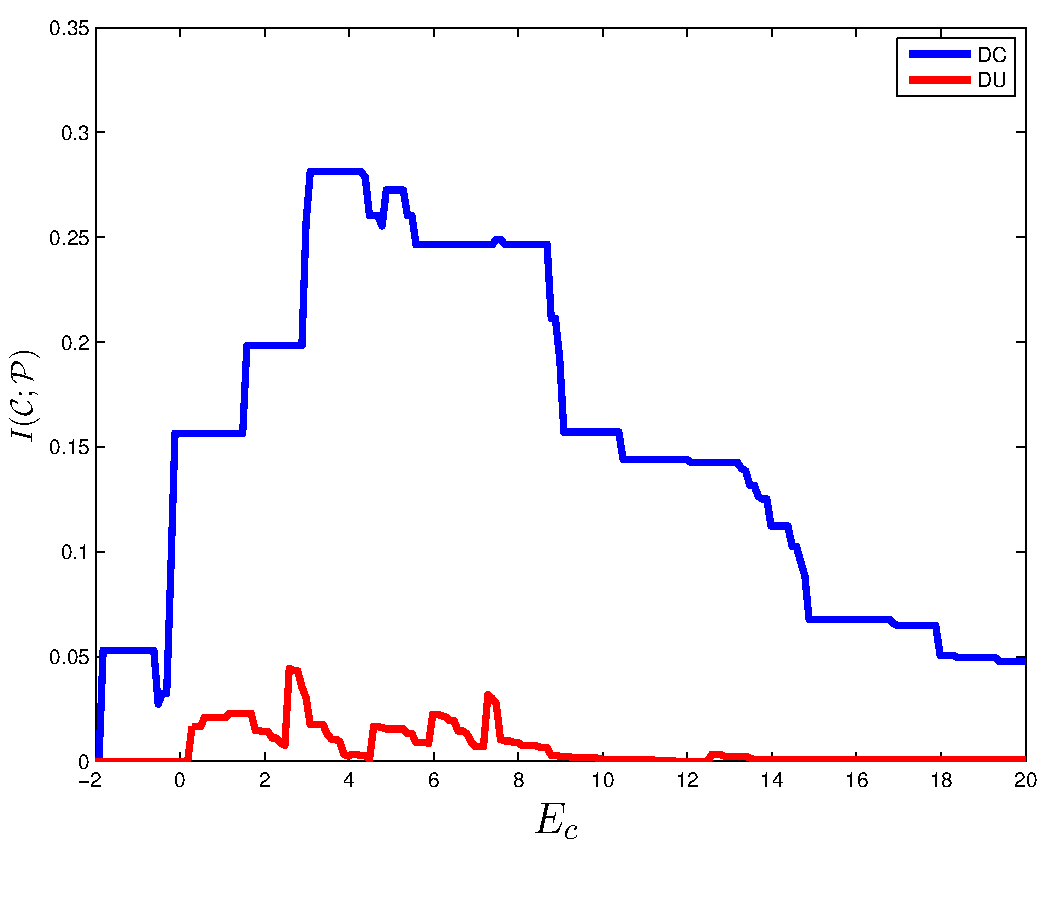
\includegraphics[]{miclasses-new.pdf}\\
  \caption{Mutual information $I(\mathcal C;\mathcal P)$ between the actual classes $\mathcal C$ and the predicted classes $\mathcal P$ for Detectors DC and DU as a function of the threshold energy $E_c$ that is defined by each detector's conditional energy \Eref{cepwm}.
    \label{MiSP}}
\end{figure}
We see that the DC detector has up to 0.3 bits of information about the proximity of Twist in any particular Dorsal site, while the DU detector has virtually no information about this variable. 

\section{Discussion}

\subsection{DC and DU Information logos and previous evidence}
The binding site sequence logos display the information content of our binding site data relative to a uniform distribution.  By inspection of the DC logo the consensus sequence (highest information scoring sequence) is partially consistent with Table S2 of Crocker et al.~\cite{pmid20981027}.  The 5'-AAATT core is reproduced as our DC consensus sequence, while the flanking sequence for the length 11 binding sites are not enriched with G at the start of the site and a C at the end of the site.  Similarly we can see that our DU also conforms roughly to A-tract Dorsal binding sites, which are Dorsal binding sites that have four or more contiguous Adenines.  Mrinal pointed out that A-tract binding sites have certain physical chemical properties not seen in 5'-AAATT core Dorsal sites~\cite{pmid21890896}, namely that A-tract Dorsal binding sites encode a mechanism (like an extra hydrogen bond between the protein and DNA) for Dorsal to switch roles from an activator of gene expression to a repressor of expression based on the binding site Dorsal was occupying.  Of course, as mentioned by Mrinal, these sites are still context dependent, namely the context of a site may override any preference a binding site sequence has for causing activator or repressor roles\cite{pmid1582412}.  Inspection of our DU detector's data set shows that it is more than 50\% enriched with Dorsal sites that are known to be from repression \textit{cis}-regulatory elements (\textit{zen}, \textit{tld}, \textit{dpp}), hence the DU logo with a 5'-AAAAT core is not surprising.

Our known binding sites, to a degree, come with the class labels already attached.  The $\mathcal D_{\textbf{DC}\textit{mel}}$ data is the known Dorsal binding site data set based on the definition of $\textit{D}_{\beta}$ or 'specialized' sites, or NEE-like Dorsal binding sites (neuroectoderm Dorsal sites that were linked to Twist sites, but were not linked to the canonical 5'-CACATGT Twist sites)~\cite{pmid20981027,pmid15026577}.
However, our DC detector is different than a detector built strictly from the $\mathcal D_{\textbf{DC}}$ data set (the set of all 12 orthologs for each {\em melanogaster} locus), since we included additional ortholog CRMs of the NEEs.  
 
Furthermore, within the NEEs one could imagine that the spacer has diverged in species that we analyzed that were not analyzed previously, and our choice of the spacer window is an interval not the same as previous choices. For example, Papatsenko et al.~\cite{pmid15795372,pmid19651877} showed that binning the spacers between Dorsal and Twist that there were various optimal bins (namely 14bp, 20bp, and 53bp). It is also possible that the spacer defining the distance of Dorsal and Twist in {\em D. melanogaster} has further diverged in its ortholog species, in particular those not previously analyzed and annotated. 

Szymanski \textit{et al.}\cite{pmid7774581} used DU-like Dorsal sites in his systematic study of the role spacing has between Dorsal and Twist site, suggesting that Dorsal Twist still cooperate if one uses a DU-like binding site, which is further corroborated by systematic studies from Fakhouri \textit{et al.}\cite{pmid20087339} that also used A-track Dorsal sites for the primary Dorsal sites.  These studies suggest evolution could have fixed either a DC or a DU type site at an NEE locus utilizing Dorsal Twist linked sites for synergy, which would deteriorate our claim that DC and DU are really different types of Dorsal sites.  However, it is highly unlikely that all these sites would have fixed with the same sequence unless they were functional or else if the CRMs containing them were duplications.   
\subsection{The OR gate and the CB detector}

The OR gate scores any input k-mer with both conditional detectors DC and DU, and then outputs simply the lowest energy score.  Similar detectors have been represented in the literature as a Hidden Markov Model or as a mixture model~\cite{pmid16236723,Hannenhalli01062005}.
Each component of the mixture is simply a conditional PWM, where the mixing frequencies are estimated as the fraction of training data that is associated with a particular component (or class) of the mixture.  The mixture is defined as:
  \begin{equation}\label{mixpwm}
P(S)=\sum_{c} \frac{\exp{-E(S|C=c})}{Z_c} P(C=c),
\end{equation}
where $E(S|C)$ is in units of $\lambda_1$ (which is further assumed to have been calibrated to thermal energy units), and $Z_c=\sum_{S\in \mathcal S} \exp{E(S|C=c)}$, where $\mathcal S$ is the set all possible k-mers, $|\mathcal S|=4^k$. 


The CB detector is the traditional position independent probability model (PWM) of binding sites, where the PWM is constructed by aligning all of the sites in the $\mathcal D_{\textbf{CB}}$  data simultaneously.
Recall from \Eref{pwm1}
\begin{equation}\label{cbpwm}
P(S)=\prod_i P(S_i).
\end{equation}
where, as a consequence of Bayes' Theorem $P(S_i)=\sum_c P(S_i|C=c)P(C=c)$.
However, for a sequence of bases, $\prod_i P(S_i)=\prod_i \sum_c P(S_i|C=c)P(C=c) \neq \sum_{c}\prod_i P(S_i|C=c)P(C=c)$, where the last expression is the mixture of \Eref{mixpwm}, and is equivalent to a marginalization of the sequence over the classes.  The mixture distribution of the sequence over classes can only be factorized as a product of position distributions {\em given} the class. 
We justify our approximation of the marginal sequence distribution over classes as a PWM (the CB PWM) in the Supplement section \ref{misup}. %Where exactly ? [CA]

 The mixture model was used by Hannenhali et al.~\cite{Hannenhalli01062005} in a similar form as the OR gate, where a given transcription factor's binding preference was described by two PWMs.  There the authors scanned a given CRM or promoter with both PWMs and selected the highest scoring sites as hits, where the threshold for a hit was determined by the mixing frequencies--the proportion of known sites that are used in constructing each PWM.  Upon scoring all the sites within their promoters, the scores were ranked for a given PWM, and then the fraction of sites equal to the mixing frequency were considered positives.  This method is different than the OR gate presented here in that we do not use the mixing frequencies in discriminating Dorsal binding sites from background DNA.  The OR gate discriminates sites from non-sites by checking if the minimum (i.e., best) score of the component detectors is below the energy threshold.  By always choosing the lowest energy score among the given components as the detector's overall energy score, the benefit of an increased True Positive Rate of the detector is partially cancelled by the cost of an increased False Positive Rate.  However, this cost is only in effect at high energies (non-specific sites), where it is unlikely that evolution or physical binding is having any functional effect on the organism.  Hence, the OR gate is a useful model for increased sensitivity in the low energy regime.


\subsection{The CB data set, merging and dividing clusters of binding sites}
   The mixture distribution of equation of \Eref{mixpwm} implies the data set $\mathcal D_{\textbf{CB}}$  over all loci can not be aligned simultaneously to form an estimate of $P(S)$, as that only makes sense if one is constructing the CB PWM, which assumes no mixture.  However, a priori, one may not know whether their set of binding site loci is a mixture of different types.  To determine if there is a mixture in the data one must decide on how one will align the mixture model, and whether that alignment should be related to the case that one combines all the data indiscriminately to form an alignment for the CB PWM.  Will all the training data over all classes be lumped together to estimate $P(S)$ for CB, and then the conditional probabilities estimated by partitioning their respective set of aligned sites?  This technique is commonly used in the case that one is given a set of \textit{aligned} data, and one wishes to find mixtures within the aligned data.  Alternatively, will the training data be partitioned into the classes, and then each class aligned individually, and then these class-specific alignments simply be 'merged' to form an estimate of $P(S)$ for CB?

This additional complexity is analogous to the decision made in clustering motifs as to whether one wants a top-down approach (start from the root and \textit{partition}), or a bottom-up approach (start from the leaves of the tree and \textit{merge} (i.e. combine)), see for example \cite{10.1371}\cite{Down01012005}\cite{Jain:1999:DCR:331499.331504}.  We presented results for a bottom-up approach that aligns the training data $\mathcal D_{DC}$ and $\mathcal D_{DU}$ separately to estimate each conditional PWM DC and DU, then CB was based on merging the count matrices of the DC and DU data sets.

The top-down approach aligns all the sites together, then partitions out the classes, and from those partitions builds (without further alignment) the conditional probability PWMs, $P(S|C)$.  The bottom-up method is guaranteed to achieve higher Mutual Information than the top-down approach.  This is because the DC alignment will not necessarily be 'in register' with the independent DU alignment, for example the DU alignment may tend to have the first character with more than 0.5 bits of information shifted relative to the DC alignment (i.e. the binding start site of these two set are shifted). This in turn causes their marginalization to have an increased entropy due to mixing alignments out of register, which in turn causes the mutual information to be boosted, since the conditionals are both now substantially different than the marginal due to registration of the start sites.  Based on results not presented, we found that the top-down approach still preserves the overall trend in Mutual Information verse spacer window, although the signal in the [0,30]bp window for distances of known Dorsal sites from the 5'-CAYAGT motif is reduced by about 40\%.

From a model comparison viewpoint, one may assume the strategy should be to align DC, DU and CB all separately, neither taking a top-down or bottom-up approach.  This strategy does not bias either the mixture model (OR gate) or the CB PWM model.  However, from results not presented, we found this has little effect on the logos for a length 9bp alignment.  Albeit, some alignments (in an ensemble of alignments derived from gibbs sampling) do choose a 'T' rich motif, as opposed to an 'A' rich motif.  For our logos, in the case that a 'T' rich motif was found, we presented the logo derived from the reverse complement of each \textit{aligned} sequence within the training data set so that all logos would be easily visually comparable by inspecting the logos.  For longer than 9bp length alignments of Dorsal binding sites, we found that the Conditional Dorsal motifs frequently were not in 'register', where registration of the start sites of motifs is based on a motif-motif alignment program like STAMP\cite{pmid17478497}, but can also be seen by inspection of the logos (sometimes).  For example, by inspection, the DC motif for a length 11bp alignment may have had the first position in the alignment with greater than 0.25 bits of information content at position one (in a zero based coordinate system), while DU would have its first position in the logo with more than 0.25 bits at position zero (the start of the logo).

From a physical standpoint, it may be that the conditional binding sites do tend to have a shift in their binding start site positions.  For example, Dorsal may bind to :  5'-AAGGAAATTCC in a DC favored environment, while in the DU favored environment it binds: 5'-GGAAATTCCAA.  If the flanking A's really are a signal, then one must conclude the best representation for CB would be: 5'-AAAGGAAATTCCAAA, which is a motif that is 3 nucleotides longer than either conditional.  The bottom up approach to clustering would miss this signal, since it would merge the two classes such that the CB PWM would contain a fraction of `A's at the first position based on the proportion of the DC data relative to the CB data, and another fraction of `G's at the first position due to the DU motif; thereby not only missing some of the signal, but also interfering with the captured portions of the signal.  This particular case shows that trying to compare motifs based on having the starting position of the motif being in register, will potentially truncate a signal for the CB model.  The logos in \Fref{logofig} are in register (the start of the binding sites are the same), which is based on our findings that length 9 alignments are the most reproducible in terms of registration.  Once we had aligned the length 9 binding sites, we then appended the flanking sequence to each already aligned locus, thereby having greater assurance that the CB PWM would not have this type of interference effects.

  However, if one starts with an alignment that has flanking sequence to begin with, (such as an alignment of length 15bp;) then one could try and discover if the \textit{aligned} sites do contain a mixture of motifs without having to worry about the problems associated with choosing a strand (such as the `A' rich strand), or whether the start sites are in register.  Such an approach was used in Figure 2 of Barasch et. al. \cite{barasch}.  However, we found that setting the Gibbs sampler alignment's length parameter highly influences the alignment.  For example, for a length 9bp alignment, the starting position of the alignment may contain maximum information (2 bits), however if one creates a length 15 alignment this signal (the information) is at least conserved, but may spread into the flanking sequence.  This spreading changes the DNA makeup of the logo of various positions.  This is partly due to there being so many more ways to spread out information among the positions of the alignment when one is using an objective function that runs over 15 positions as opposed to 9bp.  For example, a subsequence of 5'-AAA that is completely conserved in a length 3bp  alignment, when allowed to be length 5bp alignment may converge on 5'-AAAAA with the same information content as the 3bp alignment (or slightly larger information content than the length 3bp alignment, while having a smaller per position information content).  This is due to a mixture over loci of the form: 5'-NAAAN, 5'-AAANN, 5'-NNAAA.
  
  
\subsection{ Mixtures of asymmetric PWMs}
In the case that one's data set of binding sites is primarily asymmetric, yet completely conserved at each position; then one can construct a two component mixture of PWMs that are significantly different by simply choosing each component PWM to represent each concensus of the two asymmetric motifs.  For example if one's data set is simply a collection of loci from a database where the sequences from the database were all identical of the form 5'-GGAAACC, then one could take half the loci to be 5'-GGTTTCC, and the other half 5'-GGAAACC.  We found that when training the mixture model where one has no knowledge about what strand to use in the component PWMs (i.e. DC and DU) that DC and DU frequently would converge on motifs that appeared to be reverse complements of one another.  To resolve this problem one can symmatrize the PWM by using both strands in the construction of the PWM (see for example the paper by Bailey et.al.\cite{pmid7584439} and the discussion of MNT operator sites by Fields et.al.\cite{pmid9268651}).

A hypothetical DC concensus 5'-GGAATTTCC may seem to be a problem for symmetrization if the 'T' at position 4 (where the start site is position zero) would lose some of its signal by symmetrization.  However, in a sense, this loss would be compensated by a gain in its complement's 'A' signal if one considers the symmetrical PWM to contain a smaller alphabet of symbols.  \footnote{This compensation may seem to be violated due to the loss of information content when one symmatrizes a pure 'T' signal at position 4 of the DC motif.  However, the source of this apparent violation is due to comparing signals from two different sample spaces.  For example, the original alphabet of 'A,C,G,T' has at most 2 bits of information.  However, when one uses a symmetric PWM the alphabet size is no longer over 4 characters, but simply over 2 characters, hence the most the information can be is now 1 bit.  Hence if one compares normalized information contents (normalized by alphabet size), then the normalized information contents are preserved.  From another perspective the choice to symmatrize is an additional bit of information gained that compensates the bit of information lost by the original 2 bit 'T' signal.}   Even for highly non-palindromic sites such as the 'A-rich' core in the Dorsal DU sites, one could still symmatrize the motif and hence not have to deal with issues of strandedness of sites when forming mixtures of PWMs.  However, there are a number of reasons why mixtures of asymmetric PWMs is important, assuming one can deal with the potential artefacts such as a loss of the  signal due to choosing opposite strands (such as in the 5'-GGAAACC data set example above which would artificially boost the mutual information). 

Our decision to treat the component PWMs as 'asymmetric' PWMs was based on the assumption that the orientation of a site relative to cooccurring sites may be important, hence by using asymmetric PWMs we would allow ourselves the potential to decode any orientation information if it were encoded in the PWM(see Shutzaberger et.al. for more ideas on this topic of strand\cite{Shutzabergerpmid18030333}).  The potential to decode context information based on the strandedness, is equivalent to making predictions that a particular type of cooccurring binding site would be either 5' or in the 3' direction of the annotated binding site.  This decodable information would also be physically related to cooperative or antagonistic interactions that are contingent on the binding site sequence.  An example of this is the asymmetric extended Twist site 5'-CACATGT (extended from the E-box sequence CACATG, where a 'T' is concatenated to the 5' end of E-box), this site has evidence that the 'T' at the 5' end must cooccur with a Dorsal site \textit{downstream} of it (i.e. where downstream means in the 5' to 3' direction)\cite{pmid16750631}.  For example, one would always find evolution selected 5'-CACATGTNNNNGGAATTTCC and never find 5'-GGAATTTCCNNNNCACATGT.  Furthermore, one could imagine that the Dorsal site that cooccurs on the same strand in this case is 5'-GGAATTTCC, as opposed to 5'-GGAAATTCC, where position 4 is strand dependent.  In this case, had one symmatrized the DC PWM they would have lost the information at position 4.  Hence the higher information content of the asymmetric PWM is not an artefact of the asymmetric PWM \footnote{This may be an artefact in that asymmetric PWM's always have greater (or at least equal) information content then symmetric PWMs}, it's rather telling us that this is physically due to the preference of the 'A' at position 4 of the DC motif cooccurrring on the same strand as the annotated Twist site (i.e. 5'-CACATGT).  Similarly the DU concensus' core '5-AAAAT' may be cooccurring on the same strand as other coregulating trans factors, and hence cooccurring with other motifs on the same strand.       
	
\subsection{Comparing models with unequal parameters}
 For optimization and model comparison, models that have more parameters may be guaranteed to have a higher likelihood value for a given data set, just as a Taylor expansion approximations of a function improves when one includes higher order terms.  Assuming one has sufficient data to stay clear of fitting parameters to noise, and that the more complicated models are a more accurate description, a more complicated model may be useful.  However, it is not true that the OR gate, must perform better than CB due to the increased number of free parameters.  
 
 In detection, ensemble classifiers (such as the OR gate) can be used to increase the detection performance\cite{bishop}.  However, it is not true that \textit{ensemble detectors} will always perform better than a single detector.  The OR gate is a form of the more general ensemble detector that is a machine that produces a decision based on component detector decisions, where the component detector's decisions are pooled and processed in order to come to one overall decision of the ensemble detector.  Examples of processing the individual detector's decisions are 'majority vote', where the most frequent decision of the collection among the component detectors is used as a the final machine's decision, similarly the OR gate is an example of an ensemble detector.  Ensemble classifiers have a necessary condition to perform better than a single classifier: the component classifiers (e.g. DC and DU) should be independent of each other\cite{bishop}.

DC and DU are independent if we use a conditional independence model for the joint distribution of an extended sequence S, where we now think of the extended sequence S as a dyad (which can be decomposed into three variables that denote two bindings sites separated by a variable spacer, like in the framework of BioProspector).   In this probability model over the joint we partition an extended sequence S (like a CRM) into two parts, S' and C, where S' is the k-mer sequence to be tested as a Dorsal site or background, and C is the class determined by the \textit{spacer window}, which either contains Twist or it doesn't.

Given that we observe the class C, then we can factorize the joint distribution of the sequence S' being tested as a Dorsal site (i.e. S' is no longer a position dependent distribution). Without the above assumption DC and DU are dependent, hence the OR gate, which does not observe the class C, does not have independent component detectors.  A consequence of this dependency is that the component detector's errors are correlated (i.e. misclassification errors are correlated).  For example, each component classifier's probability of a base 'G' at a given position in a binding site should be just as likely to be above the true value of the probability of G, P(G), as it is below the true value; while for correlated detectors this does not occur.

Hence, it is not always true that increased complexity of a model will increase its performance on training data.  Mixture models of binding sites are more complex than a standard PWM, and are best at capturing broad dependencies among the component classes.  To a large extent, the difference of DC and DU is a localized dependency at particular position (which can be seen as the difference of their cores '5'-AAATT' and '5'-AAAAT'), and a differences in the 'strength' of the sites (or the energy level spacing).  The OR gate seems to perform better than CB for the low energy regime, where the localalized difference between the cores of DC and DU is significant in distinguishing the energies of the concensus sequence of each conditional PWM.  However, for the entire energy spectrum, where AUC can be used as a measure of performance, it seems the OR gate behaves about the same as CB, suggesting that DC and DU are not independent models.  This is not surprising, as nonlinear models (like a mixture) are sensitive to certain regimes over their input, and similarly insensitive to certain values of their input (for example see Section \ref{overdeter}.    
  
  

 \subsection{Information that detectors have about Dorsal binding sites}
In a physical NVE ensemble (fixed particle number $N$, fixed volume $V$, fixed energy $E$) the information content of the distribution of momentum and positions (the distribution function) is conserved.  This means the number of bits necessary to store the position and momentum information is conserved in time relative to the maximum storage capacity defined by a lattice over phase space (the space of coordinates).  For example, if the distribution function is a uniform distribution over phase space, it has zero information content.  

Similarly, evolutionary systems under adaptive maintenance (purifying selection) conserve information stored in their genes~\cite{pmid22320231}.  The inheritance of information implies that parents pass a fixed number of bits to their progeny.  And just as in the NVE ensemble where coordinates and momentum are not conserved, similarly in evolution sequences are variable, but the sequence's  information content is conserved.  However, when the fixed energy constraint of the NVE system is relaxed and the system exchanges energy with a much larger environment, the system's original information content may deteriorate until the system equilibrates with its surroundings. Biological systems harness energy from their environment to maintain their information content in the never-ending fight against the second law~\cite{Adami2002,Carothersetal2004}.

 The mutual information between sequences and the OR gate's predictions in \Fref{rocfig}  suggests that the conditional distributions of functional Dorsal binding sites have encoded synergistic and antagonistic information about flanking sequence features (presence of Twist) that causes the likelihood to correctly predict the presence of Dorsal to shift downwards in energy (as observed by the shift of the mutual information of the OR gate relative to CB in \Fref{rocfig}).  This shift may have been a necessary adaptation in the way Dorsal regulates its targets.  For example it is possible that at the phylum level, possibly before the neuroectoderm evolved, Dorsal only needed to regulate the mesoderm and ectoderm. When the neuroectoderm evolved, Dorsal evolved the ability to recognize two subtypes of binding site ensembles, a function that would help to resolve the neuroectoderm Dorsal targets from the more ancient germ layers (mesoderm and ectoderm).  In this sense, Dorsal's adaptation to its local environment is seen as the shifted mutual information relative to the CB detector (which just treats all binding loci identically).  Dorsal could then use this information to its advantage, in Dorsal real time so to speak, to make better decisions about binding.    
  
 The shift in the mutual information plot in  \Fref{rocfig}B is not as visible in the ROC curves in \Fref{rocfig}A, in which we used the same TPR and FPR for the detectors.  This is because, in general, energy level spacing is not accounted for in an ROC curve, implying that detectors with similarly ranked sequences may actually have different spacings between their energy levels, and the minimum energies of the scales may be shifted relative to one another.  For example, DC's ground state is below CB's ground state, which is why the OR gate contains some information at negative energy (as DC's ground state is at about -0.8 in energy units as seen from the horizontal axis of \Fref{rocfig}).
     
 The degree to which the OR gate's ROC does appear shifted relative to CB's ROC in \Fref{rocfig}A is partly due to the fact that the ranking of sequences of the DC detector and DU detector is very similar; it is the energy level spacing that is dramatically different between the conditional detectors.  For example, using a substitution model that penalizes all mismatches from the consensus sequence with the same energy score (see the Appendix of Ref.~\cite{pmid3612791} for details) leads to the elegant formula that a consensus base occurs with probability $1-\frac{m}{3k}$, and that an error or substitution occurs with probability $\frac{m}{3k}$, where \textit{k} is the length of the sequence and \textit{m} is the number of mismatches from the consensus (the 3 in the denominator is due to the three ways a mismatch from a consensus DNA nucleotide can occur).  Weak sites will be seen to have large \textit{m}, which to a degree can be seen as the DU training data. Similarly, strong sites will have small \textit{m}, which can be seen as the DC data.  Hence in this substitution model, the difference between DC and DU is not in the ordering of their ranked sequences, rather the difference lies in their energy level spacings (which can be seen by changing $m$ which affects the energy spacing formula \Eref{epwm2}).  
 
 This picture of DC functional sequences being a strong version of DU's sequences is consistent with our findings that their median energies differed by almost two units, and with Papatsenko \textit{et al.}'s findings~\cite{pmid15795372} that Dorsal binding sites necessary in limiting concentrations of Dorsal protein (such as in the neuroectoderm) tend to have higher information scores (lower energy scores), than other Dorsal sites such as sites active in the mesoderm~\cite{pmid15795372}.  It is also consistent with the mathematical definition of ``specialized" sites from Erives \textit{et al.}\cite{pmid15026577} and the $D_{\beta}$ sites of Crocker \textit{et al.}~\cite{pmid20981027} who defined these sites based on how they were detected (similar to MEME's One Occurrence Per Sequence setting (OOPS)\cite{pmid7584439}, the specialized sites were one site per NEE CRM sequence, where each discovered site shared the highest sequence similarity between the selected sites between the CRMs), which in a sense, is the Dorsal site that had the slowest mutation rate (i.e., under the strongest purifying selection).       
\subsection{Conditional detectors}


In \Fref{MiSP} we see that the DC detector can resolve whether a Twist site is in the spacer window or not if the detector fires when $E(S|C) < 3$ (see \Eref{cepwm}). The resolution is not perfect in this regime: the DC detector still has an error rate, which we define as $1-2^{-H(\mathcal C| \mathcal P)}$, where the conditional entropy is defined as:
\begin{equation}\label{conduncer}
H(\mathcal C| \mathcal P)=H(C)-I(\mathcal C; \mathcal P).
\end{equation}
The conditional entropy, $H(\mathcal C| \mathcal P)$, is simply the uncertainty of $\mathcal C$ given $\mathcal P$.  But what does this mean for a DC detector?  We interpreted this conditional uncertainty as a measure of the detector's uncertainty about the underlying Dorsal binding site sequence given how well it predicted its context.  For example, if we assume $H(\mathcal C)=1$ bit while DC's information is $I(\mathcal C; \mathcal P)=0.3$, then plugging into \Eref{conduncer} we have
\begin{equation}
H(\mathcal C| \mathcal P)=1-0.3 = 0.7\ {\rm bits},
\end{equation}
and hence Dorsal has decreased its uncertainty about its context.  

If the mutual information $I(\mathcal C; \mathcal P)$ was maximal (1 bit), then Dorsal could predict with perfect accuracy whether Twist was proximal or distal.  At the opposite extreme where the Dorsal detector does no better than random guessing, we see that it would take about two guesses on average to predict if Twist will be near a binding site sequence.  From an evolutionary point of view, the information $I(\mathcal C; \mathcal P)$ encoded in Dorsal binding sites can be seen as a message passed from an ancestral population of flies to its descendants.  Here, the message instructs Dorsal to interact with Twist, and is encoded in the DNA of Dorsal binding sites. 


\subsection{Forms Of Conditional Detector's score}
We have defined the conditional energy as the CB energy plus a shift depending on the cis-context of the binding site locus.  A similar bioinformatic measure is to solely use the conditional probability distribution over sequences to construct a bioinformatic scoring function as: $\log{\frac{P(S_{o_C}|C)}{P(S|C)}}$, where $S_{o_C}$ is the consensus sequence under condition C.  This form of the discriminant function can be transformed to our form $E(S|C)=\log{\frac{P(S_o)}{P(S)}} - \log{\frac{P(S,C)}{P(S)P(C)}}$ by a simple additive term to the bioinformatic score $\log{ \frac{P(S_{o_C}|C)}{P(S_o)}}$, where $S_o$ is the concensus sequence of the CB distribution.  The advantage of our technique is that mixture of data sets of different sub-types of binding sites that are heavily weighted by the consensus sites of the mixture component distributions can be shifted relative to the consensus site of the lumped data set, such as $\mathcal D_{\textbf{CB}}$.  Hence, we are able to resolve quantitatively the amount of energetic shift, while a purely conditional based scoring functions will set each detector's consensus score to zero.  Information scores $I(S)=\log{\frac{P(S)}{P_o(S)}}$, or log likelihood ratios, are also commonly used for bioinformatic detection, which can be transformed to our score by adding an additional conversion term that cancels the logarithm of the background distribution.  Information scores have the advantage over purely conditional energy scores in that they allow all bioinformatic scores to be based on a common scale (the background), which is equivalent to an energy score with a common reference point in the case that one uses a uniform distribution as the background.  This is because in sequence space\footnote{In this context each position of a sequence can be thought of as a 4 dimensional real vector space.  Then the length k sequence is 4k dimensional real vector space, where each point simply determines the scaling along each dimension (such as the counts that a particular nucleotide base is observed in an alignment at a given position, or the energy score at for that base at a given position).} one can imagine a point that represents a uniform linear combination of all sequences, then the information scores can be seen as hamming distances away from that point; just as energy scores are basically hamming distances measured from a reference point in sequence space.  Our aim was more than just discriminating Dorsal sites from random k-mers, we wanted to resolve differences within Dorsal binding sites.  Our score has the advantage of allowing one to resolve the most important region of that scale (shifts away from the CB ground state), which can not be done with the pure information score that uses a uniform background.
\section{Conclusion}

Position Weight Matrices represent a linear coarse-grained physical lattice model of DNA-transcription factor binding.  At the DNA sequence level and at the level of Darwinian selection PWMs represent one of simplest possible linear models.  In the case that each position within a binding site is independently interacting with the protein binding domain, it makes sense to use a simple model for binding since the affinity (the phenotype) is linear, and hence natural selection may behave as if a linear model.  However, binding site sequences may be dependent, and hence linear models will miss important information.  By conditioning PWMs based on the variables that are causing the dependency structure within binding sites it is possible to resolve the binding sites into independent classes that can then each be modeled as conditionally independent PWMs.

The necessity of introducing nonlinear sequence models into binding site sequence models is known to help improve binding site sequence detection, and to give a more realistic perspective to binding site models.  A number of groups have introduced similar models for discovery of co-occuring motifs~\cite{liu2001bioprospector,pmid21486752,pmid16873468,pmid14762058},\cite{barasch,pmid18426806,pmid19286833,GuhaThakurta01072001,gadempmid19193149,Moses04phylogeneticmotif}.  In addition, others have looked at the influence of symmetries in the flanking sequence of binding sites~\cite{pmid21723826,pmid25313048}.  Here we placed our analysis in the context of Berg and von Hippel's population genetics model that is related to thermodynamics, and hence the interaction term could be placed inside of thermodynamics occupancy models of transcription factors.

Our conditional PWMs account for epistatic interactions between Dorsal binding sites and their \textit{cis}-context.  We showed that Dorsal binding sites contain on average around 0.5 bits of information about the presence of Twist in the flanking sequence of each Dorsal site (see Table 1), thereby contributing to disentangling the dependency structure of Dorsal binding sites active in fly development.  In the future, our model can be incorporated in the annotation of binding sites of regulatory regions, and could be used for modeling cooperativity and antagonistic interactions directly from the sequence level. Such models could be used by occupancy models of transcription factors that predict gene expression, such as those in Refs.~\cite{pmid20862354,pmid20087339}. 

\section{Methods Supplement}


\subsection{ Alignment of cis-regulatory modules and collection of $\mathcal D_{\textbf{CB}}$} \label{muscle}
	We used the sequence editor SEAVIEW's default MUSCLE multiple sequence alignment settings \cite{pmid9021275} to align a given gene's 12 orhthologous CRMs\cite{BSA}.  Given the alignment we then manually extracted the blocks that contained the known $\textit{D. mel}$ binding sites, which allowed for flanking sequence to be extracted (these blocks on average spanned about 15bp with no gaps across the 12 species).  The data set of all 12 extracted orthologs (sometimes less than 12 if a binding site was not in the block) for all the $\textit{D. mel}$ Dorsal binding site loci is labelled as $\mathcal D_{\textbf{CB}}$.  The $\mathcal D_{\textbf{CB}}$ data set is available at: https://github.com/jacobclifford/MIBBS, and the raw CRM data (the fasta of each of the 12 orthologous CRMs) is available at:  https://github.com/jacobclifford/CRMalignment.
	
\subsection{CRM alignment using MUSCLE}
MUSCLE (multiple sequence comparison by log-expectation) is an alignment tool for protein sequences, which we co-opted for alignment of cis-regulatory modules.  MUSCLE uses a similar algorithm to CLUSTALW, both of which use the 'sum of pairs' (SP) objective function to determine the best multiple sequence alignment (MSA).  I will briefly outline the SP score, and then discuss how MUSCLE is different than CLUSTALW. 

  Fundamentally sequence alignment for strings of amino acid symbols or strings of DNA symbols rewards symbol matches and penalizes mismatches.  A scoring system is designed to determine the rewards and penalties based on the goals and purpose of the alignment, where the Altshult (the BLAST cofounder) and Karlin system is commonly adopted due to it having an analytic solution for calculation of the \textit{p}-value for hypothesis testing (where the null hypothesis is that the sequences are evolutionarily independent (random)).  

Regardless of whether one has a sequence of amino acids or DNA the match and mismatch score is based on a 'similarity matrices' such as a Dayhoff matrix (a 20x20 matrix for amino acids) or a Henikoff matrix, BLOSUM, which is essentially a look-up table that determines the score for aligning any two symbols (the table treats all positions of the sequences the same, unlike PWMs).  For example, Dayhoff estimated her similarity matrix partially based on recently diverged proteins from a number of known protein families (gene families) that were available at the time of construction (around 1970) with sequences that had a known alignment, then counting the frequency of alignment between any two symbols and hence substitutions between symbols, the joint probability, $p(x,y)$, of seeing symbol $x$ at some arbitrary time and symbol $y$ at some different time could be determined.  Hence the score is simply $s(x,y)=\log{\frac{p(x,y)}{p(x)p(y)}}$, where $p(x)$ is the probability of symbol $x$ in any protein sequence (similarly for $p(y)$).      	
	
	For pairwise alignment (two sequences being aligned), given a scoring system, there are two exhaustive methods of alignment (i.e. that look at all possible ways to align the two sequences).  These two methods are distinguished based on their 'boundary conditions', and are called global and local.  Global alignment means all they symbols of the sequences must be aligned and the score across all the aligned symbols must be accounted for in the pairwise alignment score, where the best pairwise alignment (the optimum) is a function over all possible alignments) .  While local alignment does not require all the symbols of the sequences be aligned, and the best subsequence pairwise alignment is considered to be the alignment, where now the pairwise alignment score simply accounts for the length of the subsequences, while again the best scoring aligned sequences is taken as the optimum.  Both methods, global and local, assume that no transpositions (or crossing over) occur (e.g. one must align consecutive characters of a sequence to consecutive characters of the other sequence or to a so-called indel character (gap or insertion) ). In short, global alignment means all characters between the two sequences must be aligned (with the possibility of gaps and insertions), while local alignment means only a subset of the character between the two sequences must be aligned.
	
	The pairwise alignment score of two sequences x and y that are clones of one another is $d(x,y)=\sum_i^L s(x_i, y_i)$ where i is the internal position of each sequence, and L is the length of the sequence.  If we now allow gaps between these sequences there are a total of $2n \choose n$ possible scores (many of which are degenerate).  The gap penalty is usually of the form of a constant (independent of nucleotide or amino acid symbol aigned to the gap).  For example, for a simple scoring system where $s$ is 'one' for a match, and 'zero' for a mismatch (the identity matrix), and we only have a constant gap penalty, we see that there is simply $L+1$ possible pairwise alignment scores from the $2n \choose n$ possible alignments.  In general, the computation of the $d(x,y)$ is accomplished through dynamic programming, where one has a progressively computes the global optimal $d(x,y)$ alignment by using the recursion relation $S(x_i,y_i)=max( S(x_{i-1},y_{i-1}) +s(x_i,y_i), S(x_{i-1},y_{i}) - g, S(x_{i},y_{j-1})  -g)$, where $S(x_i,y_i)$ is the partial sum of scores up to position $i$ for sequences $x$ and $y$, and $g$ is the gap penalty.    
	
	Once one has chosen what type (global or local) of pairwise alignment (i.e. $d(x,y)$ score) then to estimate a MSA for $n$ sequences using a SP objective function one must create a $n$ x $n$ distance matrix (same idea as in \ref{knownloc}), where the elements of the matrix are the pairwise alignment scores between any two sequences ($d(x,y)$).  Once one has a distance matrix any number of clustering algorithms can be used to begin to group sequences based on similarity, in particular a minimum spanning tree must be built.  Upon construction of the minimum spanning tree a pairwise alignment is arbitrarily chosen and sets the foundation of the MSA (a pair of leaves in the tree), then additional sequences are systematically 'added' to this foundation, where upon each addition the MSA grows until all $n$ sequences have been 'added' to the MSA.  The addition of sequences to the initial foundation is not arbitrary, the entire point of computing the minimum spanning tree was to guide precisely when each sequence should be added to the growing MSA (see figure 1 of Edgar\cite{pmid15318951}).  Hence MSA grows (is built) by following the branching of the tree, where at each branch point an alignment occurs.  This is called progressive alignment, and is the basic idea behind CLUSTALW.  For example, given the minimum spanning tree (suggestively called a guide tree) the first alignment is simply the pairwise alignment already calculated; the rest of the alignments are 'profile-sequence'-alignments - where a profile is an existing alignment (it is like a PWM with the possibility of gaps as a symbol), or a 'profile-profile'-alignment (where the columns of a profile are now regarded as a symbol, and standard global or local alignment is performed on these symbols, similar to STAMP for PWM-PWM alignments, where the 'match' function between two columns is called the profile function (which is called the log expectation score in MUSCLE).  
	
	A novelty of MUSCLE, as suggested by the LE in MUSCLE, is the log expectation score used for profile-profile alignment (see Eq. 1 from Edgar\cite{pmid15034147}).  Furthermore, MUSCLE also uses a $k$-mer counting scheme to determine the matrix elements of the distance matrix (as opposed to the global or local pairwise alignment score), where it is thought that $k$-mer co-occurrences correlate well with sequence similarity (see Eq. 1 of Edgar\cite{pmid15318951}).  The $k$-mer counting scheme is similar in spirit to the BLAST algorithm (local alignment between a short and long sequence), which is popular for its speed and high throughput (time and space computational complexity).  It appears MUSCLE looks at all possible 6-mers when constructing the similarity measure (and doesn't count overlaps). 
	
	The MUSCLE algorithm coarsly is shown in Figure 1 of Edgar\cite{}.  The initial step is identical to CLUSTALW with the exception that MUSCLE uses $k$-mer counting to define it's distance matrix elements.  And MUSCLE uses UPGMA clustering to build the guide tree, while CLUSTAL (CLUSTer ALignment) uses neighbor-joining, for reasons discussed by Edgar\cite{}.  The initial guide tree is then used to progressively align the data based on the branch ordering of the tree, where MUSCLE uses the LE score while CLUSTAL uses a LA score that is slightly different score (the difference between LE and LA is the same difference as our using a CB PWM to define P(S) and the true mixture to define P(S), where a true mixture can not be 'additive' when the logarithm is used for scoring).
	
	Upon construction of the MSA based on the guide tree, MUSCLE repeats the entire procedure using the Kimura distance to build a distance matrix (the Kimura distance requires an alignment, which is possible, since the initial iteration in MUSCLE constructs an alignment).  Clustering is again performed on the distance matrix (with matrix elements based on the Kimura distance between any two sequences), and again the guide tree (representation of clustering) is used to progressively build the new MSA.  
	
	A third type of 'iteration' occurs in the MUSCLE algorithm (after the newly generated MSA from Kimura distance), where the guide tree is randomly partitioned into two subtrees, where a profile (MSA) is built using each subtree as a guide  (the profile is progressively built, and hence an MSA).  Then profile-profile alignment is performed (similar to STAMP PWM-PWM alignment).  The number of random partitions of the guide tree, and hence profile-profile alignments is a parameter the user can adjust, or will automatically halt once the partitions fail to improve the alignment.  
%	, along with a Fasta file of the $\mathcal D_{\textbf{DU}\textit{mel}}$ and $\mathcal D_{\textbf{DC}\textit{mel}}$ sites that contains pubmed ID of at least one paper that verified the binding site, the REDFLY record number of each site (if it was footprinted), and the primary author of the pubmed article.
\subsection{MUSCLE is both fast and accurate }

There is almost always a tradeoff between speed and accuracy in computation.  According to the online MUSCLE documentation at http://www.drive5.com/muscle/manual/accurate.html: "The default settings in MUSCLE were chosen for best accuracy rather than making any compromises for speed, so if you want the best accuracy you should probably stick with the defaults unless you have a new and better parameter tuning method."  This suggests that our use of default parameter settings for CRM MSA would result in best possible alignments from the MUSCLE tool.  However, MUSCLE was designed for protein alignments, and even for protein alignments, the use of limited availability of high quality benchmark datasets means the MUSCLE parameters were tuned to fit a small subset of protein familys and their peculiarities, hence the generality of the MUSCLE parameter settings beyond these few protein familys in the benchmark datasets is questionable.

The speed and accuracy of MUSCLE for a given data set is determined by the number of 'iterations'.  Faster alignments are achieved by simply reducing the number of iterations, and more accurate alignments are achieved by simply increasing the number of iterations.  The 'iterations' that can be adjusted (as a parameter) are the 'refinement' iterations, which randomly deletes a branch of the guide tree, and then does a profile-profile alignment on the two subtrees (i.e. the two data sets of sequences resulting from the partition (branch deletion)).    
\subsection{MUSCLE parameter sensitivity }



A possible parameter that our CRM alignments, and hence our CB data set $\mathcal D_{textbf{CB}}$, are sensitive to are the choice of substitution matrix (especially seeing an amino acid 'substitution' doesn't even make any sense for CRMs, albeit using a substitution matrix for aligning regulatory sequences is unlikely to do harm, seeing that in all cases a substitution matrix rewards exact matches, the problem is it will also reward certain cases of mismatches or at least fail to penalize the mismatch.).  However, by default, if a DNA sequence is given to MUSCLE the substitution matrix is not used (presumably, because the reading frame is not known, albeit some MSA tools (unlike MUSCLE) will generate all possible reading frames automatically (there's only three of them)).  Furthermore, although MUSCLE leaves the option of using BLOSUM or PAM matrices for constructing distance matrices, as I understand, the default of MUSCLE uses $k$-mer counting as the distance measure, which I see no $a priori$ reason why that can not be used for CRMs.  An exhaustive list of parameters (options) for MUSCLE are described in the Command Line Reference section at:  http://www.drive5.com/muscle/manual/valueopts.html.   The Seaview editor allows these options (parameters) to be varied by setting them in the 'Alignment Options' tab available from the 'Align' pulldown menu available through Seaview's toolbar at the top of Seaview's GUI window.

MUSCLE uses an 'affine' gap score (penalty) that penalizes for opening, extending, and closing a gap.  This is the same scoring technique as CLUSTAW, and like in CLUSTALW, by increasing the gap score by a factor of ten will usually have visible effects by causing less 'blocks' to appear in the finished alignment, where the blocks that do appear are commensurately longer.  The default gap open score was 10, and this value I found, in some cases could be possibly be increased by an order of magnitude, as some known binding sites that have had indels will likely have a gap inserted in the final alignment (which creates more work for me, as I prefer to have the binding site block to have no gaps, which allows for faster 'sites' creation where we extract the block of putative sites and the known $mel$ site.  This is done by exact search in the seaview editor for a known $mel$ site in the CRMs.  Once found the site and everything it had aligned with/to are extracted and placed in their own fasta file; which is done in seaview by using the 'site' pulldown menu, and selecting 'create set' that allows for highlighting blocks (subsegments of an MSA) of aligned sequence, which can then be automatically saved as new fasta files. ).

The 12 CRMs that are associated with each target gene along with shadow enhancers (a distinct set of 12 CRMs associated with some target genes, such as \textit{vndV} (\textit{vnd Ventral}) and \textit{sogS} and \textit{brkS} (\textit{brk Shadow}) - where many of the shadows we did not use, such as \textit{vndV} and \textit{brkS}) are available at:  https://github.com/jacobclifford/CRMalignment.   


\subsection{GEMSTAT modifications for locus annotation of CRMs}\label{knownloc}
	 Given the known sites, $\mathcal D_{\textbf{CB}}$, with their flanking sequence from the block alignments we then created an exact search algorithm that allowed us to estimate the coordinate of the known site within the regulatory region for data structures used by GEMSTAT, a platform developed in the Sinha lab~\cite{pmid20862354}.  This program has a various inputs, which are irrelevant for our current purposes, the relevant input is a set of PWMs that represent transcription factors, and the set of CRMs regulated by these factor's motifs (PWMs).  We extended the GEMSTAT input to allow for a raw Fasta set of variable length binding sites (namely our Fasta file for the data set $\mathcal D_{\textbf{CB}}$).  Each of these sites and its reverse complement was transformed to a probability PWM 'singleton' representation ( the probability is equal to one for the observed nucleotide and zero for the other nucleotides).  The longest binding site of length n in the Fasta file determined the length of all the singletons.  Binding sites in the Fasta file that were of length k, where $k < n$, then had $d=n-k$ columns of zeros 'padding' the last d columns of their singleton PWM.
	 
	 We then constructed a distance matrix from the singletons, where each singleton is represented by a row and column in the matrix.   The matrix elements of the distance matrix were defined as a normalized euclidean dot product between the singletons (where corresponding components of each singleton multiple each other).  The normalized dot product between the singleton $S^x$ in row x and singleton $S^y$ in column y is defined as sum over all the element-wise multiplications:
\begin{equation}
	S^x \bullet S^y   = \frac{\sum_{ij}^{nn} S_{ij}^xS_{ij}^y}{\sum_{ij}^{nn}S_{ij}^xS_{ij}^x}.
	 \end{equation}	 
	 The row singletons are used for normalization, and hence for a given row x, by iterating over all columns we can filter out any identical singletons.
	 
For example, if we have 400 positive strand binding sites in our Fasta file, we will have a 800x800 distance matrix (400 of the rows corresponding to positive stranded sites, and another 400 rows for the negative strands); where the matrix elements are normalized Euclidean dot products between any two singletons.  By screening the distance matrix for elements that were equal to 'one' (which stands for a duplicate sequence or possible symmetric sites) we are able to determine which singletons are unique.  Asymmetric sites contain an instance for each strand (which means they are not unique), which is accounted for in our 'overlapping' sites processing step.  
	 
Collecting all the unique singletons, we then annotate (scan) the CRMs with each unique singleton using exact match (\textit{e.g.}, zero 'energy' singleton PWM threshold).  This step allows us to map each binding site in our Fasta file to a unique locus within the CRMs, thereby attaining the coordinates of all our known binding sites within the CRM coordinate system, which is an essential step in the spacer calculation of \Eref{cluster}.  
	 
Each unique singleton has a personal factor identification (a name), which we mutate to the name 'Dorsal' for every singleton.  Associating the name 'Dorsal' to the annotated sites within the CRMs is a necessary step in order to compute the spacer between each of the annotated 'Dorsal' sites and any predicted motifs sites within each CRM.  The coordinate defines the start or end of a binding site depending on what strand of the CRM was annotated as a positive hit.  For asymmetric known sites that match the bottom strand, the coordinate defines the end of the binding site, while matches on the positive (or 'top') strand of the CRM indicate the start of the site.  The asymmetric sites are further processed to cull out any sites that overlap at a specific locus, where the process is described below.    

	   \subsection{Overlapping site processing}\label{overlap}
  In order to create independent loci, we wanted to have only one hit per binding site, so we culled all overlapping sites and overlapping footprints.  In the singleton construction of known binding sites our set of unique singletons frequently contains asymmetric binding sequences which means both the top and bottom strand sequence at a particular locus will have an associated singleton (overlapping binding sites).  We are able to choose just one representative for a given locus by an algorithm explained in the 'Best Predictions' section below.     
 
	   \subsection{Error In estimating the spacer length between known Dorsal loci and Twist sites}
	The spacer between two annotated binding sites is determined by the coordinates of the start site of each binding site using the CRM coordinate system.  However, 'known' Dorsal sites were annotated in the CRMs using Euclidean dot product search algorithm (discussed above in 'GEMSTAT Modifications For Locus Annotation Of CRMs'), which has an uncertainty in start site of a binding site due to the searching singleton PWM being longer than the actual binding site (due to the flanking sequence).  
	We have about a 6 base-pair error in the exact spacer length for our length 9 binding sites of Dorsal (assuming the Twist site or other potential cooperating site annotation uses a correct length PWM).  This is due to the actual Dorsal binding site not being 15 bps (which is the typical length of a site used in our exact search algorithm).  However, in practice, many of the loci had smaller appended flanking sequence, which would reduce the error in the spacer length calculation.  Furthermore, for binding sites that were centered (which they usually are) in the extracted block from MSA, the spacer length error would be reduced in half.  Here we call this spacer length error and not bias, because we simply don't know exactly where the site resides within the blocks extracted from the MSA.  
	Given the coordinates of the known Dorsal binding sites within the \textit{cis}-regulatory module we then defined a PWM for putative cooperating factor with Dorsal (such as a Twist PWM) and set a threshold on this factor's energy to annotate its predicted sites (where we assume this factor's annotation uses a correct length PWM).
	
	\subsection{PWM Best \textit{predictions} of binding site loci }  
By scanning or scoring each possible subsequence of length $k$ within a CRM with the PWM one can filter out all the subsequences that do not match the PWM, where a match is defined as having an energy score below a defined threshold.  The coordinates of the subsequences that match the PWM relative to the CRM coordinate system can then be used to determine the locus of the predicted binding site.
	
Scanning CRMs with a PWM frequently results in multiple overlapping binding sites due to symmetry (positive and negative strand being called a hit) and due to re-occurring patterns in motifs (such as repeated bases like AAAA).  In order to have non-overlapping binding sites we processed the set of match sites from the CRM scan to construct a list of non-overlapping sites.  
	  
We treated each position within a CRM as the start site of a binding site of length $k$ that was scored by the PWM using Eq.~(\ref{epwm}) (or Eq.~(\ref{cepwm}) depending on the model being used for predictions).  The reverse complement of each potential binding site was also scored by the PWM.  Each length $k$ sequence (potential binding site) was stored in a data structure, a k-mer, which contained attributes of the potential binding site like the coordinate and strand (relative to the CRM) and the energy score.  The k-mers below the energy threshold were selected as a hit, and temporarily stored in a hit list.  In order to have no overlapping hits we sorted the k-mer list according to energy scores.  The coordinate attribute of the k-mer with the minimum energy, the best site, was used to mask out any overlapping hits.  This best k-mer site was passed to a storage vector, which would ultimately contain the annotated k-mer binding sites of the CRM.  Upon deleting the minimum energy k-mer site along with the masked out k-mers from the hit list, we iterated the above procedure until the hit list was empty, thereby creating a storage vector of non-overlapping predicted k-mer sites that corresponded to maximum scoring binding sites within the CRM.
	
\subsection{Expectation Maximization Alignment}\label{emalg}
	In this paper EM alignment means Expectation Maximization alignment of binding sites.  We use a one site per sequence setting that resembles the MEME~\cite{pmid7584439} EM one site per sequence algorithm~\cite{pmid7584402}.  A Fasta list of sites is passed to the tool, and for each sequence in the list one internal position of the sequence is defined as the starting position of the inferred binding site.  Only one binding site is allowed per sequence from the list passed to the tool, however, for any given sequence both strands are scored by the current value of the PWM, where the highest scoring site's position, regardless of strand, is saved in order to make the alignment.  The output of the alignment is a PWM.  The tool requires setting the length of the desired PWM and the number of iterations of the Expectation Maximization algorithm and the number of iterations of a sampler.  Recall, the MEME EM simplest form of the algorithm, scores each internal position with a current definition of a PWM.  Then upon scoring all sequences and all internal positions of each sequence within the Fasta list, the Maximum score for each sequence, and hence a corresponding position, is determined for the new starting positions of sequences to be are extracted and used to construct a new PWM, this new PWM is the Expected PWM, in the sense that the Maximum Likelihood values of the expected counts are just the counts themselves.  This new PWM is then reiterated upon all the sequences and all their internal positions, thereby iterating through the EM algorithm.  In addition at each step of the EM iteration, the stored position of the start site of each site in each sequence is shifted by one base pair and then the PWM is recalculated to check for phase shifts.  The shifts are check for both forward and backward shifts up to shifts of half the length of the site~\cite{lawrence1993detecting}.  The EM is wrapped inside of a sampler, which allows for a naive global optimization by random starting positions within each binding site sequence being used as the initial conditions that are past to the EM program.  A global variable stores the best PWM, upon each iteration of the sampler, if the EM output PWM has smaller Kullback-Leibler divergence (i.e. information content) then that PWM is thrown out, otherwise global variable of the best PWM is redefined by the current iteration's PWM, and the sampler continues until the specified number of iterations are exhausted.  The Kullback-Leibler divergence (i.e. information content) of the distribution (the probability PWM) was estimated from the uniform distribution or from a distribution set by a GC content value.
  In addition we implemented an option to weight each homologous sequence in the alignment based on the divergence time estimated from Obbard \textit{et al.}\cite{pmid22683811}.  However, we have not fully explored the effects of this weighting scheme, and no results were presented with this option. 

 \subsection{CB was designed to be an approximation to a mixture}\label{just}
By choosing 'A-rich' strands for representations of DC and DU, we were able to create mixture of PWMs that was not an artefact of the strands when it came to calculating the marginal in the mutual information, and when it came to constructing the CB PWM.  To determine just how similar the CB PWM is to the mixture distribution, we can use the fact that the entropy of a mixture distribution has the property:
\begin{equation}
H(P(S)^{\rm mix}) \geq f_{DC} H(P(S)^{DC}) + f_{DU} H(P(S)^{DU}),
\end{equation}
where $H( P(S)^{mix})$ is the entropy of the mixture model of Eq.~\ref{mixpwm}, and $f_{DC}$ is the fraction of loci in the population that were assigned to class DC and $P(S)^{DC}$ is the probability of S calculated from the DC probability PWM, and $f_{DU}$ is the fraction of loci in the population assigned to class DU and $P(S)^{DU}$ is the probability of sequence S calculated from the DU PWM.  Now if $H(P(S)^{CB})$ is similar in magnitude to $H(P(S)^{mix})$ then it would be reasonable to suggest that $E(S|C) =E(S) + w(S,C)$, where E(S) is estimated from the CB energy PWM.\footnote{ For a physical mixture, the correct form of the marginalized energy is: 
\begin{equation}
E(S)=\log{(\frac{P_{ref}}{\sum_{c}\prod_i P(S_i|C=c)P(C=c)})},
\end{equation}
where $P_{ref}$ is the probability of the most probable sequence from the mixture model (i.e. in the mixture model joint distribution $P(S)$ takes the form: $\sum_{c}\prod_i P(S_i|C=c)P(C=c)= P(S)$).}.  We found the entropy of the mixture for the spacer window of [0,30]bp was 8.2 bits while the entropy of CB was 8.4 bits (note the entropy of a probability PWM is $2*k-IC$, where k is the length of the motif and IC is its Information Content calculated using a uniform background distribution over sequences(e.g. see the first term, IC, in the Lagrangian in the main text)\footnote{The information content of any distribution $p$ is: $IC = H_{max} - H(p)$.  In a sense, it's a measure of how far the distribution $p$ is from the uniform distribution, which, in the context of detectors, tells us about the predictive ability of a detector, since $IC=0$ is just random detection, no better than guessing.}.  Given that the entropies of these distributions are within a couple decibits and inspection of the logos from figure \ref{logofig} suggests the ranking of sequences by the PWMs is preserved between DC, DU, and CB (and hence by the mixture distribution)- the preservation of sequece, of course, breaks down for the 5'-AAATT and 5'-AAAAT cores of DC and DU, notwithstanding, it seems reasonable, for the Dorsal OR gate, to simply use CB as a proxy for the marginal mixture model in the calculation of $E(S)$.  Without this approximation one would have to use a more complicated data structure in order to calculate $E(S)$, such as a look-up table that stores the probability of all $4^k$ sequences. 
 
\subsection{Conditional Distributions}\label{cdhyper}
The above count table provides the basic elements to estimate the marginal probability of the bases over the two classes.  The maximum likelihood (ML) estimate of the counts from the table are the counts themselves.  Furthermore, any function of a ML estimate is itself the ML estimate.  The ML estimate of the marginal counts of B over C is $n_{B}=n_{B1}+n_{B0}$.  The ML estimate of the marginal probability of B is $\frac{n_B}{n}$, where n is sum over all elements of the table ($n=\sum_B n_B$).  ML estimates of the counts and the probabilities enjoy the property that the estimates are unbiased.  However, the ML estimates of the functionals energy and entropy are biased, where the ML estimate of entropy always underestimates the value of the entropy\cite{Nemenman02entropyand}. The bias in the ML estimate of the energy is more complex to analyze, since the energy (as defined in Eq.~\ref{epwm2}) is equal to the entropy plus an additional extreme value variable (where this extreme value variable is from a Gumbell like distribution).  The bias in these estimators could affect our bioinformatic searches based on a cutoff of the energy, and could affect our calculations of information content and mutual information.  Hence we chose a Bayesian approach that uses a hyperparameter $\beta$ to correct for the small sample bias in entropy and energy.  This approach leads to an estimate of the discrete marginal probability of B over C with a Dirichlet prior with a symmetric hyperparameter $\beta$, defined as $P(B)=\frac{n_{B}+\beta}{n+4*\beta}$.  We used the same $\beta$ for all positions of a PWM\cite{MEP}.  Similarly, the conditional distribution of B given C is defined  as $P(B|C)=\frac{n_{BC}+\beta}{\sum_{B{n_{BC}}+4*\beta}}$, where we use the same $\beta$ for all positions of the conditional probability PWM for our estimates of the conditional distribution of B given C. 

To estimate the uncertainty in our count estimates, a frequentist may assume a Poisson counting-like process, which has a well-known property that the expected counts for a set number of trials is equal to the variance of the distribution of counts, which is supported up to the set number of trials.  One can then estimate the confidence interval of their estimates of the expected counts and hence the standard error on $P(B)$.  However, from a Bayesian perspective, the normalized counts are simply samples from a probability simplex (the distribution of distributions)\cite{bishop}.  Here one doesn't estimate standard errors on $P(B)$, rather the variance of the distribution over the probability simplex is a measure of the expected spread of $P(B)$ (\textit{i.e.} how much do we expect P(B) to vary from one alignment (sample) to another, in other words, how reliable is our estimate of $P(B)$).  Thinking of each $B$ as a category, then we can use the Dirichlet as our prior distribution over the categorical distribution $P(B)$ (choosing the Dirichlet as the prior preserves the form of the categorical distribution when new information becomes available that we use to update our estimate of $P(B)$).  The Dirichlet has an elegant formula for its variance, which we reproduce here for convenience:
\begin{equation}
\sigma_{P(B)}^2=<P(B)^2>-<P(B)>^2= \frac{\alpha_B (\alpha_0-\alpha_B)}{\alpha_0^2 (\alpha_0+1)},
\end{equation}
where $\alpha_B$ are the concentrations (hyperparameters) for $B=A,C,G,T$, and $\alpha_0=\sum_B \alpha_B$.
After we observe the sample (the alignment), the variance changes because we've gained new information.  We can (as a consequence of 'conjugacy') simply recycle the formula above with a change of variables $\alpha_B' = \alpha_B + n_B \dots \ \alpha_o'=\alpha_o + n $, this leads to the posterior variance:
\begin{equation}
\sigma_{P(B)_{post}}^2=\frac{(\alpha_B +n_B)(\alpha_0+n -\alpha_B-n_B)}{(\alpha_o+n)^2(\alpha_o+n+n_B + 1)}.
\end{equation}
 We chose to use a symmetric hyperparameter, $\beta$, where $\alpha_B = \beta  \ \forall \ B$, which can be thought of as a 'pseudocount'.  Berg and von Hippel used the same analysis with the standard maximum entropy prior, which they detail in their appendix\cite{pmid3612791}.  
% Based on results from our simulations in the estimate of $\beta$ below, we found that for increasing sample sizes (as n gets larger) the posterior variance was approximately equal to $\frac{P(B)(1-P(B))}{n}$  as expected from the central limit theorem.

\subsection{ Detector energy thresholds, $E_c$}
From a bioinformatic perspective, a detector's conditional PWMs or the CB PWM must test each potential 9-mer in a CRM by making a prediction as to whether the 9-mer is a binding site or random background DNA.  Hence the prediction is a binary classification that labels each 9-mer as positive or negative.  The positive sites indicate the 9-mer's energy is below an energy threshold, $E_c$ (critical energy), while negative sites have 9-mer sequences with energy above the energy threshold.

We define the bioinformatic specificity, $\nu$, as the cardinality of the number n of sequences of length 9 bp that are considered a positive binding site due to their energy being below the critical energy, divided by the cardinality of the total number N of possible sequences of length 9 bp, where $N=4^9$.  Hence the bioinformatic specificity is $\nu =\frac{n}{N}= \sum_{S\in \mathcal S} P(S) \theta(E(S)-E_c) $, where $\mathcal S$ is the set of all possible sequences (i.e. the set of cardinality N), and $\theta$ is the step function, which acts as an indicator variable that has a value of 'one' when E(S) is below the threshold energy of $E_c$ and theta has a value of 'zero' otherwise.  Once a bioinformatic specificity is set, we use the estimated cumulative distribution function, cdf, of the CB energy over the $4^9$ sequences to calculate the energy threshold that matches a particular value $\nu$ of the cdf, ( where we assume these $4^9$ sequences occur based on the background probability).

We naively build the cdf by nested iterations, which allows us to iterate over all possible 9-mers, N.  At each iteration we determine the unique 9-mer sequence S's CB energy $E(S)$ (position independent model), and increment the bin of the energy histogram that corresponds to $E(S)$, where the bin widths were 0.1 in arbitrary units.  To map an energy $E$ to a bin, we map each energy to a bin number (bin identification), where the bin number is $\left \lceil{10*E(S)}\right \rceil$ for a 0.1 precision bin width, or simply $\left \lceil{E(S)}\right \rceil$ for a bin width of 1.  For example, for $\nu=10^{-6}$ we expect $n=\nu N$ possible sequences to be below the energy cutoff, we then can rank each sequence in the set of N unique 9-mers based on their energy score, where the nth sequence's energy is $E_c$.

For a given energy PWM each 9-mer, S, in a crm is scored as $E(S)+w(S,C)$, where the shift is determined by the PWM that was trained from class specific data ($w=0$ for CB).  For example, if the spacer window is set at $[0,30]bp$ then the DC detector always expects that there is a cooperating site proximal to it, and hence adds w(S,proximal) to the energy E(S) for a given sequence S.  All 9-mers that satisfy the constraint $E(S) + w(S,proximal) < E_c$ are considered a positive hit (where overlapping 9-mers that satisfy this constraint are screened so that the best scoring 9-mer is considered the positive site).
\section{Results Supplement}\label{rsup}

\subsection{Description of rank sum sampling distribution construction}\label{ranks}
%\input{ Discussion2.tex }

	It's possible that any random data set of binding sites that are used to build detectors using our technique would produce p-value's similar to those found between DC and DU detectors.  Hence, our original data set of Dorsal sites $\mathcal D_{\textbf{CB}}$ was randomly partitioned such that half of the sites from it are placed in $D_1$ and the other half of sequences into $D_2$.  Then we build a detector (a model) with PWMs trained from the $D_1$ sequences, and similarly we build another detector from the $D_2$ data.  Then using our formula for conditional energy we compute the conditional energy for each of the $D_1$ sequences.  For example, let $D_1={S_1,S_2,..S_n}$, where the cardinality of $\mathcal D_{\textbf{CB}}$ is 2n.  Then we compute the energy of these sequences:  $D_{1E}=[E(S_1|1) , E( S_2|1) ,..E(S_n|1)]$.  Similarly the data set $D_{2E}$ will be based on the conditional energies for the corresponding sequences in $D_2$.  Once we have the lists of conditional energies, we compute the median energies between $D_{1E}$ and $D_{2E}$, and use the ranksum test to obtain a p-value.

We repeat this procedure 1000 times and bin the pvalue.  Hence we create a distribution of pvalues for the ranksum test, which can be used to test if our detector's DC and DU have a significant ranksum pvalue against the background of pvalues from ranksums of random partitions of the data.



\subsection{Logodds ratio test of DC and DU positive hits} 
 For a given detector, defined by the class value \textit{C}=c, each 9-mer, \textit{S}, in a crm is scored as $E(S)+w(S,C=c)$.  For example, the DC detector always expects that there is a cooperating site nearby, and hence adds \textit{w(S,c=1)} to the energy \textit{E(S)} for any given sequence \textit{S}.  All 9-mers that satisfy the constraint $E(S) + w(S,c=1) < E_c$ are considered a positive hit (where overlapping 9-mers that satisfy this constraint are screened so that the best scoring 9-mer is considered the positive site).

All positive hits for a detector are then classified using the same spacer window scheme that was used in constructing the detector itself (\textit{i.e.}[0,30]bp).  All positive hits that contain a Twist site in the spacing window are classified with class tag `proximal', and the Dorsal sites without a Twist site in the spacing window are classified as `distal'.

We constructed a 2x2 contingency table with table elements $n_{M,C}$ that represent the number of predicted Dorsal loci from detector \textit{M} that match the properties of class \textit{C} (e.g. \textit{C}=p indicates the predicted Dorsal locus had a cooccurring Twist site in the spacer window `proximal'). The detector \textit{M} can be considered a random variable with outcome m=DC and m=DU, and the class, \textit{C}, another random variable.  The table elements for the DC detector are $n_{DC,p},n_{DC,d}$, for the number of predicted sites \textit{n} from the DC detector that were proximal p to Twist's motif, and similarly the number distal d from Twist.  We calculated the logodds ratio of the proximal sites of the DC predictions verse the proximal sites of the DU predictions.

\begin{table}[h]
\centering
  \begin{tabular}{ r|c|c| }
\multicolumn{1}{r}{}
 &  \multicolumn{1}{c}{proximal}
 & \multicolumn{1}{c}{distal} \\
\cline{2-3}
$DC$ & $n_{DC,p}$ &  $n_{DC,d}$ \\
\cline{2-3}
$DU$ &  $n_{DU,p}$ & $n_{DU,d}$ \\
\cline{2-3}
\end{tabular}
\caption{Contingency table of DC and DU detector versus the class type distal and proximal.  Elements of the table are the counts from predictions of each detector for a given energy cutoff and spacer cutoff in a given set of CRMs.}\label{tabless3s}
\end{table}


\par
  The logodds ratio is the ratio of two odds; odds of DC proximal, labelled as ODCp= $\frac{P(n_p|DC)}{P(n_d|DC}$ and odds of DU proximal labelled as ODUp = $\frac{P(n_p|DU)}{P(n_d|DU)}$, where the conditional probabilities (such as $P(n_p|DC)$) are estimated from the 2x2 contingency table in \Tref{tabless3s} with a pseudocount of value one.  The logodds ratio is : $\ln(\frac{ODCp}{ODUp})$.  The sampling distribution of the logodds ratio is a normal distribution with mean zero and width equal to the standard error of the mean.  We are interested in the one-sided test, hence, our p-value estimate is the integral of the sampling distribution from the given logodds ratio to positive infinity (the chances of seeing the value found from the test or a larger value).
  
 
 \subsection{ Mutual Information between known class tags and the conditional detector's predictions of class tags}\label{misup}
 
We use the mutual information between the binary class variable $\mathcal C$ ('proximal' and 'distal', defined by the spacer window) from our known binding sites and the detector's binary prediction $\mathcal P$ of the class to determine the detector's performance at resolving class types of 'proximal' or 'distal'.  Here a prediction still means that the detector is testing whether a k-mer is a Dorsal binding site, however, we are additionally checking to see if the binding site locus of the k-mer being tested has the correct flanking sequence feature.

  We use the information identity to transform mutual information into an entropic form:
\begin{equation}  
   I(\mathcal C;\mathcal P)=H(\mathcal P)-H(\mathcal P|\mathcal C).
\end{equation}   
     However, this quantity can only be calculated given a model $M$ (a conditional detector and it's corresponding energy threshold), hence, in our own notation we will write this mutual information as $I(\mathcal C;\mathcal P,M=m)=H(\mathcal P,M=m)-H(\mathcal P|\mathcal C,M=m)$, where we make explicit that we know the detector $M$.
     
The variables $\mathcal C, \mathcal P, M$ are all bernoulli-like.   The value $\mathcal C=0$ indicates class type 'distal' for a given binding site, and $\mathcal C=1$ indicates class type 'proximal' for a given binding site.  The value $\mathcal P=0$ indicates the detector predicted the class of a given binding site as 'distal', and the value $\mathcal P=1$ indicates the detector predicted the class of a given binding site as 'proximal'.  The variable $M$'s domain is $M$=DC and $M$=DU.  
     
     The entropy $H(\mathcal P,M=m)$ is the entropy of the predicted class distribution, where we estimate the predicted class distribution based on  marginalizing the predictions over the classes.  For example, the outcome $\mathcal P=1$ is computed as:
\be
P(\mathcal P=1,M=m)&=&P(\mathcal P=1|\mathcal C=1,M=m)P(\mathcal C=1)\nonumber\\
&+& P(\mathcal P=1|\mathcal C=0,M=m)P(\mathcal C=0)\;,
\ee
 where $P(\mathcal C=1,M=m)=P(\mathcal C=1)$, and $P(\mathcal C=0,M=m)=P(\mathcal C=0)$, and we estimate the conditional probabilities for a given detector based on the detector's energy cutoff, since its predictions are based on the energy threshold.  

The conditional entropy is defined as:
\begin{equation}
 H(\mathcal P|\mathcal C,M=m)=\sum_p  P(p) \sum_c  P(p|c,M=m)\log{ P(p|c,M=m)},     
\end{equation}         
where the conditional probability $P(p|c,M=m)$ is a function of the TPR and FPR that is determined by the conditional detector, for example if $M=DC$ we have:
 \be\label{dcarray}
    P(1|1)=P(\mathcal P=1|\mathcal C=1, M=DC) &=  TPR \\ \nonumber
   P(1|0)=P(\mathcal P=1|\mathcal C=0, M=DC) &= FPR\\ \nonumber
   	P(0|1)=P(\mathcal P=0|\mathcal C=1, M=DC) &= 1-TPR \\ \nonumber
   P(0|0)=P(\mathcal P=0|\mathcal C=0, M=DC) &= 1-FPR \;.  \nonumber
  \ee 


The TPR and FPR are a function of the conditional detector.  For the DC detector we defined the positives as the known 'proximal' sites, previously denoted as $D_{DC}$, and the negatives are the known 'distal' sites, $D_{DU}$. 

Two equations in \Eref{dcarray} are based on the FPR, and defined as: $P(p=0|c=0,DC)$ is the fraction of known 'distal' binding sites whose energy is above the energy threshold (true negatives divided by negatives),  and $P(p=1|c=0,DC)$ is the fraction of known 'distal' binding sites whose energy is below the energy threshold (false positives divided by negatives).  Two equations are based on the TPR, $P(p=1|c=1,DC)$ is the fraction of known 'proximal' binding sites whose energy is below the energy threshold, and of course $P(p=0|c=1,DC)=1-P(p=1|c=1,DC)$, which is the fraction of known 'proximal' binding sites whose energy is above the energy threshold (false negative divided by positives). 

For the DU detector, the DU positives are what DC call a negative, hence DU's positive data are the known 'distal' sites, and its negatives are the known 'proximal' sites.  This is because DU should be firing when Twist is 'distal'.  For example, the TPR now determines $P(\mathcal P=0|\mathcal C=0,DU)$, which is defined as the fraction of known 'distal' binding sites whose DU's energy score is below the energy threshold (true positives divided by positives), and $P(\mathcal P=0|\mathcal C=1,DU)$ is simply $1-P(\mathcal P=0|\mathcal C=0,DU)$.  The FPR now determines $P(p=0|c=1,DC)$, which is the fraction of known 'proximal' binding sites whose energy is below the energy threshold (false positive divided by negatives), and $P(p=1|c=0,DC)=1-P(p=0|c=1,DC)$. 

 %For an error free detector, we would expect perfect predictions of all classes of the known binding sites, and hence $H(\mathcal P,M=m)=H(\mathcal C)$, where $H(\mathcal C)=\sum_c P(\mathcal C)\log{P(\mathcal C)}$ and $P(\mathcal C)$ is determined by the fraction of known sites in each class.  [jc] commented out 5/12/15


%[jc]5/12/2015 possibly, we could use the same format as the results section on I(I;O) information, namely:
 %\be
 %   p(1|1)=p(\mathcal I=1|\mathcal O=1) &=  TPR \\ 
%   p(1|0)=p(\mathcal I=1|\mathcal O=0) &= 1-TPR\\
%   	p(0|1)=p(\mathcal I=0|\mathcal O=1) &= FPR \\
%   p(0|0)=p(\mathcal I=0|\mathcal O=0) &= 1-FPR \;,
%  \ee 
% a problem, i think, is that the definition of positives, and the assignment of 'true' changes for DC and DU.  Although, we may be able to use the equation array above, and just additionally say that positives for DC are the $D_{DC}$ data, the 'proximal sites, and the negatives are the $D_{DU}$ data.  
%For example:
% p(1|1)=P(\mathcal P=1|\mathcal C=1,DC) &=  TPR \\
% even better yet, we could just use one equation array and simply keep the variable M is the conditional probability, then we would simply state that if $M=DC$ the positives are the DC data and the negatives are DU data, while if the $M=DU$ the positves are the DU data and the negatives are the DC data.
  
 
\section{Additional Experiment Supplement, Rerunning Model on CACATG Twist Motif}

We repeated our analysis of the known Dorsal sites with a different Twist motif (5'-CACATG).  We used the same sliding window as in the main text of 30 base pair shifts starting at [0,30]bp, and then incrementing to [31,60]bp etc...  We also used the same spacer window as in the main text ([0,30]bp) for the DC detector for making predictions of known Dorsal loci in the CRMs.

\begin{figure}[ht]
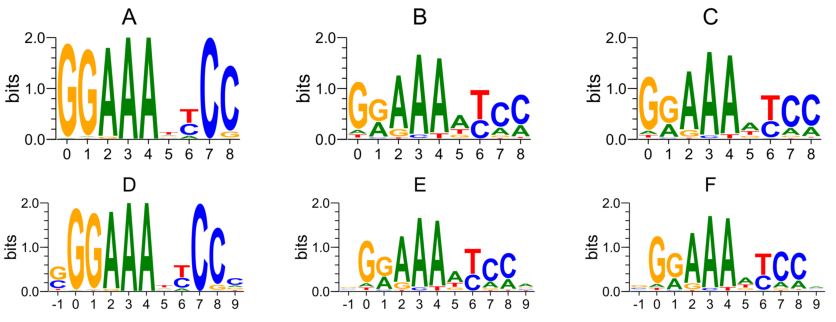
\includegraphics[width=6in]{plotCACATG302015.pdf}  %logos0_30bp.eps}
\caption{Logos generated for known Dorsal sites tested for adjacency to 5'-CACATG used as 'cooperative' class (DC) if in the [0,30]bp distance.  Logo A corresponds to the 'Dorsal Cooperative' class, it's total information content we calculated at 13.4bits.  Logo D is the exact same logo as A but we've appended one base-pair of flanking sequence onto the start and end of the site (hence, this logo starts at position -1).  Position 9 of this logo shows about a couple decibits of information relative to the background sequence and the position -1 contains a half bit of information.  Logo B is the 'Dorsal Uncooperative' class for the [0,30]bp window, which we calculated to have 9.4 bits information relative to the background (uniform distribution of bases), and logo E has added the flanking sites to the 'Dorsal Uncooperative' class.  Logo C is the CB motif with 9.7 bits of information relative to the background, which looks similar to the 'Dorsal Uncooperative' class at position 6 due to there being many more sites that prefer A to a T at this position amongst all the Dorsal sites in the network.  Logo F is the CB motif with the flanking sequence appended.}
\end{figure}

\par


  \begin{tabular}[b]{|c|c|c|c|}
\hline
spacer   &  [0,30]bp & (31,60]bp &(61,90]bp  \\ \hline
\multirow{2}{*}{}  Mutual Information \Eref{mi}&  0.38 & 0.28 & 0.04  \\
 Logodds ratio test -log(p value)& 4.8 & 0.17 & 0.66 \\
\hline
\end{tabular}\label{tablesuple}

\par

The  table \ref{tablesuple} second row corresponds to the log odds ratio test based on CB's specificity set at $10^{-4}$, which corresponds to a CB energy of 2.5, as in the main text.  The DC detector did show better performance for this spacer window and corresponding energy cutoff.  We additionally ananlyzed the mutual information for the case that 5'-CACATGT was used as a motif for Twist, which would correspond to a subset of the sites found for 5'-CACATG.  For the 5'-CACATGT motif we found the mutual information was 0.3, 0.17, 0.0 for the three possible cases of the sliding window.

\newpage

\subsection{ROC curve}
 The ROC curve for the OR gate and the CB detector for 5'-CACATG Twist motif are displayed in \Fref{rocfig2sup}.  The detectors behave similar to the results presented in the main paper for the 5'-CAYATG motif.
\begin{figure}[!htbp]
\includegraphics[width=5in]{rocenhaCACATG30.eps}
\caption{ROC curves display the False positive rate (FPR) vs. True Positive Rate (TPR).  }
\end{figure}\label{rocfig2sup}


\newpage

\subsection{ Mutual Information between loci classes $C$ and detector predictions of classes $P$}
The mutual information $I(C;\mathcal P)$ for both conditional detectors based on a 5'-CACATG Twist motifs in \Fref{miCPsup} shows similar behavior as the results in the main paper for the 5'-CAYATG Twist motif.   
\begin{figure}[!htbp]
\includegraphics[width=5in]{miclassesCACATG30.eps}
\caption{The mutual information $I(C;\mathcal P)$ between the conditional detector's prediction's of class types (distal or proximal) and the known class types, as a function of the detection energy threshold is varied.  DC shows about .3 bits of information at about an energy cutoff of 4.  DU does performance suggests not much better than random guessing for its predicting class types.  }
\end{figure}\label{miCPsup}

\newpage
\subsection{Permutation test using ranksum statistic } 

The median energy of DC was 0.4, and the median energy of DU was 2.9.  The plot of the ranksum sampling distribution generated from random partitions of these data sets of size 66 and 356 respectively is below.
\begin{figure}[!htbp]
 \includegraphics[width=5in]{rsCACATG30.eps}\\
  \caption{ Histogram of p-values of random partitions of the combined data set $\mathcal D_{\textbf{CB}}$, where the histogram bins were in units of 10*log(p value).  The p-value of the ranksum test for DC and DU median energies was about 205 in the scaled log units, which is the bar at the far left of the sampling distribution. }
\end{figure}\label{bb}
\newpage
\subsection*{Propagation of error for estimating error in Entropy estimates }
Initially we conflated our notation of the frequency of events $i$ from an alignment with the theoretical probability of the event $i$.  Here we must distinguish these two ideas.  Let the frequency of the event $i$ (for example the occurrence of the symbol or nucleotide 'A') be $f_i$, and the probability be $p_i$ (previously denoted as $P(B_i)$, which we will abandon since it is too cumbersome here).  What is the standard deviation of an entropy estimate?  One way to estimate this is resampling (bootstrap).  Another, much simpler technique is to treat the entropy as a function of a variable, and then simply see how much a variation of the variable (of some specified size) causes variation in the function.  Here the idea is to treat the input variation as "error" and see how much this affects the output.  
Here "error" means uncertainty which is reliably estimated as the statistical standard deviation of the variable (if this is known), or can be estimated by any justifiable means (e.g. the error in a measuring device, is reasonably estimated by the resolution of the device, which is the distance between tick marks on a ruler).  

Let the true entropy be $H(p)$, which we estimate by $H(f)=-\sum_i f_i\log(f_i) =\sum_i h(f_i)$, where $h(f_i)=-f_i\log{f_i}$.  We wish to estimate the error in this estimate (the standard deviation of $H(f)$), which can be estimated using the formula:

\begin{equation}
\sigma_{H(f)} = \sum_i \frac{\partial{h(f_i)}}{\partial{f_i}} \sigma_{f_i},
\end{equation}
This formula assumes that our estimate of uncertainty in $f_i$ is $\partial f_i$, which is equivalent to the standard deviation of $f_i$, where, for example\footnote{Recall for Poisson processes the variance is equal to the mean for the counts.  Hence, $< (n_i - Np_i)> = < n_i > =Np_i$.  Also recall that the variance of a random variable scaled by a constant, for example $1/N$, is $var(X/N) = var(X)/N^2$.  Therefore the variance in the frequencies $f_i$ is $\sigma_{f_i}^2= \frac{p_i}{N}$}, the expected standard deviation of $f_i$ for a Poisson process is $\sqrt{p_i/N}$.
\begin{equation}
\frac{\partial{h(f_i)}}{\partial{f_i}} = -(\log{f_i} +1 ),
\end{equation}
where we know the derivative of $log(x)$ with respect to $x$ is $-1/x$, and we used the product rule of differentiation on the term $f_i \log{f_i}$.  Using the above computation we can now see how a variation in magnitude equal to a standard deviation of the frequency of event $i$ will contribute to the error (the standard deviation) in the entropy\footnote{What is the point of doing propagation of errors?  Well, it's reasonable to assume a repeated counting experiment will arrive at a different value of $f$ for each experiment;  hence, within the statistical estimate of the standard deviation, which is $f(f-f)$ for a Bernoulli process, we would like to know how much this variation will cause variation in the entropy.}.

Now the propagated error to the entropy is:
\begin{equation}
\sigma_{H(f)} = |\sum_i \frac{\partial{h(f_i)}}{\partial{f_i}}| \sigma_{f_i}, 
\end{equation}
  \begin{equation}
\sigma_{H(f)} = |\sum_i-(\log{f_i} +1 ) | \sigma_{f_i},
\end{equation}
  Now we simply must declare the type of measurement process on $f_i$.  If we assume a poisson process, then plugging in to the above formula for the standard deviation $\sigma_{f_i}$ we have\footnote{Any information theoretic quantity can be converted to an entropy using standard identities.  Hence, for example, the information content of a binding site logo is $IC = H_{max} - H(P(S))$, where P(S) is the PWM estimate of the binding site sequence distribution.  The error in this estimate is approximately just the additive error in the two entropy terms.  The maximum entropy is known with certainty and hence has error zero.  Hence, the information content error of a PWM is simply the error estimate of the binding site sequence distribution's entropy. }:
    \begin{equation}
\sigma_{H(f)} = |\sum_i -(\log{f_i} +1 ) | \sqrt{\frac{p_i}{N}},
\end{equation}
\begin{figure}[!htbp]
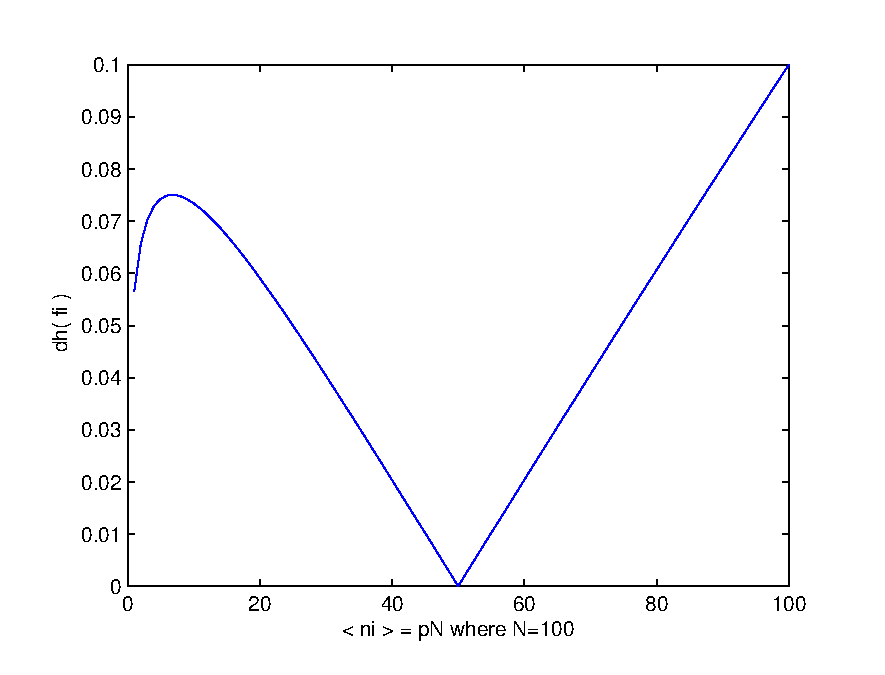
\includegraphics[width=5in]{entropyN100}
\caption{The estimate of the error, $dh(f_i) = \sigma_{h(f_i)}$ is plotted on the vertical axis, when the number of counts of event i occur at their expected value, where the horizontal axis is the expected number of counts observed for event i, $< n_i >= p N$.  }
\end{figure}\label{entropyerr}
\subsection*{Determining if differences in Information are significant}

From figure \ref{entropyerr} we see that we need, in the worst case scenario, about 4 decibits (about 4*.1 bits, which was the maximum value in the graph) of information content to biologically distinguish two alignments each of 100 binding sites of DNA (i.e. in order to distinguish two columns of a PWM).  However, the standard error of the entropy requires dividing the estimated variance by N, in which case, two alignments are statistically resolvable ('significantly different') if they are different by .4 centibits, which may or may not be biologically significant.  What is biologically significant?  For example, can natural selection resolve binding sites that have differences in information scores of .4 centibits?  Depends on the selection pressure, and how big it is.  Certainly selection can resolve .4 centibits, given drift doesn't cause the variation in the population to disappear.  What is physically different?  For example, can Dorsal protein resolve binding sites that are different by .4 centibits?  Well, given that Dorsal can sample binding sites, then given $2^{H(P(S))}$ binding events, we would expect a Dorsal to correctly identify a binding site relative to the background of the genome (where $P(S)$) is the PWM probability).  So in a statistical sense, yes it seems to be physically significant, since .4 centibits can reduce the amount of sampling required.  In fact, any information that Dorsal has about its binding site sequences is physically significant due to this idea\footnote{This doesn't mean all binding site sequences with information scores greater than zero are functional (adaptations) in Eukaryotes, as Schneider found for prokaryotes\cite{pmid3525846}.}  

%It means that Dorsal protein, using a PWM detector, has information about the symbolic content (its base-pair preferences) of the functional sequences (e.g. the few bindings site loci's sequences that Dorsal targets).}.   

\subsection*{Entropy Bias from Maximum likelihood estimation}
The estimate of the error (standard deviation\footnote{this is not a 'standard error'}) in the entropy in the above section was based on estimates of the frequencies $f$.  The estimates of the frequencies were based on Maximum Likelihood  Principle, which is unbiased for frequency estimates.  

Functions of known unbiased estimates (such as the frequencies) are not necessarily unbiased (such as the entropy).  It is known that the entropy estimate is biased if one uses ML estimates for their frequencies.  To see this we can Taylor expand the above estimator $H(f)$ about the expected value of $f$, which is $p$ (there's no bias in the expected value of $f$).  Using the same notation as Bialek (see page 547 \cite{bialek}, we will first add and subtract the expected frequencies from each factor:
\begin{equation}
H(f)=-\sum_{i=1}^4 (p_i+\delta f_i)\log(p_i + \delta f_i)
\end{equation}
 where $\delta f_i \approx \sigma_{f_i}$ in my notation above, and since we're expanding about the 'expected value' we have $\delta f_i= (f_i - p_i)$ (plugging that into the equation you see we've just written the definition of the entropy).  Now Taylor expanding (where recall, the expansion of $log(1+x) = -x$) we have:
 \be
H(f)&=-\sum_i p_i \log{p_i} -\sum_i(\log{p_i} + \frac{1}{ln(2)}\delta f_i) ) \\
 &- \frac{1}{2}\sum_{i=1}^4 \frac{1}{ln(2)p_i}(\partial{f_i})^2 + \epsilon \\
\ee{equation}
here the last term in the expansion is the error term (capturing higher order terms), and expression $(\partial{f_i})^2 $ acts as the variance $(\partial{f_i})^2 = \sigma_{f_i}^2$ in my notation in the section of entropy propagation of errors.  The variance term is the average squared fluctuation, the standard deviation squared, which is a positive number (even if any given fluctuation is negative).  Now, we can take the expectation value of the Taylor expansion, and of course, the fluctuations are just as likely positive as negative, and they'll cancel (or just recall that $f_i=p_i$).  The first term in the expansion above is a constant (it's the true entropy).  Hence we find something a bit odd, the expected entropy is not the true entropy!  This is a bias.  The expected entropy, to second order is:
 \be
H(f)&=-\sum_i p_i \log{p_i}  - \frac{1}{2}\sum_{i=1}^4 \frac{1}{ln(2)p_i}(\partial{f_i})^2 + ...  \\
\ee

Maximum likelihood estimates of the entropy underestimate the true entropy.  Why?  Well mathematically, the second term on the right side of the equal sign is assumed to be dominant over other higher order terms (where we're assuming this expansion converges).  The second term contains the variance (a positive quantity).  The true entropy (first term on the right side) is always positive or zero, hence subtracting the \emph{smaller} variance term from the true entropy leads to an underestimate of the true entropy (always).   

To estimate the bias in the entropy we must compute $< H(f) > - H(p) $, which as seen above can be estimated by $\frac{1}{2}\sum_{i=1}^4 \frac{1}{ln(2)p_i}(\partial{f_i})^2  = \frac{1}{2}\sum_{i=1}^4 \frac{1}{ln(2)p_i}\sigma_{f_i}^2$, where we have substituted in the standard variance symbol for the squared fluctuation.  Now we know the variance of a poisson process, hence plugging into the term in the last sentence for the variance we have $\frac{1}{2}\sum_{i=1}^4 \frac{1}{ln(2)p_i}\sqrt{pi/N} =\frac{1}{2}\sum_{i=1}^4 \frac{1}{ln(2)}\sqrt{1/N}$.  Hence, we see for DNA nucleotide counts, the entropy at a given site is biased by $2\frac{ln(2)}{ln(2)N}$.  For small sample size (small N) this can have a large effect, even larger than the estimate of the variance itself $\sigma_{H_{f}}^2$.  
\subsection{Entropy Bias}\label{entro}
Changing notation, we now will simply conflate the estimates of frequencies $f$ with the true probability $P$.  The Bayesian estimate of the probability of $B$ with a Dirichlet prior using symmetric hyperparameter $\beta$  is $P(B)=\frac{n_{B}+\beta}{N+4*\beta}$\cite{MEP}.  Unlike the ML estimate of entropy (which underestimated the entropy) this particular choice of hyperparameter is known to be an overestimate of the true entropy.  Hence, in Beyesian estimation, it is possible for the small sample bias to be either over or under the true value.  For example, the Baysesian estimate approaches the ML estimate as we let $\beta$ approach zero, which can be seen in figure \ref{entropybias}.  This is expected since if $\beta$ is zero we then have:  $P(B)=\frac{n_{B}+\beta}{N+4*\beta}=\frac{n_{B}}{N}$.

To minimize the bias in the entropy we selected the value of $\beta$ that gave the smallest bias for the small sample regime.  Of course, we do not know the true entropy a-priori of the binding site distribution.  However, for the length 9 bp CB distribution of Dorsal binding site sequences we could initially estimate a 'known' PWM that could then be used to randomly generate synthetic binding sites.  Hence, using our best estimate of the CB PWM, we used the PWM to generate data sets of N binding sites.  For each synthetic data we estimated a PWM with a predefined value of $\beta$, and thereby estimated the entropy as a function of N.  For each value of N, we generated n replicate data sets, building a PWM for each set, thereby obtaining n estimates of the entropy for each value of N.  We estimated the entropy based on a data sets of size N=[1,50], and $n=20$.  By repeating this experiment for values of $\beta$ in the domain $[10^{-5},0.1,0.2,0.25,0.5, 1]$ we found an empirical value of $\beta$ that best estimated the 'known' entropy and energy.  We similarly repeated this for energy estimates, and found the least biased vale of $\beta=0.1$ for entropy and energy estimates.
\begin{figure}[!htbp]
\label{entropybias}
\includegraphics[width=5in]{EntropyBiasCB_L9.eps}
\caption{ The probability distribution p was estimated from N random deviates of a 'known' length 9 PWM that was built from $D_\textbf{CB}$ data.  The entropy of p, $H[p]=-\prod_{i=1}^9 \sum_B p(i,B) \log p(i,B)$ , where $i$ runs over the nine positions of the aligned N sequence deviates, and $B$ runs over the bases, was computed for twenty replicates for each value of N and plotted the average entropy over the twenty replicates as a function of N.  We computed the functional H as a function of N for values of $\beta$ in the domain $[10^{-5},0.1,0.2,0.25,0.5, 1]$.  The 'known' CB PWM had an entropy of 5.6 bits as observed by the green horizontal line, and found an empirical value of $\beta$ that best estimated this 'known' entropy to be $\beta=.1$ as shown by the red plot of the functional H as a function of N.  We similarly repeated this for the functional energy estimates, and found the least biased vale of $\beta=0.1$ for entropy and energy estimates.}
\end{figure}




\newpage
\chapter{}

%\input{introchap3}


 \section{Model Background}

 \subsection{Fractional Occupancy of Morphogen Binding to DNA binding Site}

The binding process is modeled using a first order rate law, where M is morphogen and B is the Binding site of DNA, and MB is the complex:
\begin{equation}\label{}
    \frac{d [MB)]}{dt}= k_{on}[M][B] - k_{off}[MB],
\end{equation}
where the brackets [ ] denote concentrations, and $k_{on}$ is diffusion limited on rate,  and $k_{off}$ is the off rate that is determined by the electrostatic interactions and will vary between morphogens.  Using chemical reaction notation, we can write the above rate law as:
\begin{equation}\label{}
    [M] + [B] \Leftrightarrow [MB].
\end{equation}
In equilibrium we have:
\begin{equation}\label{ka}
  K_{a} =  \frac{[MB]}{[M][B]}= \frac{k_{on} }{k_{off}},
\end{equation}
where the $K_{a}$ is the association constant (binding constant).
The Binding site is either occupied ($o$) or unoccupied ($u$) hence the total ($t$) amount of B is conserved :
\begin{equation}\label{}
    B_{t} = B_{u} + B_{o}
\end{equation}
From this equation one is able to construct a Binomial probability space\footnote[2]{If we encode the bound state and unbound state in the Bernoulli Random variable (i.e. 1,0) we have: $E(X) = \mu = \sum_i X_i P_i = 1 P + 0 (1-P) $} \footnote[3]{ $\sigma^2 (X) =\sum_i (X_i-\mu)^2 P_i = (1-P)^2P + (0-P)^2(1-P) = (1-P)P $ }.  The fraction of occupied binding site $B$ determines the distribution's parameter $P$:
\begin{equation}\label{}
   P = \frac{B_{o}}{B_{t}}
\end{equation}
which can be rearranged in terms of the concentrations (i.e. [MB] and [B]):
\begin{equation}\label{Zb}
    \frac{B_{o}}{B_{t}} =\frac{[MB]}{[MB] + [B]}
\end{equation}

\begin{equation}\label{}
    P =\frac{[MB]}{[MB] + [B]} = \frac{K_{a}[M]}{1+K_{a}[M]}.
\end{equation}
Again, $K_a$ is the association constant of the morphogen, $M$, to the binding site $B$.  Previously we have denoted this constant as $K(S)$, where $S$ is a DNA sequence that functions as a binding site for the morphogen. 

\subsection{Fractional occupancy of CRMs containing multiple binding sites }


Given that most regulatory sequences have multiple binding sites for multiple different morphogens one has a master equation governing the binding process, a set of coupled differential equations.  Here, again, we will assume the binding process has equilibrated, and hence we simply must enumerate the states (configurations of bound and unbound sites) of the many-binding site system.  For independent binding this is simply multinomial process (where the 'multi' aspect accounts for the different types of transcription factors binding to the CRM).  For example, for a single type of transcription factor binding, to n binding sites within a CRM, one has a binomial process governed by the partition function $(1+q)^n$, as discussed in the introduction of the dissertation.  Hence, the probability of k bound factors is simply $P(k) =  {n \choose k}p^k(1-p)^{n-k}$, where $p$ is a Boltzmann probability for a single bound site, and $p^k(1-p)^{n-k}$ is joint probability of a particular binding configuration (\emph{which} configuration is irrelevant for the case of identical sites binding the same morphogen).  However, for the case of dependencies between the sites, we can not factorize the joint distribution over binding sites (\textit{i.e.} $(1+q)^n$ is a factorization of the partition function, and hence factorization of the joint distribution).  Furthermore, for the case where the sites are not identical, such as in CRMs that have heterogenous binding sites due to each transcription factor's DNA sequence specificity, we do not simply have one Boltzmann probability $p$ for all the sites.  Hence, each site will need a distinguishing notation.  Furthermore, the number of sites $n$ is not always known.  Hence, in some cases, one must discover $n$ sites, by 'annotating' the CRM which defines the coordinates of each transcription factor's sites and their corresponding energy.  In the next three sections we will describe a notation that is a mixture of notations used for Hidden Markov Models (HMM) and Lattice Gases (Ising Models) that is hybridization of the notations from Segal et.al.\cite{pmid18172436} (HMM notation) and the notation used by both Xin He et.al.\cite{pmid20862354}\cite{pmid19956545}.  Hereafter these notations will simply be referred to as Segal's notation or Xin's notation.  The reason for the hybridization is because our model was originally based on the Segal's paper, which latter was merged with work from Xin He (who collaborated with others in Saurabh Sinha's lab and S. Zhong's lab), by usng Xin's GEMSTAT and STAP C++ programs as libraries for implementation of our model.

\subsection{Segal's Hidden Markov Model}     

 If one does not know the binding sites \textit{a priori} of a CRM then one could take all possible positions within the sequence as the start of a new binding site as in figure \ref{sb}, where the PWM (see chapter 2) scores each position of the sequence as a potential binding site, thereby creating a list of binding energies ordered according to the position within the CRM.  Repeating this for each morphogen's PWM, and by stacking the lists on top of each other, results in a matrix of energy scores that is useful for computation of the partition function through the forward algorithm from Hidden Markov Models (HMMs).  
 
 The partition function of the many body system requires the addition of the statistical weight (see the Boltzmann factor in equation \ref{wc}) from each possible 'path' through the matrix.  Each 'path' through the matrix represents a 'configuration' as in figure \ref{configurationMatrixI}.
\begin{figure}
  % Requires \usepackage{graphicx}
  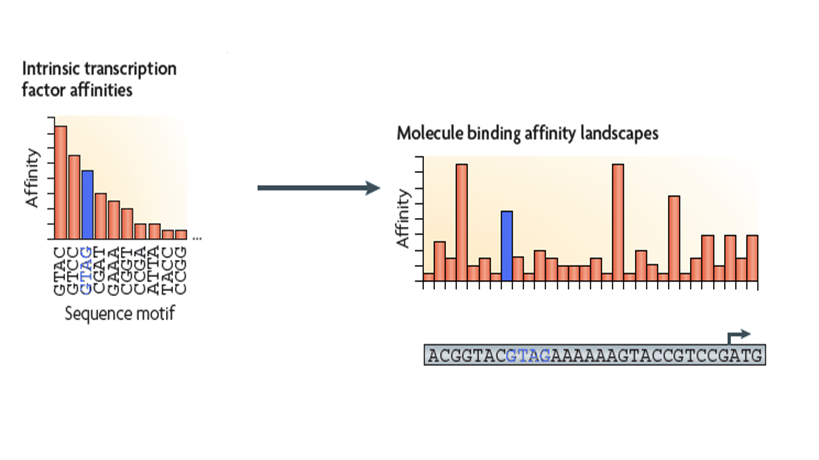
\includegraphics[width=1\textwidth]{segalblandscape}\\
  \caption{Widom, Segal Nature Review Genetics; "motif" denotes path through the PWM\cite{pmid19506578}}\label{sb}
\end{figure}
The partition function can be calculated by recursively moving through the matrix elements, in a way that is similar in spirit to standard algorithms of multiple sequence alignment\cite{BSA}, where we can think of each configuration as a possible way to 'align' each motif (PWM) to the CRM.  The variant of HMM's forward algorithm approach used by Segal for computing the partition function of all paths (configurations) is discussed in his supplementary material. 
\subsection{Enumerating the configurations of a CRM sequence }

 Here we will introduce a notation for the weights of many-binding site systems.  First, let $P(c)$, be the probability of a particular configuration (c) occurring
\begin{equation}\label{mbody}
    P(c) = \frac{W(c)}{\Sigma_c W(c)},
\end{equation}
where $ W(c)$ is the boltzmann factor or weight of the binding configuration, which is a list of occupations for each binding site locus within the CRM, where the occupation is either bound or unbound.   Using the notation of Xin, from Sinha lab ( which was using Buchler's model as a guide\cite{pmid20862354}\cite{pmid12702751}, a notation used by Terrell Hill that I followed in the Introduction of the Dissertation), we have:
\begin{equation}\label{wc}
    W(c)=  [\prod_i^N q(x)_{tf(i)} ] [\prod_{j}^{N-1} \omega_{tf(i),tf(j)}(d)]
\end{equation}
Here we have $N$ bound transcription factors, where $q(x)_{tf(i)}$ is the weight of the transcription factor for the ith binding site ($tf(i)$) that is $\textbf{bound}$ at position $x$ of the sequence, 
\begin{equation}\label{partitionf}
    q(x)_{tf(i)} = K_{s(x)}^{tf(i)} [tf(i)]
\end{equation}
Here $ K_{s(x)}^{tf{i}}$ is the equilibrium constant $K_a$ from equation \eqref{ka} for the binding site sequence $s$ binding by transcription factor $i$.  And $\omega_{i,j}$ is the interaction between the two $\textbf{bound}$ factors $tf(i),tf(j)$, where we have one less nearest neighbor interaction than the number of bound factors.  And $d$ is the distance separating factor $tf(i)$ from factor $tf(j)$ in units of base pairs ( $d = x(tf(i)) - x(tf(j))$ where $x(tf(i))$ is the sequence coordinate of factor $tf(i)$).
\subsection{The configuration vector nomenclature}

 Here we have used 'c' to denote the binding configuration of bound and unbound factors on the CRM following the symbol Segal used to denote the configuration, and we have used a map $tf(i)$ to link each binding site i to a transcription factor.  This map is similar to notation used by Segal, where he explicitly denotes the type of transcription factor at each bound site.
 
  Xin used a configuration vector, $\sigma$, which had indicator variables $\sigma_i$ for ith componenet of their configuration vector, where the ith component was the ith binding 'site'.  Xin's notation is elegant, in that every 'site' in their model is clearly represented in their configuration vector by the occupancy of the ith component of the vector.  
  
  Segal's notation does not display all the possible bound and unbound positions in the configuration (since there is a background occupancy in his model that causes unbound sequence to have a Boltzmann weight of 1.).  I have tried to stick to Segal's notation for a configuration by only displaying bound factors in the Boltzmann weight of a configuration, and by denoting explicitly the type of transcription factor at each bound site.  However, Segal's notation is based only on the CRM sequence, he does not actually have a 'site' notation, since every possible position in the CRM is considered a binding site for each transcription factor, and he simply looks at all the possible ways that coordinately regulating transcription factors could form monolayers on the CRM, without overlapping one another.  Hence, in Segal's notation, there really is no notion of a 'functional' site, as each \textit{possible} position within the CRM is a place for the factor to 'plant' itself (a place for the transcription factor to bind), where \textit{possible} is distinct from \textit{probable} by the use of PWMs.   
   
Seeing that binding sites are 'functional' (adaptations), or at least vestigals or exaptations, the notation of Xin for defining a 'site' we have tried to hybrid with Segal's notation.  Xin's notation is fundamentally based on binding 'sites' (adaptations).  For example, by either setting a threshold on a PWM to discover sites, or by knowing \textit{a priori} what are the binding 'sites' (regulatory adaptations), Xin starts the configuration problem (the notation) with N binding sites.  The indicator variables of the configuration vector are equivalent to occupancy of each site, hence $\sigma_i$ is either 0 or 1 for each component of the configuration vector.  For example:
\begin{eqnarray}
W(c)=W(\sigma)&=& W(\sigma_1,...,\sigma_{N} , \sigma_{1,1},..,\sigma_{N,N})\\
&=& \exp{(-\sum_i^N ln(q_i) \sigma_i - \sum_j^N ln(\omega_{ij}) \sigma_{ij})}
\end{eqnarray}
% \begin{equation}\label{}
%    W(c)=W(\sigma)= W(\sigma_1,...,\sigma_{N} , \sigma_{1,1},..,\sigma_{N,N}),
%\end{equation}
Here, $ln(q_i)$, is the free energy of binding to the $i$th site, and $\sigma_{i}$, denotes the occupancy of the $i$th 'site', and $\sigma_{ij}$ denotes the pairwise energetic interaction $ln(\omega_{ij})$ between site $i$ and site $j$\footnote{Recall for the canonical ensemble, where H is the Hamiltonian of a configuration we would have  $W(c) = \exp{-H(c)/kT}$ being a simple Boltzmann factor, where k$T$ is the thermal energy.  We are working in a grand canonical ensemble, which allows for particle energy as well as energy exchange, hence, the total energy of the configuration is a function of the Hamiltonian and the chemical potential of the factors, which causes concentration of the transcription factors to influence the total energy of a configuration, hence the energy is a thermodynamic free energy}.  But what type of transcription factor is binding to the $i$th site?  In Xin's notation, this is not decipherable.  Rather, in their notation, each 'site' corresponds to a particular factor.  But we simply don't know which factor.  Hence in Xin's notation it's possible that two distinct 'sites' occupy the exact same locus.  Hence we don't know if two sites are overlapping.  Overlapping sites can not both be bound, since all thermodynamic model's for occupancy of transcription factors use 'hard sphere potentials', there's steric hinderance prohibiting two transcription factors to occupy the same space along the CRM.).  Hence, in Xin's notation, one is supposed to be cognizant that bound overlapping sites will set that configuration's weight to zero. 

We have used a hybrid notation in Eq.\ref{wc}, where it's not that our CRM has N fixed binding sites (like in Xin's notation) that are each bound or unbound.  Rather, the weight $W(c)$ displays $N$ bound sites from a configuration c.  Hence, in our notation $N$ is a variable in the binding configuration space, while in Xin's notation, N is the fixed number of sites.  In Xin's notation, advantageously, they can put a bound on configuration space as $2^N$, this is an upper bound because overlapping sites will reduce the total number of configurations, furthermore this overcounts the number of unbound states, since a loci's sequence that match for multiple factors - say m factors- would consider $2^m/2-1$ too many configurations, since the loci is actually only unbound in one possible way\footnote{Xin's GEMSTAT computes the correct weights and partition function, it's just the estimate on the configuration space that is a bound.}.   
\subsection{An example of the hybrid configuration notation} 
For an example of the hybrid notation, consider all possible positions of the CRM as a binding site, as Segal would, and multiple morphogens binding to the same site ( same position within the sequence, same locus ); then the configuration vector (c) can be written in terms of Xin's indicator variables (similar to Ising models).  
 
For a length L CRM and for 3 transcription factor types (like Dorsal,Twist, and Snail) we have in Xin's notation $N =4*L$, where the factor of four is due to the four types of transcription factors at each locus - namely: bound by Dorsal, Twist, or Snail or 'background' (background is a type of pseudoparticle that fills the unbound state)).\footnote{As pointed out by Segal in his supplement, this problem may seem computationally infeasible, since the number of configurations for L=500 is of size $2^{4*500}$, but due to the forward algorithm it is possible.  Here the number of binding sites, $N$, neglects edge effects of k-mers requiring length k binding site sequences.  Hence, the calculation of the number of configurations is only a bound on the cardinaility of the set of configurations, where the bound is further affected by the neglect of overlapping sites that cause many configurations to be unaccessible (against the rules). } 

In this case, the vector of indicator variables is written as a matrix of size 4xL.  For example, for the toy CRM sequence 'acggt', we would have a configuration vector of size 20.  If we add another 'state' to the configuration vector denoted as 'silent' to represent steric effects, where the type of transcription factor indicator variable now only indicates the 'start' of a binding site, we would then have a indicator matrix of size 25, as indicated in Figure \ref{configurationMatrixI}, where the Dorsal transcription factor occupies positions 2 and 3 of the CRM (in this toy case Dorsal occupies a site just of length 2), and the rest of the CRM is occupied by the background factor.  Hence the configuration vector (a value of the matrix of indicator variables) is of size N+5 (the 5  due to the 'silent' states) assuming no interactions between bound factors.  If there are interactions, for example nearest neighbors, then there are an additional $\frac{16N^2}{2}$ components to the configuration vector, which we will not display.
 
\begin{figure}
  % Requires \usepackage{graphicx}
  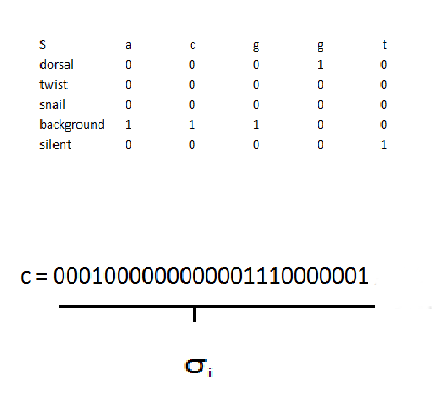
\includegraphics[width=1\textwidth]{configurationMatrixIb}\\
  \caption{The toy CRM sequence acggt is annotated at each of its loci ( positions ) to denote the configuration vector in row major ordering (1st five bits are dorsal's row, second five bits are twist's row etc...).  In the language of HMMs, the value of a configuration vector reveals the hidden state of the sequence.  Here there are 5 states, where the 'silent' state indicates a transcription factor is bound to an upstream position of the sequence, causing the loci to be covered by an internal position of the planted factor.  }\label{configurationMatrixI}
\end{figure}

Now that we have defined our configuration notation, and described the weight of a given configuration, we will explain in the next section our novel form of the pairwise interaction $\omega$ between bound factors.
%
%\begin{figure}
%  % Requires \usepackage{graphicx}
%  \includegraphics[width=1\textwidth]{1042015/HMM}\\
%  \caption{}\label{HMM}
%\end{figure}
%
%\begin{figure}
%  % Requires \usepackage{graphicx}
%  \includegraphics[width=1\textwidth]{"1042015/configuration"}\\
%  \caption{configuration or many-body state of the system}\label{configuration}
%\end{figure}

%%%%%%%%%%%%%%%%%%%%%%%%%%%%%%%%%%%%55ab

\subsection{The pairwise interaction $\omega$ between bound factors}
%
Transcription factors often interact with each other, causing certain configurations to be more likely by decreasing the total energy of the configurations where interacting factors are jointly bound, thereby increasing the weight of those configurations.  This observation, was the physical basis behind A. Hill's famous Hemoglobin Oxygen binding model.  

In the work of Xin a number forms of distance dependent pairwise interactions between bound factors was tested, such as sinusoidal functions over space that account for 'phasing' where one bound factor interacts with the nearest neighbor that is in phase (by using the major groove distance) with the factor of interest.  Similarly, gaussian decays from the center of the planted factor, and square functions were attemted and implemented.  Hence, GEMSTAT has a small database of pariwise interaction forms.  All the forms, as ours too, only allow for interactions between nearest neighbor bound proteins. 

For the the DV network interactions between Dorsal and Twist have been experimentally shown to be distance dependent, hence we use an interaction that is a function of the DNA basepair distance separating the nearest neighbors.  For the network that we are modeling this distance dependent interaction has been shown to be dominant force driving the Dorsal border of neuroectoderm expressed genes.  For the neuroectoderm network\footnote[2]{neuroectoderm network are the set of genes coordinately expressed in the lateral regions of the developing embryo, this developing tissue spans about 10 cells at the time point under consideration}  Crocker et.al. and Szymanski et.al. \cite{pmid7774581},\cite{pmid18986212}have shown that the spacing between sites plays a dominant role in defining the number of cells that are turned on in this region (width or span of cells).

For both the DV and AP (Anterior Posterior) network short range antagonistic interactions have been show to dominate the action of repressor transcription factors\cite{pmid20087339}.  The Snail transcription factor is a short range repressor acting to regulate the DV axis, which we also model using a distance dependent interaction, commonly called 'Quenching'\cite{pmid20087339}.
\begin{figure}
  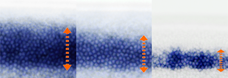
\includegraphics[width=1\textwidth]{rhoNEEs}\\
  \caption{ Changing the spacing between motifs in modules change the span of cells that are expressed.  In this Figure the spacing between two sites was adjusted by Natural Selection in orthologs of the \textit{rhomboid} gene's CRM. When the ortholog CRMs were transgenically inserted into \textit{mel} species the width of the expression pattern changes relative to the endogenous pattern width, suggesting that coopertivity between the sites is a function of the distance between sites that can be used by evolution to 'fine tune' the epression patterns in development.  When each sequence or module is expressed in its respective specie (lineage), then the relative widths (w/L where L is the lengths of the major axis of the specie's embryo, w is the width of the tissue in nanometers that express the gene) of the tissues are the same.  Different specie's embryos have different sizes hence there is a scaling law - how a characteristic (such as gene expression) changes with body size.  This Figure is from Erives Crocker et.al 2008 "Evolution acts on enhancer organization to fine-tune gradient threshold readouts. PLoS Biology"}\label{rhoNEEs}
\end{figure}

  Furthermore, since we do not know the exact form of the function, we bin the distance separating the proteins, and for each bin a free parameter is fit.  One may look for a coarse binning of the separation distance in bins of 10bp, or as fine as bins of 1bp.  If we choose the former option than an example of our protein-protein interaction parameter would be as follows:
\begin{equation}\label{}
   \overrightarrow{ \omega(d)} =  [ \omega_1 ,\omega_2 ,\ldots, \omega_b,\ldots,  \omega_n ]
\end{equation}
where the subscripts of the components of the $\omega$ vector (coopertivity or synergistic protein-protein interactions)  represent the corresponding bin ,b, ( in this case there are n bins), hence they define a bin vector, $\overrightarrow{B}$, where its components corresspond to the interval of base pair distances.

\begin{equation}\label{}
\begin{split}
 \overrightarrow{B}   &= [ B_1 ,B_2 ,\ldots, b, \ldots, B_n ] \\
     &=   [ (0-10), (11-20), \ldots,(41-50),\ldots, (x-L)]
    \end{split}
\end{equation}
Here bin b, is all interactions where two bound sites are separated by 41-50 basepairs, and x represents the last bin border, and L represents the Length of the module (sequence).  This representation of coopertivity vector, is really only useful for programming purposes, mathematically the coopertivity is simply a piecewise defined function:


\[
  \omega(d) =
  \begin{cases}
   \omega_1  & \text{ if } d \in (0,10)  \\
   \omega_2  & \text{ if } d \in (11,20)  \\
   \ \ \ \ \ \vdots \\
 \omega_n  & \text{if } d \geq x
  \end{cases}
\]

Our aim is to fit the biochemcial parameters that tune the probability of configurations that occur in live embryos.  However, we simply don't have such detailed biochemical experiments.  Hence, we use the mRNA of the target genes regulated by Dorsal Twist and Snail as a readout of what binding configurations are likely occurring, and wheter certain configurations have strong linkage (pairwise interactions) between certain bound factors.  Hence, we must infer from mRNA data, what is occuring at the DNA binding level; an expression to sequence model.  In the next section will describe a ubiquitous and obvious assumption, mRNA is caused by PolII, hence PolII binding is a proxy for gene expression.
 
\subsection{Relating the number of mRNA transcripts to fractional occupancy of PolII }
The amount of transcription that occurs at a gene locus is encoded in two segments of DNA sequence; first, the basal promoter that binds the Basal Transcription Apparatus (BTA), which is a massive complex of many proteins including PolII; second, and most important, the CRM that binds the morphogens or distal transcription factors (such as Dorsal) that modify and remodel the chromatin state and possibly have direct linkage with the BTA.  Hence the number of mRNA transcripts can be modeled as simply a linear relationship between the number of mRNA and the fractional occupancy of a promoter sequence (which we assume includes the CRM sequence).
\begin{equation}\label{}
     \left< N_{mRNA} \right>  \propto f_{BTA}.
\end{equation}
Of course, the occupancy of the BTA, $f_{BTA}$,  is a fraction this is at most one, hence $\left< N_{mRNA} \right> $ is the average number of mRNA molecules produced per nuclear cycle normalized by the maximum production rate over a cycle. 



 



\subsection{ Fractional occupancy of BTA }
%\begin{equation}\label{}
%     f_{BTA} = w_{0} + \sum_{m} \left< n_{m} \right>|_{t}  w_{m}
%\end{equation}
%Here  $\left< n_{m} \right>|_{t}$ is the average number of bound morphogen m, where the expectation value is over the occupation time of the morphogen m to the CRM per nuclear cycle of synthesis (similar to the time elapsed between cell divisions, but flies do not have 'cells' in early development).  $w_{0}$ is the 'y intercept' and $w_{m}$ is the 'slope'.
\begin{figure}
  % Requires \usepackage{graphicx}
  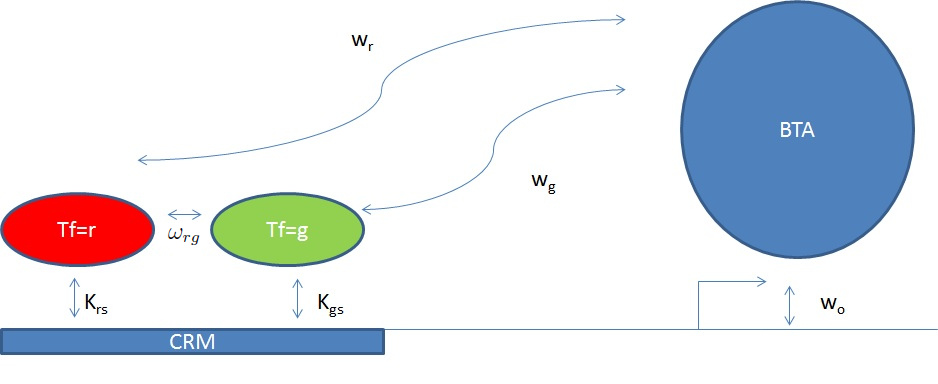
\includegraphics[width=1\textwidth]{PlugandPlay}\\
  \caption{}\label{PlugandPlay}
\end{figure}

We can gain more physical insight into the problem by thinking of mechanisms of how BTA's occupancy is a function of the morphogen occupancy.  In Figure \ref{PlugandPlay} we see that when the morphogen's are bound they have an activation or repression domain, which communicates with the BTA, for our case this communication may be thought of as the complex process of changing the epigenitic state of the chromosome, by coactivators (histone modifiers, nucleosome remodelers) binding to the morphogen.  The binding energy of this domain ($w_m$) on the mophogen can be related to the binding energy of the BTA:
\begin{equation}\label{hilldg}
     \Delta G = w_{0} + \sum_{m}  n_m(c) w_{m}
\end{equation}
Here c is a particular configuration of the morphogens on the promoter, $w_0$ is the binding energy contribution from the basal promoter, $w_m$ is the binding energy contribution from each morphogen, and $n_m(c)$ is the number of bound morphogen of species m to state c (for example see \cite{pmid19956545}).  For this configuration we could model the occupancy of the BTA as:

\begin{equation}\label{segcon}
     f_{BTA}= \frac{1}{1 + e^{ -(w_{0} + \sum_{m}  n_m(c)   w_{m}})}
\end{equation}
The fast pace timing of morphogen binding relative to transcription time (e.g. the time for PolII to clear the promoter, and a new (or preloaded on the enhancer) PolII binds), would suggest that the BTA is not sampling or cognizant of each CRM configuration of bound proteins, rather the BTA sees an average occupancy of the morphogens.  This can be modeled as:
\begin{equation}\label{segcon2}
    f_{BTA}  = 1/(1 + \exp{ -(w_{0} + \sum_{m}  \  \left< n_m \right>|_{c} \ \ \ w_{m}) }),
\end{equation}
where the occupancy of the BTA is related to the theoretical model of average morphogen m occupancy over the CRM configurations $\left< n_m \right>|_{c}$\footnote{This can also be shown, under certain conditions, to be an approximation of the much more computationally intense model of Segal et.al\cite{pmid18172436} where they compute $ \left< f_{BTA} \right>|_c = \left<  \frac{1}{1 + e^{ -(w_{0} + \sum_{m}  n_m(c)   w_{m}})} \right>|_c$.  However, as stated above, this is not an approximation of Segal's model, it's a different model of the interaction of the BTA with the CRM.}.  The average morphogen occupancy over configurations is:
\begin{equation}
   \left< n_m \right>|_{c} = \sum_c n_m(c) \frac{W(c)}{\sum_c' W(c')},
   \end{equation}   
   where we the normalized weights of each configuration are from Equation\ref{mbody}, and $n_m(c) $, is the number of morphogen of type $m$ (such as $m=Dorsal$) bound to the configuration $c$.  The expectation value is computed using GEMSTAP software from Sinha's lab, see the following reference for further details\cite{pmid19956545}.  Here after, we simply use $ \left<n_m \right>$ to denote $\left< n_m \right>|_{c} $ with the understanding that the expectation value is taken over the binding configurations of the CRM. 
%However, there is also evidence that suggests PolII is seeing each configuration, such as CCC experiments that have sequenced enhancers captured at the promoter indicating the looping model which supports each configuration of bound morphogens contributing by using a model like Segals.

% an illustration of $<n_m>$ is given in the following slides:
%\includepdf[pages=-]{gropmeet1206ina.pdf}

\subsection{ Fractional occupancy of BTA from a binding reaction perspective }
Let P = PolII concentration(this is the best known protein in the Basal Transcription Apparatus, but technically P is the concentration of the BTA), D = DNA (or basal promoter, i.e. TATA box, and binding sites for TF2B etc..), C = complex (PD).  We assume the binding process is in equilibrium (different timescale than morphogen binding).
\begin{equation}\label{}
    P + D \Leftrightarrow C
\end{equation}

Using fractional occupancy we have:
\begin{equation}\label{}
    \frac{C}{C + D} = \frac{1}{\frac{D}{C} + 1}
\end{equation}
\begin{equation}\label{}
    C = P*D*K_a
\end{equation}

\begin{equation}\label{}
   \frac{C}{C + D} = \frac{1}{\frac{D}{PDK_a} + 1} = \frac{1}{\frac{1}{PK_a} + 1}
\end{equation}
now assuming concentrations of unbound PolII is unaffected by our DNA D,we can say free PolII is a constant like 1000, and absorb the constant into the $K_a$,
\begin{equation}\label{rrr}
    \frac{1}{\frac{1}{PK_a} + 1} = \frac{1}{\frac{1}{K_a'} + 1} =\frac{1}{e^{-\frac{\Delta G}{k_bT} }+ 1}
\end{equation}
Now $\Delta G$ is the free energy that is released during morphogen binding, so  we can equate $ \Delta G $ to equation \eqref{hilldg}, however we will not say PolII 'sees' a particular configuration, rather we will assume PolII sees the average configuration (i.e. $<n_m>$ the average number of bound morphogen, m)
\begin{equation}\label{polenergy}
    \Delta G =  w_{0} + \sum_{m}  <n_m> w_{m}
\end{equation}

\begin{equation}\label{}
     <n_m> =\sum_c n_m(c) P(c)
     \end{equation}

plugging in the energy in units of $k_b T$  from equation \eqref{polenergy} into equation \eqref{rrr} we arrive again arrive at equation \eqref{segcon2}:
\begin{equation}\label{themodel}
      \frac{1}{\frac{1}{PK_a} + 1} = \frac{1}{e^{- (w_{0} + \sum_{m}  <n_m> w_{m} ) }+ 1}
\end{equation}

This yields a range of $N_{mRNA} \in [0,1]$.

\subsection{Fractional occupancy of BTA in Cooperative Binding (CB) model in Xin He's GEMSTAT}

The fractional occupancy in Xin He's Cooperative Binding model (CB) is closely analogous to our form of the model\footnote{This CB is not our related to our CB PWM model from chapter 2.}.  This can be seen by taking the simple system of one morphogen binding site with one basal promoter site for the BTA.  Hence, the BTA is treated as if it were simply another morphogen.  In this case the partition function of the two site system ($\Xi$) for the case that the two sites are independent is: $\Xi=(1+q)(1+q_{BTA})$, where q is the canonical partition function of the morphogen bound to its site and $q_{BTA}$ is the canonical partition function of the BTA bound to its promoter.  Now if we assume the sites are dependent, then we can not factorize the joint partition function\footnote{As always, we can \emph{organize} the states over our many-body system by systematically building the configurations, even in the case of dependencies, through a polynomial expansion over binding sites, which is presented in Xin He's Supplementary Material and T.Hill's text\cite{hill}.} and we then have $\Xi=(1+q+ q_{BTA} +q_{BTA} \ q \ w_{tf}) = Z_{off} + Z_{on}$, where we have collected similar terms in the expansion, where $Z_{off}=1+q$ is the term that does not include BTA binding, and $Z_off$ is the collection of the remaining terms (where BTA is bound)\footnote{In Xin's Supplement, $w_{tf}$ is denoted as $\alpha$ (which is a different parameter than our $\alpha$ that approximates the morphogen binding constant, where we choose the symbol $\alpha$ to mimic Segal's choice of parameters) $w_{tf}$ is the cooperative binding between the morphogen and the BTA}.  In their CB model they have $f_{BTA}=\frac{Z_{on}}{Z_{off}+Z_{on}}=\frac{1}{Z_{off}/Z_{on}+1}$.  By equating this to our form of the occupancy (Eq.\ref{themodel}) we have:
\begin{equation}
Z_{off}/Z_{on} = \exp{-w_o + \sum_{tf} w_{tf} < n >_{tf} }.
\end{equation}
The above equation is the odds \emph{for} BTA binding, hence the log odds is:
\begin{equation}
\ln{Z_{off}/Z_{on}} = -w_o + \sum_{tf} w_{tf} < n >_{tf} .
\end{equation}
Now, if we assume there is only one morphogen binding site, then the denominator of $< n >_{tf} $ is $Z_{off}$, and its numerator is q.  Hence we have:
\begin{equation}
\ln{\frac{(1+q)}{(q_{BTA} +q_{BTA} \ q \ w_{tf}')}} = -w_o +  w_{tf}\frac{q}{1+q},
\end{equation}
where we have replaced the Z's with their original q's and the $w_{tf}'$ denotes Xin's form of the cooperativity between BTA and morphogen (in order to distinguish from our cooperativity's symbol $w_{tf}$.  Using the properties of logarithms we can isolate $(1+q w_{tf}')$ from the left side of the equation, which leads to:
\begin{equation}
\ln{(1+q)} - \ln{q_{BTA}} - \ln{(1+qw_{tf}')} = -w_o +  w_{tf}\frac{q}{1+q},
\end{equation}
where $w_o$ is $\ln{q_{BTA}}$ leaving the result:
\begin{equation}
\ln{(1+q)} - \ln{(1+qw_{tf}')}=w_{tf}\frac{q}{1+q}
\end{equation}
rearranging we have:
\begin{equation}
(1+q)\ln{(1+q)} - (1+q)\ln{(1+qw_{tf}')}=w_{tf}{q}
\end{equation}
if q is less than one (morphogen has low concentration, for example), then the first term on the left is approximately zero, and if $w_{tf}'$ is not too large then to first order the Taylor expansion of $\ln(1+qw_{tf}')$ is -$qw_{tf}'$.  Hence it appears under this regime that Xin's CB model, with free parameters $\alpha$ are equivalent to our w factors.

\subsection{Fractional occupancy of BTA in Ay's model}

The fractional occupancy model in Fakhouri et.al.\cite{pmid20087339}, which we'll call Ay's model is similar to Segal's model, and hence similar to our form of the BTA occupancy\footnote{A distinguishing characteristic between Segal and Ay's work was that Ay's model contained high quality expression data (with error bars)\cite{}, while the input expression data to Segal's model was a boolean based 'on' 'off' data, which was smoothed (for example by using cubic splines).  Furthermore Segal's CRM input was just the sequences and PWMs of the morphogens regulating the CRMs (where the binding sites were to be 'discovered' using a PWM annotation model), while Ay's model knew exactly where the binding sites were within the CRMs, thereby not being hampered by false postive binding sites from PWM prediction of sites such as in Segal's arpproach.  Once Segal's model had annotated a CRM with the morphogen binding sites, his model and Ay's model, we aim to show in this section, were identical (assuming the annotation had no false negatives and false positives).}.  In Ay's model the probability of each configuration is an element in a vector of probabilities, where the vector is labeled \textbf{F} (where $\sum_c F_c =1$, where c encodes the binding configurations as the component index to the vector.).  Similar to Segal's model, each configuration causes a particular occupancy of the BTA, where the occupancy of the BTA for each configuration is a component of a vector $\rm \textbf{T}$.  Hence $ \rm \bm{T} \bullet \rm \bm{F} = \sum_c F_c T_c $ (which given one knows all the configurations, this is then very similar in form to Segal's model $<\frac{1}{1+e^{f(c)}}> \approx < T_c >$, where the expectation is taken over the binding configurations and $f(c)$ is Segal's function of each configuration.

A departure from Ay's model and our model is the quenching function that he denotes as $q(d)$, where d is the spacer distance in base pairs between the repressor and the activator.  Their model, like ours, bins the spacer distances to form the queching function (q is a piecewise defined function over the different intervals of spacing between the repressor and activator)\footnote{  (In the case of multiple repressor types, one would have a notation such as: $q(d)_{tf}$, where each repressor type has its own quenching function, or possibly just one universal quenching function, if all repressors ended up behaving the same.  What a discovery that would be!) }.  In his model each interval has a free parameter to be trained, which is analogous to our form of the pairwise potential for repression, for example $\omega_{Sn,Dl}(d)$ (the repression pair-wise potential between Snail and Dorsal), which is also a binned pair-wise potential in the same form.  However, the parameters depart in that our $\omega$'s occur in the partition function just as in Segal's model, while Ay's quenching parameters do not.  His quenching parameter goes back to a model form from John Reinitz(\cite{perplexus}), where quenching modulates the probability of configurations bound by the repressing transcription factors.  In this model modulate means that the $p=1$ norm of their probability vector $ ||F|| = \sum_c F_c^{p}=\sum_c F_c$ is a function of the amount of repression\footnote{The norm of the vector here is not a standard vector norm, rather it is a $p=1$ norm in mathematics, where the $p$ norm is defined as $||x|=|\sum_i x_i^{p}$. }. 

 For example, a module responding to activators under high concentrations, but with very low concentrations of repressor (making the Boltzmann weights of repression configurations zero) has the usual norm $\sum_c T_c=1$, while if the conditions are favorable for repression, (such as both high concentrations of repressors and activators AND a very strong repression pairwise potential), then if the q(d) function is large (its largest value is 'one') for the spacer distances d that occur between the activators and the repressors, then configurations with bound repressors have their probabilities modulated by factors of $(1-q(d))$ for each bound repressor, where d is the spacer between each repressor and its nearest neighbor (while there were other forms, or schemes, tested for this function rather than just nearest neighbors).  
 
 For example, for a module with 5 activator binding sites and 5 repressor binding sites (with no sites overlapping), then for the configuration with all binding sites bound, and each activator had a nearest neighbor bound repressor with a spacer at d=10 bp, then the Boltzmann probability of the all bound configuration is modulated by a factor $(1-q(d=10))^{5}$, and the result of this is: $F_c'(1-q(d=10))^{5}$, where c' is the configuration with all 10 sites bound\footnote{In Ay's model, the configuration vector c takes a similar form to our configuration vector, for example, Ay's representation of the example configuratin with 10 bound sites is $c'=[ARARARARAR]$, where A is for activator and R is for repressor.  This is a compact representation of our configuration vector in Figure\ref{configurationMatrixI}, compact in the sense that our configuration vector also displays information about the spacers and internal positions of a binding site (a 'silent' state)).}
 
The difference between Ay's model of quenching and ours is due to the quenching parameters (function) not occurring in the partition function.  Here we see if it is possible to \emph{equate} Ay's model form $\sum_c F_c T_c$ to Segal's model.  First let the occupancy function of the BTA, which is a function of the configuration, be denoted as:
 \begin{equation}
 T(x)=\frac{1-q}{1+exp{(-x)}}
 \end{equation}
 where q is the quenching efficiency from Ay's model, and x is a function of the binding configuration.  Ay's exact form was:
 \begin{equation}
 T'(x)=\frac{1}{1+\exp{(5-x)}},
 \end{equation} 
which we wish to adorn with the factors (1-q) (the probability modulation factors that contain the quenching parameter q), which will then allow the BTA occupancy to be modulated, thereby keeping the Boltzmann distribution over the binding configurations unperturbed by repressor morphogen binding.  Now, make a change of variables, let $(1-q)=e^{+w}$, where the symbol w has no particular meaning other than to capture the change of form in the expression.  Now we have:
\begin{equation}
 T(x)=\frac{\exp{+w}}{1+\exp{(-x)}},
 \end{equation}
 whereupon bringing the numerator's factor into the denominator we have:
 \begin{equation}
 T(x)=\frac{1}{\exp{(-w)}+\exp{(-x)}\exp{(-w)}},
 \end{equation}
Now we simply want this denominator to be of the form $1+\exp{(-x')}$, which would allow Ay's model to be expressed exactly in the same form as Segals.  Hence we again make the change of variables:
\begin{equation}
 \exp{(-w)}+\exp{(-x)}\exp{(-w)}=1+\exp{(-x')},
 \end{equation} 
 which leads to:
 \begin{equation}
 -x' = ln(\exp{(-x)} +q ) - \ln{(1-q)} 
 \end{equation}
 Hence we have:
 \begin{equation}
 T(x) = \frac{1}{1+ \frac{\exp{(-x)}+q}{1-q}}
 \end{equation}
 Now, it appears that the odds for BTA occupancy from Ay's model: $\frac{\exp{(-x)}+q}{(1-q)}$ must be equal to the odds for BTA occupancy from Segal's model: $e^{f(c)}$.  Setting the log odds equal to each other may allow for some deduction on what certain parameters 'mean' in terms of the two models, which would then be able to be traced to our model.
 \section{ Data set }

We would like to know the key biochemical parameters that are utilized by Dorsal, Twist, and Snail as they regulate the genes that pattern the Dorsal Ventral axis of early development by producing expression profiles, a list of mRNA counts for each position along the DV axis.  Under standard nonlinear regression, one could imagine an experiment where one measures the response (the dependent variable) to systematic variations of the inputs (independent variables), these measurements can then be used to fit a nonlinear regression model, where the fit parameters are our biochemical parameters (such as the binding constants).  Here the response, is the gene expression levels, and the inputs are the morphogen and CRM information (described further in the data section).  This is a massive amount of experimentation in order to fit a nonlinear model.  However, following the interpretation of Segal et.al.\cite{pmid18172436}, which in a sense, is a reinterpretation of Ed Lewis' model of homeogenes, and further refined by Zinzen et al.\cite{pmid16750631}, we can treat \emph{coordinately regulated} genes as if they were the \emph{same} gene, just under different inputs.  

What are the different inputs? The CRMs and positional information of the embryo (in terms of morphogen concentrations).  

How is this possible?  During development morphogens work together to coordinately regulate a set of genes.  

What about replicates, as a well designed experiment has statistical \emph{power}?  The number of degrees of freedom, which determines the statistical power, can be assumed infinite, as across a population of embryos, each with thousands of nuclei that each have a genome, we know the genome's are identical (neglecting short term evolution and segregation of SNPs during sex, where, SNPs in inbreed lab lineages is irrelevant.).  Each embryo is effectively a clone of one another.  

So, for the regulatory regions of genes, a modeler only effectively needs one sample to have complete knowledge about the DNA sequence, but what about the \emph{trans} enviroment, the numbers of each molecules in each embryo, doesn't that vary across embryos?  All embryo's are the same within limits of diffusion processes.  Each embryo across a population of embryo's is producing mRNA at each coordinately regulated gene with a high degree of precision.  Morphogen concentration gradients and the gene's expression response (mRNA levels) \emph{are} highly reproducible across different embryos, within the physical limits set by diffusion processes\cite{pmid17632062}.  So yes, the internal molecular environment from one embryo to the next does vary due to random walks of molecules.  However, our error in assuming that a population of embryos are all the same will be no bigger that $\sqrt{n}$, where $n$ is absolute number of a molecule type in each cell of an embryo.  Furthermore, $n(t)$, where $t$ is time, varies on a time scale much slower than the processes we will study.  Hence the \emph{diffusing} concentraition function across the embryo $n(z,t)$ where z is space (the DV axis), we assume is frozen.  For large $n$, the fractional error that we incur in our model is quite small.  Hence, variation in molecule in absolute concentration from one embryo to the next (or even within an embryo from one cell to the next cell - at the same position along the DV axis) is negligible.

Hence, we will treat an entire network of regulatory sequences as if they are each just a different measurement, a different input to our model.  This is a reasonable interpretation, however, nonlinear models are notorious to being sensitive in certain intervals of the input variables, and hence if the network has not just happened to evolve to coordiantely expressed gene's in the input regions where our model is sensitive, the model will fail, and one must resort to the tedious work such as Fukouri et.al.\cite{pmid20087339} to assure that all necessary data points are being collected (e.g. if one wants to measure distance dependent quenching, then one, under Segal's interpretation, should hope that evolution has selected a range of different spacers that coordinate quenching within the CRMs, otherwise the model fitting will be insensitive to this parameter.  Why?  Because there simply is no input data that varies the spacing, which is a prerequisite for fitting distance dependent interactions.).  However, the key biochemical parameters we are interested in was motivated by previous experiments of endogenous CRMs that have pointed to our parameters of interest of being the major contributing factors.  
%
%Since the coopertivity parameters are intricately linked with distance it makes sense to consider the distance between sites as the data as opposed the Sequence of the module (of course along with the binding site sequence information).
%  \begin{equation}\label{}
%        \mathbf{D}=\{\textbf{d}_t^{crm},\textbf{E}_t,\textbf{W}_t,\textbf{E}_{tf},\textbf{W}_{tf},\textbf{bs}_{tf}^{crm}\}
%    \end{equation}
%Where D is the same data set as in eqref, except now we have a set of separation distances and a set of binding sites (bs) for each module, as opposed to the module sequence and pwm.  the pwm is still useful here to give different weights to different sites within the module, although it would be interesting to know what is the variance in binding site affinity within a module given the threshold and pwm score used.
The model requires three main pieces of data denoted as $ \mathbf{D}$.  First, the CRM sequences and PWMs of the morphogen's targeting the sequences. Second, the morphogen concentrations along the DV axis at a particular point in time in development.  Third, the response of the CRM's to the morphogens (also in the form of 'expression' concentrations along the DV axis at a particular point in time in development). 


  \begin{equation}\label{datasetf}
        \mathbf{D}=\{\mathcal{S}_t^{crm},\mathcal{E}_t,\mathcal{E}_{tf},\textbf{PWM}_{tf} \}
    \end{equation}

\[
 \mathcal{S}_t^{crm}   =   \begin{pmatrix}

                      s_{rho}(1) & \ldots & s_{rho}(L_{rho})  \\
                      	 s_{vnd}(1) & \ldots & s_{vnd}(L_{vnd})  \\
                         \vdots & \ddots & \vdots   \\
                         s_n(1) & \ldots & s_n(L_n) 
                        \end{pmatrix}  =\begin{pmatrix}

                         % \hline
                          % after \\: \hline or \cline{col1-col2} \cline{col3-col4} ...
                          \textbf{S}_{rho}  \\
                          \textbf{S}_{vnd}  \\
                           \vdots \\
                         \textbf{S}_n 
                         % \hline
                        \end{pmatrix} \]
                       
                        \[
  \mathcal{E}_{t}  = \begin{pmatrix}
                         % \hline
                          % after \\: \hline or \cline{col1-col2} \cline{col3-col4} ...                         % \hline
                         E_{rho}(1) & \ldots & E_{rho}(m) \\
                         	E_{vnd}(1) & \ldots & E_{vnd}(m) \\
                          \vdots& \ddots & \vdots \\
                         E_n(1) & \ldots & E_n(m)
                         % \hline
                        \end{pmatrix} =
                        \begin{pmatrix}
                         % \hline
                          % after \\: \hline or \cline{col1-col2} \cline{col3-col4} ...
                          \textbf{E}_{rho}\\
                          \textbf{E}_{vnd}\\
                           \vdots \\
                      \textbf{E}_n
                         % \hline
                        \end{pmatrix} 
                        \]
      \[                  
\mathcal{E}_{tf}  = \begin{pmatrix}
                         % \hline
                          % after \\: \hline or \cline{col1-col2} \cline{col3-col4} ...                         % \hline
                         E_{Dorsal}(1) & \ldots & E_{Dorsal}(m) \\
                         E_{Twist}(1) & \ldots & E_{Twist}(m) \\
                         E_{Snail}(1) & \ldots & E_{Snail}(m) \\
                         % \hline
                        \end{pmatrix} =
                        \begin{pmatrix}
                         % \hline
                          % after \\: \hline or \cline{col1-col2} \cline{col3-col4} ...
                          \textbf{E}_{Dorsal}\\
                          \textbf{E}_{Twist}\\
                          \textbf{E}_{Snail}\\
                         
                        \end{pmatrix} 
                        \]                        
                        
                        \begin{eqnarray*}
  \textbf{PWM}_{tf}  &=& \begin{pmatrix}
   PWM_{Dorsal_{DC}}, PWM_{Dorsal_{DU}}\\
   PWM_{Twist}\\
   PWM_{Snail}
   \end{pmatrix}
\end{eqnarray*}




  \subsection*{ Sequence Part of the data }
The most important input of the model are just the the CRM sequences.  The model is the response of the CRM across the entire DV axis, and hence, each CRM will will have response values across all the positions of the DV axis.  Each row in $\mathcal{S}_t^{crm}$ is a DNA sequence of the module that drives the \textit{target} expression (concentration) of the same row in $\mathcal{E}_{t}$ as a function of concentrations of the morphogens and the morphogens' PWMs' annotations on the crm $\mathcal{S}_t^{crm}$ (through binding site discovery).  The CRMs are usually about 500bp that control a given gene in the DV network, or the CRM was an engineered construct that was tested \textit{in vivo}.  The columns of $\mathcal{S}_t^{crm}$ are the ordered nucleotides of the DNA of length L, where each base of the sequence $\textbf{S}_{t}$ is represented as s(i), and the subcripts on the CRM indicate the label for the target gene it controls.  
\subsection*{ Positional-dependent target gene response data $\textbf{E}_t$ }
The response of CRM to morphogen regulation is the data $\mathcal{E}_{t}$ which is the CRM's target gene's expression.  The target expression is controlled in \textit{cis} by a given CRM, hence each row of $\mathcal{E}_{t}$, denoted as $\textbf{E}_t$, corresponds to the same row in $\mathcal{S}_t^{crm}$.  The target expression is controlled in \textit{trans} by the morphogen conentrations at a position, z, along the embryo.  Each column of $\mathcal{E}_{t}$ represents the position z along the embryo.  



\subsection*{ Positional-dependent morphogen data }

The transcription factors Dorsal, Twist and Snail also each have an expression profile along the DV axis, which is stored in the table $\mathcal{E}_{tf}$, where $tf$ is the particular factor, and where each factor's profile must be the same length vector as the target gene profiles. There are about forty cells (nuclei) along the DV axis at the time point in development under study (in Foe's time table the time of development is 'stage 4'), hence each nuclei has just one locus containing the CRM of interest (technically, Drosophila is 'diploid' (containing two genomes in each nucleus, but we don't model this), hence it is natural to demaracate the positions along the DV axes into about forty bins.

Hence the columns of $\mathcal{E}_{tf}$ and $\mathcal{E}_{t}$ represent the concentrations at a given position along the DV axis of the input morphogens ($tf$), and output target response $t$.  However, the independent variable data $\mathcal{E}_{tf}$ is not necessarily collected jointly with the dependent variable, $\mathcal{E}_{t}$, much of the expression data is coming from different embryos, and different labs, so we actually do not have the exact known amount of input morphogen and output gene product for a given position along the axis.  However, tedious experiments along the DV axis by a number of labs have already shown that the explanatory variable causing variation in $E_{t}$ are the morphogen's we use as inputs, furthermore, fly embryos are believed to be very 'reproducible', in their patterning expression profiles, hence it is reasonable to collect the input and output profiles from different embryos.



\subsection{Collection of data from DV network of Dorsal, Twist, and Snail targets in Neuroectoderm and Mesoderm, and PWMs}\label{DVdata}
The target gene profiles and corresponding regulatory sequences were collected from the following (references)\cite{Jiang1993741}\cite{pmid8453668}\cite{pmid1655572}.  The profiles were based on the number of cells that span the mesoderm and neuroectoderm (about 40) at the time point under consideration.  The positional information was extracted from the corresponding references results section.  For example, the results may say "twistPE enhancer border at cells 12-14", where the mesoderm proper is known to be 18-20 cells wide at the time point under study ( at this point an entire cross sectional slice of the Dorsal Ventral axis is 100 cells wide (reference) at the minor axis of the ellipsoid).  Furthermore the ventral neuroectoderm is known to span 6-10 cells past the mesoderm boundary, given a bound on dorsal-most border of neuroectoderm genes, and the dorsal border is cited by the author with the uncertainty in its cellular position.  The amplitudes were classified according to the comparative analysis in the results section of the references, each class was then assigned a numeric range, for example the class that was regarded as the strongest staining was arbitrarily assigned the range [.9,1].  It should be noted that the amplitudes for Segal's 2008 paper were binary, hence his border classification ,where to assign the 0,1 transition, has uncertainty.  

The expression profiles of Dorsal was based on Robert Zinzen's confocal microscopy results in the Devex database (no longer available online).  The Twist expression profile was also from this database.  The Snail profile, is known to be uniform in the mesoderm, and 'off' in regions of the embryo dorsal of the mesoderm, the profile is a step function.  Hence, Snail is simply 'on' in the mesoderm, and 'off' in the regions dorsal of the mesoderm.  

The Dorsal, Twist, and Snail profiles were coordinated with the target gene profiles by the standard assumption that the sharp Snail border demarcates that mesoderm neuroectoderm border, which I will call the Snail step.  Hence, all NEE genes, or synthetic constructs of functional NEEs were registered with the position of the step in the Snail profile.  Similarly, all mesoderm target genes were scaled such that they were less than or equal to the step position of the Snail profile. 

The Dorsal PWM is the DC and DU form chapter 2 of this dissertation.  The Twist motif used was 5'-CAYATG, and the Snail motif used was 5'-CACCTG.  The Twist and Snail motifs were transformed to energy PWMs too.  Hence, the energy levels of the TWist and Snail are not accurate, but, due to the threshold free algorithm for annotation, the accuracy is not as central a question as it would be for a threshold based approach.

\section{Nonlinear regression model }
\subsection{ Putting the data parts and free parameters together to form the nonlinear model of BTA occupancy }
Our nonlinear regression model is simply the fractional occupancy of the BTA, which is a function over the high dimensional space of input CRMS and position along the DV axis of the embryo:
\begin{equation}\label{modelz}
f( S,z ) =  \frac{1}{1 + \exp{ -(w_{0} + \sum_{m}  \  \left< n_m(z) \right> \ \ \ w_{m}})},
\end{equation}
where the morphogen m's occupancy on the CRM $\left< n_m(z) \right>$ is now a function of the position, $z$, along the DV axis of measurement.  Hence, $z$ is the index of our expression and morphogen profiles.
 


\subsection{Free parameters to be fit}
  
The nonlinear model has set of biochemical constants that we optimize.  Hence these parameters are unknown, and trained based on the data.  The parameters:
\begin{equation}\label{freeparams}
        \mathbf{\beta}=\{ \overrightarrow{\alpha},\overrightarrow{\omega_{ d}} ,\overrightarrow{w} \}
    \end{equation}
  
The alpha vector, $\overrightarrow{\alpha}$, is related to the protein DNA binding interaction.  Recall $q_i=K(S)[tf(i)] = K_0\exp{(-(E(S))}[tf(i)]$, where $K_0$ is the maximum binding constant in k-mer space, and $E(S)$ is the the energy score from the PWM, and $[tf(i)]$ is the concentration of the transcription factor that corresponds to the PWM.  We do not know the absolute concentration of the factor $tf(i)$, rather we have normalized laser intensities of florescent markers for the protein in 'stained' embryos (which we assume is proportional to the absolute affinity).  We have denoted this intensity data as $E_{tf}$.  Hence, for example, for the kth bin (or kth cell) along the z axis (DV axis) we have $q_i=K(S)[tf(i)] = \exp{(-E(S))}E_{tf}(k) \alpha_{tf}$.   

An interaction energy,  $\overrightarrow{\omega(d)}$, is defined for nearest neighbor interactions for each type of interaction between species, homotypic and heterotypic (this represents a form of 'cooperativity' and a form of 'quenching').  These constants depend on binning the separation distance between interacting factors (which factors are interacting must be prespecified).  For example if we assume detectable variations on the scale of 10bps for protein-protein interactions, the function would be defined as follows:
\begin{equation}\label{}
   \overrightarrow{ \omega(d)} =  [ \omega_1 ,\omega_2 ,\ldots, \omega_b,\ldots,  \omega_n ]
\end{equation}
where the subscripts of the components of the $\omega$ vector represent the corresponding bin ,b, ( in this case there are n bins), hence they define a bin vector, $\overrightarrow{B}$, where its components correspond to the interval of base pair distances.

\begin{equation}\label{}
\begin{split}
 \overrightarrow{B}   &= [ B_1 ,B_2 ,\ldots, b, \ldots, B_n ] \\
     &=   [ (0-10), (11-20), \ldots,(41-50),\ldots, (x-L)]
    \end{split}
\end{equation}
Here bin b, is all interactions where two bound sites are separated by 41-50 basepairs, and x represents the last bin border, and L represents the Length of the enhancer (sequence). \\

For repressors (like Snail) that have 'quenching' interaction, $\omega$ is in the range $[.01,1]$, while for binding cooperativity $\omega$ is in the range $[1,100]$.

Lastly, $\overrightarrow{w}$, contains a post binding constant for each transcription factor.  These parameters represent the interaction of the bound transcription factor with the BTA.  Each transcription factor has an associated $w_{tf}$ factor, for example, see figure.  These factors, in a sense, represent the domain of the transcripion factor that interacts with the BTA.  However, this interpretation is a controversial; as transcription factors recruit histone modifiers and remodelers, which change the epigenetic state of the chromatin, and in this way they affect transcription, and hence BTA binding, so the interaction isn't necessarily due to the protein 'touching' or binding to the BTA.  
  
  
  \section{ Annotation model of binding sites}
\subsection{Discovering the binding sites within the CRM}
The CRM sequence space of all possible CRMs of length 500 is of dimension $4^{500}$.  Segal only had about 40 sequences available to train his model, which seems small with respect to a possibly \emph{ideal} data set that would contain all $4^{500}$ CRM sequences $\textbf{S}$ of length 500 along with each CRM's response $\textbf{E}$ at each position along the DV axis.  Of course, most of those $\textbf{S}$ sequences do not respond to Dorsal Twist and Snail morphogens, and hence, a MSE (Mean Square Error) objective function under an ideal data set would be overwhelmed by Negative data, visible by the 'reduced Chi square', which  is the SE (Squared Error) divided by the number of degrees of freedom $4^{500} * m - p$ (where m is the number of positions along the axis, and p is the number of parameters to be fit).  In reality, what I have called an \emph{ideal} data set is NOT ideal at all.  Nor is a random sampling of the $4^{500}$ sequences, since the prevalence of functional (CRMS that form a usable pattern by the organism) is very rare.  Hence, an approach that concentrates on known Positive CRMs seems to make sense (endogenous or human designed).

Experts in CRMs have spent decades trying to decipher what sites are functional (adaptations).  This has lead to additional functional sites and functional CRMs that are not naturally evolved but arguably just as useful for fitting the biochemical parameters (human designed CRMs or binding sites that work to recapitulate the work of evolution- such as recapitulating the expression pattern etc..). The result of this tedious work, is that the Segal idea of using all possible positions within a CRM as a possible site to plant the protein is simply not biological.  Transcription factors have evolved to recognize a few specific sites within CRMs.  Hence, a 'site' based approach is more biological.  Even Segal's approach, really did not use all possible positions as a site, as mathematically one can set a threshold on PWM energy scores due to high energy sites having negligible effects on the model\footnote{Segal noted in his Supplement that he did not use all possible positions as a site for all possible morphogens.  Furthermore, in his Supplement he pointed out that his computations of the configurations ultimately relied on MCMC (Markov Chain Monte Carlo) sampling of configurations more than the HMM recursion algorithm to compute the weight of a configuration.}.  


%
%\textit{What is approximately the minimum energy that can influence the configuration vector?}     
%
% If one places constraints on the range that the free parameters are allowed to fit, we can put a bound on the maximum energy of a binding site that can cause a differential effect on our model of a specified size.  For example, we may be uninterested in effect sizes as small as $|df|=|.01|$, which means the fractional occupancy of the BTA has changed by .01.  For a module of just one site, what is the hightest possible energy that can cause an effect size of this magnitude?
%
%We simply need to calculate $df/dE$ analytically, and then solve for dE, setting df equal to .01.  However, first it is helpful to analyze a couple energy sizes affect on the occupancy of the morphogens (i.e.$ d<n>/dE$)  
%  
%An energy of 9 is a Boltzmann factor of $\exp{(-9)}=.0001$, and energy of 4 is a factor of $\exp{(-4)}=.02$.  In our model the weight of a CRM with a single site in the bound configuration ($c_b$), has the following Boltzmann factor, $W(c_b)=q_i=K(S)[tf(i)]=K_0\exp{-E(S)}\frac{E_{tf}(k)}{E_{tf}(max)} = \exp{-E(S)}E_{tf}(k) \alpha_{tf}$.  We only use two significant figures for the expression data, hence the minimum value of $E_{tf}$ (excluding zero) is 0.01.  $\alpha_{tf}$ is the a free parameter to be fit bounded between $[1,100]$, hence the minimum value of $\alpha$ is 1.  Hence, the configuration weight with the smallest possible parameter and concentration case for an energy of 9 has a configuration weight for the bound case $W(c_b)= .01*.02=.0002$.  For modules with two identical binding sites of this energy, when all the sites are bound we would have a configuration weight of $(.0002)^2$ .  While the configuration weight with largest possible parameter ($\alpha_{max}=100$) and concentration ($E_{tf}(max)=1$) results in $W(c_b)=\alpha_{max}*E_{tf}(max)\exp{(-E=9)}= 100*1*.02=2$.  For modules with two identical binding sites of this energy, when all the sites are bound, then we would have a configuration weight of $(2)^2$.  Hence, in the case that $\alpha=100$ and $E_{tf}=1$ for a binding energy of 4, we see a binding site with energy 4 is actually at half max occupancy $<n>=1/2$; and that if the CRM had two binding sites of this energy, then the module reaches one full unit of occupancy of the transcription factor $<n>=1$ under peak concentrations and peak values of $\alpha$ (which is like a factor that has a large $K_0$).  We won't go through in detail the case of 9, but we do want to see that under peak conditions we would have $W(c,b)=\alpha_{max}*E_{tf}(max)\exp{(-E=9)}=100*1*.0001=.01$.  This $1\%$ the size of the weight for the unbound case $W(c_u)=1$, this means $<n> \approx .01$.  
%
%The effect of the occupancy of the morphogen on the BTA is based on our model: ($f_{BTA} = logit(w_0 + \sum_{tf } \ w_{tf} < n_{tf} > )$, where we have written our model in terms of the famous logit function which is the 'canonical link' to the odds of the $f_{BTA}$.  Hence, the log odds is:
%\begin{equation}
%   \log{\frac{f}{1-f}}= w_0 + \sum_{tf } \ w_{tf} < n_{tf} > 
%   \end{equation}   
%now if we take the log \emph{odds ratio}, where we assume $df= f_f - f_i=0.01$ is due to an increment in the energy $dE(S)$ (a yet to be determined increment in energy, which hereafter will be called $\Delta \epsilon$), where $f_i$ is the initial occupancy of the BTA, and $f_f$ is the final occupancy of the BTA, we then have:
%
%\begin{equation}
% \log{\frac{f_i}{1-f_i} \frac{1-f_f}{f_f}}=  w_0 - \sum_{tf} \ w_{tf} < n_{tf} >_i  - (w_0 - \sum_{tf } \ w_{tf} < n_{tf} >_f ).
%\end{equation}
%Now we now the log odds is zero when the occupancy of the BTA is half max.  Hence we have:
%\begin{equation}
% \log{\frac{1-f_f}{f_f}}=\log{\frac{.4}{.6}}=  \sum_{tf } \ w_{tf} < n_{tf} >_f   - \sum_{tf } \ w_{tf} < n_{tf} >_i 
%\end{equation}
%Now, assuming the CRM has just one binding site we for a transcription factor $tf$ we have:
%\begin{equation}
% \log{\frac{1-f_f}{f_f}}=\log{\frac{.4}{.6}}= \ w_{tf}( < n_{tf} >_f  -  < n_{tf} >_i ),
%\end{equation}
%where we can treat the energy decrement $\Delta \epsilon$ from the initial binding site to the new binding site as a perturbation factor in the canonical partition function, q, we then have:
%\begin{equation}
%  < n_{tf} >_f  -  < n_{tf} >_i = \frac{1}{1+q\exp{(-\Delta \epsilon)}} - \frac{1}{1+q}
%\end{equation}
%creating a common denominator and using the symbol $y=\exp{(-\Delta \epsilon)}$ we have:
%\begin{eqnarray*}
%\frac{1}{1+qy} - \frac{1}{1+q} &=& \frac{ q(1+y)}{(1+qy)(1+q)}\\
%&=& x,
%\end{eqnarray*}
%
%here x is the value of the log odds ratio, which we know.  Now after some algebra we arrive at:
%\begin{equation}
%\Delta \epsilon = -\ln{ \frac{  x (1+q)/q -1  }{ x(1+q) + 1}  }
%\end{equation}
%The value of the log odds ratio was 0.4, hence, an increment of $20\%$ of the occupancy of the BTA, in this case, is from a change in the binding site energy (due to a new binding site sequence) of:
% \begin{eqnarray*}
%\Delta \epsilon &=& -\ln{ \frac{ .4 (1+\alpha_{max}E_{tf}(max)\exp{-E(S)})/(\alpha_{max}E_{tf}(max)\exp{-E(S)}) -1  }{ .4(1+\alpha_{max}E_{tf}(max)\exp{-E(S)}) + 1}  }\\
%&=&-\ln{ \frac{ .4 (1+100\exp{-E(S)})/(100\exp{-E(S)}) -1  }{ .4(1+100\exp{-E(S)}) + 1}  }\\
%&=& 9.2
%\end{eqnarray*}
%Here we have assumed the initial binding site has $E(S)=0$, the ground state, furthermore we assumed that $w_{Dl,BTA}$ was 1.   

Hence, before we fit the parameters of the nonlinear model, we will explain a novel annotation model, an algorithm, to transform from the CRM sequence to a binding site space (much like Xin's configuration space) of much smaller dimension than the sequence space.  This algorithm will actually use the model parameters, however, a full analysis of model fitting and parameter uncertainties, requires refitting the parameters, which we describe after our annotation algorithm.

  Traditionally 'annotation' of binding sites is accomplished by 'scanning' PWMs over the CRM, setting a threshold, and calling a positive site any site below the threshold.  Of course, this algorithm begs the question of how to set the threshold on the PWM.  Cutting a true functional site from the list of sites to be used for modeling (the sites used in the configuration vector) would cause severe overfitting, or cutting a site that is a known Positive (at least 'known' by evolution as a Positive).  Furthermore, PWMs are notorious for false positives.  Very weak sites are not a concern for our nonlinear model (since the boltzmann factor of a very weak site will will exclude that configuration from making a detectable contribution to the partition function).  However, 'weak' sites that are at the border of being functional or non-functional can have enormous effects.  A weak site that cooperates with a strong site may have functional interaction, functional cooperativity or quenching, but a conservative threshold may cut the weak site, which in turn will cause the cooperativity to be missed in the configuration space, which in turn will cause the fit to compensate for the cooperativity by tuning other parameters.  Similar observations were made through sensitivity analysis of Dresch \cite{pmid20969803}. 




\subsection{Annotation Model of Binding Sites without a PWM threshold}

%Using the data set $\textbf{D}$ from Eq.\ref{datasetf} as input to the model from equation \ref{themodel} we are able to estimate a target gene's expression for a given cellular position along the DV axis.  A key step in the transformation of input to output of thermodynamic models using PWMs is the preprocessing step that transforms a given CRM $\textbf{S}$ into a list of annotated binding sites and their corresponding coordinates and binding energies within the CRM $\textbf{BS1, BS2}$.  
%\textit{A conserved quantity across the Dorsal regulated DV network}
Standard bioinformatic annotation of the binding sites uses a threshold on the PWWs energy, here we define an alternative aproach for identifying binding sites within the CRMs.  Instead of using a threshold for the PWM energies of all the possible sites within a CRM we use a threshold of the CRM's response, its gene's expression, to set a minimal constraint on the occupancy of Dorsal transcription factor at the position along the DV axis where the gene is first turned 'on'.  Hence, the annotation model assumes Dorsal occupancy must reach a critical value before a gene switches 'on'.  This assumption is analogous to the assumption that the mRNA counts are proportional to the BTA occupancy, here we are just pushing the assumption closer to an occupation that we can explicitly compute, in the sense that the BTA occupancy is caused by Dorsal occupancy, but we don't use basal promoters (like TATA boxes) in our sequence analysis and hence can't compute their occupancy.  Furthermore, BTA occupancy, in terms of differet occupancy across the genome is a function primarily of CRMs, as all genes have TATA boxes (TATA boxes do not differentially regulate BTA occupancy).  

The occupancy of Dorsal is entangled with the parameters that we aim to fit, hence this annotation step requires setting these parameters to a specific value (all parameters must be set, since they are utilized in this annotation algorithm).  For example, if a Dorsal site is adjacent to a Twist site, and Twist is bound at this site, and if the Dorsal site is within the range of influence of the cooperativity parameter between Twist and Dorsal$\omega_{Dl,Tw}(d)$, where d is the distance separating Dorsal and Twist, then the odds of Dorsal being bound will increase.  In fact, as pointed out by A. Hill, if the cooperativity is strong enough, then the only configuration vectors that will contribute to the partition function are those that contain these bound Dorsal and Twist sites.  
%
%Equation ? is a function of more than half of the unknown constants.  By fixing these constants to a particular value, we can then compute the activator occupancy for a given set of binding sites within the CRM.  Hence, using the following annotation model we are able to extract a list of binding sites for each CRM as a function of the parameters and the concentrations of the inputs.    

The annotation model assumes a conserved quantity governs all the enhancers at the point along the DV axis where their target gene becomes activated.  Based on previous literature it seems Dorsal alone is sufficient and necessary, while Twist is neither.  Hence, the assumption is that Dorsal's occupancy within the enhancer must reach a critical value, a conserved value, after which the gene expresses.  

Only two points along the DV axis are used for the annotation model.  The first point of activation when veiwed in the direction from Dorsal to Ventral represents one point.  For example neurectoderm genes, the expression profile $E$ is searched or scanned starting with the dorsal-most position for differential expression that is greater than 0.5, which occurs at the dorsal border of the neurectoderm genes.  For genes that are only activated in the mesoderm, this search will similarly find the gene is activated at the mesoderm-neuroectoderm border, or at least the dorsal border of the mesoderm gene's expression.  For gene's only expressed in the mesoderm, this is the only point which is used to estimate Dorsal occupancy within the target CRM (a mesoderm CRM).  

The second point of activation, is actually a point of repression of the gene, where Snail turns off the expression of the neurectoderm genes.  Hence, the second point, for neuroectoderm genes is the Snail border, which demarcates the ventral border of neurectoderm expressed genes. 

I assume Snail is not present in the neuroectoderm.  This gives a classification scheme, which is used to divide the enhancers into two categories (mesoderm, neuroectoderm).  Hence the first step, is to scan the expression profile, starting from the dorsal ectoderm and find the position where the gene is activated.  If activation is first detected in mesoderm, then an algorithm to calculate Dorsal occupancy is used which allows for snail binding.

  However, neuroectoderm classified genes are solely annotated with Dorsal and Twist sites.  Here annotation means sufficient Dorsal and Twist sites are annotated such that the Dorsal occupancy reaches a value of one unit (which is like one Dorsal bound, but this could be, for example, because there are 5 Dorsal sites along with 2 Twist sites all working together such that the average occupancy of Dorsal in the promoter is 1 unit).  
  
  If the neuroectorder expressed genes indicate repression by Snail in the mesoderm, we assume that the mesoderm neuroectoderm border is a zero sum game, that is, enough Snail sites must be found to cancel the gene activation based on the activator sites that were annotated in the neuroectoderm.  Hence the two points used for the expression profiles are usually the 'dorsal ectoderm - neuroectoderm border' that is determined by a search of the target gene's profile, and the other point is the 'mesoderm-neuroectoderm' border that is determined by the border of Snail's profile (i.e. the mesoderm is defined by Snail expression).
  
  Once a gene is classified as a neuroectoderm expressor (i.e. it shows expression in the neuroectoderm above a fixed value I've set at .5), then the occupancy of Dorsal for the gene's CRM must be 'one'.  The location that the gene first achieves expression of 0.5 is determined by a profile search starting from the Dorsal ectoderm.  Once that position along the profile is found, then we extract the vector of transcription factor concentrations at that exact same point, which are needed for the computation of the occupancy.  Hence, given the network parameter's values, and the concentrations of the transcription factors where the gene 'swithches' on (its expression is 0.5), I then 'select' the best Dorsal site from the annotated list of Dorsal's PWM scores for the given CRM.  This selected site's occupancy is calculated, and if it is below the value one, I select the next best Dorsal site.  If its occupancy is above or equal to one, then I stop searching for Dorsal sites in the CRM UNLESS there happens to be Dorsal sites with the exact same energy, in which case these sites are annotated too.  This is because a number of the Jiang and Szymanski constructs (CRMs in the training data) had multiple replicates of Dorsal sites in the same enhancer. 
  
  In the case that one Dorsal site is annotated and the CRM's occupancy of Dorsal is below a value of one, then the best Twist site is annotated from the list of \textit{occupancy} scores of Twist in the CRM (note I did not say PWM scores, which are agnostic to the free parameters, while occupancy is highly sensitive to the free parameters such as Dorsal-Twist cooperativity).  With the newly annotated Twist site, Dorsal's occupancy is recalculated, and checked to see if it is above a value of one.  If the Dorsal occupancy is still below the critical occupancy, then the list of PWM scores is processed such that the original Dorsal annotated site is masked out along with all overlapping sites.  Then the new list (i.e. the list post-masking) of Dorsal PWM scores is transformed to a list of occupancy scores, where each occupancy is calculated with the original Dorsal and Twist annotated site along with the Dorsal site from the list of PWM scores (these scores can be thought of as a data structure that contains the energy and coordinate of the binding site in the CRM).  The Dorsal site that achieves the highest occupancy is then selected as the next annotated Dorsal site.  If the occupancy achieves a value of one unit then the annotation process halts.  If the Dorsal occupancy does not achieve a value of one unit, then these steps are repeated until the the occupancy reaches the critical value, or the CRMs are 'filled' or 'covered' with binding sites (where no overlaps are allowed), the CRM is literally jam packed at this point.  
  
  Once the sites have been annotated, then the 'sites' are stored in a vector.  This process is repeated for all neuroectoderm expressed genes in the network (all CRMs).  Once all the neuroectoder CRMs have been annotated at their specific 'switch' points, the vectors of sites for each CRM is passed to another annotator that builds a list of Snail sites at the mesoderm-neuroectoderm border of the DV axis, where the snail site's are to 'repress' the gene (if the gene shows repression in the mesoderm).  This annotator first selects the best scored Snail site from the list of PWM scores of the Snail PWM, and then calculates the target gene's expression.  If the expression reaches below 0.5 then the annotator halts.  If the expression is above 0.5, then the the annotated Snail site is masked from the list of Snail PWM scores, and the next best Snail site is selected.  This annotation process is continued until the critical expression is reached, at which point the annotator halts.
  
  Lastly, for genes not expressed in the neuroectoderm, such as \textit{twist}, the annotation process is similar to the neuroectoderm genes with the exception that Snail is allowed to be annotated for functional sites. 
  
  We do not know \textit{a priori} what the 'true' parameter values are, hence we start with a best guess point in parameter space, and then optimize the algorithm by gradient descent using the objective function:
\begin{equation}\label{MPAobj}
   \sum_i^n \sum_{j(i)} [ ( \ <n_{Dorsal}^{i,j(i)}> - 1\ ) \ ]^2 
\end{equation}
Here i is the target gene label and since we are only using 2 of the m points along the profiles, j represents those two points or positions (which are target gene dependent).  Hereafter, we call this annotation method or model the Maximum Parsimony Annotator, MPA, since, in a sense, it is aiming to predict the minimal set of binding sites that are consistent with the nonlinear regression model -BTA occupancy and morphogen occupancy- model parameters.
 


\section{Model fitting}
Once we have annotated each CRM in our data with the Dorsal, Twist and Snail binding sites we wish to fit (refit in some sense) our nonlinear model Equation \ref{themodel} and equivalently Equation \ref{modelz}, using standard nonlinear regression.

A simple nonlinear model, is 'logistic regression', which is used frequently for classification and is of the form:
\begin{equation}
Y=f(X_1, X_2, X_3,..X_N)= \frac{1}{1+\exp{(\beta * \textbf{X}) } },
\end{equation}
This model's objective function's surface in parameter space has a unique optimum due to the objective function (the cross entropy) being convex.  However, logistic regression requires boolean response variables, while our response is of a continuous form, ideally suited for regression.  

To fit any regression model, one has a table of data, where the first column (for example) contains the values of the responses y (dependent variable Y) from the measurements, and the next N columns contain the values of the explanatory variable x (independent variables $X_1,X_2..$).  Given this data, one can then adjust the free parameters $\beta$ to 'fit' the model to the data.  

Here we will assume there is random error in our expression profiles (albeit small, such that the \textbf{trans} environment between embryos is almost the same). Hence the deviations of our model from each data point $(y_i, X_1(i),X_2(i),..)$ will take the form of a random variable, called the error: 
\begin{equation}
f(\textbf{X(i)}|\beta) - y_i =\epsilon_i,
\end{equation}
 which we assume is normally distributed with zero mean.  Hence, the probability of the entire data set is a multivariate normal:
\begin{equation}
 P(\mathbf{D}|\beta) = \frac{1}{2\pi |\Sigma^{-1}|}\exp{\frac{1}{2}(\mathbf{y}-\mathbf{f(\beta)}^{T})\Sigma^{-1}(\mathbf{y}-\mathbf{f(\beta)})}
 \end{equation}
 Here $\Sigma^{-1}$ is the data's covariance matrix.  We assume the errors are independent with unit variance, hence, the covariance matrix is simply the identity matrix.  In this picture, each data point i occurs with probability $\frac{\exp{-\epsilon_i^2}}{2\pi}$, and the multivariate normal can be factorized as a product of independent univariate gaussians, which can be written as $P(\mathbf{D}| \beta) = exp{-1/2\chi^2}$.  Hence maximizing the probability of the data given the parameters (maximum likelihood principle) is equivalent to minimizing the squared errors from the multivariate distribution, which we call 'chi squared', denoted as $\chi^2$ (that's not a squaring operation!).  In this picture we see the ith row of the data matrix contains the information needed for the ith element of $\chi^2$, where the model parameters are fit by minimizing the squared errors, $\chi^2$:
\begin{equation}
\chi^2=\sum_i ( y_i - f(X_1(i), X_2(i), X_3(i),..X_N(i)|\beta) )^2
\end{equation}

In general, $\chi^2$ is not a convex function, and therefore is susceptible to getting stuck in local minimas.  Hence, nonlinear regression is a bit of an art\cite{press_etal:1996}, unlike its linear counterpart (linear regression), which has a global optimum at $\beta=(XX^T)^{-1}X^Tb$, where $X$ is the 'design matrix' and $b$ is the .

Both Segal and He's method of optimization of their thermodynamic models used gradient descent and simplex, where the best fit parameters of gradient descent were passed to simplex method, where its best fit parameters were passed back to gradient descent, until a fixed set of alternations between the algorithms were exhausted.  This was repeated for different starting points in parameter space, (by randomly selecting a point in parameter space), which was an attempt to evade getting stuck in local minima.  We have implemented the Levenberg Marquardt algorithm in GSL (Gnu Scientific Library) which is similar to gradient descent, upon completion of the alternations between gradient descent and simplex, the best parameter vector is passed to the Levenberg Marquardt algorithm (this was purely for the advantage that GSL has implemented a number of routines for parameter error estimates using Levenberg Marquardt not found in their general 'optimization' algorithms).

\subsection{Covariance matrix of fitted parameters}
In linear regression, with no estimate on the error in the data, a standard estimate of the error in the fitted parameters is simply the $\chi^2$ divided by the degrees of freedom (the number of data points minus the number of fit parameters), or more conservatively just $\chi^2$.  In linear regression with known errors (the covariance matrix of the data, $\Sigma$), one is better able to estimate the error in the fit parameters by $(A^T\Sigma A)^{-1}$, where $A$ is the design matrix.

In nonlinear regression, with no estimate on the error in the data, again an estimate of the error in the fitted parameters is simply the $\chi^2$ at the minima.  Another estimate is $(J^TJ)^{-1}$, and an even better estimate is to invert 1/2 the Hessian matrix of the $\chi^2$ over the parameters.  To better understand our model's fitting behavior we will briefly discuss the derivation of the covariance matrix of fitted parameters.

The estimate of the covariance matrix of the best estimated parameters is based on the following Taylor expansion of the $\chi^2$ about the best fit point in parameter space:
\begin{equation}
 1/2\chi^2 = 1/2\chi_0^2 + 1/2(\beta-\beta_0)^T \frac{\partial^2{\chi^2}}{\partial{\mathbf{\beta}}\partial{\mathbf{\beta}}}(\beta-\beta_0) + ...
 \end{equation} 
 where the Hessian matrix, denoted as $\frac{\partial^2{\chi^2}}{\partial{\mathbf{\beta}}\partial{\mathbf{\beta}}}$ is a 'two form' ($\textit{i.e.}$ The i j element of the Hessian matrix is: $\frac{\partial^2{\chi^2}}{\partial{\beta_i}\partial{\beta_j}}$).  In the expansion the first derivatives of the chi square with respect to each parameter are zero (we're at a minima of the chi square surface).  The first term in the expansion is simply the $\chi^2$ value at the minima.  As we obtain more data, the higher order terms will go to zero (assuming $(\beta-\beta_0)$ is less than one, then using Taylor's theorem, we know $(\beta-\beta_0)$ approach zero faster than the derivatives).  Using a Bayesian argument, we can now show that at the minima of the $\chi^2$, our best estimate of the free parameters are gaussian distributed.  In a Bayesian setting, we wish to estimate the distribution of parameters (not a just a point in parameter space).  Hence, using Bayes theorem we have:


 \begin{equation}
 P(\beta|\mathbf{D}) \propto P(\mathbf{D}| \beta)P(\beta) .
 \end{equation}
 In this picture we still wish to optimize the likelihood, however we now have the priors over the parameters to deal with.  Assuming the parameter priors are uniformly distributed (uninformative) then maximizing the likelihood $P(\mathbf{D}| \beta)$ is equivalent to maximizing the posterior of the parameters given the data (the priors simply don't play a role).  Hence we see the maximum likelihood estimates (the minimum of the $chi^2$) is equivalent to inferring the posterior distribution over parameters.  Hence, we have:
 \begin{equation}
 P(\beta|\mathbf{D}) \propto P(\mathbf{D}| \beta) \propto P(1/2\chi^2) \propto P(1/2(\beta-\beta_0)^T \frac{\partial^2{\chi^2}}{\partial{\mathbf{\beta}}\partial{\mathbf{\beta}}}(\beta-\beta_0)) .
 \end{equation}
 where in the last expression we have replaced the $\chi^2$ with its Taylor expansion.  Upon plugging in the Taylor expansion we see that our posterior distribution has the form of a multivariate Gaussian distribution with mean $\beta_0$ and covariance matrix $\frac{\partial^2{\chi^2}}{\partial{\mathbf{\beta}}\partial{\mathbf{\beta}}}^{-1}$, which we will denote as $\Sigma_{\beta}$.  Hence the standard errors of the parameters are estimated simply as the square root of the diagonal elements of the inverted matrix of ( 1/2 the Hessian matrix ), where the Hessian was evaluated at the fitted parameters (see for similar analysis the 'Laplace Approximation' on page 213 of Bishop\cite{bishop}, and Press' model fitting section\cite{press_etal:1996}, and the text by Beck\cite{beck}).
 
 What if Hessian is not full rank?  Then the Hessian can not be inverted.  This can be traced to either poor experimental design (e.g. too little data, which usually can't be helped), or to poor model design (which can be improved).  
 
 Non invertible Hessians and non full column rank Jacobians have influenced my estimation of parameters.  Hence, I will briefly discuss these issues, in order to better determine what parameters will be fit.
 
 \subsection{The overdetermined and underdetermined problem}\label{overdeter}
In linear regression one simply needs to ensure their design matrix is full column rank in order to fit their data.  For a two parameter linear model f = Y=mX +b, where one has (X,Y) paired data, for example: (5,10) (10 ,15) (1,5).  One has a Design matrix of the following form:
\[ A =
\begin{pmatrix}
5 & 10 \\
10&15\\
1&5
\end{pmatrix}
\]
Here the design matrix represents two 3 dimensional vectors (two vectors that live in the column space) do these vectors span the column space?  If the two vectors do not span the column space, then this design matrix results in an underdetermined problem (not enough \emph{independent} equations to solve for the unknowns).  Oddly, this matrix in the context of \emph{systems of linear equations} is also a so-called overdetermined problem (more equations than unknowns).  Hence, the problem is simultaneously overdetermined and underdetermined.  A quick test for this type of scenario (in statistics) is simply to check if $\det{A^TA}$ is zero, where $\det$ is  the determinant.

The nonlinear regression follows the linear problem in almost every detail.  The design matrix is generalized to the 'Jacobian' matrix J, where the i j element of J is the partial derivative $\partial{f(X_i)}{\beta_j}$ where f is our nonlinear model evaluated at data point i and the derivative of f is taken with respect to the jth parameter.  A quick test to see if the Jacobian is full column rank is to check if $\det{J^TJ}$ is zero.

An example of non full column rank Jacobian, or a singular $J^TJ$ matrix is the following model $f = \exp{((\beta_1 + \beta_2 )X)}$\cite{beck}.  Regardless of how much data one collects for (Y,X), the chi square surface at the minima is a 'trough' over the two dimensional plane of $\beta_1$ and $\beta_2$.  This trough is parametrized by the equation  $\beta_1+ \beta_2=\beta$, which is an infinite line through the $\beta_1,\beta_2$ plane (it is a one dimensional subspace, the null space of the transpose of our Jacobian matrix).  Hence one can at best estimate one parameter (not two).  In this example it is clear the problem with a singular Hessian, or not full column rank Jacobian, the problem is that the optimal solution (minimum chi square) is not a point, it's an infinite line or infinite surface or hyper surface in parameter space, depending on the number of dependent columns in the Jacobian matrix.  This is the consequence of a Jacobian matrix that is not full column rank.  This means some of the parameters are dependent, hence some of the columns of the Jacobian matrix are linear combinations of other columns of the matrix.  Hence the column space of the Jacobian spans a subspace of a dimension smaller than the number of desired parameters, which can not be remedied by more data in the case of poor model design.

For example imagine one knows with certainty two independent data points $(y_1, x_1), (y_2,x_2)$ for this model, constructing a linear model for the above equation one arrives at the following system of equations $\begin{pmatrix}  x_1&x_1\\ x_2 & x_2\\ \end{pmatrix} \begin{pmatrix} \beta_1\\ \beta_2 \\ \end{pmatrix} = \begin{pmatrix} \ln{y_1}\\ \ln{y_2} \\ \end{pmatrix} $, which is just a line in the $\beta_1,\beta_2$ plane (the parameter vector space), where a unit vector along this line is: $\frac{1}{\sqrt{2}}\begin{pmatrix} 1\\ 1\\ \end{pmatrix} $, we add another free parameter $\alpha$ to denote any point along this line, hence $\alpha$ parametrizes the null space of the Jacobian transpose).  This can be seen analytically since the analytic Jacobian is:
\begin{equation}
\frac{\partial{f(x,\beta_1+\beta_2)}}{\partial \beta_1} = x \exp^{(\beta_1 +\beta_2)x}
\end{equation}
\begin{equation}
\frac{\partial{f(x,\beta_1+\beta_2)}}{\partial \beta_2} = x \exp^{(\beta_1 +\beta_2)x}
\end{equation}
These two equations \emph{should} span parameter space, but the two equations are not independent, they are identical, hence they (or one of them (which ever one you like)) spans a one dimensional line in parameter space.
\section{Results and Discussion}
\subsection{Best fit of parameters for data from Section\ref{DVdata}, Experiment 1}

We fit the data from \ref{DVdata} using the model from Equation \ref{modelz}, where the $\chi^2$ was defined as:
\begin{equation}\label{chi2}
\chi^2 = \sum_z \sum_t (f(S_t,z) - E_t(z) )^2,
\end{equation}
where $f(S_t,z)$ is equation \ref{modelz}, where $S_t$ is a CRM from our data set, and z is a position along the DV axis, and $E_t(z)$ is the the  target expression driven by the CRM's corresponding gene denoted by $t$ at position z along the DV axis. 

The annotation model MPA was originally fit to a best set of parameters, and those parameters were then used as the initial point in parameter space for the nonlinear regression model \ref{modelz}, and for minimizing the objective function\ref{chi2}.  \emph{HOWEVER}, due to the $\chi^2$ surface of \ref{MPAobj} being flat at the minima, we decided not to try and fit parameters using the MPA model. Rather we decided to just set $w_0 =5$ and set all other model parameters to 'one', the default values of the nonlinear regression model parameters from Equation \ref{freeparams} and allowed the annotation model MPA to make predictions of binding sites within the CRMS using these default parameters.  \emph{Given}, the MPA annotated CRMs, we then were able to fit the nonlinear regression model\ref{modelz}, where the fitted profiles are in Figure \ref{roughfit}.

In the profiles in Figure \ref{roughfit} we set the model parameter $w_0 =5$ (as in Ay's model) and we estimated the following parameters: $\omega_{Dl,Tw}(d_1)= 5\pm 2 , 	\omega_{Dl,Tw}(d_2) = 64\pm 37 , 	\omega_{Dl,Sn}(d_1)=.1 \pm 25 ,	\omega_{Dl,Sn}(d_2)=.7 \pm 12,	w_{Dl}=7 \pm .05	,w_{Sn}=39 \pm 687 $, where $d_1$ represents the spacer bin of $[0,30]bp$, and $d_2$ represents the spacer bin of $[30,60]bp$.  The errors were estimated as the square root of the diagonal of $(J^TJ)^{-1}$.  The $\chi^2=41$, where we had 1200 data points (each position along the z axis for each gene).  The Hessian, had a high condition number ($10^4$) where the largest eignenvalue was 1.4, and the two smallest eigenvalues were .0002 and .001, suggesting that $\chi^2$ surface was close to flat along those eigenvector directions of parameter space.



%\begin{supertabular}{llp{3.5cm}}
%	\input format.tex
%	
%\end{supertabular}
%\includepdf[pages=-]{DIa.pdf}

\begin{figure}
  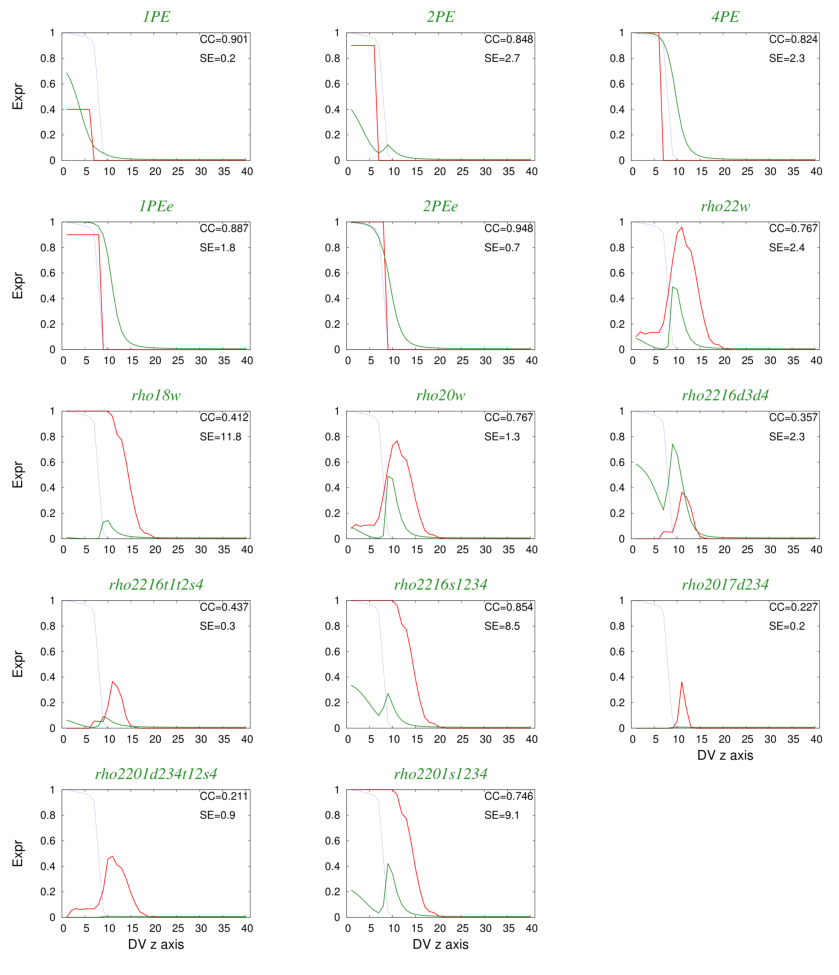
\includegraphics[width=1\textwidth]{DIb.pdf}\\
  \caption{the legend is in the upper right corner of the table, denoting the Observed profiles ( $E_t(z)$ ) as red, the model predictions as green along with the header above each figure denoting the CRM (gene target) in green, and the Dorsal morphogen profile  ( $E_{Dl}(z)$ ) as dotted blue curve.  The correlation coefficient between the observed pattern and the predicted pattern is denoted as CC for each gene (which is at most 'one'), and also the squared error between the observed pattern and predicted pattern is denoted as SE for each gene (where each gene had 40 positions, z, along the DV axis (i.e. SE is at most 40).  The Snail profile is uniform from positions 0 to 8, where it is 'on' (at a value of 'one') and Snail is off from positions 9 to 40 along the axis, and the Twist gradient (profile) was replicated as the Dorsal gradient. }\label{roughfit}
\end{figure}

\newpage

%\begin{table}
%\begin{tabular}{|c|c|c|c|c|c|}
%\hline 
%\omega_{Dl,Tw}(d_1)&	\omega_{Dl,Tw}(d_2)&	\omega_{Dl,Sn}(d_1)&	\omega_{Dl,Sn}(d_2)&	w_{Dl}&	w_{Sn} \\
%\hline 
%5&	64&	.1&	.7&	7&	39 \\
%\hline
%1.872&	37& 25& 12& .05 & 687\\
%\caption{The errors were estimated as the square root of the diagonal of $(J^TJ)^{-1}$, where the parameters estimated are in first row of the table, and their values in the second row of the talbe, and their standard deviation in the third row.  The $\chi^2=41$, where we had 1200 data points (each position along the z axis for each gene).  The Hessian, had a high condition number ($10^4$) where the largest eignevalue was 1.4, and the two smallest eigenvalues were .0002 and .001, suggesting that $\chi^2$ surface was close to flat along these dimensions of parameter space (i.e. the null space).}
%\end{tabular} 
%\end{table}
%

\subsection{Redesigning the parameters to be fit}
 
 The results above suggest poor nonlinear regression model design or insufficient data, where the free parameters to be fit from \ref{freeparams} were based off Segal's thermodynamic model, which was similarly used by Xin in GEMSTAT and Fukhouri et.al.\cite{pmid20087339}.  In general, the more parameters we add to the nonlinear regression model will either decrease the $\chi^2$ statistic (albeit, the reduced chi-squared that accounts for the degrees of freedom may increase) or it will maintain the $\chi^2$ statistic at a particular value (\textit{i.e.} the statistic becomes insensitive to additional parameters); but the $\chi^2$ will not increase.  This assumes one's fitting algorithm is allowed to 'find' the point along the newly added parameter's line in parameter space that improves the fit or at least does not spoil the smaller parameter set's fit.  Spoiling a previous fit with a newly added parameter can be avoided, for example, by simply setting the new parameter to a value where the model is insensitive (and hence $\chi^2$ will not be disturbed).  For model's with extensive dependencies between parameters this may not be possible.  However, by inspection, the parameters of our nonlinear model can all be set to values such that they have no contribution to the $\chi^2$.  For example, all the parameters in our nonlinear model, when set to numerically one, have the effect of not influencing the form of the model, in a sense, this is the parameter free form of the model.  I will call these values of the parameters the default values (\textit{i.e.} the default values have the odd property that it appears we are not fitting the parameters at all; and, in another sense, one could imagine fitting all the parameters and all the parameters being fit to the default values. ).  While setting the values to be zero have the effect of 'knocking out' all binding sites of a factor (in the case of $\alpha$) or 'knocking out' pairs of interacting binding sites (in the case of $\omega$)). 
 
   Fitting subsets of the parameters in Eq.\ref{freeparams} (such as a parameter subset without our novel pairwise potential $\omega$) leads to good fits, by eye, of the data, such as RMSE's of .05.  However, upon implementation of a Hessian matrix using a two point finite difference, we found that the Hessian matrix was not full rank for the parameter set even without the pairwise interactions $\omega$, our novel form of the potential.  Without pairwise interactions, one still has six free parameters to fit for the CRM's responses to Dorsal Twist and Snail morphogens.  Based on expert knowledge of the DV network, certain choices of two of the parameters were selected to fit the data, which occasionally lead to a Hessian with a condition number of about 100 (the condition number is a numerical technique to determine if a matrix is singular\footnote{In a computer, in a numerical representation, a matrix is rarely actually singular, it just has some eigenvalues that are much smaller than the largest eigenvalue of the matrix.  The number of eigenvalues of Hessian is the number of parameters to be fit, and if some of these eigenvalues are close to zero, this suggest a zero determinant Hessian.}), while many of the choices of parameters lead to Hessians with condition numbers on the order of $10^4$.  Furthermore, the Hessian should be positive definite for a unique solution, while we found the eigenvalues were frequently mixed in sign (indicating saddle points) - of course the gradient (the derivative of the $\chi^2$ with respect to each parameter, a different object from the Jacobian) was zero (on the order of $10^-{10}$ for each component) at all of our estimates of the minima of the $\chi^2$ surface\footnote{These results lead to the implementation of the Levenberg Marquardt that has a number of GSL built in functions to help diagnose pathological nonlinear models (unlike the gradient descent and simplex implementations).  If Levenberg Marquardt revealed the same types of errors in our parameter estimates then we could be more confident that there was not an error in our implementation of the Hessian.  (i.e. a zero determinant Hessian, means our parameter error bars are infinite in extent - unless one decides to use a different method to estimate their error bars).}.
 
%  For example, the finite difference Hessian was found to be unstable for step sizes smaller than $10^{-^$ presumably due to 'catastrophic cancellation' (subtraction of two numbers with different number of significant figures).

In order to better estimate the errors of the parameters for our model we aimed to obtain a full column rank Hessian (regardless of whether the Hessian was positive definite).  We analysed the analytic derivative of our nonlinear model with respect to each parameter $\beta_i$, and checked if other parameters occur in the result (indicating dependencies between parameters).  If possible, parameters that do depend on one another were grouped to form just one parameter\cite{beck}.  Furthermore, certain regions of the Data space (such as certain positions in the embryo (like the dorsal ectoderm, where none of our genes are active) may be very insensitive to our parameters (causing small values of the Jacobian for these data points, however this does not appear to affect the Hessian of the $\chi^2$, since the analytic Hessian, $\mathcal H$ of the $\chi^2$ is exactly equal to $J^TJ+G$, where G is a matrix of second derivatives over the model\footnote{The analytic Hesssian in exact form is  $\mathcal H=\frac{\partial^2{\chi^2}}{\partial{\mathbf{\beta}}\partial{\mathbf{\beta}}} = J^TJ + \frac{\partial^2{f}}{\partial{\mathbf{\beta}}\partial{\mathbf{\beta}}} = J^TJ +G$, where G is matrix with second derivative elements of the nonlinear model f (the fractional occupancy of the BTA) over the model parameters (for example, see equation A.4c page 482 of Beck\cite{beck}).  In the case that G's Frobenius norm is nearly zero (the elements of G are nearly zero), then we have $\mathcal H=J^TJ$, which is why with certain data sets and experiments, it is possible to estimate the covariance matrix of parameters based on Jacobian alone.  $J^TJ$ for the case of one free parameter is just a dot product (i.e. the Jacobian is just a vector of size n x 1, where n is the number of data points), which will be insensitive to data points that were uninformative for parameter estimation (they're just adding a term zero to the dot product).  Hence, it seems reasonable that uninformative data (data where the model is insensitive, such as Dorsal ectoderm regions of the embryo, where none of our CRMs are active) will not cause harm to model fitting.}.  

%}.  Hence inverting the Hessian in the case that G is small (which it is for cases like the dorsal ectoderm data points, will require inverting $J^TJ$, but if there are many terms that are zero in the Jacobian (zero due to selecting data points where the model is insensitive to variations of the parameter), then $J^TJ$ will also be noninvertible (zero determinant).
\subsection{ Analytic Jacobian }
A simple function is $f(z)=1/(1+\exp(-\beta z))$, where $\beta$ is a constant, where the domain and range of $z$ and $f$ are: $z \in [-\inf,\inf] \ \ f(z) \in [0,1]$.  Now if we imagine that $\beta$ was a free parameter, then we could ask how sensitive this function is to variations of $\beta$ as a function of particular positions along the domain of z.  Hence the derivative is:
\begin{equation}
 \frac{\partial{f(\beta,z)}}{\partial{\beta}}= \frac{\beta \exp{(-\beta z)}}{(1 + \exp{(-\beta z)})} \approx  \beta f(z,\beta) (1-f(z,\beta))
 \end{equation}
 The above equation, in a sense, is an analytic representation of the Jacobian matrix elements for the nonlinear model (e.g. BTA occupancy) as a function of data (all possible data, which is represented by the domain of z).  
 
 We do not need to analyze our more complicated BTA occupancy function to understand the behavior of the Jacobian matrix elements, rather we can simply use the above equation as a phenomenological parametrization of our model of CRM response to morphogen gradients (which are encoded in the spatial position $z$).  For example, imagine one wished to analyze phenomenologically the response of \textit{rhomboid} expression pattern just in the positions of the embryo of the neuroectoderm and the dorsal ectoderm (in our binning of the DV axis this would be equivalent to the z interval of [9,40], where the interval [1,8] contains the mesoderm, which we are uninterested in for the moment).  We can model the $rhomboid$ expression as a function of DV axis using the above equation, where we set $\beta$ to be negative since we must reflect the function about the 'switch' point where the gene is turned 'on (the point in space where $rho$ turns 'on' is at the neuroectoderm-ectoderm border).  \footnote{If we modeled the 'switch' point where the gene is turned 'off' (the point in space where $rho$ turns 'off' is at the mesoderm-neurectoderm border) we would not have to reflect our graph about the switch.}  We must also offset the position where the logistic function reaches $1/2$ max (which in the above equation is position $z=0$).  Hence we mush add a constant to the argument of the exponential $$f(z)=1/(1+\exp(\beta z -\beta_0 ))$$, where $beta_0 $ will define the $1/2$ max of the logistic function when $z\beta=\beta_0$.
 
The analytic Jacobian for these two parameters (as a function of data z):
\begin{equation}
\frac{\partial{ f}}{\partial{ \beta}} = \frac{-z\exp{(\beta z-\beta_0)}}{(1+\exp{(\beta z-\beta_0)})^2}=-z f(1-f)
\end{equation} \footnote{The logistic function when evaluated at a particular point $z'$ can be thought of as a Bernoulli Distribution, hence, the last expression is the variance of the Bernoulli distribution, where the function $f(x')$ at each point $x'$ happens to be the 'parameter' that describes a Bernoulli distribution (normally this parameter is denoted as 'p' for probability, where the mean of Bernoulli random variable is also p, and the variance of a Bernoulli random variable is p(1-p).  This is effectively how the BTA occupancy is described along the DV axis where $x'$ now denotes the position along the DV axis, and $\beta$ is a free parameter.}
\begin{equation}
\frac{\partial{f}}{\partial{ \beta_0}} = \frac{\exp{(\beta z - \beta_0)}}{(1+\exp{(\beta z-\beta_0)})^2}= f(1-f)
\end{equation}
\footnote{Do these two two equations span parameter space?  Recall previously we analyzed $\exp{(\beta_1 +\beta_2) z}$ for its behavior in the context of nonlinear regression.  Similarly for the logistic nonlinear model we would like to analyze $1/(\exp{(\beta_0 +\beta z)}$.  For example, and if one knows with certainty two independent data points $(y_1, x_1), (y_2,x_2)$, then we can transform to a simple linear model for the above equation, where one arrives at the following system of equations $\begin{pmatrix}  1&x_1\\ 1 & x_2\\ \end{pmatrix} \begin{pmatrix} \beta_0\\ \beta \\ \end{pmatrix} = \begin{pmatrix} \ln{\frac{y_1}{1-y_1}}\\ \ln{\frac{y_2}{1-y_2}} \\ \end{pmatrix} $.  Does this span the $\beta,\beta_0$ plane (the parameter vector space)?  The determinant of the design matrix is $x_2-x_1$, which suggest as long as the experimental design was such that the data points $x_1$ and $x_2$ are not too close together we could actually 'fit' $\beta_0$ and $\beta$.  However, one must be careful here, since data collected in regions of very large or very small $x_1$ and $x_2$, will cause the original response $y$ to become close 'one' or 'zero' causing the logarithm's value to be very large, possibly causing numerical issues.  This can be seen by symbolically solving for the eigenvalues of the design matrix, where we must solve for the roots of $(1-\lambda)(x_2-\lambda)-x_1=\det(X-\lambda I)=0$), where X is design matrix, and $\lambda$ is the eigenvalues of the design matrix.  This yields the quadratic $\lambda^2 +x_2\lambda+x_2-x_1$.  If $\lambda$ is zero (which means we would have a singular design matrix) we see that indeed $x_2=x_1$, which makes sense, we can't expect repeated measurements of the same position in space to tell us anything about the global behavior of the sigmoid (as defined by the $\beta$ parameters).  Solving the for the roots of the polynomial using the quadratic formula we have:
\begin{equation}
\lambda=-\frac{x_2 \pm \sqrt{x_2^2-4x_1}}{2},
\end{equation}
here we know constraints on the data due to the embryo size, where the DV portion of the embryo constrains $[x_1,x_2]$ to reside in the interval $[0,40]$, since there are only 40 cells along that axis.  Given the constraint on embryo size it seems we can at least say $\sqrt{4x_1}<x_2$.}

Now we can see some simple relations. First of all $J^TJ$ =0 if one only collected data in the dorsal ectoderm region of the embryo (where the logistic is nearly '1', meaning we can not invert that matrix (so J is not full column rank).  Similarly, if one just has Boolean data for the expression pattern of $rho$ along the z axis, say 00000001111111100000000=$\bm{E}_rho$, the only possible point where J is nonzero is at the borders  where the gene switches from off to on or vice versa.  Now imagine for an NEE gene that we have an expression pattern over space like 0000000101010100000000 where the switching behavior (10101010) is in the neurectoderm region of the embryo, while the other two regions are the mesoderm and ectoderm.  Using a mathematical metaphor, it is as if one has $J^TJ_{meso} + J^TJ_{neuro} + J^TJ_{ecto} =J^TJ = J^TJ_{neuro}$, since the regions in data space of $meso, \ ecto$ are insensitive to parameter variations, hence these regions in data space (the row space of $J$), act as labels to the null space of $J^TJ$ that is a subspace of parameter space (the column space of $J$). 



%, though, since the actual matrix expansion of the above form is in the form of a set of rank one eigenvectors of the matrix $J^TJ$ (spectral theorem)\footnote{If one has an underdetermined system, then $J^TJ$ will be singular, and hence will have a set of degenerate eignenvalues of zero; which correspond to a set of eigenvectors, these eigenvectors span the null space of the symmetrized matrix $J^TJ$,  I can \emph{choose} them to be orthogonal (always possible for symmetric matrices).  These eigenvectors are in the parameters vector space, while the labels $meso$ and $ecto$ are in the data vector space.  I suspect that it is these regions in the embryo's axis of measurement that I suspect are insensitive to parameter variations (and hence in some sense, could be used as labels for the matrix $J^TJ$).}.

\subsection*{Analysis of binding energy effects on occupancy}
For one binding site, we can compute the average occupancy, it is just the probability of the bound configuration $P(c=1)$ where $c=1$ is the configuration vector in the bound state (c takes on only two values 1 or 0 ).
\begin{equation}
\frac{\partial{P(c)}}{\partial{E(S)}} =  P(c)(1-P(c))
\end{equation}
This function's maximum is .25, which occurs at $P(c)=.5$.  Hence the greatest effect of energy on the occupancy of one site is at half max occupancy. 
% Furthermore, we can estimate the binding process as poison for small $P(c)$, in which case $P(c)(1-P(c))\approx P(c)$.  Hence, for low occupancy, the error in the occupancy is about $\sigma_{P(c)}=P(c)$, therefore $\partial{E(S)} = \sigma_{E(S)} = \frac{\sigma_{P(C)}}{P(C)}=1$. 
Assuming the differentials are standard deviations we have:
\begin{equation}
 \sigma_{P(C)}=|P(c)(1-P(c))| \sigma_{E(S)}.
  \end{equation}  
% Solving for $\sigma_{E(S)$ we have:
% \begin{equation}
%  \sigma_{E(S)= \frac{\sigma_{P(c)}}{|P(c)(1-P(c))|},
% \end{equation}
% which for small $P(c)$ the we have  $\sigma_{E(S)= \frac{1}{\sqrt{P(c)}}$.
%\textit{What is approximately the minimum energy that can influence the configuration vector?}     

% If one places constraints on the range that the free parameters are allowed to fit, we can put a bound on the maximum energy of a binding site that can cause a differential effect on our model of a specified size.  For example, we may be uninterested in effect sizes as small as $|df|=|.01|$, which means the fractional occupancy of the BTA has changed by .01.  For a module of just one site, what is the highest possible energy that can cause an effect size of this magnitude?
%
%We simply need to calculate $df/dE$ analytically, and then solve for dE, setting df equal to .01.  It is helpful to analyze the effect of  energy sizes on the occupancy of morphogens (i.e.$ d<n>/dE$).  Here we will just analyze one binding site (therefore the expected occupancy of the binding site is equal to the probability of the site being bound $<n>=P(c_b)$, where $c_b$ is the bound configuration.
%
%\begin{equation}
%\frac{\partial{n}}{\partial{E(S)}} = E(S) <n>(1-<n>)
%\end{equation}
%  
%Hence the change in occupancy when there is a mutation in the site that increase the energy by $E(S)$ will have the effect $\partial{E(S)}$ and the :
%  \begin{equation}
%\partial{<n>}= (\partial{E})^2 <n>(1-<n>)=
%\end{equation}
%The variance of a boolean variable $<n>(1-<n>)$ is maximal at $<n>=1/2$, hence at half max occupancy the occupancy is most sensitive to perturbations of the energy. We would like to know what is the energy required to have an effect as small as $|d<n>|=|.01|$, which means the fractional occupancy of the morphogen has changed by .01.  In general we have:
%\begin{equation}
%\partial{E}=\sqrt{\frac{|d<n>|}{<n>(1-<n>)}}.
%\end{equation}
%Hence, for the case of interest we need to plot the function:
%\begin{equation}\label{difE}
%\partial{E}=\sqrt{ \frac{.01}{<n>(1-<n>)} },
%\end{equation}
%which is shown in figure \ref{diffE}:
%\begin{figure}
%  \includegraphics[width=1\textwidth]{diffE_3ener.eps}\\
%  \caption{Three different binding energy levels are analyzed, 1 (blue), 5 (red), and 10 (green).  At each energy level $\partial E=dE$ is calcualted from Equaton \ref{difE} to determine the amount of energy required to obtain a 0.1 increase in the occupancy of binding sites at that energy level. }\label{diffE}
%\end{figure}

%An energy of 9 is a Boltzmann factor of $\exp{(-9)}=.0001$, and energy of 4 is a factor of $\exp{(-4)}=.02$.  In our model the weight of a CRM with a single site in the bound configuration ($c_b$), has the following Boltzmann factor, $W(c_b)=q_i=K(S)[tf(i)]=K_0\exp{-E(S)}\frac{E_{tf}(k)}{E_{tf}(max)} = \exp{-E(S)}E_{tf}(k) \alpha_{tf}$.  We only use two significant figures for the expression data, hence the minimum value of $E_{tf}$ (excluding zero) is 0.01.  $\alpha_{tf}$ is the a free parameter to be fit bounded between $[1,100]$, hence the minimum value of $\alpha$ is 1.  Hence, the configuration weight with the smallest possible parameter and concentration case for an energy of 9 has a configuration weight for the bound case $W(c_b)= .01*.02=.0002$.  For modules with two identical binding sites of this energy, when all the sites are bound we would have a configuration weight of $(.0002)^2$ .  While the configuration weight with largest possible parameter ($\alpha_{max}=100$) and concentration ($E_{tf}(max)=1$) results in $W(c_b)=\alpha_{max}*E_{tf}(max)\exp{(-E=9)}= 100*1*.02=2$.  For modules with two identical binding sites of this energy, when all the sites are bound, then we would have a configuration weight of $(2)^2$.  Hence, in the case that $\alpha=100$ and $E_{tf}=1$ for a binding energy of 4, we see a binding site with energy 4 is actually at half max occupancy $<n>=1/2$; and that if the CRM had two binding sites of this energy, then the module reaches one full unit of occupancy of the transcription factor $<n>=1$ under peak concentrations and peak values of $\alpha$ (which is like a factor that has a large $K_0$).  We won't go through in detail the case of 9, but we do want to see that under peak conditions we would have $W(c,b)=\alpha_{max}*E_{tf}(max)\exp{(-E=9)}=100*1*.0001=.01$.  This $1\%$ the size of the weight for the unbound case $W(c_u)=1$, this means $<n> \approx .01$.  
%
%The effect of the occupancy of the morphogen on the BTA is based on our model: ($f_{BTA} = logit(w_0 + \sum_{tf } \ w_{tf} < n_{tf} > )$, where we have written our model in terms of the famous logit function which is the 'canonical link' to the odds of the $f_{BTA}$.  Hence, the log odds is:
%\begin{equation}
%   \log{\frac{f}{1-f}}= w_0 + \sum_{tf } \ w_{tf} < n_{tf} > 
%   \end{equation}   
%now if we take the log \emph{odds ratio}, where we assume $df= f_f - f_i=0.01$ is due to an increment in the energy $dE(S)$ (a yet to be determined increment in energy, which hereafter will be called $\Delta \epsilon$), where $f_i$ is the initial occupancy of the BTA, and $f_f$ is the final occupancy of the BTA, we then have:
%
%\begin{equation}
% \log{\frac{f_i}{1-f_i} \frac{1-f_f}{f_f}}=  w_0 - \sum_{tf} \ w_{tf} < n_{tf} >_i  - (w_0 - \sum_{tf } \ w_{tf} < n_{tf} >_f ).
%\end{equation}
%Now we now the log odds is zero when the occupancy of the BTA is half max.  Hence we have:
%\begin{equation}
% \log{\frac{1-f_f}{f_f}}=\log{\frac{.4}{.6}}=  \sum_{tf } \ w_{tf} < n_{tf} >_f   - \sum_{tf } \ w_{tf} < n_{tf} >_i 
%\end{equation}
%Now, assuming the CRM has just one binding site we for a transcription factor $tf$ we have:
%\begin{equation}
% \log{\frac{1-f_f}{f_f}}=\log{\frac{.4}{.6}}= \ w_{tf}( < n_{tf} >_f  -  < n_{tf} >_i ),
%\end{equation}
%where we can treat the energy decrement $\Delta \epsilon$ from the initial binding site to the new binding site as a perturbation factor in the canonical partition function, q, we then have:
%\begin{equation}
%  < n_{tf} >_f  -  < n_{tf} >_i = \frac{1}{1+q\exp{(-\Delta \epsilon)}} - \frac{1}{1+q}
%\end{equation}
%creating a common denominator and using the symbol $y=\exp{(-\Delta \epsilon)}$ we have:
%\begin{eqnarray*}
%\frac{1}{1+qy} - \frac{1}{1+q} &=& \frac{ q(1+y)}{(1+qy)(1+q)}\\
%&=& x,
%\end{eqnarray*}
%
%here x is the value of the log odds ratio, which we know.  Now after some algebra we arrive at:
%\begin{equation}
%\Delta \epsilon = -\ln{ \frac{  x (1+q)/q -1  }{ x(1+q) + 1}  }
%\end{equation}
%The value of the log odds ratio was 0.4, hence, an increment of $20\%$ of the occupancy of the BTA, in this case, is from a change in the binding site energy (due to a new binding site sequence) of:
% \begin{eqnarray*}
%\Delta \epsilon &=& -\ln{ \frac{ .4 (1+\alpha_{max}E_{tf}(max)\exp{-E(S)})/(\alpha_{max}E_{tf}(max)\exp{-E(S)}) -1  }{ .4(1+\alpha_{max}E_{tf}(max)\exp{-E(S)}) + 1}  }\\
%&=&-\ln{ \frac{ .4 (1+100\exp{-E(S)})/(100\exp{-E(S)}) -1  }{ .4(1+100\exp{-E(S)}) + 1}  }\\
%&=& 9.2
%\end{eqnarray*}
%Here we have assumed the initial binding site has $E(S)=0$, the ground state, furthermore we assumed that $w_{Dl,BTA}$ was 1.   

\subsection*{Balanced Data sets of mesoderm and neurectoder enhancers, Experiment 2}
The parameters of the thermodynamic model are all contingent on the free parameters that correspond to Snail (such as it $\alpha$ for its protein-DNA interaction, and its quenching strength, and its $w_{SN}$ for Snail's strength of repressing BTA binding).  Hence, to disentangle the cooperativity of Twist and Dorsal (if it exist) from the other free parameters, an experiment was conducted with no Snail protein (no Snail in the network).  Hence, the MPA simply annotates for Twist and Dorsal (where again the MPA was not 'fit' rather default parameters were set for annotation).  All NEE modules are known to be repressed by Snail in the mesoderm.  However, the cooperativity of Dorsal and Twist is known to be important when there are limiting concentrations of Dorsal in the neuroectoderm (where Snail protein does not exist).  Furthermore, the modules that are not NEE's (such as mesoderm targets of Dorsal), are know to have no Snail binding sites in their module (at least this will be hypothesis).  Here we used four CRMs to fit two parameter, the Dorsal binding strength and Dorsal-Twist cooperativity.  We found a $\chi^2=8.9$ for 80 data points\footnote{The goodness of fit can be tested here, with 78 degrees of freedom, we can assume our fit is a deviate from the $\chi^2$ distribution.  If the value of our squared error is a reasonable deviate from the $\chi^2$ distribution then we can accept the fit.  I computed the p-value as nearly one, suggesting the fit is good (the cdf of our the $\chi^2$ distribution to the value we found was $10^{-28}$. }.    We removed the constraint on the parameter ranges, and set $w_0= 5$,  $w_{Dl}=-5$, $w_{Tw}=0$.  We set $w_{Dl}=5$ because we wanted one unit of Dorsal occupancy to correspond to half max BTA occupancy (which means the target gene is at half max).  We set $\alpha_{Tw}=1$, the default value.  We found $\alpha_{Dl}=0.3 +/- 0.03$, and $\omega_{Dl,Tw}=3980 +/- 982$, where the standard deviations were estimated from the square root of the corresponding parameter's diagonal element of $(J^TJ)^{-1}$.  The   

These results are as expected from the modules shown.  For example, the construct $6xdl$ was a Szymanski construct that was shown that even with 6 Dorsal binding sites, the CRM does not respond to Dorsal in the neuroectoderm (see profile in Figure).  Hence, if these were zero energy Dorsal sites, then we know for what was defined as the minimum value of $\alpha_{min}=1$ that Dorsal occupancy would reach half max at the position z and a concentration $E_{Dl}(z)$, hence we have: $E_{Dl}(z)/(1+E_{Dl}(z))=<n_{Dl}>= 1/2$, hence $E_{Dl}(z)= 1$.  However, the CRM $6xdl$ had 6 Dorsal binding sites, hence one unit of occupancy could be reach at 1/6 this concentration (since the sites are all independent, by assumption).

Another construct that was used was the double knock out of Twist sites by Ip, which reported catastrophic loss of expression in the neuroectoderm, the construct labelled $rho2216t1t2s4a$.  Hence the Ip construct along with the $6xdlPLZ$ acted as a control group.  The treatment group (in a sense) were two constructs that are known to have Twist sites the $rho$ CRM (from $mel$ specie), and the $vn$ CRM (from $vir$ specie).
 
The Snail protein was not used in this model, , and the Twist gradient (profile) was replicated as the Dorsal gradient.  The $6xtwPLZ$ was also left in the training set, but this has negligible effect (due to model assumptions (i.e. default parameter values of Twist), and the reported expression profile by Szymanski for a this construct was roughly zero (i.e. Twist binding sites alone are not sufficient)).
\begin{figure}
  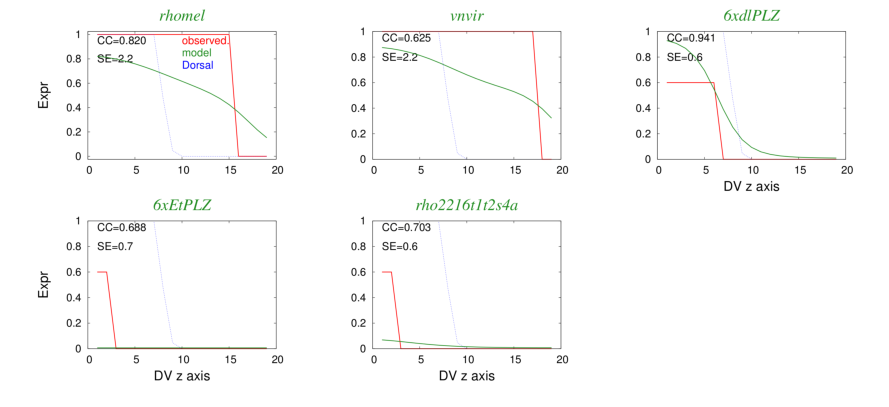
\includegraphics[width=1\textwidth]{DInosnail.pdf}\\
  \caption{the legend is in the upper right corner of the table, denoting the Observed profiles ( $E_t(z)$ ) as red, the model predictions as green along with the header above each figure denoting the CRM (gene target) in green, and the Dorsal morphogen profile  ( $E_{Dl}(z)$ ) as dotted blue curve.  The correlation coefficient between the observed pattern and the predicted pattern is denoted as CC for each gene (which is at most 'one'), and also the squared error between the observed pattern and predicted pattern is denoted as SE for each gene.  Each gene had 20 positions, z, along the DV axis, which as always (in DV literature), is plotted such that ventral is at the zero position.  }\label{roughfit}
\end{figure}


\begin{figure}
  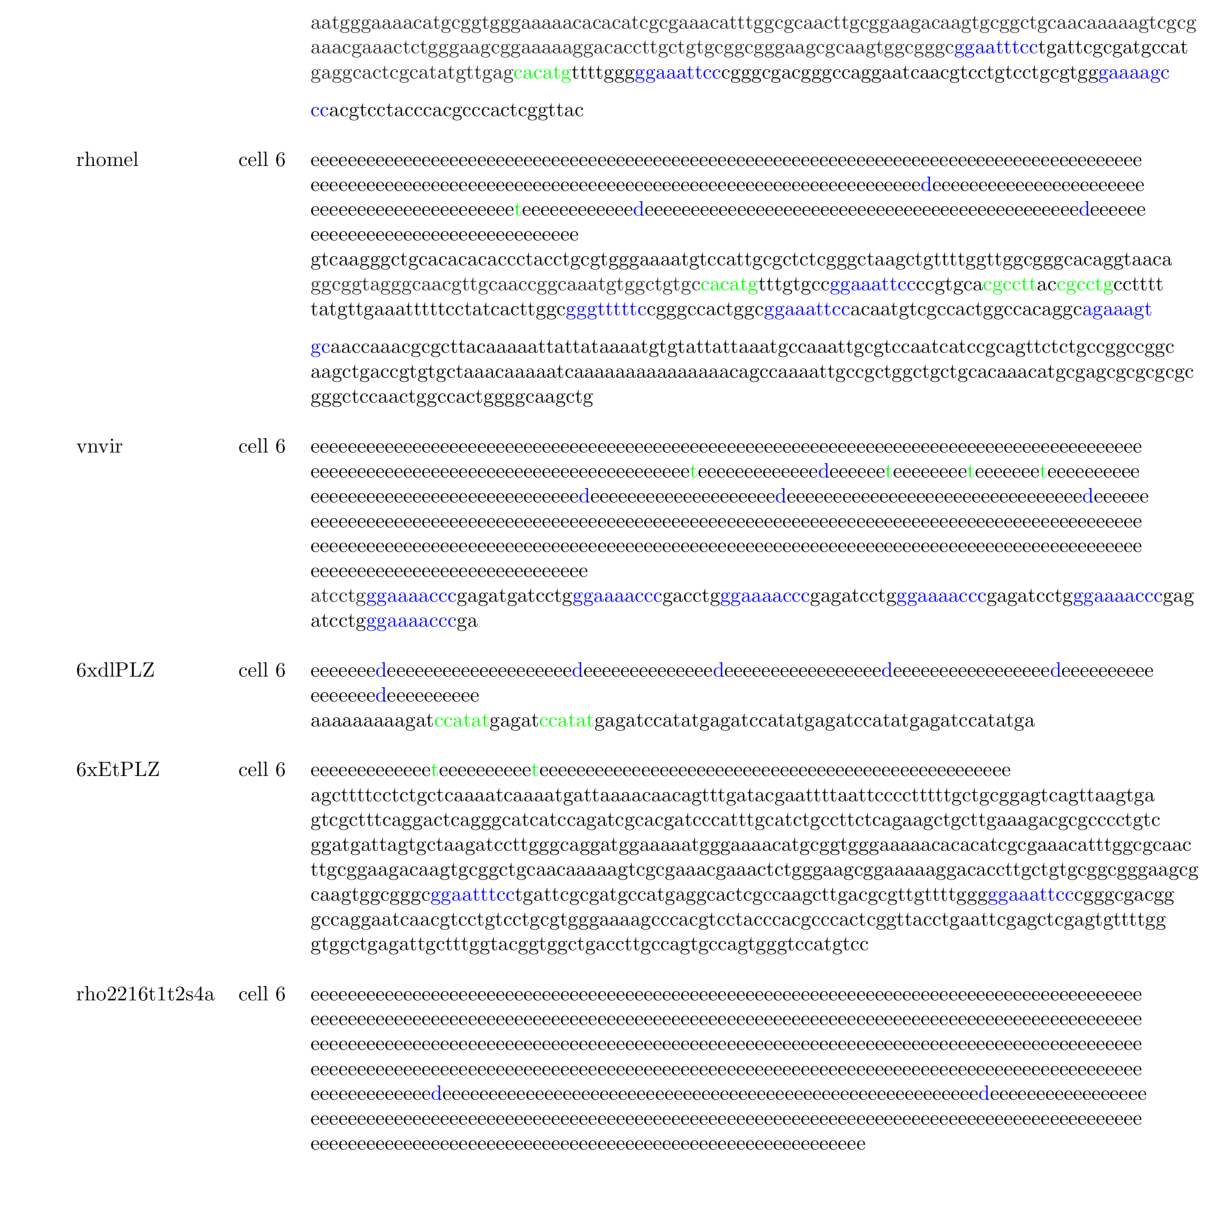
\includegraphics[width=1\textwidth]{annNosnail.pdf}\\
  \caption{The CRMs and predicting binding sites from MPA for default parameters on all proteins.  Dorsal annotated blue, Twist green. The column d+ denotes added noise to Dorsal concentration profile (which was zero in this case, hence d+ should not be there).  A bug in the printing code caused one of the $vnvir$ sites to not appear in the CRM sequence highlighting. }\label{roughfit}
\end{figure}
%Hence we could simply not model the mesoderm, and contrast NEE's that have variation in their patterns from the dorsal ectoderm to the ventral-most region of the Neuroectodem (the mesoder-neuroectoderm border).




\subsection{ Robustness analysis, Experiment 3 }
We increased the Dorsal expression by .15 in each position along the DV axis to see if the annotated binding sites were the same when using the annotation model MPA.  The data set was four NEE modules $rhomel, rhovir, vnmel, vnvir$.


The Twist gene's free parameters were all set to 'one' for $\alpha$, and $\omega_{Tw,Dl}$ was set to 'one' for all bins except $B=[0,20]bp$, and $w_{Tw}$ parameter was set to zero.  Furthermore, the Twist's morphogen concentration gradient $\bm{E_{Tw}}$ was set equal to Dorsal's gradient to assure their differential gradients were not influencing the result.  Snail's quenching was set for $w_{Sn,Dl}$ for only one bin $B=[0,50]bp$ (quenching means $\omega$ is in the range [0,1], while cooperativity means $\omega$ is in the range [1,100].  Hence, we only allowed the Dorsal and Snail parameters to be tuned by the fitting routine.
 
The results of annotation with the wild-type Dorsal expression (no perturbation of the profile) are in figure\ref{annb}.  The results of the perturbed Drosal profile are in figure \ref{annc}.  The annotations are the identical.  This possibly is an artifact of the way the Dorsal profile was perturbed (by simply adding .15 to each cell).  Due to the sigmodal nature of the Dorsal profile this has little effect.  A better designed experiment would shift the half max of the Dorsal profile by a fixed number of positions along the z axis.


%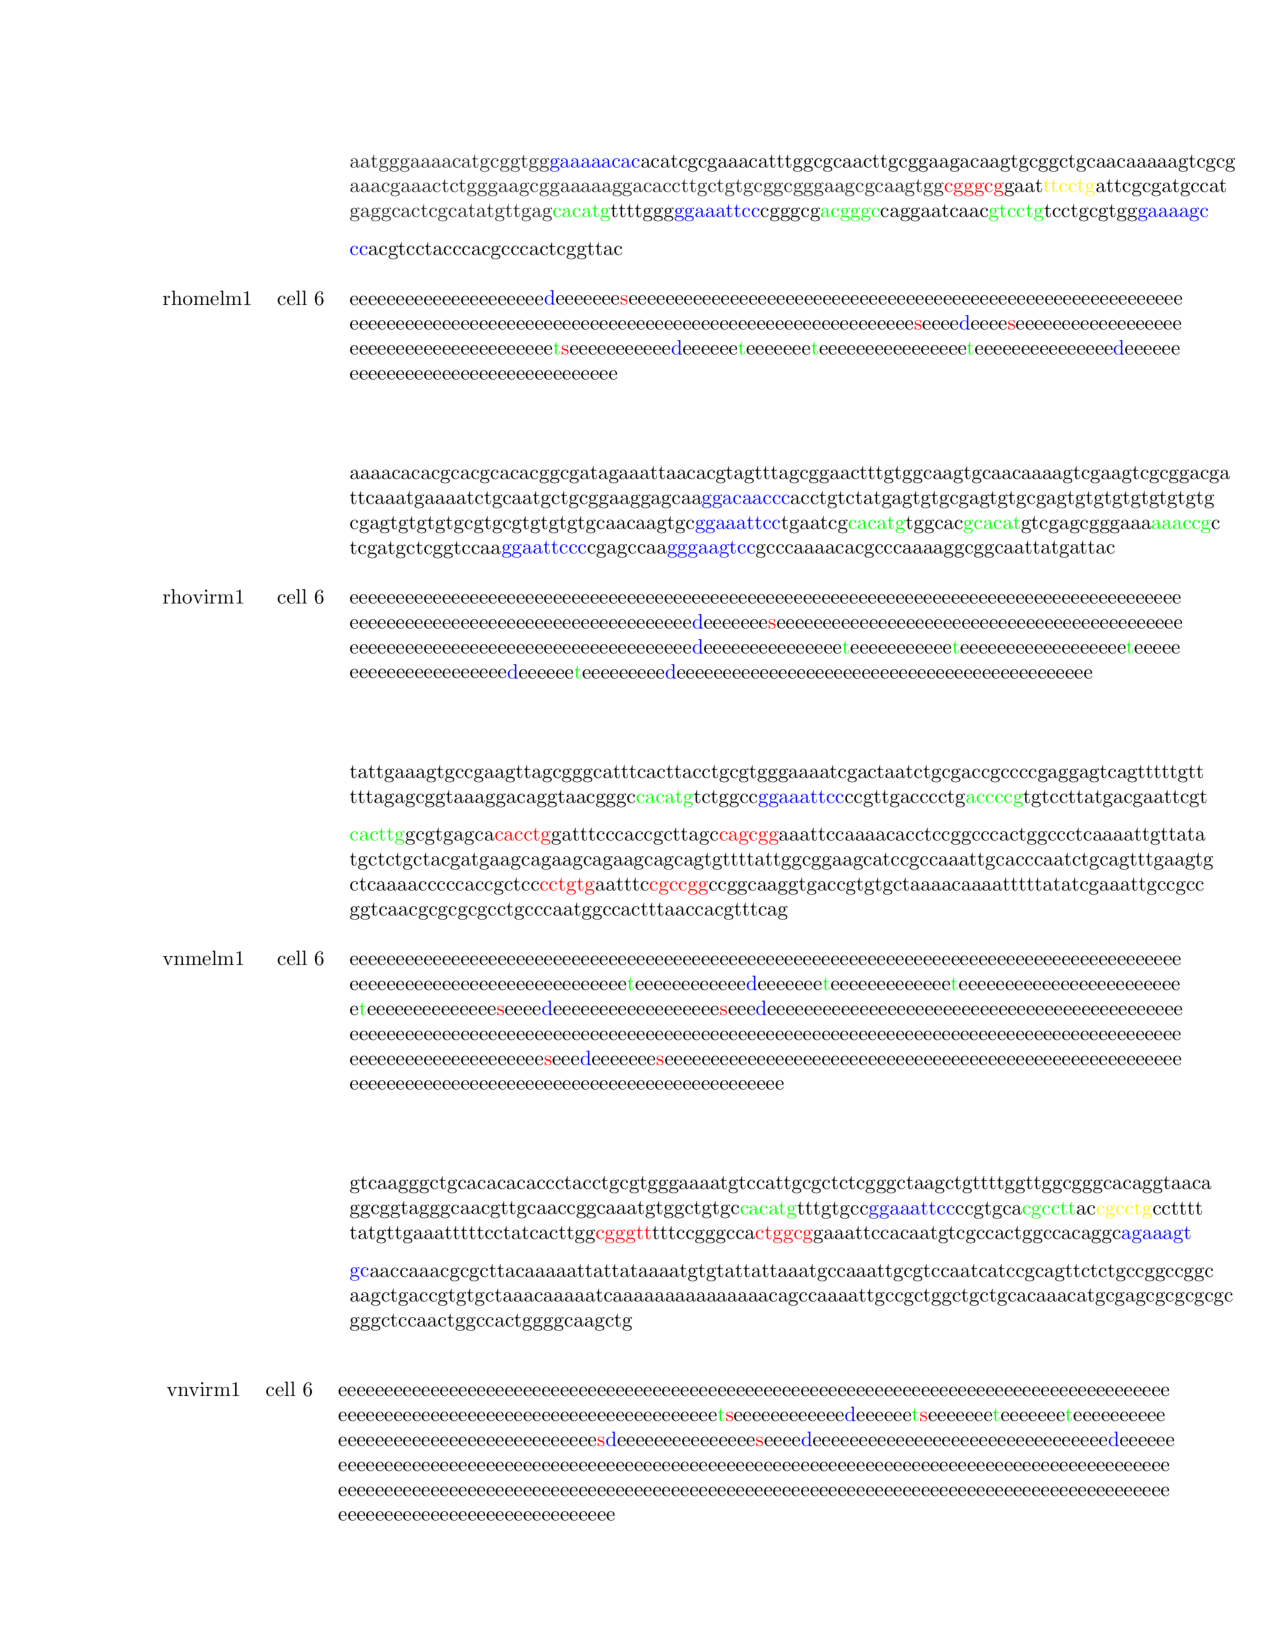
\includepdf[pages=-]{annb.pdf}
\begin{figure}
  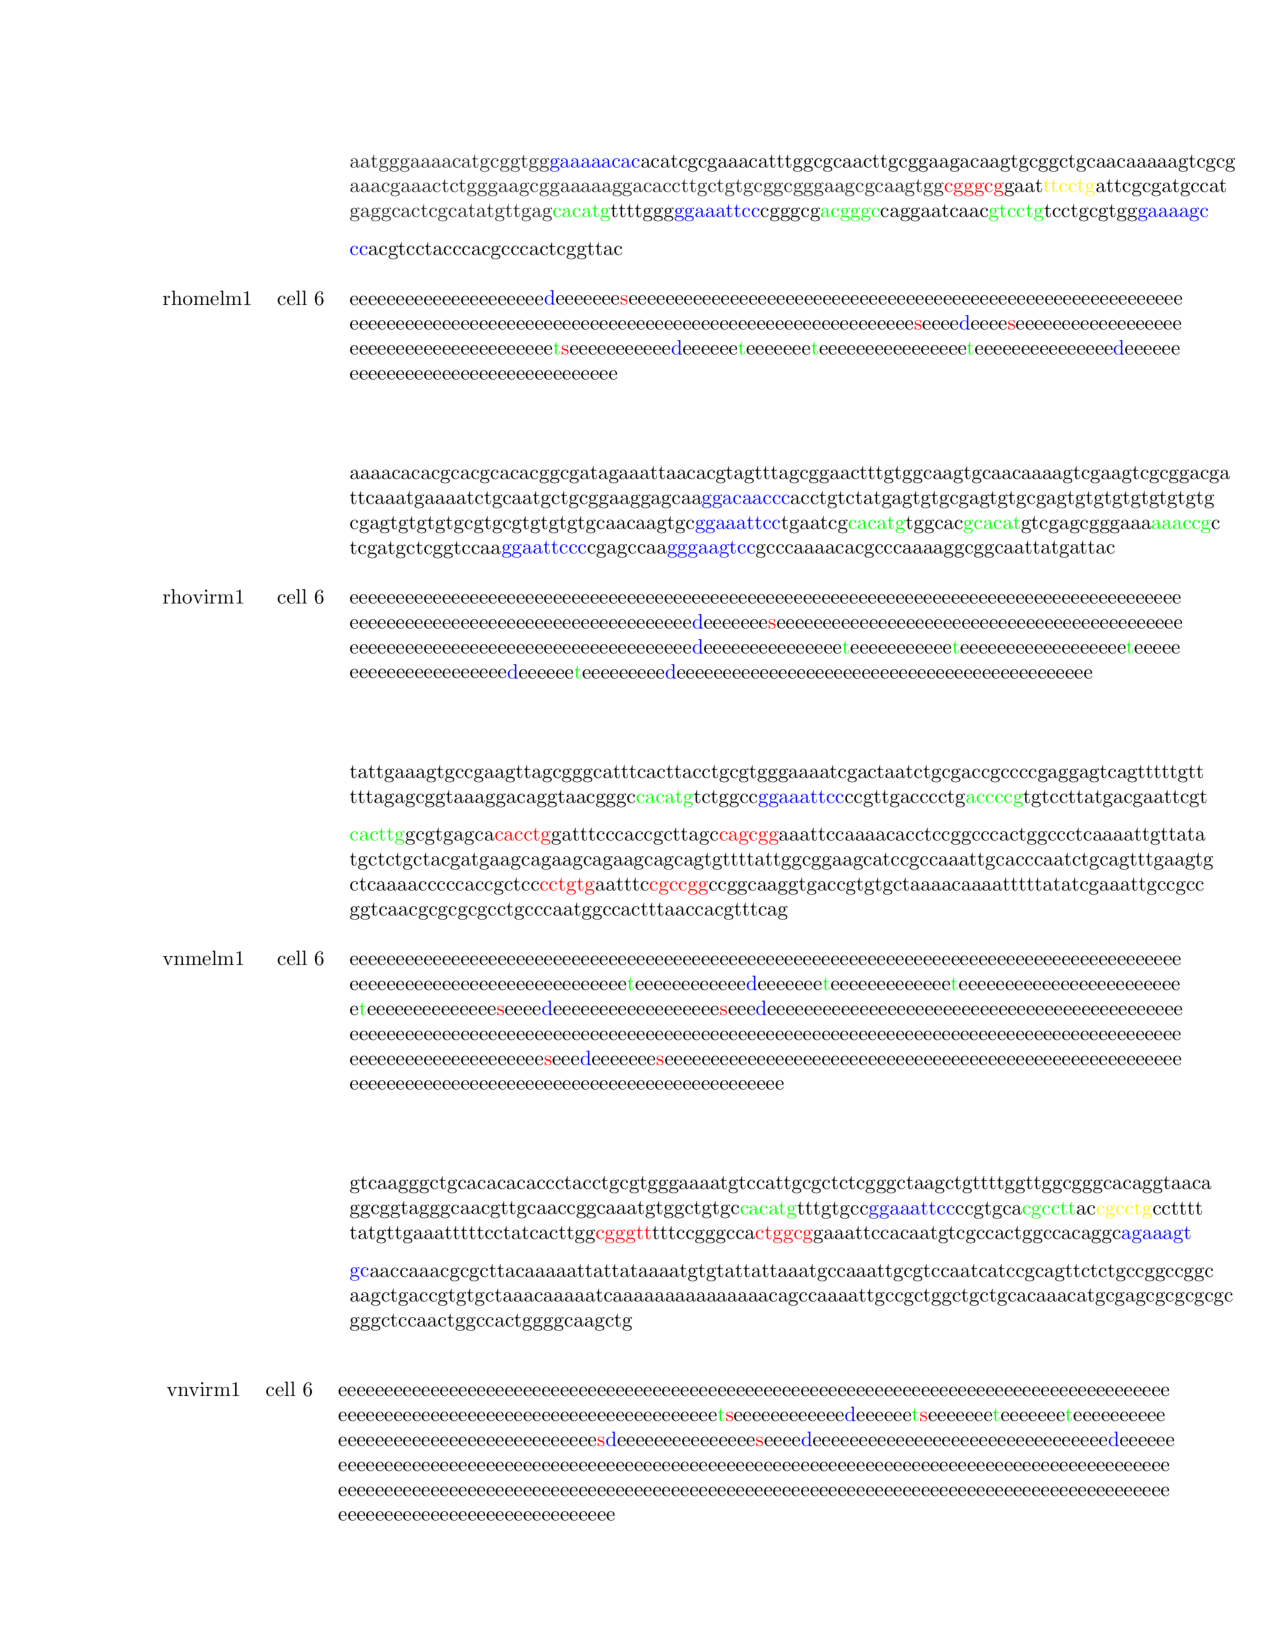
\includegraphics[height=1\textwidth]{annb}\\
  \caption{Here the target gene is denoted in the left column, and the cell along the DV axis is denoted in the second column.  Twist site's are annotated green, Dorsal blue, Snail red, and brown denotes overlaps.  The sites annotated at the mesoderm bottom border were used to annotate the sequence.  For example, the first gene is $\emph{rhomel}$, for \textit{rhomboid} in the species $melanogaster$. }\label{annb}
\end{figure}
%The expression profiles for the above CRMs are shown in following graphs, where the annotated binding sites were based on the gene's corresponding annotation from the mesoderm 'm1' condition.  In addition to showing the correlation coefficient (CC) between model and observations, and the squared error between model and observations (SE), we show the absolute error (AE), which is the absolute value of the difference between the model predictions and the observed pattern. 

%\includepdf[pages=-]{DI.pdf}

%\begin{figure}
%  \includegraphics[height=.8\textwidth]{DI.pdf}\\
%  \caption{the legend is in the upper right corner of the table, denoting the Observed profiles ( $E_t(z)$ ) as red, the model predictions as green along with the header above each figure denoting the CRM (gene target) in green, and the Dorsal morphogen profile  ( $E_{Dl}(z)$ ) as dotted blue curve.  The correlation coefficient between the observed pattern and the predicted pattern is denoted as CC for each gene, and also the squared error between the observed pattern and predicted pattern is denoted as SE for each gene (where each gene had 40 positions, z, along the DV axis.  The Snail profile is uniform from positions 0 to 8, where it is 'on' (at a value of 'one') and Snail is off from positions 9 to 20 along the axis, and the Twist gradient (profile) was replicated as the Dorsal gradient. }\label{roughfit2}
%\end{figure}
\begin{figure}
  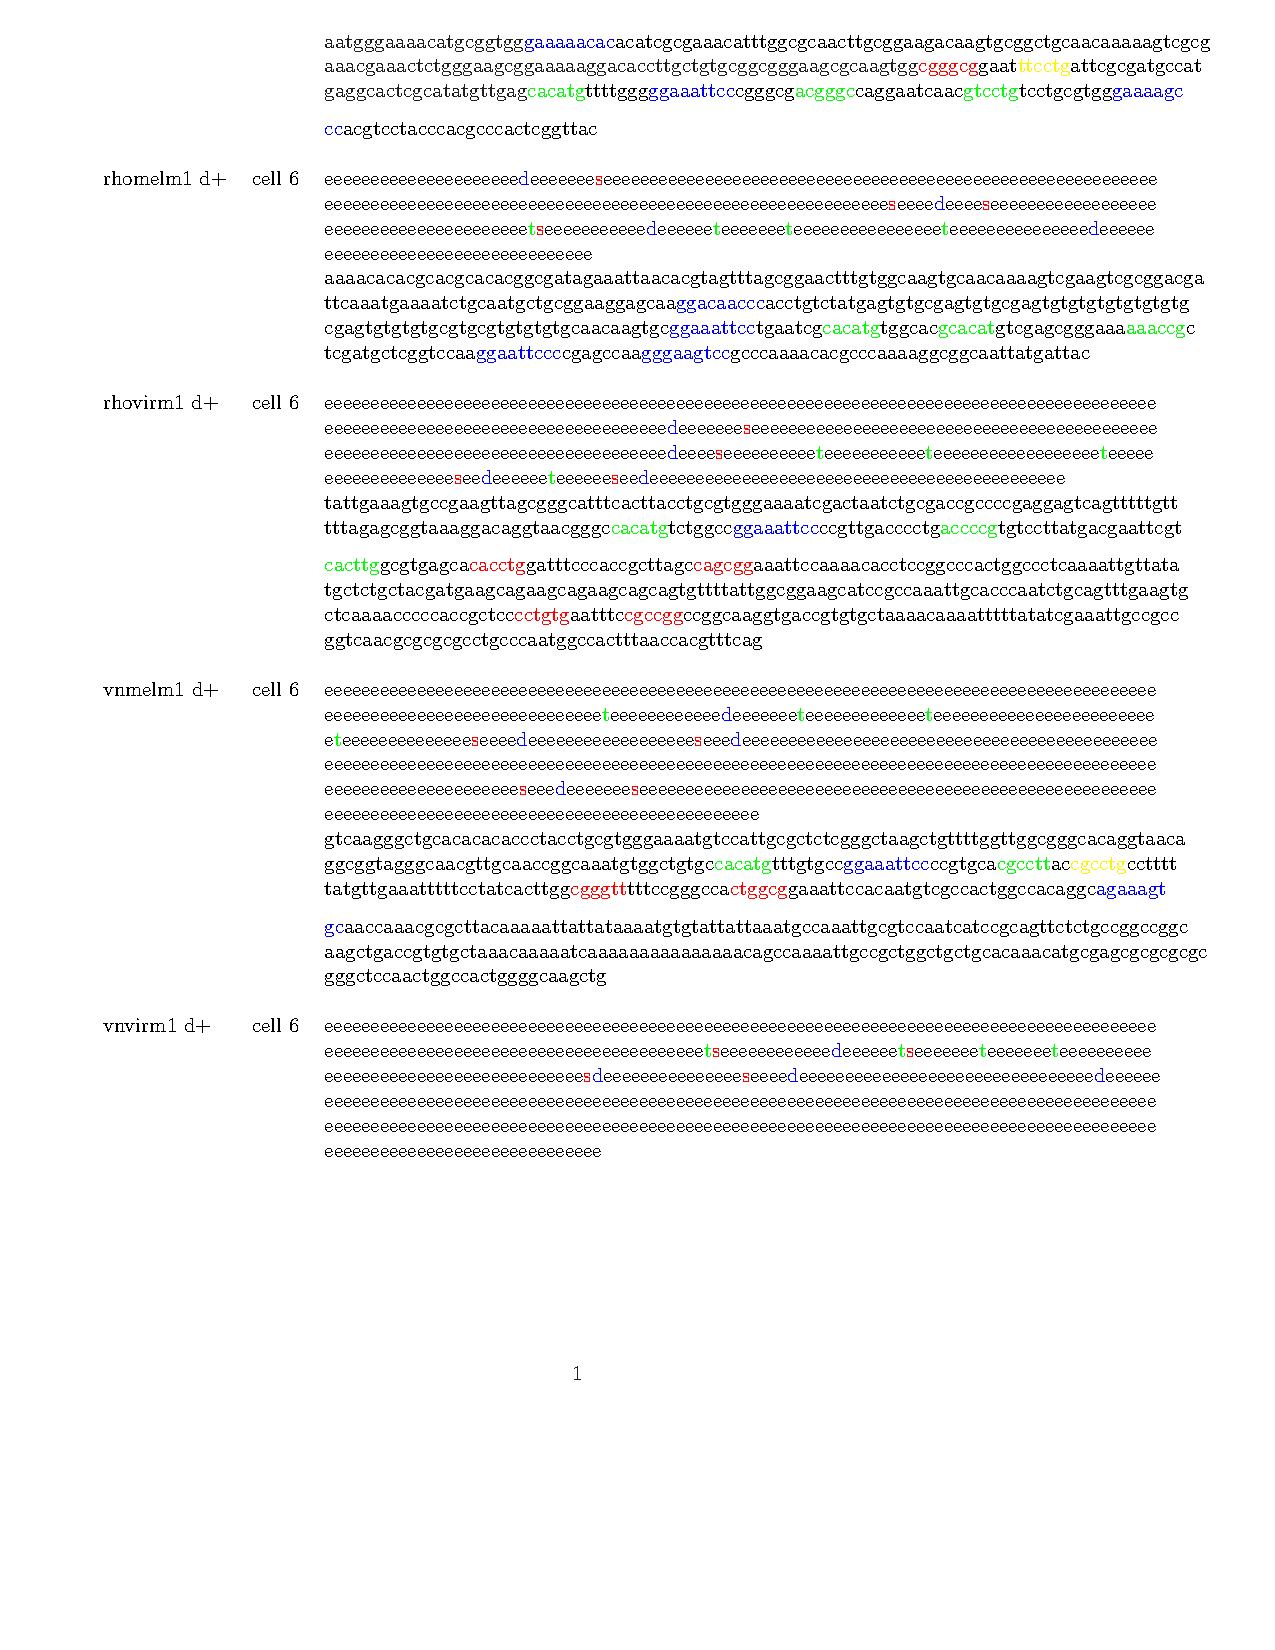
\includegraphics[height=1\textwidth]{annc}\\
  \caption{Here the target gene is denoted in the left column, where, where the second column contains d+ to denote an in increase (+) in the Dorsal (d) gradient along the DV axis, and the cell along the DV axis used for extracting concentrations for the annotation model MAP is denoted in the third column.  Twist site's are annotated green, Dorsal blue, Snail red, and brown denotes overlaps. }\label{annc}
\end{figure}



% not used \section{Discussion and Background on Robustness}
\subsection{Morphogen Gradients and Developmental Robustness}

Given a morphogen distribution over one spatial dimension, one can determine how sensitive the thresholds of the target genes are to perturbations of the morphogen distribution.  This is discussed in Alon's text in chapter 8 "Robust Patterning in Development" \cite{designp}.  Here we will reproduce Alon's derivations for producing a morphogen profile ( distribution ) and his analysis of whether this profile is robust, but we will do so in the context of the morphogen Bicoid and its robustness probe Hunchback, where similar analysis was done by Gregor and Houchmandzadeh \cite{pmid17632062}\cite{pmid11845210}.  Our analysis starts with a transport equation for the morphogen.
\begin{equation}\label{}
    \frac{\partial M}{\partial t} =  D \frac{\partial^2 M }{\partial x^2} - F(M)
\end{equation}
Here $F(M)$ is a function of the morphogen concentration and represents the degradation of the morphogen.  Notably missing from the equation is the production rate of the morphogen, as assumed from Gregor and in Alon's text the morphogen is assumed to be in steady state\cite{designp}.  Hence the time derivative is zero, and one can determine, or declare, the morphogen concentration by the boundary conditions:
$
    M(x = 0) = M_0 $ and $  M(x=\infty) = 0
$
 It is important to conceptually see what these conditions mean, since thermodynamic equilibrium in diffusion processes would lead to a morphogen distribution that is uniform over space, which we're about to see is not the case for our problem because a uniform profile occurs only if the system does not have sources and sinks.  Here we're assuming some source, a constant source such as ribosomes translating Bc mRNA at position x=0, and we are assuming a sink by the proteasome degradation of the Bc protein at $x=\infty$. \footnote[1]{ the idea that Bc mRNA is localized at x=0 was recently shown false, it was shown that Bc mRNA is also diffusing and closely follows the Bc protein profile, but for our discussion we'll assume that Bc is translated into protein at x=0 and then diffuses, and all of this is captured by our boundary condition.}
The Diffusion constant D determines the \textbf{absolute} length scale of the problem, which creates a problem for patterning mechanisms if the embryos have large variations in their size, since an intricate \textit{scaling} mechanism would be required, as diffusion is based on absolute length scales, this is discussed by Gregor and by Crocker \cite{pmid18328473}.  Assuming the variation of the embryos length is negligible we need to see how the scale of the problem is established. Alon's analysis starts with a linear degradation mechanism $F(M) =\alpha M $, where upon solving the PDE given the morphogen is in steady state, one arrives at:
\begin{equation}\label{ss}
    M(x) = M_0 e^{-\frac{x}{\lambda}}
\end{equation}

where $\lambda = \sqrt{\frac{D}{\alpha}}$, clearly when $x=\lambda$ the morphogen has reached a concentration of $\frac{M_0}{e}$, which is only about 33\% of its max, and after $2 \lambda$, the morphogen has reached a concentration of $\frac{M_0}{e^2}$ in general:
\begin{equation}\label{}
    x = \lambda, 2\lambda, .. n \lambda
\end{equation}
then
\begin{equation}\label{morpscale}
    M = \frac{M_0}{e},\frac{M_0}{e^2},..\frac{M_0}{e^n}
\end{equation}
 Using 'units' of $\lambda$ is not only useful for seeing how the morphogen decays as a function of absolute length, it is in fact the units the morphogen uses to create patterns, as when one anthropomorphizes the morphogen, they realize that the morphogen can not reproducible 'make' patterns on any scale other than $ \lambda $, where reproducible means comparing the patterns \textbf{between} embryos.


  \subsection{Fine patterns}
   Let's see if the morphogen 'can create' a fine pattern on the scale of $ 1 \mu m = $ when $ \lambda = 10 \mu m$. Now the morphogen creates the pattern by binding to the Hb promoter and stimulating Hb expression, so the Hb expression as a function of space is the 'pattern'.  This is denoted by figure \ref{shift}.  In drosophila the x axis (the Anterior Posterior axis, major axis of the elliposdal embryo) is about 500 $\mu m$ and each nucleus is separated by about 10 $ \mu m$, since the pattern here is referring to the expression of Hb as a function of nuclear position, we see that $ 1 \mu m$ doesn't even make sense, since the smallest unit of our problem is $10 \mu m$,  So let's fix our ill-posed question to the morphogen trying to make a pattern over  $ 10 \mu m $ where $ \lambda =100 \mu m $.  Now to determine if a pattern can be created all we need to know is if the Hb promoter can detect (distinguish) Bc concentrations that are separated by $ 10 \mu m $  (two neighboring nuclei).  Well the answer is simple, \textbf{yes}, if we use the Hill model \eqref{segcon2hb}, to represent Hb's detection mechanism, then clearly the promoter can detect \textbf{any} concentration of Bicoid, and clearly any desired pattern could be produced  (To determine the pattern one simply defines a Bicoid concentration as the start of the pattern (i.e. a 'threshold concentration', M(x)) and and then inverts the Hill equation to find the Bc concentration and position, which come from equation \eqref{ss}).
 \begin{equation}\label{segcon2hb}
    \frac{[Hb]}{[Hb_{max}]} = \frac{1}{1 + e^{ -(w_{0} +  \left< n_{Bc} \right> w_{Bc}})}
\end{equation}

 But, we want to explore this problem from the perspective of robustness, that is if the Bc concentration deviates from its ideal profile for whatever reason (e.g. the mother laid less functional bc mRNA because only one of her bc alleles is functional (heterozygote ), or a slight variant of mRNA are laid in the oocyte etc..) , then what would happen to our Hb profile.  In this sense, one may loosely say that we are interested in knowing if a nonrobust input can still be transformed into a robust output \footnote[2]{for thermodynamic modeling (fractional occupancy) this question is approximately answered by taking the derivative of the model $<N_{mRNA}>$ with respect to the input concentration that is varying, one will see that the effect is only at the border due to the form of the model}.

  A formal measure of this (robustness) is defined by Alon as the 'positional shift' that is by how many microns $\delta $ does our pattern shift.  To determine the function $\delta $ we need to perturb the production rate M (i.e. the boundary condition at x = 0) from $M$ to $M'$, then one can see $\delta $ from the graph in figure \ref{shift}.  When analyzing these equations, keep in mind that the Hb concentration is captured by the concentration of the morphogen [M], so M(x) and M(x') represent the same Hb concentration.
  \begin{equation}\label{inverse}
    d x = \frac{d x }{d M} dM
  \end{equation}

\begin{equation}\label{solvex}
    dx = \delta = x - x'
  \end{equation}
  inverting equation \eqref{ss} we can isolate the position, hence solving for x:
  \begin{equation}\label{}
   x = \lambda \log{\frac{M}{M(x)}}
  \end{equation}
  now if we change the boundary condition to M', and solve for x', which represent the new border position of Hb expression:
  \begin{equation}\label{}
  x' = \lambda \log{\frac{M'}{M(x')}}
  \end{equation}
  now we have the pieces to calculate $\delta$,
  \begin{equation}\label{}
     \delta = \lambda \log{\frac{M}{M(x)} }- \lambda \log{\frac{M'}{M(x')}}
  \end{equation}
  since M(x) = M(x'), we arrive at:
  \begin{equation}\label{}
  \delta =  \lambda\log{\frac{M'}{M}}
  \end{equation}

\begin{figure},
  % Requires \usepackage{graphicx}
  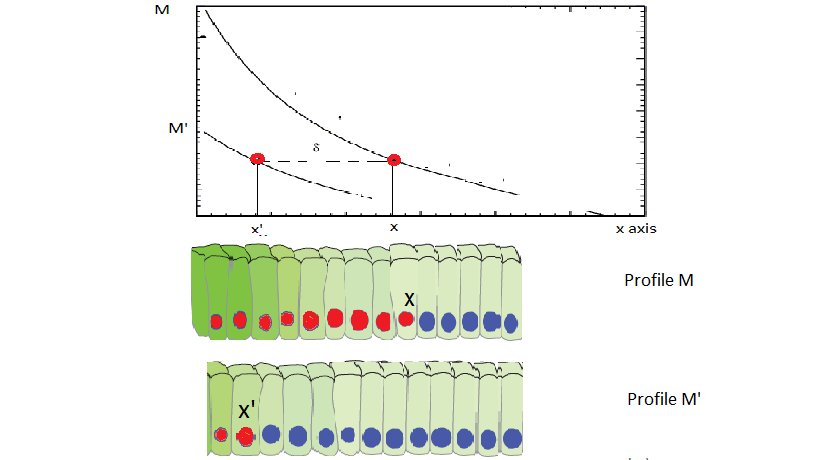
\includegraphics[width=1\textwidth]{sourcegraph}\\
  \caption{the green gradient represents the concentration of Bicoid and the orange nuclei denote Hb expression, while blue nuclei represent no Hb expression.  This figure was modified from figure 1 of \cite{pmid20066104}, and Alon's text\cite{designp}.}\label{shift}
\end{figure}

  Now that we know $\delta$ we can analyze why $\lambda$ is the effective length scale.  For example, let $M' = \frac{M}{2}$, then $\delta = \lambda log(\frac{1}{2}) \approx .7 \lambda $.  Recall, we wanted to find if the morphogen can create a pattern over $10 \mu m$, which was effectively the finest pattern since  $10 \mu m$ is the spacing between two cells or nuclei, but $.7 \lambda $ is a shift of 7 nuclei!  Clearly, for our problem, if the production rate varies by a 50\% reduction (as seen for classical heterozygote experiments,where one allele is lost), a precision on the order of the spacing between nuclei is not possible.


    Hence, the idea, of 'relevant length scale' for our problem can be understood from the perspective of what happens due to natural variations in morphogen gradient.

   % although other problems may have other reasons for defining their length scale (for example an optical wave moving through a lattice of atoms may compare the atomic spacing to the wavelength of the wave, where for wavelengths much shorter than the atomic spacing there may be no perturbations since the atoms 'see' both up and down fields, canceling any affects on the atoms movement.)\\
\par
Determining if a pattern is 'robust' to the morphogen's gradient (nearly independent of the morphogen's production rate) or if the pattern is 'fine-tuned' (extremely sensitive to any variation of the production rate) is an important problem in studying morphogen gradients - the parenthetical definitions both come from Alon's chapter 7 'Robustness of Protein Circuits'.

From our analysis, we see that the two goals of \textit{attaining} 'robust' outputs, while \textit{maintaining} a 'fine' pattern for the output are at odds with one another, there is a tradeoff.  The more robust we make our output to variations of the input then the less the module will be able to distinguish concentration differences of the input, and hence will not be able to produce a 'fine' pattern.  However, great attention has been given to 'combinatorial' regulatory mechanisms, in this sense one can imagine that noisy inputs do allow for robust and fine tuning, but the robustness is with respect to 'redundant' inputs \footnote[1]{For example, if two activators are both sufficient for transcription and both bind to the module that determines the output then random noise in one activator can clearly be compensated for by the other input}.  This can for example be achieved through cooperativity, or rather than robustness from combinatorial inputs, the promoter may have redundant binding sites for a key activator, thereby reaching the minimal number of morphogen to be bound for maximum expression.

For example Let us model the  border of rhomboid expression as a function of cooperativity.  Then we can ask how robust is the border with respect to variations of the concentrations of Tw and Dl \footnote[2]{here we should be careful as Tw concentration is a function of Dl concentration, hence their noise is correlated, although less so at the dorsal border of the neuroectoderm, for simplicity we'll assume the noise in uncorrelated}.

If we apply the analysis of Alon to the rhomboid gene\footnote[3]{tissues are defined by their gene expression, so we our analysis is simply to find the threshold T, (the border concentration) of rhomboid}, which is in this case activated by two morphogens $M_{dl}, M_{tw}$ we see that if we wish to apply 'thermodynamic modeling' it doesn't matter what the actual profiles of the Dl and Tw look like, all we need to do is vary these two concentrations simultaneously and analyze its effect on the model $<N_{mRNA}>$.  Using the fact that $ < ( \delta n_m )^2 > = \frac{\partial Z}{\partial n_m }$ one can check by simulation that $ < ( \delta n_m )^2 >= \sqrt{<n_m>} $.  
For example, the Rhomboid expression at the dorsal border:
\begin{equation}\label{}
    <N_{rho} > = \frac{1}{1+e^{-<n_{dl}>w_{dl} + <n_{sn}>w_{sn} -<n_{tw}>w_{tw}}}
\end{equation}
the w's are the parameters to be fit, and the n's represent the average occupancy of each protein on the promoter.
It is known that twist alone is not sufficient for transcription, so we can set $w_{tw} = 0$, furthermore the dorsal border of rhomboid is well beyond snail's expression pattern, hence there will be no snail occupancy there, so $<n_{sn}>=0$.  Leaving:
\begin{equation}\label{}
    <N_{rho} > = \frac{1}{1+e^{-<n_{dl}>w_{dl} }}
\end{equation}
Therefore the variance in $<N_{rho} >$, which we'll label as $\sigma_{rho}$ will be roughly the range of expession:
\begin{equation}\label{}
 \sigma_{rho}  = \frac{1}{1+e^{-(<n_{dl}> +\delta n_m ) w_{dl} }} - \frac{1}{1+e^{-(<n_{dl}> -\delta n_m ) w_{dl} }}
\end{equation}
Once sigma is known one can then determine by how far the threshold concentration of Rhomboid ($M(x) = T $) has shifted in terms of cells, in the sense that $<N_{rho}^x > \pm \sigma_{rho}^x$ yields the two new expected values of Rhomboid, and one can simply compare these with the expected Rhomboid profile. (i.e.  $ <N_{rho}^x >- \sigma_{rho}^x  = <N_{rho}^{x'} >$  and $x-x' = \delta$ the shift.  Since $<n_{dl}>$ is related to the occupancy of twist, $<n_{tw}>$, this implies that the variance in dorsal occupancy $\delta n_{dl}$ captures how both dorsal and twist variations cause shifts in the dorsal border of rhomboid.  Another way is to simply look at that matrix element within the Hessian:
\begin{equation}\label{}
    \frac{\partial^2 <N_{rho}>}{\partial M_{tw} \partial M_{dl}}
\end{equation}
\subsection{Definition of Border and Production Rate}

Alon defines a transcription network as a set of nodes (target genes) and set of edges ( inputs to Hill function ).  The inputs to each each node are the three parameters that define the Hill function ( n, K ,$\beta$ ), where n is the Hill coefficient, K is the equilibrium constant of the transcription factor activating or repressing the node \footnote[1]{ $\beta$ is the production rate ($V_{max}$) in Michelis Menten kinetics, that is maximum expression level}, and $\beta$ is the production rate of the gene.  Hence for a particular gene, which has mRNA concentration Y, one would have the following equation defining the gene's dynamics:
  \begin{equation}\label{}
    \frac{d Y}{d t} = \frac{\beta_{Y} }{ 1 + X/K} - \alpha
  \end{equation}
  Here X is the concentration of an activator transcription factor and K is the equilibrium constant for the the factor X to its binding site, (for a repressor input simply inverse X/K), and $\alpha$ is the degradation rate of the mRNA or (protein product depending on what Y represents).

  Clearly for any gene (node) $\beta$ is constrained by processtivity (the maximum translocation rate, $V_{max}$, of POLII along the gene, which is doubled with $10^{\circ}$ increase in temperature (ref Davidson), hence $\beta \in [0,V_{max}]$, furthermore since each gene, g,  will have its own production rate, we can say $\beta_g \in [0,\beta_{max}]$.

  Now from this description all of the information about the max production rate for our model (i.e. for a specific gene ) is encoded inside of the sigmoidal function of the w'sbecause the max production rate of the entire network is $\beta_{max}$, and because the model $<N>$ is divided by $\beta_{max}$ ( similar to Gregor's [Hb]/[Hbmax]) \footnote[1]{Sinha's lab noted that the correlation coefficient (one possible form of the objective function use to fit the parameters of the network) is scale invariant, hence they create a model where $\beta$ is a free parameter for EACH gene.  This is exactly the way Alon describes the network (where each gene gets its own $\beta$, however i prefer to not do that because that changes the meaning of the 'border', and hence the meaning of the ws in the sigmoidal.}  This means the maximum expression, in our model this is 1, is at  $\alpha/ \beta_{max}$ (assuming steady state).  Now as we vary the genes in the network, if we assume $\alpha$ is fixed\footnote[2]{ since our reporter for each gene (or module) is LacZ, it is safe to assume the degradation rate of LacZ mRNA and protein is roughly the same}  then for different steady state levels, it follows that $\beta$ must be varying (i.e. decreasing from $\beta_{max})$, hence there is a rule, which maps our sigmoidal function of the w's to $\beta$,  (the operation is not one to one due to saturation of the sigmoidal function, assuming we don't have infinite precision).
\par
In our description of the profiles we have assumed that some profiles are not producing at $\beta_{max}$, that is we have lowered the level of gene expression because the level is lower then a reference gene which give $\beta_{max}$ (that is all genes whose expression level is at 1).
\par
In assigning different expression levels ($\beta$), one is not affecting the \textbf{border} of the expression (i.e. the parameter K ), as in this model the parameters ($\beta$ and K ) are independent.  Hence some profiles which have their max expression levels below 1/2, do not have a border.  However, as pointed out by others, one could imagine a step wise (ladder) function, where there are multiple borders (i.e. the level =1 is not the max anymore).  For example we could assume an expression level of 2 as the max:
\begin{equation}\label{}
    f(Y_{ss}) = \beta_1\theta(K_1) + \beta_2\theta(K_2)
\end{equation}
Here $Y_{ss}$ is the steady state concentration, and $theta$ is the step function, hence once X is above $K_1$, the level jumps to $\beta_1$, then it stays at that level until X reaches $K_2$, at which point the level jumps to $\beta_1 + \beta_2$.  Actually this equation isn't properly written as one should start from the dynamic equation (with degradation) and solve, but the idea still holds, the borders are ($K_1$ and $K_2$), which allows for lower expressing modules to have a well defined border (K).

If we assume our set of target genes $\textbf{G}= {g_1,g_2,..g_n}$  (i.e. regulatory modules or sequences $\textbf{S}^{crm}$ in our Data set $\textbf{D}$), follow the production rate relation: $\beta_g \in (0,\beta_{max})$,  then using the Segal/Hill equation (equation \ref{segcon2},
 \begin{equation}\label{}
    <N_{g}> = \frac{1}{1 + exp{-(w_o +\sum_i<n_i>w_i)}}
 \end{equation}
 we can linearize it to solve for the w's:
 \begin{equation}\label{}
    \log{\frac{<N_{g_1}>}{1-<N_{g_1}>}} = w_o +\sum_i<n_i>w_i
 \end{equation}

 if we assume the factors $i$ govern all n genes then we have a matrix equation:
\[
\begin{pmatrix} \log{\frac{<N_{g_1}>}{1-<N_{g_1}>}}\\ \log{\frac{<N_{g_2}>}{1-<N_{g_2}>}} \\ \vdots \\  \log{\frac{<N_{g_n}>}{1-<N_{g_n}>}}\end{pmatrix}=
 \begin{pmatrix}
   1& <n_{X1}^{g_1}> & <n_{X2}^{g_1}> & <n_{X3}^{g_1}>  \\
   1&<n_{X1}^{g_2}> & <n_{X2}^{g_2}> & <n_{X3}^{g_2}> \\
    \vdots & \vdots & \vdots \\
   1&<n_{X1}^{g_n}> & <n_{X2}^{g_n}> & <n_{X3}^{g_n}>
 \end{pmatrix} \begin{pmatrix} w_0 \\ w_1 \\ w_2 \\ w_3 \end{pmatrix}
\]
Here we can use all (infinite if continuous) possible points along the profiles ($<N(z)>$ where z is cellular position \footnote[1]{

recall that the occupancies are function of concentration: $<n_X> $, and hence are a function of position along the tissue.  If we have 40 cells that we measure $Y, X_1,X_2,X_3$, then and if we n genes, then we'll have n*40 equations, and hence n*40 rows in our matrix.  Many of those equations will have the same value for Y, and hence can be set equal to each other, this is a consequence that there are many possible occupancies that lead to the same value of $\chi$, however if we fix $chi$ to be say 4,5,6,7 then we have a system of 4 equations, if we select one gene that has all these values reached at some point along its profile we'll have:
\[
\begin{pmatrix} 4 \\ 5 \\ 6 \\ 7\end{pmatrix}=
 \begin{pmatrix}
   1& <n_{X1(z1)}> & <n_{X2(z1)}> & <n_{X3(z1)}>  \\
   \vdots & \vdots & \vdots \\
1& <n_{X1(z4)}> & <n_{X2(z4)}> & <n_{X3(z4)}>
 \end{pmatrix} \begin{pmatrix} w_0 \\ w_1 \\ w_2 \\ w_3 \end{pmatrix}
\]
where z is variable position along the profile, evaluated at 4 different positions, z1,.z4.  In this case it is reasonable and in fact mandoratory that the occupancy change from one equation to another.  However, what if we collected 4 positions, that all had identical values of $\chi$?}

) to solve for the w's, furthermore we also see that the points corresponding to $$<N_{g}> =\begin{cases}0  \\ 1 \end{cases}$$ lead to singularities, which is not surprising as there are infinite combinations of w's that in the limit give 0 or 1 for the sigmoidal function (another way to think of the 1,0 solutions, is that they have lost information, as there are multiple inputs that lead to 1 or 0).

\par

However if $<N_{g}> \in (.1,.9)$, then our matrix equation is well defined.  (Here there may be multiple ways to to yield these solutions too, as are may ways to generate a fixed number from a sum of 3 integers). In particular if we collect all the genes that have a border (i.e.  $<N_{g}> = .5$, which is analogous to X=K in the above discussion, and for our case it is like saying the gene's activator occupancy $<n>$=K) we then will have a subset of \textbf{G}, which yields a homogeneous system of equations:



\[
\begin{pmatrix} 0\\0\\ \vdots \\ 0\end{pmatrix}=
 \begin{pmatrix}
     1&<n_{X1}^{g_1}> & <n_{X2}^{g_1}> & <n_{X3}^{g_1}>  \\
   1&<n_{X1}^{g_2}> & <n_{X2}^{g_2}> & <n_{X3}^{g_2}> \\
    \vdots & \vdots & \vdots \\
   1&<n_{X1}^{g_m}> & <n_{X2}^{g_m}> & <n_{X3}^{g_m}>
 \end{pmatrix} \begin{pmatrix} w_0 \\ w_1 \\ w_2 \\ w_3 \end{pmatrix}
\]

Now if we imagine m = 3, we can make some important analysis (for m $>$ 3, we can use least squares to solve  w \footnote[1]{ Least Squares gives an analytic solution to the minima, and this minima for a linear equation can be shown to be the global minima, for the situation with error in both inputs and outputs, I believe one finds that there are multiple roots and hence multiple minima, but the number of minima are small, hence one can exhaustively look at all the minima and simply find the smallest (the global)}).  If m=3, we have a system of 3 homogeneous equations, with 3 unknowns (w's).  If our system is linearly independent, then the w's must be zero, as that is the unique solution for a homogeneous system that is linearly independent ( if this is true for m =3, it obviously holds for m $>$ 3, which means adding more genes doesn't help us find nontrivial w's).  \\
\par
Furthermore, if the variables are linearly independent all from one gene, then this indicates a method to see if the idea of putting multiple genes in the network makes sense (i.e. does each gene have its own set of ws, or are the ws governing the entire network).  As adding more genes (which will increas m) will then cause the matrix equation to stay consistent or the system will be inconsistent.  \\
\par
Clearly the idea of 'Least Squares' already indicates the system of equations is inconsistent, and hence one is to maximize the projection (parallel component) of the vector \textbf{Ax} onto the data set \textbf{y}, thereby minimizing the perpendicular component (i.e. the deviation ($\sum A_{ij} x_j - y_i$).  However, one could imagine creating a statistical test, like a t test, where the average error component is the max of measurement and biological noise, then one can add a new gene to the matrix calculate the error and then could calculate, then one has a statistic which they can use to calculate the p value.\\
\par
This is consistent with the idea of the network being completely governed by the occupancies.  This is basically telling us that there is only one master gene (that's why there is only one w vector), and that that gene always expresses when the activator occupancy goes from j to j+1 (this was an observation pointed out by William Wedemeyer in a discussion on the pseudoinverse).
\par
So if the factor's occupancies are linearly dependent\footnote[2]{ the $<n>$'s i think would be linearly dependent because the idea that the occupancy goes from j to j+1 for activation (when crossing the border), means there is an equation relating the occupancies, namely $\sum_i<n_i>w_i = j+1$, where $j+1$ is playing the role of K}, then least squares will not work, as the design matrix doesn't have an inverse if it is underdetermined, however, the method of svd, allows for this, by using the pseudo inverse (this is also known as the Moore Penrose inverse).  Regardless, it is algebra, one inverts the matrix, which can be done by almost all linear algebra packages. If we have m $>$ 3 and assume our system is undetermined, then we our left with finding a nontrivial solution in the null space (as we obviously don't want all the w's zero).  This means that there are infinite solutions to the w's (well there would be only one normalized solution in the null space). 
\subsection{Uniform Shifts and Scale Invariance}

Scaling laws are relations between an attribute of a system and the size of the system (the size is the scale like length, mass, volume).
Power laws (e.g. polynomical equations relating the attribute to the size), are important in biology, because they indicate scale invariance.  That is the system is able to preserve the form of the relation as the scale varies.  In this sense scale invariance is a bit of a misnomer, it would have been better to say the equation is invariant, but such is tradition.
Work by Erives lab has shown that patterns are scale invariant (so the pattern width gets wider as the length of the embryo gets longer according to some law, possibly a power law).  This was achieved by looking at different sized embryos (different because they were different species of flies).  Interestingly they noted the pattern's modules grammar is NOT invariant.  That is the module changes (evolves by genetic mutations) to compensate for scaling.  Scaling laws are by nature very coarse grain, scaling laws do not tell one anything about the detailed mechanism within a object.  However, Erives work (or his student Crocker's work) in some sense linked the coarse with the fine details.
%
%For larger sized embryoes one can ask if the pattern has expanded, or if the absolute number of mrna has increased (presumably a consequence of expanded pattern),  if the nuclei are larger due to larger genomes etc.. then the expanded pattern may be isometric (pattern width divided by mass is a constant when one varies mass, hence the ratio is a constant, hence the relation w = km^a has 'a' equal to one, where w is width m is mrna (normally mass) 'a' is the allometric exponent, and k is the allometric constant. (ref answeres.com, wiki).  Isometry is the null hypothesis for scaling relations.
%
%If we have isometry for positional morphogens, then there are problems for explaining how the enhancers deal with such issues.  For example imagine one doubles the width of the embryo, than isometry predicts p = 2p'  where p' is the original pattern width, now if the number of nuclie are constant (2^14 ncs no matter what species) then presumably the the new width still occupies the same number of nuclei, the nuclei are just bigger or have a larger internuclear spacing ( 8 um for melanogaster at nc14, so maybe it just increases to 16um for a larger embryo).  If the time of development or some other mechanism does not occur than one could expect that the larger embryo would have less internuclear mRNA (cytoplasmic) since the absolute quantity would be the same..
%
%From wiki: " Isometric scaling occurs when changes in size (during growth or over evolutionary time) do not lead to changes in proportion."
%From wiki "size means dimensions such as length width height surface area, volume.
%the square-cuble law indicates that  an organism that doubles length will find its surface are quadruple, while volume and mass will increas by a factor of eight!"  This is interesting for maternal genes, do they increase 8 fold when length increases?, something increase 8 fold what is it?
%
%One would expect that their is negative allometry for rho expression since, the number of cis-elements is fixed (and therefore show negative allometry), hence the only way to get back to isometry for an expanded pattern is for the promoter to fire at a stronger rate, or for the nc time to change allowing for more steady state tf-crm interaction, that's important to change up the time since the spatial averaging is affected by the increased internuclear distances nuclear distances.  I think i read the the development is longer for larger embryoes (find ref).  This is an important relation the one of scale invariance being related to time, it may be that the transformation for invariance must not only be kx, but also kt, that is when scale changes so does the time scale.  cr. maxwell equations, scale invariance.
%
%scaling is essentially, using different units, if x -> 100*x, that's like saying we'll plug in our function cm instead of m, so all of our measurements have to be scalled by 100, since there are 100 cm per meter.
%
%the amount of scaling refers  to the alometric exponent, and it should be noted that power laws (polynomial equations as above, or distributions with a long tail) and exponentail exp(kx), both exhibit skaling since f(kx) proportional to f(x), as:
%$exp(k5x) = f(5x) = f(x)^5, actually this system does not exhibit scaling. but f(5x) = k(5x)^a = 5^a*f(x)$ which is proportional to the original, meaning the shape of the function stays fixed.  Note, gaussians, do not exhibit this bahavior, therefore the shape changes when the scale changes, that is, gaussians are not scale invariant: (figure:  gausScale), unless the width or shape parameter sigma is heteroscadastic over all scales, then a change in units, will cause a corresponding change in sigma, actually since the factor x/s is unitless it automatically is scale invariant!  Actually the problem is one like Maxwell's equations, the function is a two parameter or two dimensional function, with respect to x and s..  just as maxwells requires x -> ax, and t -> at.
%
%another problem of scaling is that for larger embryos with absolute quantities of bicoid constant, this doesn't make sense for Dorsal, as larger embryoes will require larger genomes that require larger nuclei the larger nucle in turn will require more activated toll receptors on the vitellane membrane, which means more spatzle will be required, in order to activate all of these receptors.  Now an increase in devo time, and especially sampling time of the genome, may compensate these factors.
%two problems, there are conflicting lines of evidence of that there are actually more nuclei in larger embryos, and that the devo times are the same.  This is same old bus from bio, one states knowledge as if its truth (since they're an authority) but in reality (in quantitative) they don't know what their talking about.
%
%heterochrony an idea of ernest hackel in 1890 mentioned that changes in rates can effect development, leading to changes in size and shape. pedomorphosis is the retention in adults of juvenile phenotypes, where the juvenile phenotypes can readily be adapted to change, while specialized adult features are resistant to change.  neoteny is also the retention of juvenile in the mature.
%////
%Scaling:  Direct quotes, and paraphrasing from the following:
%"Diffusion and scaling during early embryonic pattern formation", 2005, Gregor
%Using diffusion equation one sees that the length scale leads to nonscaling behavior, that is once the solution is solved the relavant constants are not dependent on the scale of the system, the constants, like the decay term in exp(-xt) the decay term 't', this constant is Dt' , which is the diffusion constant and the lifetime of morphogen.  If neither the lifetime nor the diffusion constant depend on the length scale of the system, then clearly the system will have no way to scale the gradient when the overall system (egg length) changes size.
%"Scaling of Gene expression profiles" page 18405, "Diffusion-based models provide no natural mechanism for generating spatial patterns that scale with size of the egg."  "the diffusion and biochem reactions, the diffusion constant and reaction rates determine an absolute length scale., thus when the size of the system changes, the spacing of the pattern elements would remain fixed"
%
%Mechanisms for scaling (page 1405 section "Scaling of gene expression profiles")
%two mechanisms for generating scaled versions of these profiles in species with larger embryos:
%1. the Bcd gradient could stay the same, and the cis-acting control sites of downstream genes could have adapted over evolution so that specific genes are activated by lower concentration of Bcd in species with larger eggs.
%2. (the alternative hypothesis), the Bcd gradient itself could scale, while the readout mechanisms encoded in the control sites of downstream genes are conserved across species".
%scaling is essentially, using different units, if x -> 100*x, that's like saying we'll plug in our function cm instead of m, so all of our measurements have to be scalled by 100, since there are 100 cm per meter.
%
%To distinguish the possibilities, they examined Bcd protein profiles from stained immunofluorescently, in L sericata, D mel,
%they noted Houchmandzadeh 2002, to show that the considerable  variability within one species jived with Houchmandzadeh's results! (last sentence page 18405 and figure 3A).
%
%Conclusion for how scaling of Bic gradient achieved: lambda = Dt, and of these two options, D is changed by 'effective transport parameter b', or t is changed by varying degradation machinery or someother species specific lifetime  adaptation.
%
%" of the many possible mechanisms for scaling, the only one taht is consistent with our data is variation in the effective lifetime of the Bcd protein itself."
\subsection{Molecular basis for Robustness of Morphogen gradients}

%Seeing that the linear degradation term in the morphogen PDE did not lead to a robust solution, a different functional form is needed for degradation, (assuming the Diffusion Coefficient and
Alon and Eldar's work show that a robust profile would require a degradation rate that is a nonlinear implicit function of space, $ F(M) = -kM^2$, a power law for the degradation is worked out in Eldar's paper that shows robustness\cite{pmid12239569}.  Furthermore Gregor showed that among different Dipterian species that have different sized embryos the domain on the Bicoid protein that is targeted for degradation has been fine tuned by evolutionary mutations thereby allowing for a scaling mechanism between the different sized embryos that leads to a robust profile for Bicoid.  Gregor also analyzed the possibilty that target gene's cis regulatory modules may be fine tuning the Bicoid binding sites to achieve a mechanism to scale the patterns in larger embryos\cite{pmid16352710}\cite{pmid16352710}.  Crocker analyzed cis regulatory modules of Dorsal and Twist targets and found that the spacing between Twist and Dorsal binding sites had varied, by testing the effects of this variation in a \textit{in vivo} study they showed that changing the spacing (the number of base pairs between Dorsal and Twist sites) changed the target profile's anatomical positional border (the neuroectoderm- dorsal ectoderm border of the embryo), hence explaining the scaling mechanism for different sized embryos by the architecture of the enhancer.\footnote[1]{Crocker's assumptions assume same number of nuclei at nc14 = $2^{14} \simeq 16000$, however there has been indications that the number of nuclei scale with size of embryo, indicating nuclear cycles may not be completey synchronized, or there are more maternal nuclei in the syncitium (the chamber that holds the egg) than the initial mother's egg (haploid nucleus).\cite{kreitman} seeing that there is variation in the number of nuclei, that indicates that for target genes making decisions at nc9, then by nc14 the width, w, of the expression pattern will not minimally be $w = \log{\frac{2^{14}}{2^9}} =5 $ nuclei as indicated by Bialek in his response to Sven Bergman's paper on pre-steady state decoding\cite{Response}\cite{pmid17298180}. } 

% not used \input{pwminput}



%\subsection{Abolition, single site knockouts}
%\subsection{Multiobjective}

%\input{alonrobust2}



\newpage
\section{Conclusion}
The MPA annotation model developed here was used in conjunction with the OR gate for Dorsal binding sites ( DC and DU PWMs).  The OR gate was designed to be sensitive (it is more likely to call a positive hit than its component PWMs), while disregarding the pitfuls of specificity (a false positive picked up by just one component detector will be declared a positive for the OR gate, even if the majority of component detectors declare the site a negative.).  The high sensitivity of the OR gate used in conjunction with the the MPA annotator (which is designed for high specificity),  yields a highly effective bioinformatic tool for discovery of binding sites.  Annotation of CRMs at half max occupancy of the Basal Transcription Apparatus (the transition from the boolean 0 to 1 expression), reduces the likelihood of picking up binding sites that are nonfunctional and hence misclassified as a 'hit' in the annotation process, since high occupancy of BTA could result from many binding sites that are not critical to get the initial switch.

 The occupancy model generalizes over binding sites, in that the input to the model is an enhancer sequence, not a list of binding sites.  So a priori one does not know what binding sites will be selected, rather the physical control parameters (concentration, binding energy, protein-protein interactions) determine what is a binding site.  In this sense the MPA annotation model could be thought of as generating a fixed number of binding sites as part of its output.  This is a contribution to the field, which i point out Segal said specifically their model could not address at this level of detail, they could only make statements about the numerical values of cooperativity quenching.  With this being said one could judiciously choose parameter values to reconstruct the exact engineered enhancers (which in a sense we did for our last experiment), but of course, we wish to find parameters which are consistent with not just one construct but the entire GRN.
 
 Much of the analysis is about experimental design, as experiments are not only necessary to test theory, but they are necessary to tune parameters for well known theories.  Binding of morphogens to CRMs is not a theory under dispute, nor is the theoretical calculation of the occupation of the morphogen's to the CRM, that's been known for many years.  What is not known is the strength and importance of the parameters controlling the occupation of morphogens on the promoter, and how much each of these in turn affect BTA binding.  This requires model design, to infer what the value of these parameters.  However, this data is not always available, hence I have shown an alternative technique, where I have tried to use low quality data from the literature to tune the parameters.  As was seen from Experiment 2, it is possible to mathematically arrive at certain conclusions reached by Szymanski (that cooperativity is necessary in the NEEs).  However, Szymanski's $6xdl$ construct is not consistent with reported parameter ranges of thermodyanmic models collected by Buchler et.al.\cite{pmid12702751}. Hence, it was necessary to adjust the thermodynamic model parameter ranges.  Possibly one could argue that one can not adjust the parameter ranges found by Buchler since they cover a broad spectrum of proteins.  Indeed, the values of the cooperativity we found in Experiment 2 are so high that is unlikely Dorsal and Twist would ever unbind once bound; albeit it is possible Dorsal-Twist dimers do occur in the nucleoplasm.  Furthermore, Szymanski and others have reported 'uniform' expression profiles in certain constructs (CRMs) that are not fully 'on' (the staining of the target gene was weak).  Such reports are not consistent with the themodynamic model for Dorsal occupancy, since Dorsal occupancy is never 'uniform' it is a gradient, like Lewis Wolpert's French Flag model of morphogens.  Hence, reconstruction of basic assumptions I have made here may be necessary to accurately represent Dorsal targeted genese in DV.      

	Lastly, the idea that one should search for the ideal positive definite Hessian at the best estimates of the parameters is incorrect for the DV network.  The elusive positive definite Hessian is only for independent parameters.  The biochemical parameters that control the logic (gene switches) governing early development have coevolved to work together to jointly regulate the DV axis, hence it is wrong to state that the parameters must be independent.  
% not in use \input{dataset}
% not in use 
 \section{Model Background}

 \subsection{Fractional Occupancy of Morphogen Binding to DNA binding Site}

The binding process is modeled using a first order rate law, where M is morphogen and B is the Binding site of DNA, and MB is the complex:
\begin{equation}\label{}
    \frac{d [MB)]}{dt}= k_{on}[M][B] - k_{off}[MB],
\end{equation}
where the brackets [ ] denote concentrations, and $k_{on}$ is diffusion limited on rate,  and $k_{off}$ is the off rate that is determined by the electrostatic interactions and will vary between morphogens.  Using chemical reaction notation, we can write the above rate law as:
\begin{equation}\label{}
    [M] + [B] \Leftrightarrow [MB].
\end{equation}
In equilibrium we have:
\begin{equation}\label{ka}
  K_{a} =  \frac{[MB]}{[M][B]}= \frac{k_{on} }{k_{off}},
\end{equation}
where the $K_{a}$ is the association constant (binding constant).
The Binding site is either occupied ($o$) or unoccupied ($u$) hence the total ($t$) amount of B is conserved :
\begin{equation}\label{}
    B_{t} = B_{u} + B_{o}
\end{equation}
From this equation one is able to construct a Binomial probability space\footnote[2]{If we encode the bound state and unbound state in the Bernoulli Random variable (i.e. 1,0) we have: $E(X) = \mu = \sum_i X_i P_i = 1 P + 0 (1-P) $} \footnote[3]{ $\sigma^2 (X) =\sum_i (X_i-\mu)^2 P_i = (1-P)^2P + (0-P)^2(1-P) = (1-P)P $ }.  The fraction of occupied binding site $B$ determines the distribution's parameter $P$:
\begin{equation}\label{}
   P = \frac{B_{o}}{B_{t}}
\end{equation}
which can be rearranged in terms of the concentrations (i.e. [MB] and [B]):
\begin{equation}\label{Zb}
    \frac{B_{o}}{B_{t}} =\frac{[MB]}{[MB] + [B]}
\end{equation}

\begin{equation}\label{}
    P =\frac{[MB]}{[MB] + [B]} = \frac{K_{a}[M]}{1+K_{a}[M]}.
\end{equation}
Again, $K_a$ is the association constant of the morphogen, $M$, to the binding site $B$.  Previously we have denoted this constant as $K(S)$, where $S$ is a DNA sequence that functions as a binding site for the morphogen. 

\subsection{Fractional occupancy of CRMs containing multiple binding sites }


Given that most regulatory sequences have multiple binding sites for multiple different morphogens one has a master equation governing the binding process, a set of coupled differential equations.  Here, again, we will assume the binding process has equilibrated, and hence we simply must enumerate the states (configurations of bound and unbound sites) of the many-binding site system.  For independent binding this is simply multinomial process (where the 'multi' aspect accounts for the different types of transcription factors binding to the CRM).  For example, for a single type of transcription factor binding, to n binding sites within a CRM, one has a binomial process governed by the partition function $(1+q)^n$, as discussed in the introduction of the dissertation.  Hence, the probability of k bound factors is simply $P(k) =  {n \choose k}p^k(1-p)^{n-k}$, where $p$ is a Boltzmann probability for a single bound site, and $p^k(1-p)^{n-k}$ is joint probability of a particular binding configuration (\emph{which} configuration is irrelevant for the case of identical sites binding the same morphogen).  However, for the case of dependencies between the sites, we can not factorize the joint distribution over binding sites (\textit{i.e.} $(1+q)^n$ is a factorization of the partition function, and hence factorization of the joint distribution).  Furthermore, for the case where the sites are not identical, such as in CRMs that have heterogenous binding sites due to each transcription factor's DNA sequence specificity, we do not simply have one Boltzmann probability $p$ for all the sites.  Hence, each site will need a distinguishing notation.  Furthermore, the number of sites $n$ is not always known.  Hence, in some cases, one must discover $n$ sites, by 'annotating' the CRM which defines the coordinates of each transcription factor's sites and their corresponding energy.  In the next three sections we will describe a notation that is a mixture of notations used for Hidden Markov Models (HMM) and Lattice Gases (Ising Models) that is hybridization of the notations from Segal et.al.\cite{pmid18172436} (HMM notation) and the notation used by both Xin He et.al.\cite{pmid20862354}\cite{pmid19956545}.  Hereafter these notations will simply be referred to as Segal's notation or Xin's notation.  The reason for the hybridization is because our model was originally based on the Segal's paper, which latter was merged with work from Xin He (who collaborated with others in Saurabh Sinha's lab and S. Zhong's lab), by usng Xin's GEMSTAT and STAP C++ programs as libraries for implementation of our model.

\subsection{Segal's Hidden Markov Model}     

 If one does not know the binding sites \textit{a priori} of a CRM then one could take all possible positions within the sequence as the start of a new binding site as in figure \ref{sb}, where the PWM (see chapter 2) scores each position of the sequence as a potential binding site, thereby creating a list of binding energies ordered according to the position within the CRM.  Repeating this for each morphogen's PWM, and by stacking the lists on top of each other, results in a matrix of energy scores that is useful for computation of the partition function through the forward algorithm from Hidden Markov Models (HMMs).  
 
 The partition function of the many body system requires the addition of the statistical weight (see the Boltzmann factor in equation \ref{wc}) from each possible 'path' through the matrix.  Each 'path' through the matrix represents a 'configuration' as in figure \ref{configurationMatrixI}.
\begin{figure}
  % Requires \usepackage{graphicx}
  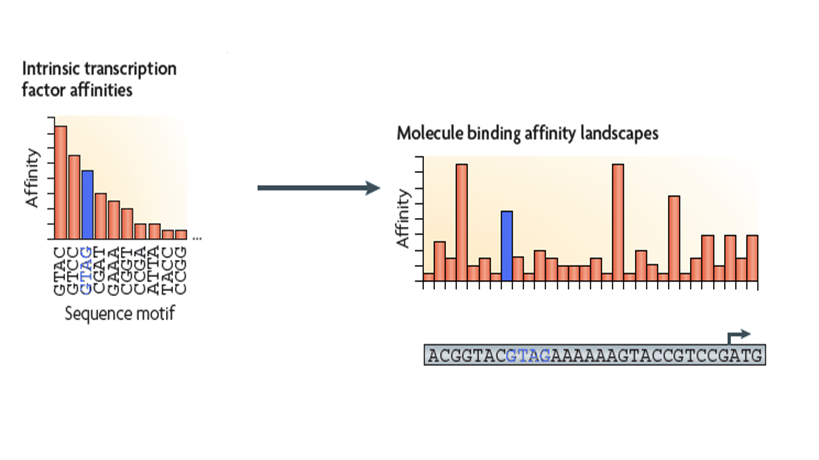
\includegraphics[width=1\textwidth]{segalblandscape}\\
  \caption{Widom, Segal Nature Review Genetics; "motif" denotes path through the PWM\cite{pmid19506578}}\label{sb}
\end{figure}
The partition function can be calculated by recursively moving through the matrix elements, in a way that is similar in spirit to standard algorithms of multiple sequence alignment\cite{BSA}, where we can think of each configuration as a possible way to 'align' each motif (PWM) to the CRM.  The variant of HMM's forward algorithm approach used by Segal for computing the partition function of all paths (configurations) is discussed in his supplementary material. 
\subsection{Enumerating the configurations of a CRM sequence }

 Here we will introduce a notation for the weights of many-binding site systems.  First, let $P(c)$, be the probability of a particular configuration (c) occurring
\begin{equation}\label{mbody}
    P(c) = \frac{W(c)}{\Sigma_c W(c)},
\end{equation}
where $ W(c)$ is the boltzmann factor or weight of the binding configuration, which is a list of occupations for each binding site locus within the CRM, where the occupation is either bound or unbound.   Using the notation of Xin, from Sinha lab ( which was using Buchler's model as a guide\cite{pmid20862354}\cite{pmid12702751}, a notation used by Terrell Hill that I followed in the Introduction of the Dissertation), we have:
\begin{equation}\label{wc}
    W(c)=  [\prod_i^N q(x)_{tf(i)} ] [\prod_{j}^{N-1} \omega_{tf(i),tf(j)}(d)]
\end{equation}
Here we have $N$ bound transcription factors, where $q(x)_{tf(i)}$ is the weight of the transcription factor for the ith binding site ($tf(i)$) that is $\textbf{bound}$ at position $x$ of the sequence, 
\begin{equation}\label{partitionf}
    q(x)_{tf(i)} = K_{s(x)}^{tf(i)} [tf(i)]
\end{equation}
Here $ K_{s(x)}^{tf{i}}$ is the equilibrium constant $K_a$ from equation \eqref{ka} for the binding site sequence $s$ binding by transcription factor $i$.  And $\omega_{i,j}$ is the interaction between the two $\textbf{bound}$ factors $tf(i),tf(j)$, where we have one less nearest neighbor interaction than the number of bound factors.  And $d$ is the distance separating factor $tf(i)$ from factor $tf(j)$ in units of base pairs ( $d = x(tf(i)) - x(tf(j))$ where $x(tf(i))$ is the sequence coordinate of factor $tf(i)$).
\subsection{The configuration vector nomenclature}

 Here we have used 'c' to denote the binding configuration of bound and unbound factors on the CRM following the symbol Segal used to denote the configuration, and we have used a map $tf(i)$ to link each binding site i to a transcription factor.  This map is similar to notation used by Segal, where he explicitly denotes the type of transcription factor at each bound site.
 
  Xin used a configuration vector, $\sigma$, which had indicator variables $\sigma_i$ for ith componenet of their configuration vector, where the ith component was the ith binding 'site'.  Xin's notation is elegant, in that every 'site' in their model is clearly represented in their configuration vector by the occupancy of the ith component of the vector.  
  
  Segal's notation does not display all the possible bound and unbound positions in the configuration (since there is a background occupancy in his model that causes unbound sequence to have a Boltzmann weight of 1.).  I have tried to stick to Segal's notation for a configuration by only displaying bound factors in the Boltzmann weight of a configuration, and by denoting explicitly the type of transcription factor at each bound site.  However, Segal's notation is based only on the CRM sequence, he does not actually have a 'site' notation, since every possible position in the CRM is considered a binding site for each transcription factor, and he simply looks at all the possible ways that coordinately regulating transcription factors could form monolayers on the CRM, without overlapping one another.  Hence, in Segal's notation, there really is no notion of a 'functional' site, as each \textit{possible} position within the CRM is a place for the factor to 'plant' itself (a place for the transcription factor to bind), where \textit{possible} is distinct from \textit{probable} by the use of PWMs.   
   
Seeing that binding sites are 'functional' (adaptations), or at least vestigals or exaptations, the notation of Xin for defining a 'site' we have tried to hybrid with Segal's notation.  Xin's notation is fundamentally based on binding 'sites' (adaptations).  For example, by either setting a threshold on a PWM to discover sites, or by knowing \textit{a priori} what are the binding 'sites' (regulatory adaptations), Xin starts the configuration problem (the notation) with N binding sites.  The indicator variables of the configuration vector are equivalent to occupancy of each site, hence $\sigma_i$ is either 0 or 1 for each component of the configuration vector.  For example:
\begin{eqnarray}
W(c)=W(\sigma)&=& W(\sigma_1,...,\sigma_{N} , \sigma_{1,1},..,\sigma_{N,N})\\
&=& \exp{(-\sum_i^N ln(q_i) \sigma_i - \sum_j^N ln(\omega_{ij}) \sigma_{ij})}
\end{eqnarray}
% \begin{equation}\label{}
%    W(c)=W(\sigma)= W(\sigma_1,...,\sigma_{N} , \sigma_{1,1},..,\sigma_{N,N}),
%\end{equation}
Here, $ln(q_i)$, is the free energy of binding to the $i$th site, and $\sigma_{i}$, denotes the occupancy of the $i$th 'site', and $\sigma_{ij}$ denotes the pairwise energetic interaction $ln(\omega_{ij})$ between site $i$ and site $j$\footnote{Recall for the canonical ensemble, where H is the Hamiltonian of a configuration we would have  $W(c) = \exp{-H(c)/kT}$ being a simple Boltzmann factor, where k$T$ is the thermal energy.  We are working in a grand canonical ensemble, which allows for particle energy as well as energy exchange, hence, the total energy of the configuration is a function of the Hamiltonian and the chemical potential of the factors, which causes concentration of the transcription factors to influence the total energy of a configuration, hence the energy is a thermodynamic free energy}.  But what type of transcription factor is binding to the $i$th site?  In Xin's notation, this is not decipherable.  Rather, in their notation, each 'site' corresponds to a particular factor.  But we simply don't know which factor.  Hence in Xin's notation it's possible that two distinct 'sites' occupy the exact same locus.  Hence we don't know if two sites are overlapping.  Overlapping sites can not both be bound, since all thermodynamic model's for occupancy of transcription factors use 'hard sphere potentials', there's steric hinderance prohibiting two transcription factors to occupy the same space along the CRM.).  Hence, in Xin's notation, one is supposed to be cognizant that bound overlapping sites will set that configuration's weight to zero. 

We have used a hybrid notation in Eq.\ref{wc}, where it's not that our CRM has N fixed binding sites (like in Xin's notation) that are each bound or unbound.  Rather, the weight $W(c)$ displays $N$ bound sites from a configuration c.  Hence, in our notation $N$ is a variable in the binding configuration space, while in Xin's notation, N is the fixed number of sites.  In Xin's notation, advantageously, they can put a bound on configuration space as $2^N$, this is an upper bound because overlapping sites will reduce the total number of configurations, furthermore this overcounts the number of unbound states, since a loci's sequence that match for multiple factors - say m factors- would consider $2^m/2-1$ too many configurations, since the loci is actually only unbound in one possible way\footnote{Xin's GEMSTAT computes the correct weights and partition function, it's just the estimate on the configuration space that is a bound.}.   
\subsection{An example of the hybrid configuration notation} 
For an example of the hybrid notation, consider all possible positions of the CRM as a binding site, as Segal would, and multiple morphogens binding to the same site ( same position within the sequence, same locus ); then the configuration vector (c) can be written in terms of Xin's indicator variables (similar to Ising models).  
 
For a length L CRM and for 3 transcription factor types (like Dorsal,Twist, and Snail) we have in Xin's notation $N =4*L$, where the factor of four is due to the four types of transcription factors at each locus - namely: bound by Dorsal, Twist, or Snail or 'background' (background is a type of pseudoparticle that fills the unbound state)).\footnote{As pointed out by Segal in his supplement, this problem may seem computationally infeasible, since the number of configurations for L=500 is of size $2^{4*500}$, but due to the forward algorithm it is possible.  Here the number of binding sites, $N$, neglects edge effects of k-mers requiring length k binding site sequences.  Hence, the calculation of the number of configurations is only a bound on the cardinaility of the set of configurations, where the bound is further affected by the neglect of overlapping sites that cause many configurations to be unaccessible (against the rules). } 

In this case, the vector of indicator variables is written as a matrix of size 4xL.  For example, for the toy CRM sequence 'acggt', we would have a configuration vector of size 20.  If we add another 'state' to the configuration vector denoted as 'silent' to represent steric effects, where the type of transcription factor indicator variable now only indicates the 'start' of a binding site, we would then have a indicator matrix of size 25, as indicated in Figure \ref{configurationMatrixI}, where the Dorsal transcription factor occupies positions 2 and 3 of the CRM (in this toy case Dorsal occupies a site just of length 2), and the rest of the CRM is occupied by the background factor.  Hence the configuration vector (a value of the matrix of indicator variables) is of size N+5 (the 5  due to the 'silent' states) assuming no interactions between bound factors.  If there are interactions, for example nearest neighbors, then there are an additional $\frac{16N^2}{2}$ components to the configuration vector, which we will not display.
 
\begin{figure}
  % Requires \usepackage{graphicx}
  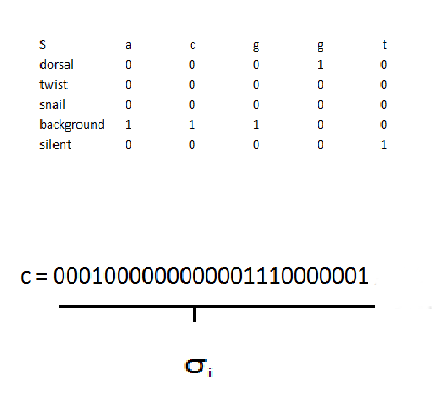
\includegraphics[width=1\textwidth]{configurationMatrixIb}\\
  \caption{The toy CRM sequence acggt is annotated at each of its loci ( positions ) to denote the configuration vector in row major ordering (1st five bits are dorsal's row, second five bits are twist's row etc...).  In the language of HMMs, the value of a configuration vector reveals the hidden state of the sequence.  Here there are 5 states, where the 'silent' state indicates a transcription factor is bound to an upstream position of the sequence, causing the loci to be covered by an internal position of the planted factor.  }\label{configurationMatrixI}
\end{figure}

Now that we have defined our configuration notation, and described the weight of a given configuration, we will explain in the next section our novel form of the pairwise interaction $\omega$ between bound factors.
%
%\begin{figure}
%  % Requires \usepackage{graphicx}
%  \includegraphics[width=1\textwidth]{1042015/HMM}\\
%  \caption{}\label{HMM}
%\end{figure}
%
%\begin{figure}
%  % Requires \usepackage{graphicx}
%  \includegraphics[width=1\textwidth]{"1042015/configuration"}\\
%  \caption{configuration or many-body state of the system}\label{configuration}
%\end{figure}

%%%%%%%%%%%%%%%%%%%%%%%%%%%%%%%%%%%%55ab

\subsection{The pairwise interaction $\omega$ between bound factors}
%
Transcription factors often interact with each other, causing certain configurations to be more likely by decreasing the total energy of the configurations where interacting factors are jointly bound, thereby increasing the weight of those configurations.  This observation, was the physical basis behind A. Hill's famous Hemoglobin Oxygen binding model.  

In the work of Xin a number forms of distance dependent pairwise interactions between bound factors was tested, such as sinusoidal functions over space that account for 'phasing' where one bound factor interacts with the nearest neighbor that is in phase (by using the major groove distance) with the factor of interest.  Similarly, gaussian decays from the center of the planted factor, and square functions were attemted and implemented.  Hence, GEMSTAT has a small database of pariwise interaction forms.  All the forms, as ours too, only allow for interactions between nearest neighbor bound proteins. 

For the the DV network interactions between Dorsal and Twist have been experimentally shown to be distance dependent, hence we use an interaction that is a function of the DNA basepair distance separating the nearest neighbors.  For the network that we are modeling this distance dependent interaction has been shown to be dominant force driving the Dorsal border of neuroectoderm expressed genes.  For the neuroectoderm network\footnote[2]{neuroectoderm network are the set of genes coordinately expressed in the lateral regions of the developing embryo, this developing tissue spans about 10 cells at the time point under consideration}  Crocker et.al. and Szymanski et.al. \cite{pmid7774581},\cite{pmid18986212}have shown that the spacing between sites plays a dominant role in defining the number of cells that are turned on in this region (width or span of cells).

For both the DV and AP (Anterior Posterior) network short range antagonistic interactions have been show to dominate the action of repressor transcription factors\cite{pmid20087339}.  The Snail transcription factor is a short range repressor acting to regulate the DV axis, which we also model using a distance dependent interaction, commonly called 'Quenching'\cite{pmid20087339}.
\begin{figure}
  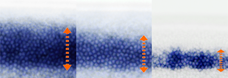
\includegraphics[width=1\textwidth]{rhoNEEs}\\
  \caption{ Changing the spacing between motifs in modules change the span of cells that are expressed.  In this Figure the spacing between two sites was adjusted by Natural Selection in orthologs of the \textit{rhomboid} gene's CRM. When the ortholog CRMs were transgenically inserted into \textit{mel} species the width of the expression pattern changes relative to the endogenous pattern width, suggesting that coopertivity between the sites is a function of the distance between sites that can be used by evolution to 'fine tune' the epression patterns in development.  When each sequence or module is expressed in its respective specie (lineage), then the relative widths (w/L where L is the lengths of the major axis of the specie's embryo, w is the width of the tissue in nanometers that express the gene) of the tissues are the same.  Different specie's embryos have different sizes hence there is a scaling law - how a characteristic (such as gene expression) changes with body size.  This Figure is from Erives Crocker et.al 2008 "Evolution acts on enhancer organization to fine-tune gradient threshold readouts. PLoS Biology"}\label{rhoNEEs}
\end{figure}

  Furthermore, since we do not know the exact form of the function, we bin the distance separating the proteins, and for each bin a free parameter is fit.  One may look for a coarse binning of the separation distance in bins of 10bp, or as fine as bins of 1bp.  If we choose the former option than an example of our protein-protein interaction parameter would be as follows:
\begin{equation}\label{}
   \overrightarrow{ \omega(d)} =  [ \omega_1 ,\omega_2 ,\ldots, \omega_b,\ldots,  \omega_n ]
\end{equation}
where the subscripts of the components of the $\omega$ vector (coopertivity or synergistic protein-protein interactions)  represent the corresponding bin ,b, ( in this case there are n bins), hence they define a bin vector, $\overrightarrow{B}$, where its components corresspond to the interval of base pair distances.

\begin{equation}\label{}
\begin{split}
 \overrightarrow{B}   &= [ B_1 ,B_2 ,\ldots, b, \ldots, B_n ] \\
     &=   [ (0-10), (11-20), \ldots,(41-50),\ldots, (x-L)]
    \end{split}
\end{equation}
Here bin b, is all interactions where two bound sites are separated by 41-50 basepairs, and x represents the last bin border, and L represents the Length of the module (sequence).  This representation of coopertivity vector, is really only useful for programming purposes, mathematically the coopertivity is simply a piecewise defined function:


\[
  \omega(d) =
  \begin{cases}
   \omega_1  & \text{ if } d \in (0,10)  \\
   \omega_2  & \text{ if } d \in (11,20)  \\
   \ \ \ \ \ \vdots \\
 \omega_n  & \text{if } d \geq x
  \end{cases}
\]

Our aim is to fit the biochemcial parameters that tune the probability of configurations that occur in live embryos.  However, we simply don't have such detailed biochemical experiments.  Hence, we use the mRNA of the target genes regulated by Dorsal Twist and Snail as a readout of what binding configurations are likely occurring, and wheter certain configurations have strong linkage (pairwise interactions) between certain bound factors.  Hence, we must infer from mRNA data, what is occuring at the DNA binding level; an expression to sequence model.  In the next section will describe a ubiquitous and obvious assumption, mRNA is caused by PolII, hence PolII binding is a proxy for gene expression.
 
\subsection{Relating the number of mRNA transcripts to fractional occupancy of PolII }
The amount of transcription that occurs at a gene locus is encoded in two segments of DNA sequence; first, the basal promoter that binds the Basal Transcription Apparatus (BTA), which is a massive complex of many proteins including PolII; second, and most important, the CRM that binds the morphogens or distal transcription factors (such as Dorsal) that modify and remodel the chromatin state and possibly have direct linkage with the BTA.  Hence the number of mRNA transcripts can be modeled as simply a linear relationship between the number of mRNA and the fractional occupancy of a promoter sequence (which we assume includes the CRM sequence).
\begin{equation}\label{}
     \left< N_{mRNA} \right>  \propto f_{BTA}.
\end{equation}
Of course, the occupancy of the BTA, $f_{BTA}$,  is a fraction this is at most one, hence $\left< N_{mRNA} \right> $ is the average number of mRNA molecules produced per nuclear cycle normalized by the maximum production rate over a cycle. 



 


%% Put the body of your dissertation here. 
%% DO NOT include the bibliography or any appendices.

%%%%%% LANDSCAPE PAGES  %%%%%%
%% To produce text, graphics or tables in landscape mode, 
%% use the following template. Begin be removing the single "%" signs below.
%\begin{landscape}
%\thispagestyle{empty}
%\begin{minipage}{\linewidth}
%% Insert the graphics or table that is to be in landscape mode.
%% Use the figure or table environment. You may wish to center the float. 
%\end{minipage}
%\end{landscape}

%%%%%%%    APPENDICES    %%%%%%%%%%
%% If you wish to include one appendix, remove the "%" from the 
%% following two lines.
%\renewcommand{\appname}{APPENDIX}
%\appendix
%% To include several appendices, remove the only the "%"
%% in front of "\appendix".

%% In either cast to start your first appendix, which will be labeled
%% as Appendix A, just type \chapter{<appendix 1 name>}
%% and enter the text of the appendix as you would a chapter.

%%%%%%% A NOTE ABOUT APPENDICES %%%%%%%%%
%% Some appendices may be single spaced such as survey examples
%% or letters. Contact the Graduate School for details.
%% To single space an appendix first remove the "%" from 
%% the following two lines.
%\end{doublespace}
%\chapter{<appendix name>}
%% Insert the name of the appendix.
%% Insert the text of the appendix.
%% Remove the "%" from the following line.
%\begin{doublespace}
%% Any text entered now will be double spaced.

\end{doublespace}

%%%%%%  Bibliography %%%%%
%% A bibliography is required. By default it is called, "Bibliography"
%% You may use �Literature Cited�, �Works Cited� or �References� 
%% instead of �Bibliography� if that is the convention in your discipline. 
%% To do so, place your choice in the  empty argument 
%% of the following command and remove the "%".
%\renewcommand{\bibname}{}

%% The bibliography may be made using BibTeX.
%% To do so the necessary commands must be entered in the 
%% preamble and here.
%% If the Bibliography is made from scratch,
%% remove the "%" in front of "\begin{thebibliography}{???}"
%% replacing the ??? with the appropriate entry and 
%% remove the "%" in front of "\end{thebibliography}"
% \begin{thebibliography}{???}
%%  Enter the bibliography here.
% \end{thebibliography}
%% In either case, the bibliography is automatically entered
%% in the Table of Contents.


\bibliographystyle{plain}

\bibliography{sample}

\end{document}

%%%%%% A FINAL COMMENT %%%%
%% Once your document has been filed with the Graduate School,
%% if you wish to produce a single spaced version of your document, 
%% find and remove the two commands \begin{doublespace}
%% and \end{doublespace} above.
